\documentclass{report}

\usepackage{appendix}%for additional appendix options
\usepackage{float} %when using [H]: figure placed at exact spot
\usepackage{graphicx}
\usepackage{verbatim} % for multi-line comments
\usepackage{listings}
\usepackage{amsmath}
\usepackage[pict2e]{struktex}
\usepackage{parcolumns}
\usepackage{multirow}
\usepackage{pstricks}
\usepackage{enumerate}% to be able to customize enumeration lists 
\usepackage[tight]{subfigure}%tight für weniger platz zwischen figures, see subfigrue docu
% \usepackage{multicol}
%\usepackage[rflt]{floatflt}

%\usepackage{fullpage}

%I've found the following lines in the internet to automatically begin a new line after a paragraph
\newcommand{\norm}[1]{\left|#1\right|}
\newcommand{\nnorm}[1]{\left|\left|#1\right|\right|}

\makeatletter
\renewcommand\paragraph{\@startsection{paragraph}{4}{\z@}%
  {-3.25ex\@plus -1ex \@minus -.2ex}%
  {1.5ex \@plus .2ex}%
  {\normalfont\normalsize\bfseries}}
\makeatother

%modification of page-margins
\addtolength{\hoffset}{-1.3cm}
\addtolength{\textwidth}{3.5cm}
%\addtolength{\textheight}{0cm}

%to change section numbering depth to 3 (default 2)
\setcounter{secnumdepth}{3}

%to change depth for appearence in table of contents to 3 (default 2)
\setcounter{tocdepth}{3}

\begin{document}

%% \documentclass[12pt]{article}

% \usepackage{ngerman}
% \selectlanguage{ngerman}
% \usepackage[latin1]{inputenc}

% \usepackage{graphicx}

% \begin{document}

\pagestyle{empty}

\begin{center}

\vspace*{-2.8cm}
\begin{minipage}[c]{.30\textwidth}
  \begin{flushleft}
    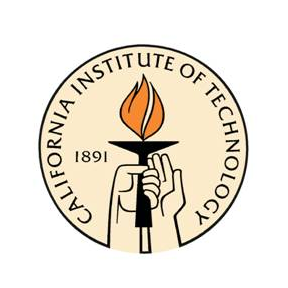
\includegraphics[width=3cm,clip=]{LOGO/caltech_logo}%
  \end{flushleft}
\end{minipage}
\begin{minipage}[c]{.43\textwidth}
\vspace*{1em}
    {GALCIT (Caltech)\\Prof. Hans G. Hornung \\ \\ Institute of Aerodynamics (TUM) \\ Prof.~Dr.-Ing. N.~A.~Adams}%
\end{minipage}
\begin{minipage}[c]{.25\textwidth}
  \begin{flushright}
    \vspace*{1em}
    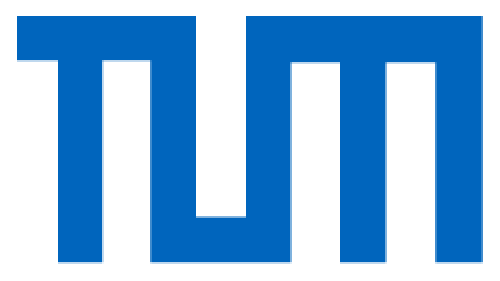
\includegraphics[width=3cm,clip=]{LOGO/TUMLogo_oZ_Vollfl_blau_RGB}%
  \end{flushright}
\end{minipage}

\vspace*{3.3cm}
\begin{minipage}[c]{11cm}
{\LARGE\bf 
Simuation of high enthalpy flow in porosities using SPH}
\end{minipage}

\vspace*{0.8cm}
Oliver Oberinger\\

\vspace*{2.8cm}
{\bfseries Diplomarbeit}

\vspace*{1.2cm}
%\large
\normalsize
\vfill
\begin{tabular}{ll}
Betreuer: & ~Prof. Hans G. Hornung (Caltech)\\
\ & \ Dipl.-Ing. Sergey Litvinov (TUM)\\
 \\
Ausgabe: & 15.\ Juni 2010\\
Abgabe: & 15.\ Dezember 2010\\
\end{tabular}

\vspace*{1.6cm}
%\large
Institute of Aerodynamics Technische Universit\"{a}t M\"{u}nchen\\
Graduate Aerospace Laboratories California Institute of Technology\\
2010	
\end{center}

\pagebreak
\pagestyle{plain}

%\end{document}


%% \documentclass[12pt]{article}

% \usepackage{ngerman}
% \selectlanguage{ngerman}
% \usepackage[latin1]{inputenc}

% \usepackage{graphicx}

% \begin{document}

\pagestyle{empty}

\begin{center}

\vspace*{-2.8cm}
\begin{minipage}[c]{.30\textwidth}
  \begin{flushleft}
    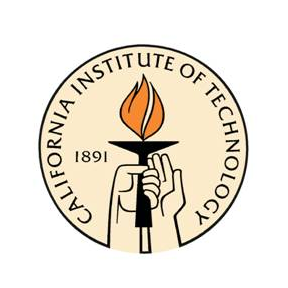
\includegraphics[width=3cm,clip=]{LOGO/caltech_logo}%
  \end{flushleft}
\end{minipage}
\begin{minipage}[c]{.43\textwidth}
\vspace*{1em}
    {GALCIT (Caltech)\\Prof. Hans G. Hornung \\ \\ Institute of Aerodynamics (TUM) \\ Prof.~Dr.-Ing. N.~A.~Adams}%
\end{minipage}
\begin{minipage}[c]{.25\textwidth}
  \begin{flushright}
    \vspace*{1em}
    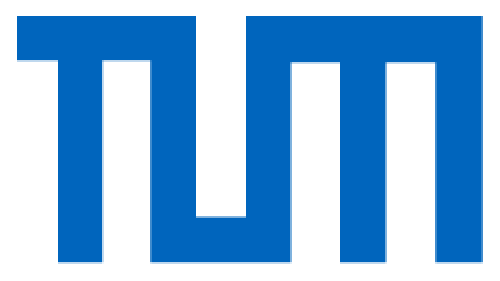
\includegraphics[width=3cm,clip=]{LOGO/TUMLogo_oZ_Vollfl_blau_RGB}%
  \end{flushright}
\end{minipage}

\vspace*{3.3cm}
\begin{minipage}[c]{11cm}
{\LARGE\bf 
Simulation of high enthalpy flow in porosities using SPH}
\end{minipage}




\vspace*{1.0cm}

Oliver Oberinger\\
\vspace*{1.0cm}
{\bfseries Intermediate version of Master's Thesis}\\
\vspace*{0.5cm}
for presentation at \\
\vspace*{0.3cm}
Institut Sup\'{e}rieur de l'A\'{e}ronautique et de l'Espace\\


\begin{minipage}[c]{.25\textwidth}
	
\includegraphics[width=3cm,clip=]{LOGO/LogoISAE}\\
\end{minipage}
\\
\vspace*{0.1cm}
responsible at ISAE: J\'{e}r\'{e}mie Gressier (Professeur SUPAERO)





\vspace*{1.2cm}
%\large
\normalsize
\vfill
\begin{tabular}{ll}
Advisors: & ~Prof. Hans G. Hornung (Caltech)\\
\ & \ Dipl.-Ing. Sergey Litvinov (TUM)\\
\ & \ Prof. Dr.-Ing. Nikolaus A. Adams (TUM)\\
 \\
\end{tabular}

\vspace*{1.6cm}
%\large
Institute of Aerodynamics Technische Universit\"{a}t M\"{u}nchen\\
Graduate Aerospace Laboratories California Institute of Technology\\
2010	
\end{center}

\pagebreak
\pagestyle{plain}

%\end{document}


% \documentclass[12pt]{article}

% \usepackage{ngerman}
% \selectlanguage{ngerman}
% \usepackage[latin1]{inputenc}

% \usepackage{graphicx}

% \begin{document}

\pagestyle{empty}

\begin{center}

\vspace*{-2.8cm}
\begin{minipage}[c]{.30\textwidth}
  \begin{flushleft}
    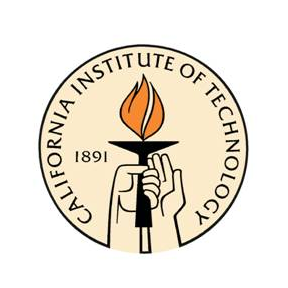
\includegraphics[width=3cm,clip=]{LOGO/caltech_logo}%
  \end{flushleft}
\end{minipage}
\begin{minipage}[c]{.43\textwidth}
\vspace*{1em}
    {GALCIT (Caltech)\\Prof. Hans G. Hornung \\ \\ Institute of Aerodynamics (TUM) \\ Prof.~Dr.-Ing. N.~A.~Adams}%
\end{minipage}
\begin{minipage}[c]{.25\textwidth}
  \begin{flushright}
    \vspace*{1em}
    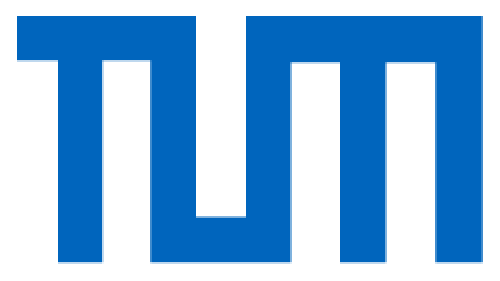
\includegraphics[width=3cm,clip=]{LOGO/TUMLogo_oZ_Vollfl_blau_RGB}%
  \end{flushright}
\end{minipage}

\vspace*{4.3cm}
\begin{minipage}[c]{11cm}
{\LARGE\bf 
Simulation of high enthalpy flow in porosities using SPH}
\end{minipage}




\vspace*{1.0cm}

Oliver Oberinger\\
\vspace*{1.0cm}
{\bfseries Master's Thesis}\\
\vspace*{0.5cm}

\vspace*{3cm}




\vspace*{1.2cm}
%\large
\normalsize
\vfill
\begin{tabular}{ll}
Advisors: & ~Prof. Hans G. Hornung (Caltech)\\
\ & \ Dipl.-Ing. Sergey Litvinov (TUM)\\
\ & \ Prof. Dr.-Ing. Nikolaus A. Adams (TUM)\\
 \\
\end{tabular}

\vspace*{1.6cm}
%\large
Institute of Aerodynamics Technische Universit\"{a}t M\"{u}nchen\\
Graduate Aerospace Laboratories California Institute of Technology\\
2010	
\end{center}

\pagebreak
\pagestyle{plain}

%\end{document}




\tableofcontents
\chapter{Introduction}
\label{sec:intro}


This work aims at the numerical simulation of high enthalpy flow over a porous
surface. The subject is of interest, as experiments CITATION
NEEDED (Prof. Hornung) have shown that wall porosity can damp
acoustic instabilities in hypersonic flows over a slender cone. In the long term, a numerical simulation of this configuration is desired to furnish data for a detailed analysis of the active mechanism. A first approach to this objective is done by the present work which tempts to simulate a simplified porosity configuration with a simulation method called Smoothed Particle Hydrodynamics (SPH). 

SPH designates a mesh-free method for numerical simulation of particle
ensembles, respectively matter that can be modeled as an ensemble of
particles as is the case for fluids.
Thus, the term particle ensemble not only refers
to fluids (as the name of the method would suggest) but also to solids. In
fact, nowadays, SPH is employed to simulate problems in different fields,
such as elasticity and fracture of solids, liquid flows and gas
dynamics~\cite{Monaghan2005}.
The initial development of the method dates back to 1977, when Gingold and
Monaghan \cite{Gingold1977} tempted to compute an astrophysical %(gas dynamics - I am not sure if it's actualy a gas dynamics problem) 
problem with a new, compared to grid based methods more efficient approach. Independently and simultaneously, work in this field was also carried out by Lucy who came up with the same idea~\cite{Lucy1977}. One main advantage of SPH, which also is the reason why SPH was applied first to astrophysical problems, lies in the fact that it is a particle method and therefore does not need any room-fixed grid for the underlying numerical scheme. Instead, the base for the calculation of derivatives are discrete points, the particles, which move with the fluid (Lagrangian approach). Dealing with high density variations and huge calculation domains, astrophysical problems, when simulated with grid-based methods, 
required a considerable effort in terms of mesh--refinement. For particle methods like SPH however, density variations are principally resolved naturally by a more or less dense particle spacing and calculation is only performed at places where there is matter, i.\ e.\ particles.
Another advantage of the method not requiring a meshing, is the relative ease of the implementation of complex boundary geometries. And this is the main reason for the application of SPH in this work, as the structure of the solid boundaries represents a significant part of the problem, when treating porosities. 
 
%OTHER APPROACHES FOR CAVITY/POROSITY SIMULATION (look up in literature)
To be able to perform the simulation, a 2D compressible SPH code was developed in several stages and then validated by means of various test cases.

The first code that emerged from this project was a simple 1D compressible SPH code simulating a shock--tube problem. Although this code has no real use for practical applications, it is presented in this thesis with the goal to introduce the reader, who would like to familiarize himself with the implementation of SPH, to this technique.

The subsequently developed 2D code is based on an incompressible multi--phase SPH code, which was developed by \cite{Hu2006} and is now in use at the Institute of Aerodynamics of the TUM. This code was adapted in several steps to the needs of the present work, the first step being the implementation of the equations used in the 1D SPH code mentioned above and thus, the adaption of the code to treat inviscid compressible problems. At this stage the code was tested for accuracy and robustness by means of the 1D shock--tube problem. Both a 1D and a 2D particle distribution have been employed to this 1D problem. To conclude the 1D shock--tube tests, a study on the influence of perturbations in the initial particle distribution has been conducted, again both for 1D and 2D particle fields.
At the same point, the simulation of acoustic wave propagation has been assessed, as acoustic phenomena are essential for the final flow configuration to investigate (see above).
In a next step the code was further adapted to incorporate physical viscosity and heat conduction models. The correctness of the implemented viscosity model was tested by analyzing the temporal decay of vortices using the Taylor--Green flow and the thermal conduction model was validated with a standard problem of pure heat conduction.
The final test--case, which is a compressible Couette flow with hot and cold wall boundary conditions, combined all of the previously implemented models. It demonstrated that the combination of all the models would work with the required accuracy.
Finally, after the systematic validation of all components of the flow model, the flow through porosities and over a porous surface is simulated exemplary by means of two different porous configurations. 

The structure of this document is based on the classical structure of a scientific paper \cite{Day2006}, with the four chapters Introduction, Methods, Results and Discussion/Conclusion. If, when looking at the table of contents, the detailed organization of this document does not appear logical to the reader, the following lines are intended to point out the idea behind it.
In a first section (\ref{sec:sec:BasicsSPH}), the Methods-chapter briefly describes the theoretical idea behind the SPH-method. The second section (\ref{sec:ElementsOfSPH}) deals with some essential components of an SPH-implementation, followed by a section (\ref{sec:GenIntroTestCases}) generally introducing the test-case problems and giving their analytical solutions, where available. The general presentation of the test cases figures at this spot, as it is needed in the following sections. The next two sections (\ref{sec:1DSPHcode}) and (\ref{sec:1DSPHcode}) explain the developed SPH-codes and also describe how to run them. Subsequently, there is a section (\ref{sec:simuSetupTestCases}) describing the detailed simulation setup and post-processing procedure for each test-case, so that every result presented in this document may be exactly reproduced with the information given in this section.
In the following chapter (\ref{sec:Results}), the results of all test cases as well as the porosity simulations are presented and the final chapter (\ref{sec:conclusion}) concludes the work and gives a brief future perspective.

\chapter{Method}
\label{sec:method}
\section{Basic Idea of SPH}
\label{sec:BasicsSPH}

To illustrate the basic idea of SPH, it is helpful to first consider the
governing equations of fluid dynamics for an inviscid flow, the Euler equations.  As SPH has its origin in Astrophysics, and as many astrophysical problems can be modeled by the Euler equations \cite{Liu2003}, it is these equations, on which the SPH formalism is based on its original form. 

%\begin {equation}
%Euler IN LAGRANGIAN FORM
%\end {equation}

%The above equations have the form~\cite{Monaghan2005}
The Euler equations have the form~\cite{Monaghan2005}

\begin {equation}
\label{eq:EFD_form}
{\frac{dA({\bf r})}{dt}}=f(A({\bf r}),\nabla A({\bf r}),{\bf r})
\end {equation}
where
\begin {equation}
{\frac{d(.)}{dt}}={\frac{\partial(.)}{ \partial t}}+u\nabla(.)
\end{equation}
is the substantial derivative.

Thus the rate of change of a physical quantity depends on its spatial
derivatives. The goal of any method for numerical simulation is to approximate
these derivatives by information of a discrete number of points only in order for a computer to be able to handle it. 

\subsection{Integral approximation}

The SPH method is based on the idea of approximating a function $A(x)$ by an
integral interpolant
\begin{equation}
\label{eq:int_interpolant}
A_I({\bf r})=\int A({\bf r'})W({\bf r}-{\bf r'},h)d{\bf r'}
\end{equation}
%\begin{equation}
%A({\bf r})=\int A({\bf r'})\delta({\bf r}-{\bf r'})d{\bf r'},
%\end{equation}
where $W({\bf r}-{\bf r'},h)$ is the so called {\tt kernel function} or {\tt smoothing function} and $h$ the
{\tt smoothing length}. If $W$ is the delta function this expression is exact,
otherwise it represents an approximation. As the theoretically
perfect kernel, the delta function, is of no practical use, the kernels
employed in practice are functions which tend to the delta function in the 
limit $h\rightarrow 0$.
Examples for those kernel functions are a Gaussian kernel or
kernels based on Schoenbergs~\cite{Schoenberg1946} $M_n$ splines~\cite{Monaghan2005}.
More details on SPH kernels are given in section
(\ref{sec:KernelFunction}) and in the book on SPH published by Liu~\cite{Liu2003}.

The fact of using a kernel different from the delta function constitutes the
first of two approximations made by the SPH method. It is often referred to as {\bf kernel approximation}~\cite{Liu2003} or integral approximation.

\subsection{Particle approximation}
The second approximation consists of a discretization of the integral
expression in equation~(\ref{eq:int_interpolant}), thus changing the integration
to a summation over all discretized elements of the domain - the particles. 
This allows for the determination of $A_I(\bf{r})$ by numerical methods. In the SPH
literature, this second approximation is commonly called {\bf particle
approximation}~\cite{Liu2003}.

With the relation between mass, density and volume for each discretized particle
\begin{equation}
m_i=\rho_i V_i,
\end{equation}
applying the particle approximation to equation (\ref{eq:int_interpolant}) leads to the following expression:

\begin{equation}
\label{eq:intInter}
A_S({\bf r})=\sum_b m_b \frac{A_b}{\rho_b}W({\bf r}-{\bf r}_b,h).
\end{equation}
This equation states that an estimate of a function at a certain position ${\bf r}$ can be obtained by interpolation using the discrete points, the particles $b$, of the calculation domain. 


\subsection{Approximation of derivatives}

As mentioned at the beginning of this section (\ref{sec:BasicsSPH}), the objective is to find an approximative expression for change rates or derivatives.
With the ideas introduced so far, this can easily be obtained by just deriving the above equation (\ref{eq:intInter}), which gives~\cite{Monaghan2005, Liu2003} 
%(in Liu with gradient,im Monaghan for 1 direction)

\begin{equation}
\label{eq:simpleDerivative}
\nabla A_S({\bf r})=\sum_b m_b \frac{A_b}{\rho_b}\nabla W({\bf r}-{\bf r_b},h).
\end{equation}
and shows that in SPH the derivative is approximated by an exact derivation of an approximative function, the kernel function.

The disadvantage of the above equation (\ref{eq:simpleDerivative}) however is, that for
$A(\bf{r})=const.$ the approximated derivative does not vanish. By using the identity
%(in Monaghan the equation figures not with gradient but only in 1 direction!?!)
\begin{equation}
\label{eq:derivativeIdentity}
\nabla A = \frac{1}{\Phi}(\nabla {\Phi A}-A\nabla \Phi),
\end{equation}
where $\Phi$ is any differentiable function, this problem can be resolved \cite{Monaghan2005}. In its
SPH form equation (\ref{eq:derivativeIdentity}) reads as follows:

\begin{equation}
\label{eq:genFirstDerivativeSPH_Approximation}
\nabla_a A = \frac{1}{\Phi_a}\sum_b \frac{m_b \Phi_b}{\rho_b}(A_b-A_a)\nabla_a W_{ab}.
\end{equation}
This is the general approximation form for a first derivative in SPH. Depending on the choice for $\Phi$ different approximative expressions result. Widely used in literature are $\Phi=1$ and $\Phi=\rho$ leading to the following derivative approximations:
\begin{equation}
\label{eq:genFirstDerivativeSPH_Approximation_Phi_1}
\nabla_a A = \sum_b \frac{m_b}{\rho_b}(A_b-A_a)\nabla_a W_{ab}.
\end{equation}
\begin{equation}
\label{eq:genFirstDerivativeSPH_Approximation_Phi_rho}
\nabla_a A = \frac{1}{\rho_a}\sum_b m_b (A_b-A_a)\nabla_a W_{ab}.
\end{equation}

\subsection{Application of SPH principles to Euler equations}

Now that the basic SPH idea is introduced, both the field function
itself and its spatial derivatives can be approximated using only known information of a discrete number of particles. Hence, the rates of change of
the quantities $\rho,v, e$ described by the Euler equations of fluid dynamics, which are of the form
corresponding to equation (\ref{eq:EFD_form}), can be rewritten using this information. Thus 
one obtains the SPH formulation of the equations of fluid dynamics.

The detailed derivation of the SPH equations for fluid dynamics will not be shown here, as the interest  only lies in describing the principle ideas behind the SPH
method. Depending on the transformations used, the final SPH equations can assume a different form. In the following, a common form for the rates of change of density, velocity and
internal energy based on the Euler equations, i.\ e.\ without viscosity and heat conduction, is listed \cite{Monaghan2005,Liu2003}: 
%(perhaps also list NSG-form, and
%explain why Euler is of interest as well (for 1DSPH code, perhaps later real
%code including viscosity???)

\begin{equation}
\label{eq:DCR_Euler}
\frac{d\rho _a}{\mathit{dt}}=\sum_b{m_{b}{\bf u_{\mathit{ab}}}\nabla _{a}W_{\mathit{ab}}},
\end{equation}

\begin{equation}
\label{eq:VCR_Euler}
\frac{ d {\bf u_{a}}}{\mathit{dt}}=-\sum_b {m_{b}\left(\frac{P_{a}}{\rho_{a}^{2}}+\frac{P_{b}}{\rho _{b}^{2}}\right)\nabla_{a}W_{ab}},
\end{equation}


\begin{equation}
\label{eq:ECR_Euler}
\frac{de_{a}}{\mathit{dt}}=-\mathit{}\frac{1}{2}\sum_b{m_{b}\left(\frac{P_{a}}{\rho _{a}^{2}}+\frac{P_{b}}{\rho _{b}^{2}}\right){\bf u_{\mathit{ab}}}\cdot\nabla _{a}W_{\mathit{ab}}}.
\end{equation}

As far as the SPH form of the continuity equation (equation (\ref{DCR_Euler}) is concerned, one can note, that it results directly from the application of (equation \ref{eq:genFirstDerivativeSPH_Approximation_Phi_rho}) to the continuity equation.

For the detailed derivation and for alternative formulations of
these equations refer for example to \cite{Monaghan2005, Liu2003}.

\subsection{Summary of SPH idea}
A field-function can be
described as an integral interpolation over the function itself and a kernel
function, which has to be chosen in an appropriate way (c.\ f.\ section (\ref{sec:KernelFunction})). This step introduces the smoothing length $h$ as a first approximation parameter. A further
approximation consists in transforming the integral over the domain into a
summation over the discrete elements - the particles - constituting this domain. This step introduced the particles as discrete elements with the particle spacing $dx$ being the second approximation parameter. 
These approximations allow to express both the field function and its spatial derivatives in a form that depends exclusively on discrete values
of the field function itself (and of the kernel function and its derivatives, 
all of which are known). By finally choosing an appropriate kernel function $W$ with compact support, i.\ e.\ a finite support domain, where $W=0$ beyond, the summation over all particles in the calculation domain can be reduced
to a summation over those particles within the support domain of the particle
in question.
The SPH formulation of the equations of fluid
dynamics is obtained by applying the above principles and conducting different
transformations to the original differential equations. 


%\section{Implementation of an SPH code}
\section{Elements of an SPH code}
\label{sec:ElementsOfSPH}
This section presents the elements of an SPH code. For some elements, there are different approaches or models, which are then briefly described and introduced. Emphasis however is placed on these variants that will finally be implemented in one of the two SPH codes designed and modified during this work.

Points of interest are a closer description of the kernel function, different methods to perform the search for the interacting particles, as well as the implementation of different boundary conditions in SPH. Furthermore, an
equation of state is introduced followed by a passage
explaining the need of artificial viscosity. The challenges of implementing a physical viscosity model and a heat conduction model are highlighted thereafter. Subsequently, some numerical integration schemes that have proved to be reliable for SPH applications are discussed and the two different possibilities to calculate the density are shown. Finally a general structure of a generic SPH code is given.

Note: in this section the above mentioned features are discussed in a general perspective, independently of the implementation in a particular code. The latter will be done in section (\ref{sec:CompAndStruc1DCode}) for the 1D code and in sections (\ref{sec:Comp2DCode}) and (\ref{sec:Struc2DCode}) for the 2D code which gives a more complete view.




\subsection{Kernel function}
\label{sec:KernelFunction}
% ???not sure, if its the right place here, but somewhere there should be a
% paragraph with more detailed information on kernels used, compact support,
% perhaps even some properties,...(and perhaps some graphics???)


Some properties of kernel functions, also called smoothing functions, and notions related to them have already been mentioned in section
(\ref{sec:BasicsSPH}). 

In principle, every function can act as kernel function
if it respects a set of criteria listed by~\cite{Liu2003}.
The most important ones are:
\begin{itemize}
\item The smoothing function should vanish outside of a certain area around its
center. This property, which is expressed in equation (\ref{eq:compactSupport}), is called compact support and the domain where $W\neq0$
is the {\bf support domain} of the smoothing function.  The support domain is characterized by its radius, the so called {\bf support length} $l_s$. In SPH literature however, the so called {\bf smoothing length} $h$ is more common, especially for the definition of the kernel functions. The relation between these two quantities is $l_s=\kappa h$ where $\kappa$ is a constant value and in general $>1$. Support length $l_s$ and smoothing length $h$ are not to be confused.
 
\begin{equation}
\label{eq:compactSupport}
W(x-x')=0,\textit{ \ for \ }|x-x'|>\kappa h
\end{equation}

\item The smoothing function should be normalized to 1, which ensures that constants
are interpolated exactly:
\begin{equation}
\int{W(x-x',h)dx'}=1.
\end{equation}

\item The smoothing function should tend towards the delta function as the smoothing
length $h$ tends to zero:
\begin{equation}
\lim\limits_{h \rightarrow 0}{W(x-x',h)}=\delta(x-x').
\end{equation}
This is to ensure consistency of the integral approximation, which means that
the approximate expression tends to the exact expression of the integral
interpolant equation for $h \rightarrow 0$.
\end{itemize}
The above list does not contain all necessary SPH kernel properties. Its complete version can be found in \cite{Liu2003}.
Based on these properties a variety of kernels are used in SPH literature. A
very commonly used kernel is the $M_4$ kernel (cubic spline) based on Schoenberg's
$M_n$-Splines~\cite{Schoenberg1946}, which reads with $q=\frac{\norm{x}}{h}$:

\begin{equation}
\label{eq:cubicSpline}
M_{4}(x)=\begin{cases}
\frac{1}{6}[(2-q)^{3}-4(1-q)^{3}],& \text{for 0 $\leq$ q $\leq$ 1} \\
\frac{1}{6}(2-q)^{3},&  \text{for 1 $\leq$ q $\leq$ 2} \\
O,& \text{for q $>$ 2}.
\end{cases}
\end{equation}
In this formulation the cubic spline kernel has a support of $l_s=2h$.				
Note: the above considerations were conducted in 1D, they apply equivalently to 2D and 3D.

In the work of \cite{Fulk1996} a measure of merit for kernels was developed and
they came to the result that, at least in 1D, no kernel performs significantly better than the cubic spline.
This is why for the 1D SPH code described in section (\ref{sec:1DSPHcode}) the cubic spline kernel was employed.

The unit of the kernel function $W$ is the inverse of the volume or the corresponding 1D/2D equivalent, as can be seen easily from equation (\ref{eq:SumDensity}) which is only introduced below.


\subsection{Neighboring particle search methods}
\label{sec:NNPS}
To calculate the derivatives in equations (\ref{eq:DCR_Euler})-(\ref{eq:ECR_Euler}), principally a
summation over all particles has to be performed. However, as the kernel
functions $W$ were defined with a compact support, i.\ e.\ $W=0$ beyond a certain distance from the particle in question, only particles within this distance, the so called support length (see section (\ref{sec:KernelFunction})), contribute to the interpolation of the origin particle's values, and thus interact with it. Finding the interacting particles is one of the key features in an SPH implementation, as an effective interaction search method, often also called {\bf nearest neighboring particle (NNP) search} method in the SPH literature, can considerably reduce computation time. 

The most basic NNP algorithm is called {\bf all pair search}, and as its name
suggests all imaginable particle pairs are tested for interaction. This means
that the calculation process consists of a double loop where the outer loop
iterates over all particles of the calculation domain and defines one of the pair's partners (often
referred to as origin). For each of the (origin) particles an inner loop is
performed, which iterates again over all particles thus defining the other
partner (destination) of the pair. Then, the pair is tested for the
interaction condition, meaning that their distance has to be smaller than the
support length. In this way, for a calculation domain consisting of $N$
particles, $N\cdot N$ iteration steps and tests have to be executed. The
calculation cost of this approach is therefore of the order of $O(N^2)$. 
If the interactions are assumed to occur pairwise, i.\ e.\ if there is a spatially constant
smoothing--, and therefore support--length,
%THINK ABOUT THE AVERAGED SMOOTHING LENGTH...)
there is a simple but efficient way of reducing computation
time: if a pair $P_{ab}$ is an interaction, the pair
$P_{ba}$ is an interaction as well. That way half of the $O(N^2)$ iterations
and tests can be eliminated, leading to a complexity of $O(N!)$. 
%(LOOK FORREFERENCES). 
This approach is employed in the 1D SPH code as it is easy to
implement \cite{Liu2003} and the number of particles in this 1D simulation is
still reasonably low in order not to have to use more sophisticated algorithms
such as these introduced right below.

A more effective but also more complicated method is the {\bf linked list
algorithm}. It is based on the fact that kernels with compact support are
used and thus interacting particles may only be located in the neighborhood of
the particle under consideration. The computation domain is divided into cells with
cell size $\ge \kappa h$, ideally $=\kappa h$, and the
particles are assigned to the cell they are located in~\cite{Monaghan1983}. In this way the cell
structure serves as a book--keeping device and in case of an interaction
calculation with an origin particle $a$ not all the particles $b,b={1,...,N}$ have to be considered but only those particles in the adjoining cells. Hence, the
complexity of the original problem which is of order $O(N^2)$ can be reduced
considerably and even tends to $O(N)$ if the particles in one cell are few compared to the total number of particles in the calculation domain. 
%FIGURE: DIAGRAM WITH CELLS /PARTICLES /DOMAIN!?!
Technically the cells are managed by the implementation of a linked list
structure in a computational code. More details on this are given in \cite{Monaghan1985, Hockney1988} and besides in section
(\ref{sec:2DSPHcode}), as this algorithm is implemented in the 2D
SPH code.
However, the method has a drawback if used with a spatially variable smoothing
length. In this case the cell size is not ideally adapted to every particle
and the algorithm looses efficiency.

Moreover, different other NPP techniques exist which shall not be introduced in
detail here. One class of these are called {\bf tree search algorithms}~\cite{Hernquist1989}, which are
especially robust and efficient for problems with variable smoothing
length~\cite{Liu2003}.
% and therefore are implemented in many astrophysical applications, as h=variable essential due to the huge variation of quantities


\subsection{Boundary condition implementation}
\label{sec:boundaryConditionImplementation}
For particles at the edge of the calculation domain, the summation interpolation does not
give exact results, as the integral (or better the sum) is truncated due to
the simple fact that outside the domain there are no
particles~\cite{Liu2003}. This effect is called the particle deficiency problem \cite{Liu2003}. %In cases where the region of interest is far from boundaries and where information from the domain edges does not propagate to the region of interest in the time of interest, there is no need to consider this problem. The 1D shock tube simulation with 1D particle distribution described further below (PERHAPS LINK TO SECTION)is an example of such a case. But for many applications precise boundary conditions have to be applied and it is therefore necessary to treat the edges of the domain in a special manner, depending on the desired boundary condition. This often includes the placement of so--called virtual particles or ghost particles within the distance of one support length outside the domain, which are assigned properties according to the boundary condition to implement.
It can also be interpreted in a physically correct way %(stimmt das genau, oder gibt es totzdem einen Fehler, auch bzgl. vacuum? Monaghan05 p.37: near boundaries error of a few percent...) 
as a free surface, i.\ e.\ a bordering of the calculation domain to the vacuum. Free surfaces are therefore modeled naturally by SPH being a particle method. If the domain however is not bordered by free surfaces but a wall or other types of boundary conditions such as symmetrical or periodical, the edges have to be treated in a special way. This often includes the placement of so--called virtual particles or ghost particles within the distance of one support length outside the domain, which are assigned properties according to the boundary condition to implement. These virtual particles, that were originally used by \cite{Libersky1993} for SPH, then contribute to the calculation of the quantities of the real particles inside the domain. Thus the particle deficiency problem can be solved and the boundary is not considered by the simulation as a free surface but as the desired boundary type. 

The following paragraphs detail this and alternative concepts for the different types of boundary conditions

\subsubsection{Periodical boundary condition}
The periodical boundary condition is relatively easy to implement and consists of placing a copy of all real particles within one support length to one domain edge right outside the opposite domain edge.


\subsubsection{Symmetrical boundary conditions}
A way of setting up symmetrical boundary conditions is mirroring all real particles including their properties within one support length to the domain edge at the latter. Thus, basically a free--slip wall is modeled. In case that thermal conduction is included in the code, the symmetrical nature of the ghost particle properties results in an adiabatic boundary condition.

\subsubsection{Solid--wall}
\label{sec:boundaryCond_solidWall}
Preliminary remark: within the present 2D SPH code for porosities, two basic kinds of solid wall boundaries are realized, which may need different implementation approaches:
\begin{itemize}
 \item solid wall boundary conditions for the edges of the calculation domain, which are always linear.
\item solid wall boundary conditions at the surface of solid obstacles which can be present within the calculation domain. These surfaces may be curved in general. 
\end{itemize}
During the following introduction of different methods of implementation for the solid-wall boundary conditions, it is mentioned for which kind of of boundary, i.\ e.\ for domain edges or solid obstacles, they are used in the 2D code. 

For solid wall conditions, beside the fact of avoiding the particle deficiency problem, a second issue is to prevent particle penetration into the wall.
Furthermore a thermal boundary condition must be implemented for simulations including heat--conduction, which is the case here.

\paragraph{No--slip velocity boundary condition}
There are two types of solid wall conditions: a free--slip condition, which is appropriate for inviscid flow, and a no--slip condition which has to be applied for modeling solid walls in viscous flow simulations. The free--slip wall condition does essentially not differ from the symmetry condition, except for the case where thermal boundary conditions may be applied as well. While the symmetrical BC is by construction always adiabatic, the free--slip wall provides the possibility to implement an isothermal boundary condition by assigning the boundary particles' temperature to certain values.

As in this project, wall boundary conditions are mainly needed for viscous flow simulations, the no--slip condition is of special interest. In this case an additional issue is to reproduce this no--slip condition. A good overview on solid wall boundary implementations for viscous flows is given in \cite{Yildiz2009}. 
According to \cite{Yildiz2009} and personal research such no-slip solid walls are mainly applied for SPH-simulations of low Reynolds-number and for incompressible or weakly compressible fluid models. 

The problem of particles penetrating the solid walls can be addressed by either implementing a reflection law or a repulsive force at the boundary. Monaghan originally linked the repulsive force in a form similar to Leonard-Jones potential to boundary particles placed directly and exclusively on the boundary surface \cite{Monaghan1994} but this approach turned out to produce considerable perturbations in the real particle movement parallel to walls \cite{Monaghan2005}. An improved  force model also conceived by Monaghan \cite{Monaghan2003} gives remedy to these perturbations. Due to the fact, that the boundary particles are placed exclusively on the boundary, an error in density due to the particle deficiency problem can still occur and appropriate correction methods might be applied \cite{Monaghan2003}.

The above methods only address the particle penetration problem and not yet the no--slip condition. Concerning this no--slip condition, Monaghan claims, that it can be achieved with his model by including the boundary particles, which have the velocity of the boundary, in the viscous force calculations. This way the tangential velocity of the real particles close to the boundary is influenced correspondingly. One application of this approach is for example \cite{Cleary2002}. 

A different approach for modeling solid walls consists in placing ghost particles outside the domain up to a distance of one support length to the boundary. The particle deficiency problem is therefore solved, but no explicit measure is taken to prevent particles from penetrating into the solid wall in case the ``normal'' interaction forces produced by the ghost particles are not sufficient.The no--slip condition can again be achieved by assigning these ghost particles a virtual velocity that is taken into account for the viscous force calculation.

These methods differ in their complexity and efficiency 
\begin{itemize}
  \item in the way the ghost particles are placed, and
\item in the way their velocities are assigned to prevent particle penetration and ensure the no--slip condition.
 \end{itemize}

Concerning the first point, different options are imaginable. Ghost particles can either be placed once during the simulation setup and then maintained (fixed to the wall they represent) for the entire simulation. Or they can be recreated every time step by mirroring the positions of the corresponding real particles at the boundary. In the easiest case of a linear boundary this corresponds to the ghost particle placement for symmetrical boundary conditions as mentioned above and implemented in this code for the boundaries at the domain edges.
For more complex geometries however mirroring can only be applied with restrictions, so that a fixed ghost particle placement once at the beginning of the simulation, as done for example by \cite{Morris1997, Zhu1999}, is more convenient. Only sophisticated approaches, such as Yildiz \cite{Yildiz2009} recreate ghost particles by mirroring for complex geometries at every time step.

The easiest way of velocity assignment for ghost particles to obtain a no--slip condition is by simply immobilizing them relative to the boundary they are to represent \cite{Morris1997}, i.\ e.\ all ghost particles have the same velocity which is zero for a non--moving boundary or the corresponding boundary velocity for a boundary in motion. This approach gives a first order 
%(?????heißt first order in dem fall, wert richtig ableitung nicht? oder heißt es first order convergence?? denn für thermal BC wurde z.b  rausgefunden, dass isotherme BC (implementiert mit const T) die Konvergenz von 2. auf first order reduziert..oder hängt beides zusammen???...Cleary1999?????????) 
no--slip condition, that means even though velocity is by definition exactly zero at the surface, the slope and curvature of the velocity profile close to the wall might be erroneous.  A velocity assignment leading to a more accurate no--slip condition can be done by either mirroring or extrapolating the corresponding real particle velocity profile. Basa \cite{Basa2009} tested these different approaches in a Poiseuille canal and found out that discrepancies with the exact solution mainly occur right at the boundary during the initial phase.  According to these tests, mirroring of velocities is the least accurate of these more sophisticated methods, followed by linear and then quadratic extrapolation. \\
\\
\indent
In combining these options one can reconstruct some boundary treatment approaches already mentioned in literature.
\begin{itemize}
\item The easiest approach is essentially mentioned in the paragraph above and consists of a set of ghost particles created at the beginning of the simulation, that is maintained and where the particles have zero velocity relative to the wall they represent. This approach is implemented in the 2D code and tested as one potential method for modeling of no--slip boundary conditions around solid objects within the domain (NOT for the wall boundary condition at the domain edges). This method is referred to as {\bf Method 1} in the rest of this section.

 \item An approach where the ghost particles are created each time step by mirroring the positions of the real particles is adopted in the 2D code for modeling of solid walls with no--slip or free--slip conditions at the edges of the computational domain. This method is referred to as {\bf Method 2} in the rest of this section.
The ghost particles have the same properties as their real counterparts
except for the velocity (and energy/temperature for isothermal BC). Depending on the type of boundary condition they are
supposed to represent, different velocities are assigned to them \cite{Hu2006}.

No--slip velocity boundary condition:
\begin{equation}
{\bf u}_{virtual}=2{\bf u}_{wall}-{\bf u}_{real}.
\end{equation}

Free slip velocity boundary condition:
\begin{equation}
u_{virtual}^{tangential}=u_{real}^{tangential}.
\end{equation}

%FIGURE: ILLUSTRATION OF VELOCITY ASSIGNMENT FOR VIRTUAL BOUNDARY PARTICLES

\item The approach from Morris \cite{Morris1997, Zhu1999} combines a fixed ghost particle positioning with a linearly interpolated velocity and is applied in the original publication for modeling porosities in a low Reynolds-Number incompressible flow.
This way of modeling boundary conditions is implemented for the porosity representation within the calculation domain and is referred to as {\bf Method 3} for the rest of this section.
To form a curved boundary, ghost particles are set up in layers parallel to the boundary with the first layer directly at the boundary surface. 

For porosity representation this leads to the problem of filling the remaining space regularly with real particles so that constant density is achieved. A suggested solution \cite{Morris1997} is to place the real particles according to a regular lattice and to let the particle configuration relax before applying the driving force. %(or directly set up the porosity ghost particles together with the real particles in a single regular lattice: but this leads to inaccurate curved surface representation for low resolutions \cite{Morris1997}).

The velocity of the ghost particles is assigned in the following way \cite{Zhu1999} (valid for convex solid boundary surfaces): 
\begin{itemize}
\item for each real particle $r$ that interacts with the boundary, the closest (normal) distance $d_r$ to the latter is determined as well as the boundary tangent plane at the base point $P_0$. In the case of a 2D problem the tangent plane reduces to a line $s$, which is described by the following expression:

\begin{equation}
 \label{eq:BoundaryTangentEquation}
s: {\bf P}={\bf P_0}+\lambda {\bf V_d}.
\end{equation}
where $P$ is an arbitrary point on the line, ${\bf P_0}$ the origin point (taken as this point where the tangent touches the surface), ${\bf V_d}$ the direction vector of the tangent line and $\lambda \in \mathbb{R}$.
\item the distance $d_g$ to the tangent line from all ghost particles $g$ interacting with $r$ has to be computed using basic geometrical vector relations. First, the normal projection point ${\bf C}$ from particle $g$ on the tangent line can be obtained using the condition that the vectors ${\bf G}-{\bf C}$ and ${\bf V_d}$ are orthogonal.
\begin{equation}
 {\bf C}={\bf p_0}+\lambda_C {\bf V_d}
\end{equation}
with 
\begin{equation}
 \lambda_C=\left({\bf B}-{\bf p_0}\right)\frac{{\bf V_d}}{V_d^2}
\end{equation}
  Thus, the desired distance $d_g$ is the norm of the vector ${\bf d}={\bf G}-{\bf C}$
\item Finally, the virtual velocity for each ghost particle $G$ in interaction with real particle $R$ is obtained by
\begin{equation}
\label{eq:velocInterpolation}
 {\bf u_g}=-\frac{d_g}{d_r^*} {\bf u_r}.
\end{equation}
The distance $d_r$ has to be bounded to avoid excessively high virtual velocities in case a real particle gets too close to the boundary surface \cite{Zhu1999}. Hence the expression for $d_r^*$ including the bounding reads
\begin{equation}
 d_r^*=\mathit{max}\left(d_r,\frac{\sqrt{3}}{4}dx\right)
\end{equation}
with $dx$ being the initial particle distance.


\end{itemize}
It can be noted that the virtual velocity of the ghost particle is not a fixed property of the particle itself but also depends on the real particle it interacts with and is therefore interaction-specific. That means one and the same ghost particle assumes different virtual velocity values depending on the real particle interaction partner.

\end{itemize}

As already indicated above, the ghost particle approach alone might not completely prevent a penetration of real particles into the boundary. For this reason \cite{Liu2002} has combined the boundary particle concept from Monaghan with the ghost particle concept by simultaneous use of both particle types.  %NOTE: This approach can be kept in mind for the porosity implementation if it turns out that the pure ghost-particle approach leads to boundary penetration ENDNOTE

Concerning the boundary particle (paricles only on boundary surface) and the ghost particle (particles within a certain range outside domain) approach, Monaghan \cite{Monaghan2005} states that for simple geometry the latter is advantageous due to the smaller density error. For more complex geometries however Monaghan prefers the boundary particle approach, which places particles exclusively on the boundary surface.
Given the ghost particle technique for basic curved surfaces proposed by Morris \cite{Morris1997, Zhu1999} and its recent extension to arbitrarily shaped surfaces by Yildiz \cite{Yildiz2009}, complex geometries can now be handled with this approach. And as the ghost particle approach is the more accurate technique, it is selected as method of choice for the boundary treatment in the present project.



\paragraph{Adiabatic temperature boundary condition}
Method 2 gives an adiabatic boundary condition by construction if the real particles' temperature is mirrored as well. 
For Methods 1 and 3 where ghost particles have no direct real counterpart, the mirroring of temperature is not easily possible. To achieve an adiabatic boundary condition Cleary \cite{Cleary1999}, who used boundary particles only on the wall surface and besides treated a pure conduction problem, suggests to integrate the energy equation for boundary particles and real particles combined. Total energy will be conserved this way within the calculation domain because of the symmetry of the conduction term, which will be introduced later as equation (\ref{eq:heatConductionTerm}).
%For a flow problem I AM NOT SURE ABOUT THE CONSERVATION PROPERTIES OF TOTAL ENEGRY WITH PHYSICAL VISCOSITY MODEL...
%Wenn Enerie koserviert wird, dann man analog zu Cleary1999 einfach die erste reihe ghost particles in die energy berechnung mit einbinden (also auch als origin einer interaction, technich einfach zur particle list hinzufügen und aber keine u, rho updaten...).???
%...lasse adiabate Implementierung vorerst weg, da für porositäte isotherm wahrscheinlich sowieso exakter ist.

For the application of Methods 1 and 3 within this project, the adiabatic boundary conditions are not important. For, these methods are used to model solid obstacles within the calculation domain of a high enthalpy flow, where reality imposes a considerably heat flux.
Therefore an adiabatic boundary implementation for these two methods is not conducted within the project.

\paragraph{Isothermal temperature boundary condition}
\label{sec:BC_solid_Wall_isothermal}
An isothermal condition can be generated by assigning all the ghost particles constituting the boundary the same desired temperature as done by Cleary \cite{Cleary1999}. However in their approach they only usedboundary particles and no ghost particle layer of one support length. 
If the constant temperature idea of Monaghan is expanded to all ghost particles, this should result in first order accuracy for the temperature boundary condition in analogy to the no--slip velocity condition. This approach is implemented for the solid-wall boundary conditions at the domain edge, where the particles are recreated each time by mirroring, and as one option for the solid Obstacles within the domain edges, where particles are generated once at the beginning of the simulation.

A more accurate approach can possibly be achieved by adapting the idea of Morris for the velocity assignment \cite{Morris1997, Zhu1999} to the temperature values. The analogy is that in both cases a certain value has to be maintained at the wall surface. If $r$ is a real particle close to the wall, $g$ a ghost particle constituting this wall and $w$ denoting the wall, then a possible temperature interpolation formula for a fixed wall temperature would be: %(provided the conductivity of the wall material and flow are the same...):
\begin{equation}
 \label{eq:IsothermalBC_T_extrapolation}
T_r=T_w+d_g/d_r(T_w-T_r)
\end{equation}, where the variables are denoted the same as in equation (\ref{eq:velocInterpolation}).
 
This approach is tested as another option for isothermal boundary implementation for solid obstacles.


\paragraph{Evolution of density for ghost particles}
While Method 2 automatically evolves density values of ghost particles in the wall by the copying process, Methods 1 and 3 have by default a constant density. Morris \cite{Morris1997, Zhu1999} suggests that evolving the density of the ghost particles may give better results. This however only works if the continuity density approach is employed, as for the summation density approach the density in the wall area remains the same due to the fixed particle positions. But for the continuity density approach there would be a contradiction between particle positions and particle density. For weakly compressible simulations, this error is probably negligible, but for truly compressible simulations this contradiction has to be considered with care. In the present work, no density evolution is therefore implemented. 

%(Wenn continuity density approach verwendet wird sieht man schön den Unterschied zwischen masse auf basis der Partikelmasse (die ja erhalten wird) und Masse aufgrund von rho*V, wenn rho sich mit integration entwickelt. rho entwiclekt sich dann losgelöst vom volumen und der Partikelmasse (denn volumen bleibt ja fix da positionen fix)
%und fürht dazu das rho*V nicht mehr m gibt. Wenn die dichte wieder mit direct summation gesmootht wird, ist die gesamtmasse aber wieder hergestellt (Zhu1999), allerdings auch die ganze dichteentwicklung verloren (das mag für den weakly kompressiblen fall, wo das ja bis jetzt nur gemacht wurde,  nicht schlimm sein...) aber hier...???

%Ausserder: p ist auch immer konstant gehalten in der wand! Auch wenn die Temperatur variiert wird, so geschieht dies doch nur in einer lokalen variablen in interaction für die wärmeleitung und das particle attribut T wird nur benutz um e zuberechnen. e wiederum wird auch nicht benutzt sondern dient lediglich dazu, p über die equation of state zu bestimmem. -->fuer ghostparticles: alles constant! Vielleicht ueberlegen, ob das zukuenftig auch mitentwickelt werden kann, aber dann hat wand bei isothermer bC mit linearer interpolation immer eine anziehende (cold wall) oder abstoßende (hot wall) wirkung auf die particles...


\subsection{Equation of state}

The equation of state relates the pressure $p$ 
to the density $\rho$ and in general also the internal energy $e$, or equivalent.
For incompressible flows the density $\rho$ is constant and therefore not a variable of the problem, leaving the pressure $p$ and the velocity vector $u$ as unknowns of the problem. These, in the general 3D case, four variables are faced by the four equations of mass and momentum conservation which makes the problem solvable. Thus, in this case,  no equation of state is needed for a purely dynamical problem. If the flow has to be treated as compressible, i.\ e.\ the density becomes an unknown of the problem as well, an equation of state has to be consulted as a further equation to solve the problem.  

For the application of SPH to gas dynamics, the assumption of an ideal gas is often appropriate.
%(citation and conditions). 
In this case the corresponding equation of state is

\begin{equation}
\label{eq:idealGasEqState}
 p=(\gamma-1)\rho e.
\end{equation}
where $\gamma$ denotes the isentropic exponent.

Wih this equation of state the internal energy comes into play as an additional variable. This is why the energy equation has to be taken into account as well to close the problem.

Related to the ideal gas assumption and with the mass specifoc ideal gas constant $R$, the sound--speed can be expressed as follows:
\begin{equation}
\label{eq:soundSpeed}
 c=\sqrt{\gamma R T}
\end{equation}

or, with $c_v T=e$, $R=c_p-c_v$ and $\gamma=\frac{c_p}{c_v}$,

\begin{equation}
 c=\sqrt{\gamma(\gamma-1)e}.
\end{equation}

Note on temperature dependence of specific heats: both $c_p$ and $c_v$ depend in general on the temperature and on the pressure or the specific volume respectively. The ideal gas equation of state however is only valid for relatively small pressures (and relatively large specific volumes), where the molecule interactions may be neglected. In this case, the heat capacities are exclusively dependent on temperature $c_p=c_p(T)$, $c_v=c_v(T)$ \cite{EINTHERMOBUCH}. Furthermore by using the relation $c_v T=e$ to connect temperature and energy, one implies that the heat capacity is not even temperature dependent: $c_v=const.$. 
%If the heat capacities are to be considered temperature dependent, either the exact integral expression $\int c_v(T)dt$ or an averaged value $c_v$ bar have to be used.
%besides as even $c_p$ and $c_v$ vary with temperature in the same sense, their ratio $\gamma=\frac{c_p}{c_v}$ remains more constant with a temperature variation as the songle values. 
Therefore in this work a constant heat capacity is used, knowing well that this consists a limitation of accuracy.\\
\\
\indent
For simulations of different media, different equations of state need to be used as long as the medium is not considered perfectly incompressible. For example, according to Monaghan~\cite{Monaghan1994,Monaghan2005}, even liquids, which are commonly approximated as incompressible, such as water, are treated as weakly compressible in SPH. This requires a corresponding equation of state. As this equation of state does not depend on the temperature though, the energy equation is decoupled from the rest of the equations and there is no need to solve it -- exactly as it is known for the truly incompressible case.

\subsection{Artificial Viscosity}
%es gibt ein paper mit erklärung zu termen der art visk (bulk visc term und penetrations verhinderungs term...) schauen und noch reinbringen...
\label{sec:ArtVisc}

Another point that has to be taken into account for SPH simulations, especially
if shock waves are present, is artificial viscosity \cite{Monaghan2005}. It
prevents particles from penetrating one into another in zones with high
compression rates and also generally stabilizes a numerical
algorithm.
Artificial viscosity for numerical simulations of shock phenomena
in general was first introduced by \cite{vonNeumann1950}. They suggested to
introduce an artificial dissipation to give the shock a finite thickness to 
allow shocks to be calculated numerically (in the cited example with a finite difference scheme) without introduction of shock jump conditions.

The first use of artificial viscosity specifically for the mesh--free SPH method goes back to Lucy \cite{Lucy1977}. He suggested an artificial bulk viscosity to
prevent a slow build--up of acoustic energy by integration errors in zones with
little particle presence and therefore low density. 
Finally, the form of artificial viscosity most commonly used in SPH
literature \cite{Liu2003} is the one proposed by Monaghan and
Gingold \cite{Monaghan1983}. They stated that the use of one of the artificial
viscosities cited above (Neumann Richtmyer (adapted to SPH) or bulk
viscosity) on shock problems would lead to either excessive particle
oscillation or excessive smearing of the shock front. The expression for the Monaghan artificial viscosity $\Pi_{ab}$, which is added to the pressure term of
equation (\ref{eq:VCR_Euler}), is in the formulation of \cite{Monaghan1992}
% which is equivalent to the one given in \cite{Monaghan2005}, but more appropriate for implementation as parts of it are later needed for automatic time step control-

\begin{equation}
\label{eq:MonArtVis}
\Pi_{\mathit{ab}}= \frac{-\alpha c_{\mathit{ab}}\mu_{ab}+\beta \mu_{ab}^2}{\rho_{ab}}
\end{equation}
where 
\begin{equation}
\label{eq:FactArtVis}
\mu_{ab}=\frac{h_{ab}u_{ab}r_{ab}}{r_{ab}^2+\epsilon h_{ab}^2}
\end{equation}

$u_{ab}$ stands for $|{\bf u_a}-{\bf u_b}|$, $r_{ab}$ for $|{\bf r_a}-{\bf r_b}|$, $c_{ab}$ is the
averaged sound speed of the two particles in question $1/2(c_a+c_b)$. The same
applies for $\rho_{ab}=1/2(\rho_a+\rho_b)$ and $h_{ab}=(1/2(h_a+h_b))$. 

Remark: the use of the averaged smoothing length $h_{ab}$ is besides a way of symmetrizing particle interactions when $h$ is spatially variable. In this case a particle $a$ could be located in the support domain of a particle $b$ but not vice versa. This would lead to an asymmetric mutual contribution of forces. To avoid this, using the averaged smoothing length between two particles is an appropriate remedy~\cite{Liu2003}.

Common choices for the two parameters figuring in equation (\ref{eq:MonArtVis}) are $\alpha=1$ and $\beta=2$ \cite{Monaghan1992}. The epsilon--term in equation (\ref{eq:FactArtVis}) serves to prevent singularity if $r_{ab}=0$ and $\epsilon$ should be chosen as $\epsilon=0.01$ \cite{Monaghan1992}.

Analyzing briefly equation (\ref{eq:FactArtVis}), one recognizes that the Monaghan artificial viscosity dependes on the relative velocity $u_{ab}$ between two particles, which leads to a sort of bulk viscosity, and additionally on the inverse of the square of the relative distance $\frac{1}{r_{ab}^2}$, which becomes dominant for particles being very close and thus helps preventing particle penetrations. 

Including artificial viscosity, the SPH form of the Euler momentum equation (\ref{eq:VCR_Euler}) becomes~\cite{Monaghan2005}

\begin{equation}
\label{eq:VCR_EulerInclArtVis}
\frac{{\bf du_{a}}}{\mathit{dt}}=-\sum {m_{b}\left(\frac{P_{a}}{\rho_{a}^{2}}+\frac{P_{b}}{\rho _{b}^{2}}+\Pi _{ab}\right)\nabla_{a}W_{ab}}.
\end{equation}



The artificial viscosity must also be reflected in the energy equation, as viscosity transfers energy from kinetic to thermal~\cite{Monaghan2005}. One formulation of the energy equation which is convenient for implementation in the 1D SPH code %(as a big part of the needed expression has already been calculated for equation (\ref{eq:VCR_EulerInclArtVis})
can be found in~\cite{Liu2003}.

\begin{equation}
\label{eq:ECR_EulerInclArtVis}
\frac{de_{a}}{\mathit{dt}}=-\mathit{}\frac{1}{2}\sum{m_{b}\left(\frac{P_{a}}{\rho _{a}^{2}}+\frac{P_{b}}{\rho _{b}^{2}}+\Pi _{ab}\right){\bf a_{\mathit{ab}}}\cdot\nabla _{a}W_{\mathit{ab}}}.
\end{equation}

\subsection{Physical Viscosity Implementation}
\label{sec:PhysViscDescr}

SPH was originally developed for astrophysical use, where the Euler equations are generally an appropriate description for the typical phenomena \cite{Liu2003}. Thus, the integration of a physical viscosity description in an SPH scheme was only conceived belatedly. 

At first sight, the most obvious way of doing so is certainly to approximate the appearing second derivatives in the equations of fluid dynamics directly by the SPH formalism, leading to second derivatives of the smoothing function. However, these second derivatives of the kernel function turned out to be very sensitive to particle disorder \cite{Brookshaw1986,Monaghan1988}, which is a major drawback and makes this formulation a far from ideal solution to the problem. Therefore, different ways of implementing physical viscosity in SPH have evolved, each with advantages and disadvantages. A good overview was found in \cite{Basa2009}. The basic ideas of the different formulations, their limitations and advantages are briefly summarized for the reader to understand the final choice of the implemented model.

\begin{itemize}
\item {\bf Direct use of second derivatives}\\
Originally applied by \cite{Flebbe1994, Watkins1996}, this formulation directly models the second derivatives in the viscous term with the straight-forward SPH approximation using second derivatives of the kernel function. This approach conserves linear momentum exactly, but angular momentum only approximately. As the second derivatives are very sensitive to particle disorder, the method is not robust without further corrections. One such correction is proposed by \cite{Chaniotis2002} and consists of a periodical re-meshing , i.\ e.\ re-ordering of particle positions during the simulation. Besides, this correction method requires a variable smoothing length to keep the number of neighbor particles approximately constant. Although \cite{Chaniotis2002} applied this model to flows including compressibility and heat conduction, it is not implemented in the present code due to the additional complexity for the re-meshing.
%another thing is, that the force between particles is pos/neg depending on particle distance (due to sign of d²W/dx² ) NOT PHSYISCAL (same applies for heat flux, if thermal conduction is modelled with direct second derivatives)

\item {\bf Nested Summation Approach}\\
% was conceived for accretion discs, so there is no need to implement boundary conditions!
This model, originally conceived by \cite{Flebbe1994} and continued by \cite{Speith1999}, aims at obtaining expressions for the second derivatives by nesting of two SPH approximations for first derivatives. This means, one has to conduct two nested summations and information twice as much as "normal" has to be temporarily stored for each step. Besides, the boundary implementation has to be adapted to this model. Boundaries being originally modeled by one additional cell (of size of one support length) of ghost particles, now need to be double as big, i.\ e.\ a second cell of ghost particles is needed. For, due to the nested summation, if $a$ is the original particle, and $b$ all its neighbors, then even information on all particles $c$ ($c$ denoting all neighboring particles of $b$) is needed in order to calculate the second derivative at particle $a$'s position.
This is a disadvantage for this method, especially when finally simulating porosities where boundary conditions are predominant.
A different formulation also using the nested summation idea is given by \cite{Watkins1996}.

\item {\bf Models using combined finite-difference/SPH expression}\\
A combined finite-difference and SPH expression is the idea on which some physical viscosity models for SPH have been founded. According to the tests conducted by \cite{Basa2009}, these models perform generally best. However, they are derived from a simplified incompressible viscosity expression and therefore out of question for the purposes of this project. For the sake of completeness and as there are parallels to the implemented heat conduction model, they are briefly mentioned:
\begin{itemize}
 \item Violeau on the one hand and Cleary on the other hand both formulated a model for physical viscosity directly based on the Monaghan artificial viscosity idea. Especially the Cleary-formulation shows a perfect analogy to the corresponding heat conduction expression (see section (\ref{sec:HeatCondImplementation}).
 It has however the disadvantage of requiring a calibration parameter, which does not seem to be universal \cite{Basa2009}.
Both formulations conserve linear and angular momentum exactly, just like the Monaghan expression for the artificial viscosity, on which they are based.	
\item Morris \cite{Morris1997} developed a different model, which does only conserve linear momentum exactly, but not angular momentum. This is, as one term of the expression leads to a force along the relative velocity vector between two particles rather than along their distance vector. According to the author, the fact of not conserving angular momentum exactly does not matter for low Reynolds number flows though. 

\end{itemize}
\end{itemize}

As a conclusion, most of the above models were only conceived and applied for incompressible flows. Even for the few methods that are applied to compressible flows, the viscous heating term is not taken into account in the energy equation, thus neglecting an essential part of a compressible flow problem.
Therefore, all these models seem not very appropriate for implementation here, as they are either not suitable a priory or require additional effort during computation and implementation.

\cite{LitvinovPersCom} suggests therefore to implement a viscosity formulation borrowed from the Smoothed Dissipative Particle Dynamics Method \cite{Espanol2003}, which is a combination of SPH and Dissipative Particle Dynamics (DPD). This form is explicitly applicable to compressible flows, as it is derived from the compressible formulation of the viscous force expression.
Neglecting the so called rotational viscosity, an expression for the continuous formulation of the viscous force (respective acceleration in this case) with spatially constant viscosity is given by  \cite{deGroot1962}:

\begin{equation}
\label{eq:continuousViscousExpression_const}
\left(\frac{d{\bf u}}{dt}\right)_{\mathit{visc}}=\frac{\eta}{\rho}\Delta {\bf u}+\frac{1}{\rho}\left(\zeta +\frac{\eta}{3}\right)\left(\nabla \nabla \cdot {\bf u}\right)
\end{equation}
$\eta$ designates the shear viscosity and $\zeta$ the bulk viscosity or volume viscosity.
Again neglecting rotational viscosity, a more general continuous expression, which takes into account spatial variations of the viscosities, is the following one
\begin{equation}
\label{eq:continuousViscousExpression_variable}
\left(\frac{d{\bf u}}{dt}\right)_{\mathit{visc}}=\frac{\eta}{\rho}\Delta {\bf u}+\frac{1}{\rho}\left(\zeta +\frac{\eta}{3}\right)\left(\nabla \nabla \cdot {\bf u}\right)
\end{equation}


A corresponding SPH form of equation (\ref{eq:continuousViscousExpression_const}), i.\ e.\ for spatially constant viscosity, is derived by \cite{Espanol2003} and reads as follows
\begin{equation}
\label{eq:SPH_ViscousExpression_const}
\left(\frac{d{\bf u}_i}{dt}\right)_{\mathit{visc}}=\frac{1}{m_i}\left( \left(\frac{5\eta}{3}-\zeta\right)\sum_j\frac{F_{ij}}{d_i d_j}{\bf u_{ij}}+5\left(\zeta+\frac{\eta}{3}\right) \sum_j\frac{F_{ij}}{d_i d_j}{\bf e}_{ij} {\bf e}_{ij}{\bf \cdot u}_{ij}\right)
\end{equation}
$d$ is the particle density and therefore defined as $d=1/V$ with $V$ being the particle volume. $F$ results from a reformulation of the expression for the smoothing function using the symmetrical character of the latter:
\begin{equation}
 \label{eq:F_from_W}
\nabla W({\bf r})={\bf r} F(r), F(r)\leq 0
\end{equation}
For coherence reasons, in equation (\ref{eq:F_from_W}) the sign convention from Monaghan \cite{Monaghan2005} has been adopted, not the one from Espanol \cite{Espanol2003}.

The discretized expression of equation (\ref{eq:continuousViscousExpression_variable}) is not given in \cite{Espanol2003} and would therefore have to be derived with the same procedure used to obtain equation (\ref{eq:SPH_ViscousExpression_const}). 

A simpler form of taking into account spatially variable viscosity istherefore  using equation (\ref{eq:SPH_ViscousExpression_const}) with averaged viscosity values for each interaction pair $P_{ab}$ as $\frac{\eta_a+\eta_b}{2}$.

In general, it is necessary to take into account the viscous dissipation in the energy equation as well, by adding an appropriate term. This is for the same reason already mentioned in the artificial viscosity section (\ref{sec:ArtVisc}). In \cite{Espanol2003} the viscous heating term for the constant viscosity (equation (\ref{eq:SPH_ViscousExpression_const})) is given as 
\begin{equation}
\label{eq:ViscHeating_ConstPhysicalViscosity}
 \left(\frac{de}{dt}\right)_{\mathit{visc}}=-\frac{1}{m_i}\left(\left(\frac{5\eta}{6}-\frac{\zeta}{2}\right)\sum_j\frac{F_{ij}}{d_i d_j}{\bf u}_{ij}+\frac{5}{2} \left(\zeta+\frac{\eta}{3}\right) \sum_j\frac{F_{ij}}{d_i d_j}{\bf e}_{ij} {\bf e}_{ij}{\bf \cdot u}_{ij}\right)
\end{equation}

%muss alles noch ausformuliert werden, v.a. noch nicht 100% sicher, ob das so passt, da in espanol in entropy equation integriert! vielleicht noch ein paar worte zu der schematik: multipliziere als skalarprodukt mit v_ij und mal 0.5. (der Rest, den Monaghan2005 auf seite 1742 oben vorschlägt steht im wieder spruch zu seinen eigenen frühren papers und hat auch einen einheitenfehler!!!
As $ F\leq 0$, equation (\ref{eq:ViscHeating_ConstPhysicalViscosity}) ensures that the contribution of dissipation to the internal energy is always positive.

If the viscous heating is too strong or if for other reasons 
% like for example the consideration of a thermal conductioon problem 
there are significant temperature gradients within the flow, the assumption of a constant, temperature independent viscosity might not be justified any more. In this case a simple law for the temperature dependence of viscosity is the one from Sutherland \cite{White1974}.
\begin{equation}
\label{eq:Sutherland_visc}
\eta=\eta_0 \left(\frac{T}{T_0}\right)^{\frac{3}{2}}\frac{T_0+S}{T+S}
\end{equation}
The constants are $\eta_0=1.716\cdot10^{-6}Pa s$
%(in anderson 1.78\cdot10^{-5})
, $T_0=272.77K$ and $S=110.222K$ for air. This relation is valid in a temperature range from $166K$ to $1900K$ with an error of $\leq2\%$.
Values for other fluids can be found in \cite{White1974}. The Sutherland law shows that for gases, the viscosity increases with increasing temperature. %(probably as it is a diffusion phenomenon). %fluids opposite

\subsection{Heat conduction implementation}
\label{sec:HeatCondImplementation}
Heat conduction has to be taken into account for the final application of the code, as the high enthalpy flow in or over the porosity will essentially be influenced by the relatively cold walls. 

Modeling heat conduction in SPH faces the same issues already encountered for the physical viscosity  in section (\ref{sec:PhysViscDescr}). Both being diffusion phenomena, they figure with a second derivative in the governing equations of fluid dynamics. 
A very robust approach of formulating the heat conduction term in SPH seems to be the one of Cleary and Monaghan \cite{Cleary1999}. They conducted extensive tests with different configurations including variable thermal conductivity $k$ and disordered particles for which the method performed very satisfactory.

For the heat conduction term to be taken into account in the energy equation (\ref{eq:ECR_Euler}), they propose the following form
\begin{equation}
 \label{eq:heatConductionTerm}
\frac{1}{\rho}\nabla \cdot (k \nabla T)=\sum_b\frac{4 m_b}{\rho_a \rho_b} \frac{k_a k_b}{k_a + k_b} T_{ab} F_{ab}.
\end{equation}

The temperature is denoted $T$ and the thermal conductivity $k$. $F$ is used according to equation (\ref{eq:F_from_W}). 

Like the viscosity, the thermal conductivity $k$ depends in general on the fluid temperature. Again the Sutherland law provides a simple but accurate relation for this dependency \cite{White1974}.
\begin{equation}
k=k_0 \left(\frac{T}{T_0}\right)^{\frac{3}{2}}\frac{T_0+S}{T+S}
\end{equation}
Here, the constants for air are $k_0=2.4128W/(K m)$ $T_0=272.77K$ and $S=194.111K$ and the temperature range for a  $\leq2\%$ error is from $166K$ to $1000K$. 



\subsection{Numerical integration scheme}
\label{sec:numIntegr}

As far as the time integration of the SPH equations is concerned, any stable
time stepping algorithm for ordinary differential equations may be
used \cite{Monaghan2005}. However, for SPH simulations, the conservation properties
%, especially for linear and angular momentum, 
of the integrator are more important than its
order \cite{Monaghan2005}.

Thus, a standard second order leap--frog scheme, %(laut wiki, 2. ordnung und enthält monent und drehmoment exact...WIE SIEHTS EIGENTLICH MIT VARAIBLEM DT FÜR LEAPFROG AUS? IST DER DANN NOCH EXAKT???) 
 which exactly conserves linear and angular momentum
%provided the underlying equations conserve it
, is one possibility to perform the integration in
time. The initial time step is done according to the following algorithm where
${\bf S}$ is a vector with components  $\rho,u,e$.
Here the forumlation contains a variable time step as implemented.

For $n=0$:
\begin{equation}
{\bf S_{\frac{1}{2}}}={\bf S_0}+\frac{1}{2}dt_0\left(\frac{d{\bf S}}{dt}\right)_0
\end{equation}
\begin{equation}
{\bf r_1}={\bf r_0}+{\bf u_{\frac{1}{2}}}dt_0 .
\end{equation}

For any further time step $n\ge1$:

\begin{equation}
{\bf S_n}={\bf S_{n-\frac{1}{2}}}+\frac{1}{2}dt_{n-1}\left(\frac{d{\bf S}}{dt}\right)_{n-1} \rightarrow
\left(\frac{d{\bf S}}{dt}\right)_n 
\end{equation}
\begin{equation}
{\bf S_{n+\frac{1}{2}}}={\bf S_{n-\frac{1}{2}}}+dt_n\left(\frac{d{\bf S}}{dt}\right)_n 
\end{equation}
\begin{equation}
{\bf r_{n+1}}={\bf r_n}+{\bf u_{n+\frac{1}{2}}}dt_n .
\end{equation}

Another possibility for time integration is a predictor corrector scheme, as
used by \cite{Hu2007}.
%(IS THIS REFERENCE OK?)
The 2D SPH code structure being based on their work,
this integration scheme is also implemented in this program.

In the predictor step a guess ${\bf \hat S}$ for the value ${\bf S}$ at $n+1$ is made by simply
applying a normal Euler step:

\begin{equation}
{\bf \hat S_{n+1}}={\bf S_n}+dt\left(\frac{d{\bf S}}{dt}\right)_n
\end{equation}

\begin{equation}
{\bf r_{n+1}}={\bf r_n}+ {\bf u_{n}}dt.
\end{equation}

This guess is then corrected by a central difference scheme to update the values at
$n+1$:

\begin{equation}
{\bf S_{n+1}}={\bf S_n}+dt\left(\frac{d{\bf S}}{dt}\right)_{n+\frac{1}{2}}.
\end{equation}

The values at $n+\frac{1}{2}$ needed to calculate
$\left(\frac{d{\bf S}}{dt}\right)_{n+\frac{1}{2}}$ are obtained by taking the mean value of
$S_n$ and ${\bf \hat S_{n+1}}$:
\begin{equation}
{\bf S_{n+\frac{1}{2}}}=\frac{1}{2}({\bf S_n}+{\bf \hat S_{n+1}}).
\end{equation}

\subsection{Choice of time step}
\label{sec:TmeStepChoice}
As any other numerical method, SPH gets unstable, if the time step $dt$ for the numerical integration is not chosen correctly (i.\ e.\ small enough). 
This fact was first examined by Courant, Friedrichs and Lewy \cite{Courant1928} who studied the convergence behavior of discretized partial differential equations, i.e difference equations. They found out that for hyperbolic difference equations, the spatial and temporal discretization steps need to meet a certain condition in order for the difference equation to converge to its  corresponding differential equation. This condition is generally known as the Courant-Friedrichs-Lewy (CFL) condition, which gives a necessary criterion for the stability of numerical difference schemes.
%(only difference, right?? or others as well???) ??? 
In 1D it can be formulated as
\begin{equation}
 \frac{u\delta t}{\delta x}\leq C.
\end{equation}
$C$ being a constant.
To principally make its meaning clear, it can be interpreted as follows:
the numerically possible propagation -- in terms of distance -- of any information during one time step, which is $\propto\delta x$, must be superior to the physical propagation of phenomena of the underlying problem, which is $\propto u\delta$, $u$ being a propagation velocity characteristic to the problem. If this is not given, the simulation can not correctly reproduce the physical behavior. 
%IS THIS INTERPRETATION RIGHT?????
%some say the inverse, which I do not think is right (e.\ g.\ Ellero2007, page 9 pdf) This condition ensures that there is no numerical propagation of signals faster than the speed of sound c. Ich denke, das ist doch genau umgekehrt, denn wenn die numerische propagation < schallgesch wäre, dann kann man sich mit schallgeschw fortbewegende phsyikalische phänomene gar nicht abbilden...

The principle of the CFL-Condition can also be applied to SPH \cite{Monaghan1989}, which is not a finite difference scheme, but where a characteristic numerical propagation can still be described using the smoothing length as length scale: in one time step information can propagate at maximum a distance of $\kappa h$, which corresponds to the support length. On the other hand, the characteristic propagation speed for the physical problem is the sound speed $c$. 
In addition to the Courant-condition, additional criteria that influence the time step selection must be considered \cite{Monaghan1992}, one based on the force per unit mass $f$ and the other based on the viscosity, be it physical or artificial.

These three conditions can be written as \cite{Monaghan1989,Monaghan1992}
\begin{equation}
\label{eq:dtForce}
 dt_f=\min_a\left(\frac{h}{f_a}\right)=min\left(\frac{h}{\frac{du}{dt}}\right)
\end{equation}

\begin{equation}
\label{eq:dtCourantVisc}
 dt_{cv}=\min_a\left(\frac{h}{c_a+0.6(\alpha c_a+\beta \max_b \mu_{ab)}}\right)
\end{equation}
where equation (\ref{eq:dtForce}) defines the maximum admissible time step regarding the forces and equation (\ref{eq:dtCourantVisc}) the maximum admissible time step for the combined Courant and viscosity criterion. The indices $a,b$ go over all particles, the parameters $\alpha$ and $\beta$ are the same as for the artificial viscosity (see section (\ref{sec:ArtVisc})) and $\mu_{ab}$ is the dynamic viscosity. In the case of an exclusively artificial viscosity, $\mu_{ab}$ is given by equation (\ref{eq:FactArtVis}).

Remark: Equation (\ref{eq:dtForce}) has no square root in \cite{Monaghan1992}. Tests with this formulation however yielded a time step which seemed much too small for a given configuration and even constantly getting smaller during the simulation, example shock--tube problem. Therefore the formulation including the square root \cite{Monaghan1989} was adopted which resulted in not to restrictively small, yet still stable time steps.

%FOLLOWING A COMMENT SECTION:
\begin{comment}
ADD paragraph for $dt$ limitation due to physical viscosity and heat conduction
( have a look at Monaghan2005b for a link between artificial and physical viscosity)
(perhaps change the implemented phys. visc. dt criterion and maintain the monaghan criterion for phys. visc. as well (either take max of phys/art visc or sum up both (I think more logical).

\end{comment}
%COMMENT SECTION ENDS

If  heat conduction is taken into account for the simulation, another time step limitation due to this phenomenon has to be added. The corresponding stability criterion is taken from Cleary \cite{Cleary1999} and reads:
\begin{equation}
 \label{eq:dt_limitation_thermal}
dt_\mathit{therm}=\frac{\beta_\mathit{therm}\rho c_v}{k} h^2
\end{equation}
The constant is chosen as $\beta_\mathit{therm}=0.1$.

%BESIDES: dt restriction due to gravity effet should already be included in $dt_f$. Anyway: the question is what forces have to be taken into account in this condition? Only body--forces or the entire forces on the particle???

The applicable time step for the simulation corresponds to the most restrictive of all criterions, including a security factor of $0.25$ for $dt_f$ and $dt_{cv}$ 
\begin{equation}
\label{eq:dt}
dt=\min(dt_f,dt_{cv},dt_\mathit{therm})
\end{equation}

This can be implemented in an SPH program and so the applicable time step is automatically adapted to the given situation at each individual time step.
 
%Note concerning the implementation: in equation (\ref{eq:dtForce}), there can be a singularity in the denominator if the mass--specific force per particle, i.\ e.\ its acceleration, is zero. Although this does not affect the validity of the above equations, there are issues when implemented. To prevent this singularity, a very small number (e.\ g.\ $1\cdot 10^{-35}$) is added to the denominator at implementation.





\subsection{Summation Density and Continuity Density approach}
\label{sec:DensCalcMode}
One way to update the density with the SPH method is simply to integrate the density change rate (equation (\ref{eq:DCR_Euler}) for each time step, just like it is done for velocity and internal energy. Because of the character of the SPH formulation though, it is also possible to obtain the density in another way. Taking the interpolation equation (\ref{eq:intInter}) and supposing $A$ to be the density $\rho$ gives an expression for the interpolation -- the smoothing -- of the density of a particle $a$ by summing over 
all particles $b$ within the support domain \cite{Monaghan2005}.

\begin{equation}
\label{eq:SumDensity}
\rho(r)=\sum_b m_b W(r-r_b,h).
\end{equation}

The first method where density is obtained by integrating equation (\ref{eq:DCR_Euler}) is referred 
to as the {\bf continuity density approach}, as the density is obtained by integrating the SPH form of the continuity equation. The second method, where density is obtained by 
summation, or smoothing, is called the {\bf summation density approach} \cite{Liu2003}. 
Both methods are commonly used in SPH codes. In the codes developed here, they are implemented both.
%ADVANTAGES/DISADVANTAGES SEE LIU AND REFERENCES...

\subsection{Basic structure of an SPH code}

Any implementation of an SPH code possesses a certain basic structure defined by the nature of the SPH equations. Figure (\ref{fig:BasicSphCode}) together with the description in this paragraph shall show the interdependence of the constituent parts of an SPH code in principle. The actual control--flow of a specific SPH code may differ in detail from figure (\ref{fig:BasicSphCode}) and can be seen from the more detailed diagrams and descriptions for the specific code.\\
\\
\indent
Remark: the structure described in the following paragraph applies to any serial (not parallel) SPH code, no matter if the fluid is treated as compressible or incompressible or as viscous or inviscid. The equations referred to, however, are the SPH form of the Euler equations and thus are only valid for inviscid problems.\\
\\
\indent
Figure (\ref{fig:BasicSphCode}) shows that the first essential part of an SPH program is the setting up of the initial conditions in form of an initial particle distribution, where each particle has the desired properties.
% includuing the definition of geometrical and other probem--specific parameters.
Since the choice of the quantities given as initial conditions is not unique, there are several possibilities in defining them. For example giving $m$ and $\rho$ defines the particle spacing, and giving the spacing and $\rho$ fixes $m$. Which way is selected for a specific program is explained in the corresponding section. Thereafter the program enters the main computation loop and the operations executed therein are repeated for each time step. Among those operations is the creation of the virtual boundary or ghost particles (section (\ref{sec:boundaryConditionImplementation}), not shown in figure (\ref{fig:BasicSphCode})) which then need to be included in the nearest neighboring particle search (section (\ref{sec:NNPS})). After having determined all the interactions for all particles, the smoothing function and its derivative can be computed for each interaction pair. Then, depending on the 
choice of density calculation mode (section (\ref{sec:DensCalcMode})), the program sequence differs slightly. With the summation density approach, the density is obtained by summation (equation (\ref{eq:SumDensity})), and, once density is calculated, the forces on the particles may be determined. Those forces allow for the computation of the rate of change of momentum. Remark: the calculation of forces and rate of change of momentum can be considered as one single step, all included in equation (\ref{eq:VCR_Euler}). The rate of change of energy is determined from equation (\ref{eq:ECR_Euler}).
For the continuity density approach, the calculation of forces is conducted the same way as before. But the rate of change of density 
has to be determined as well according to equation (\ref{eq:DCR_Euler}), as density will be obtained by integration. 
Once all necessary change rates are known, the values can be updated to the next time step (see section (\ref{sec:numIntegr})) and the loop can be restarted. After the actual simulation is finished, an output module is in charge of making data available in a form that is exploitable by the user.

\begin{figure}[!htbp]
  \centering
     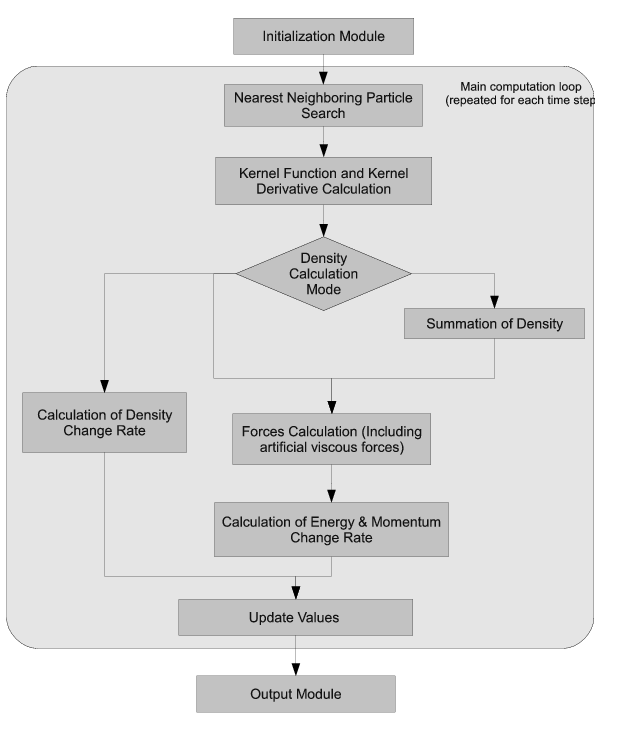
\includegraphics[width=1.0\textwidth]{Graphics/general_structure_SPH}
  \caption{Basic structure of an SPH code (adapted from \cite{Liu2003}) }
  \label{fig:BasicSphCode}
\end{figure}

\section{Presentation of test cases and porosity configurations}
\label{sec:GenIntroTestCases}
 
This section introduces the different test cases, which are used to validate the developed code at the different stages as well as the porosity configurations simulated once the code is validated. The general setup is presented for each problem. In addition, for the test cases,  analytical solutions are introduced in case they exist. Otherwise a numerical reference solution is provided.

The reason why this section is placed already here is, that the test problems are sometimes referred to from the code section (\ref{sec:1DSPHcode}),(\ref{sec:2DSPHcode}) and it is preferable if they are introduced before.

Details on initializing the flow--field, running the simulations and post--processing are not given in this section but only in section (\ref{sec:simuSetupTestCases}), after having introduced the numerical codes. The present section just provides the basics by introducing equations and the general ideas necessary to perform the actual simulation and the post-processing.

\subsection{1D shock--tube}
\label{sec:TestCases_1DshockTube}
As an exact solution is known, the 1D shock-tube is a very common test--case for compressible numerical techniques, especially in the form used by Sod \cite{Sod1978}.

%\subsubsection{Presentation and analytical solution}
 The problem consists of two initially separated (e.\ g.\ by a diaphragm) gas--filled tube sections, both in general with different properties, at least different pressure. When at the instant $t_0$ (initial situation shown in figure (\ref{fig:shockTubeT0})) the separation is removed, a shock wave is propagating into the low--pressure area and a rarefaction is traveling into the high pressure area, both adjusting the pressure to the same intermediate value. This means that at a time $t_1>t_0$ the situation can be presented as in figure (\ref{fig:shockTubeT1}) where the nomenclature from Anderson \cite{Anderson2002} is adopted.

\begin{figure}[h]
    \centering
\label{fig:shockTube}
\subfigure[Shock--tube at initial time $t_0$]{
      %\resizebox{!}{4cm}{% Generated with LaTeXDraw 2.0.8
% Tue Aug 31 14:18:55 PDT 2010
% \usepackage[usenames,dvipsnames]{pstricks}
% \usepackage{epsfig}
% \usepackage{pst-grad} % For gradients
% \usepackage{pst-plot} % For axes
\scalebox{1} % Change this value to rescale the drawing.
{
\begin{pspicture}(0,-1.7167188)(12.2,1.7567188)
\psframe[linewidth=0.04,dimen=outer](12.2,0.7032812)(0.0,-1.7167188)
\usefont{T1}{ppl}{m}{n}
\rput(1.775625,-0.51171875){\pscirclebox[linewidth=0.04]{4}}
\usefont{T1}{ppl}{m}{n}
\rput(10.318125,-0.49171874){\pscirclebox[linewidth=0.04]{1}}
\psline[linewidth=0.04cm](6.18,0.68328124)(6.18,-1.6767187)
\psline[linewidth=0.05cm,linestyle=dashed,dash=0.16cm 0.16cm,arrowsize=0.05291667cm 3.0,arrowlength=1.65,arrowinset=0.0]{<-}(6.2,-0.77671874)(7.36,1.0632813)
\usefont{T1}{ppl}{m}{n}
\rput(7.9,1.4082812){\psframebox[linewidth=0.04,framesep=0.1]{diaphragm}}
\usefont{T1}{ppl}{m}{n}
\rput(1.9523437,0.38828126){high pressure section}
\usefont{T1}{ppl}{m}{n}
\rput(10.131719,0.40828124){low pressure section}
\end{pspicture} 
}

}
      % Generated with LaTeXDraw 2.0.8
% Tue Aug 31 14:18:55 PDT 2010
% \usepackage[usenames,dvipsnames]{pstricks}
% \usepackage{epsfig}
% \usepackage{pst-grad} % For gradients
% \usepackage{pst-plot} % For axes
\scalebox{1} % Change this value to rescale the drawing.
{
\begin{pspicture}(0,-1.7167188)(12.2,1.7567188)
\psframe[linewidth=0.04,dimen=outer](12.2,0.7032812)(0.0,-1.7167188)
\usefont{T1}{ppl}{m}{n}
\rput(1.775625,-0.51171875){\pscirclebox[linewidth=0.04]{4}}
\usefont{T1}{ppl}{m}{n}
\rput(10.318125,-0.49171874){\pscirclebox[linewidth=0.04]{1}}
\psline[linewidth=0.04cm](6.18,0.68328124)(6.18,-1.6767187)
\psline[linewidth=0.05cm,linestyle=dashed,dash=0.16cm 0.16cm,arrowsize=0.05291667cm 3.0,arrowlength=1.65,arrowinset=0.0]{<-}(6.2,-0.77671874)(7.36,1.0632813)
\usefont{T1}{ppl}{m}{n}
\rput(7.9,1.4082812){\psframebox[linewidth=0.04,framesep=0.1]{diaphragm}}
\usefont{T1}{ppl}{m}{n}
\rput(1.9523437,0.38828126){high pressure section}
\usefont{T1}{ppl}{m}{n}
\rput(10.131719,0.40828124){low pressure section}
\end{pspicture} 
}

      
      \label{fig:shockTubeT0}
}
\subfigure[Shock--tube at time $t_1>t_0$]{
      % Generated with LaTeXDraw 2.0.8
% Tue Aug 31 14:32:35 PDT 2010
% \usepackage[usenames,dvipsnames]{pstricks}
% \usepackage{epsfig}
% \usepackage{pst-grad} % For gradients
% \usepackage{pst-plot} % For axes
\scalebox{1} % Change this value to rescale the drawing.
{
\begin{pspicture}(0,-1.21)(12.2,1.21)
\psframe[linewidth=0.04,dimen=outer](12.2,1.21)(0.0,-1.21)
\usefont{T1}{ppl}{m}{n}
\rput(1.775625,-0.005){\pscirclebox[linewidth=0.04]{4}}
\usefont{T1}{ppl}{m}{n}
\rput(10.318125,0.035){\pscirclebox[linewidth=0.04]{1}}
\psline[linewidth=0.04cm,linestyle=dashed,dash=0.16cm 0.16cm](6.48,1.11)(6.48,-1.15)
\psline[linewidth=0.04cm](8.7,1.17)(8.7,-1.19)
\usefont{T1}{ppl}{m}{n}
\rput(5.3664064,0.015){\pscirclebox[linewidth=0.04]{3}}
\usefont{T1}{ppl}{m}{n}
\rput(7.5034375,-0.005){\pscirclebox[linewidth=0.04]{2}}
\psline[linewidth=0.02cm](4.5,1.19)(4.5,-1.17)
\psline[linewidth=0.02cm](4.56,1.17)(4.56,-1.19)
\psline[linewidth=0.02cm](4.62,1.19)(4.62,-1.17)
\psline[linewidth=0.02cm](4.68,1.17)(4.68,-1.19)
\end{pspicture} 
}


      \label{fig:shockTubeT1}
}
\caption[Schematic of a shock--tube problem]{Situation in a shock--tube. \subref{fig:shockTubeT0} at the initial state, \subref{fig:shockTubeT1} after the separation of the two areas has been removed.}
\end{figure}

% \begin{figure}[h]
%     \centering
% \subfigure[Shock--tube at initial time $t_0$]{
%       %\resizebox{!}{4cm}{% Generated with LaTeXDraw 2.0.8
% Tue Aug 31 14:18:55 PDT 2010
% \usepackage[usenames,dvipsnames]{pstricks}
% \usepackage{epsfig}
% \usepackage{pst-grad} % For gradients
% \usepackage{pst-plot} % For axes
\scalebox{1} % Change this value to rescale the drawing.
{
\begin{pspicture}(0,-1.7167188)(12.2,1.7567188)
\psframe[linewidth=0.04,dimen=outer](12.2,0.7032812)(0.0,-1.7167188)
\usefont{T1}{ppl}{m}{n}
\rput(1.775625,-0.51171875){\pscirclebox[linewidth=0.04]{4}}
\usefont{T1}{ppl}{m}{n}
\rput(10.318125,-0.49171874){\pscirclebox[linewidth=0.04]{1}}
\psline[linewidth=0.04cm](6.18,0.68328124)(6.18,-1.6767187)
\psline[linewidth=0.05cm,linestyle=dashed,dash=0.16cm 0.16cm,arrowsize=0.05291667cm 3.0,arrowlength=1.65,arrowinset=0.0]{<-}(6.2,-0.77671874)(7.36,1.0632813)
\usefont{T1}{ppl}{m}{n}
\rput(7.9,1.4082812){\psframebox[linewidth=0.04,framesep=0.1]{diaphragm}}
\usefont{T1}{ppl}{m}{n}
\rput(1.9523437,0.38828126){high pressure section}
\usefont{T1}{ppl}{m}{n}
\rput(10.131719,0.40828124){low pressure section}
\end{pspicture} 
}

}
%       % Generated with LaTeXDraw 2.0.8
% Tue Aug 31 14:18:55 PDT 2010
% \usepackage[usenames,dvipsnames]{pstricks}
% \usepackage{epsfig}
% \usepackage{pst-grad} % For gradients
% \usepackage{pst-plot} % For axes
\scalebox{1} % Change this value to rescale the drawing.
{
\begin{pspicture}(0,-1.7167188)(12.2,1.7567188)
\psframe[linewidth=0.04,dimen=outer](12.2,0.7032812)(0.0,-1.7167188)
\usefont{T1}{ppl}{m}{n}
\rput(1.775625,-0.51171875){\pscirclebox[linewidth=0.04]{4}}
\usefont{T1}{ppl}{m}{n}
\rput(10.318125,-0.49171874){\pscirclebox[linewidth=0.04]{1}}
\psline[linewidth=0.04cm](6.18,0.68328124)(6.18,-1.6767187)
\psline[linewidth=0.05cm,linestyle=dashed,dash=0.16cm 0.16cm,arrowsize=0.05291667cm 3.0,arrowlength=1.65,arrowinset=0.0]{<-}(6.2,-0.77671874)(7.36,1.0632813)
\usefont{T1}{ppl}{m}{n}
\rput(7.9,1.4082812){\psframebox[linewidth=0.04,framesep=0.1]{diaphragm}}
\usefont{T1}{ppl}{m}{n}
\rput(1.9523437,0.38828126){high pressure section}
\usefont{T1}{ppl}{m}{n}
\rput(10.131719,0.40828124){low pressure section}
\end{pspicture} 
}

      
%       \caption{Shock--tube at initial time $t_0$}
%       \label{fig:shockTubeT0}
% \vspace*{0.3cm}
%       % Generated with LaTeXDraw 2.0.8
% Tue Aug 31 14:32:35 PDT 2010
% \usepackage[usenames,dvipsnames]{pstricks}
% \usepackage{epsfig}
% \usepackage{pst-grad} % For gradients
% \usepackage{pst-plot} % For axes
\scalebox{1} % Change this value to rescale the drawing.
{
\begin{pspicture}(0,-1.21)(12.2,1.21)
\psframe[linewidth=0.04,dimen=outer](12.2,1.21)(0.0,-1.21)
\usefont{T1}{ppl}{m}{n}
\rput(1.775625,-0.005){\pscirclebox[linewidth=0.04]{4}}
\usefont{T1}{ppl}{m}{n}
\rput(10.318125,0.035){\pscirclebox[linewidth=0.04]{1}}
\psline[linewidth=0.04cm,linestyle=dashed,dash=0.16cm 0.16cm](6.48,1.11)(6.48,-1.15)
\psline[linewidth=0.04cm](8.7,1.17)(8.7,-1.19)
\usefont{T1}{ppl}{m}{n}
\rput(5.3664064,0.015){\pscirclebox[linewidth=0.04]{3}}
\usefont{T1}{ppl}{m}{n}
\rput(7.5034375,-0.005){\pscirclebox[linewidth=0.04]{2}}
\psline[linewidth=0.02cm](4.5,1.19)(4.5,-1.17)
\psline[linewidth=0.02cm](4.56,1.17)(4.56,-1.19)
\psline[linewidth=0.02cm](4.62,1.19)(4.62,-1.17)
\psline[linewidth=0.02cm](4.68,1.17)(4.68,-1.19)
\end{pspicture} 
}


%       \caption{Shock--tube at time $t_1>t_0$}
%       \label{fig:shockTubeT1}
% \end{figure}

In figure (\ref{fig:shockTubeT1}), areas 2 and 3 are separated by the so called contact discontinuity, which is the fluid interface generated by the removal of the diaphragm. While in general, the states and properties of the fluids in 2 and 3 are different, pressure $p$ and velocity $u$ at both sides of the discontinuity have to be the same:
\begin{equation}
\begin{split}
\label{eq:condCD}
p_2&=p_3\\
u_3&=u_2
\end{split}
\end{equation}

The analytical solution to the shock--tube problem can be found using the shock relations and the isentropic relations and is taken from Anderson \cite{Anderson2002} as well. 
It will be presented here, as the post--processing described in section (\ref{sec:2Dshock_simuSetup&Co}) is based on this solution.

First the unknown quantities in areas 2 and 3 are calculated (states 1 and 4 are completely known). Then the location of all area boundaries is determined at a certain instant $t_1>t_0$. Finally the properties inside the rarefaction (located between area 3 and 4) can be obtained.

\paragraph{Determination of quantities in areas 2 and 3}

With the relation

\begin{equation}
 \frac{p_4}{p_1} = \frac{p_2}{p_1}  \left(1-\frac{(\gamma_4-1)\frac{c_1}{c_4}\left(\frac{p_2}{p_1}-1\right)}{\sqrt{2\gamma_1\left(2 \gamma_1+(\gamma_1+1)\left(\frac{p_2}{p_1}-1\right)\right)}}\right)^{\left(\frac{-2 \gamma_4}{\gamma_4-1}\right)}
\end{equation}
the unknown pressure $p_2$ can be determined iteratively, where the sound speed for an ideal gas is calculated according to equation (\ref{eq:soundSpeed}). 

For the further proceeding, the ratio of specific heats $\gamma$ is assumed constant (i.\ e.\ same gas in 1 and 4 and besides no variation of $\gamma$ with temperature)

\begin{equation}
 \gamma_4= \gamma_3= \gamma_2= \gamma_1=const.
\end{equation}
The density in area 2 can be determined from state 1 with the shock relations 
\begin{equation}
 \rho_2=\rho_1\frac{1+\frac{\gamma+1}{\gamma-1}\frac{p_2}{p_1}}{\frac{\gamma+1}{\gamma-1}+\frac{p_2}{p_1}}.
\end{equation}
Applying the isentropic relations from state 4, one obtains the density in area 3
\begin{equation}
\rho_3=\left(\frac{p_3}{p_4}\right)^{\frac{1}{\gamma}}\rho_4.
\end{equation}
The internal energy in areas 2 and 3 is obtained by the ideal gas equation of state (\ref{eq:idealGasEqState}).
The velocity of the shock traveling into area 1 is
\begin{equation}
\label{eq:shockVelocity}
U_s=c_1\sqrt{\frac{\gamma+1}{2\gamma}\left(\frac{p_2}{p_1}-1\right)+1}.
\end{equation}
With the application of the continuity equation, the velocity induced in area 2 $u_2$ by the shock is
\begin{equation}
 u_2=U_s\left(1-\frac{\rho_1}{\rho_2}\right).
\end{equation}
According to equation (\ref{eq:condCD}), the velocity in area 3 $u_3$ is the same.

\paragraph{Determination of the area boundaries at a certain instant}

As geometrical information comes into play, the position of the diaphragm in the space has to be indicated and is assumed to be $x_{dia}=0$ and $x$ is counted positively towards the right, i.\ e.\ in direction of the low pressure area (area 1).
The following positions have to be determined (see also figure (\ref{fig:shockTubeT1})):

\begin{itemize} 

  \item Begin rarefaction (delimits area 4): \\
As the begin of the rarefaction propagates into area 4 with the corresponding (local) sound speed, its position is 
\begin{equation}
 x_{rar,beg}=-c_4 t
\end{equation}

  \item End rarefaction (delimits area 3): \\
The end of the rarefaction propagates with the corresponding (local) sound speed relative to the fluid in 3 which itself has a velocity $u_3$. The desired position is therefore
\begin{equation}
 x_{rar,end}=(u_3-c_3) t
\end{equation}

  \item Contact discontinuity: \\
The contact discontinuity moves with the velocity $u_3$ and therefore
\begin{equation}
 x_{CD}=u_3 t
\end{equation}

  \item Shock: \\
  The expression for the propagation velocity $W$ is given by equation (\ref{eq:shockVelocity}) and therefore
\begin{equation}
 x_{shock}=W t
\end{equation}

\end{itemize}

\paragraph{Determination of the properties inside the rarefaction}
Inside the rarefaction the flow evolves in an isentropic manner, which means the isentropic relations can be employed. Furthermore, the theory of characteristics gives the velocity at a certain point inside the rarefaction. Again all equations are taken from Anderson \cite{Anderson2002} and the coordinate system remains unchanged. $x=0$ corresponds to the diaphragm position and therefore is the origin of the rarefaction.

To obtain the velocity inside the rarefaction, the following equation is used
\begin{equation}
 u_{rar}=\frac{2}{\gamma+1}\left(c_4+\frac{x}{t}\right)
\end{equation}
\noindent
The density at a certain point inside the rarefaction is calculated with
\begin{equation}
\rho=\rho_4 \left(1-\frac{\gamma-1}{2}\frac{u}{a_4}\right)^\frac{2}{\gamma-1}
\end{equation}
and for the pressure, the isentropic relation in the following form is used
\begin{equation}
p=p_4\left(\frac{\rho}{\rho_4}\right)^\gamma
\end{equation}
Finally, the internal energy is computed with the equation of state (\ref{eq:idealGasEqState}).

\subsection{Acoustic wave propagation}
\label{sec:AcousticWavePropagation_GenIntro}
Acoustic phenomena play an important role for the actual problem to be investigated within this project (see chapter (\ref{sec:intro})). It is therefore necessary to get an idea on how the code reproduces these phenomena. A crucial issue in this context is the damping of oscillating or propagating waves due to numerical dissipation: many numerical codes have an intrinsic dissipation, introduced by the numerical scheme, even when the actually implemented equations are inviscid. This numerical dissipation acts like a real viscous dissipation and diminishes the kinetic energy of the flow. The comparison of the simulation results against the following test cases, whose theoretical solution is always obtained assuming an inviscid flow (i.\ e.\ no dissipation), aim at quantifying this damping. A further point to be investigated by means of these test cases is the capability of the code to exactly reproduce the right periodical time $T$ of the propagating or oscillating wave.

Note: in this section, $T$ denotes not the temperature, but the periodical time. 

%%%%%%%%%%%%%%%%%%%%%%%%%%%%%%%%%%%
%SPH without art. viscosity. does not show any (numerical) damping at all,
% can this be explained somehow by the nature of the method?
%it does not have anything to do with the conservation properties of the method, right???
%momentum conservation: as long as EXTERNAL forces=0 momentum conserved
% and dissipation is internal force...
%energy conservation: dissipation transforms energy from kinetic to thermal
% so energy is conserved for dissipation processes logically...
 
In order to quantify the effect of viscosity in the simulation results (no matter what nature it is), a damping factor
is introduced as the relative change in amplitude $A$ of two consecutive periods $i$ and $i+1$
\begin{equation}
\label{eq:DampingFactor}
 f_d=\frac{A_i-A_{i+1}}{A_i}
\end{equation}
where the amplitude $A$ may be measured either in terms of pressure $p$ or velocity $u$.

%For the case of a damping force that is proportional to the velocity, the damping factor is constant. This fact is important with regard to the artificial viscosity that can be included in the code (see section (\ref{sec:ArtVisc})). A closer look at the formulation for the artificial viscosity (equation (\ref{eq:MonArtVis})) yields
% \begin{equation}
%  \Pi_{ab}\propto u_{ab}.
% \end{equation}
% This above statement is made assuming $\nu$ from equation (\ref{eq:MonArtVis}) constant.
%%% WHICH IS actually not at all true, see openoffice-sheet etc.\\..
%%% so, how comes that the damping--factor is constant although the repelling force is not propto the velocity???
%%% am i thinking the wrong way???

%%or perhaps: mue has always about the same value (although globally variable as art. visc. depends on compression/expansion) in the areas where damping occurs (in the compression/expansion zones of the waves) and so, the above statement PI propto velocity is about right
An alternative way of assessing the damping is for example used by \cite{Attwood2007} and consists of analyzing the decay in total kinetic energy of the wave. However this approach is not used here. 



\subsubsection{1D stationary oscillating wave}
The configuration of an oscillating wave is taken from \cite{Monaghan2005}, where it is used to study the dispersion relation for an infinite one--dimensional gas. In the present context though, the same configuration is judged suitable for the study of damping and evolution of the periodical time $T$.

The sinusoidal oscillation of wavelength $\lambda$ is generated by a velocity profile with amplitude of 5\% of sound speed
\begin{equation}
\label{eq:InitialVelocityPerturbationOscillatingWave}
 u(x)=0.05 c\sin\left(\frac{2\pi x}{\lambda}\right)
\end{equation}
in the domain $0\leq x\leq \lambda$ with periodical boundary conditions on both sides.

For a simple harmonic wave, the theoretical periodical time $T$ is given as \cite{Stewart1930}
\begin{equation}
 T=\frac{\lambda}{c}
\end{equation}
and serves as a reference for the comparison with the simulation results.





\subsubsection{1D infinite traveling wave}
This test case is similar to the above one with the difference that now the wave travels in one direction through the space. A theoretical description for this kind of wave can be found using the wave equation for a velocity potential. This is a linearized equation and therefore valid only for small disturbances, which for the present application is justified. In Stewart \cite{Stewart1930}, the expressions for the fluctuation (denoted by $\delta$) of the desired quantities around their mean values (denoted by the subscript $0$) are explicitly given and read as follows:
\begin{itemize}
\item velocity evolution 
\begin{equation}
\label{eq:1DWaveDetla_u}
 \delta u(x,t)=k A' \sin(k(ct-x))
\end{equation}
\item density evolution 
\begin{equation}
 \delta \rho(x,t)=\rho_0\frac{k}{c} A'  \sin(k(ct-x))
\end{equation}
\item pressure evolution 
\begin{equation}
 \delta p(x,t)=k c \rho_0 A'  \sin(k(ct-x))
\end{equation}
\item evolution of the displacement $\xi=x-x_0$
\begin{equation}
\label{eq:1DWaveDisplacement}
 \xi(x,t)=-\frac{A' }{c} \cos(k(ct-x))=-\frac{A' }{c} \sin\left(k\left(ct-x+\frac{\pi}{2k}\right)\right)
\end{equation}

\end{itemize}

$A'$ denotes the amplitude of the underlying velocity potential and therefore determines the amplitude of the other quantities as well. It can be any random constant with the restriction that the disturbances in $\rho$ and $p$ remain small compared to their mean value (linear theory). The variable $k$ is the  wave number and defined as $k=\frac{2\pi}{\lambda}$.

Furthermore one can note that the displacement is $\pi/2$ or $90^\circ$ in phase ahead of the other quantities. This fact will be important when thinking about the initialization of a finite propagating wave (single wave train). 

For the initialization of the flow field at the instant $t=0$, the above equations (\ref{eq:1DWaveDetla_u})-(\ref{eq:1DWaveDisplacement}) will be employed (see section (\ref{sec:simuSetupTestCases})).
%%specify exact reference as soon as 1D Wave simu setup is written


\subsubsection{1D wave train with reflection and interference}
\label{sec:GenIntro_1DWaveTrainReflect}
For the testing of reflection and interference, the problem as described below is simulated.

But first, some thoughts on the initialization of a single 1D wave train are presented.
The Goal is to initialize a 1D wave train in one part of the domain while the rest shall be initialized with unperturbed flow. %For this to make any sense, the size of the domain has of course to be superior to the wavelength $\lambda$ of the wave train. 

First attempts to initialize the single wave train using the equations for a continuous (infinite) traveling wave (\ref{eq:1DWaveDetla_u})-(\ref{eq:1DWaveDisplacement}) have turned out to be problematic due to the phase shift between $\rho,p,u$ on the one hand and the displacement $\xi$ on the other hand. As the wave does not continue infinitely but is simply cut off after one wavelength, there will always be a discontinuity in one of the quantities.  

If, for example, the initialization is done with a smooth transition of $\rho,p,u$ from the unperturbed flow, there is a discontinuity in the displacement, and vice versa. This discontinuity (be it in $\rho,p,u$ or in the displacement) constitutes a new disturbance which again is origin of new waves. So, no neat wave train could be created this way. 
Thus, a different way to generate the wave had to be found and it turned out that the periodic movement of a wall boundary was an appropriate mean to do so. 

Now that single wave trains can be produced, the test case is introduced:
A 1D domain with size $l_{\mathit{dom}}$ and limited by two solid walls (at $x=0$ and $x=l_{\mathit{dom}}$) is considered. The left hand wall at $x=0$ has the ability to perform a movement according to a sinusoidal velocity profile, when desired.
The periodical time $T$ of the wave train is chosen in a way that its wavelength is
$\lambda=l_{\mathit{dom}}/4$. The condition on $T$ is therefore
\begin{equation}
 T=\frac{l_{\mathit{dom}}}{4 c_0}.
\end{equation}

The following passage explains the temporal course of the theoretically exact test problem

\begin{itemize} 
\item At $t_0=0$ the left hand side wall begins to move according to 
\begin{equation}
  u_{\mathit{wall}}=u_{\mathit{max}}\sin(\omega t) 
\end{equation}
  where $\omega=\frac{2\pi}{T}$ and $u_{\mathit{max}}=0.05 c_0$.


\item At $t_1=T$ the wall stops moving, meaning that exactly one wave train has been generated, which now travels through the domain.

\item At $t_2=l_{\mathit{dom}}/c_0$ the first part of the wave train hits the right hand side  wall and starts being reflected. Simultaneously, the LHS wall starts moving again according to same equation as above, generating a new wave.

\item At $t_3=t_2+T$ the LHS wall stops moving and the generation of the second wave is finished. 
The first wave is now completely reflected from the RHS wall.

\item At $t_4=t_3+T$ the two waves begin to interfere (both wave trains reach the center of the domain).

\item At $t_5=t_4+T/2$ the interference of the waves is at maximum, i.\ e.\ both waves interfere along their entire wavelength.

\item At $t_6=t_4+T$ the wave interference is over.

\item At $t_7=t_6+T$ both waves hit the respective walls. The test problem ends at this instant.
\end{itemize}


%To get a visual idea of this problem, refer to figure LABEL (show to situations with wave trains...)

\subsection{Taylor--Green flow}
\label{sec:GenIntro_TG}
The Taylor--Green flow is an appropriate test case to verify the viscosity implementation. As the problem consists of an infinite 2D domain, it can numerically be realized by periodical boundary conditions and viscosity can be tested without any interference of no--slip solid wall boundary conditions. The latter are an issue for SPH and are therefore tested separately by means of a Poiseuille test--case (see section (\ref{sec:genIntroPoiseuille})).
The Taylor--Green flow consists of a periodical arrangement of vortices in the way shown in figure (\ref{fig:GeneralSitu_TG}).
\begin{figure}
 \centering

\label{fig:GeneralSitu_TG}
%\includegraphics[]{}
\caption[Taylor--Green flow general presentation]{Initial situation of a Taylor--Green flow}
\end{figure}

An analytical expression for the temporal evolution of the velocity field of the incompressible 2D Taylor--Green flow is given by \cite{Chaniotis2002}
\begin{equation}
 \label{eq:TG_analyticalSolution}
\begin{split}
u_x(x,y,t)&=-U_0 e^{bt}\cos(2\pi x)\sin(2\pi y)\\
u_y(x,y,t)&=U_0 e^{bt}\sin(2\pi x)\cos(2\pi y)
\end{split}
\end{equation}
with $b=\frac{-8\pi^2}{Re}$ characterizing the temporal decay of the velocity field. The Reynolds number is defined for this case as $Re=\frac{\rho U_0 l_\mathit{char}}{\eta}$.


\subsection{Pure heat--conduction -- Slab with temperature jump}
\label{sec:genIntro_PureHeat}
The configuration used to test the thermal conduction is a solid slab with an initial temperature jump. The LHS is initially at low temperature, the RHS at high temperature. A configuration with adiabatic boundary conditions at the domain edge is investigated as well as one with isothermal boundary conditions.

For this configuration, the temporal evolution of the temperature field in the initial phase can be described by the analytical solution of two semi infinite solids with same thermal conductivity $k$, same density $\rho$ and same heat capacity $c$ %(here: $c=c_v$ as code actually for fluids). 
The following equations are for a situation where the LHS ($x \leq x_m$) of the slab is at $T_l=0$ and RHS ($x > x_m$) at $T_r=const.$ \cite{Carslaw1959}.
\begin{equation}
\label{eq:Two_SemiInfBodies}
 T(x,t)=\begin{cases}
\frac{1}{2} T_r erfc\left(\frac{|x-x_m|}{2\sqrt{\alpha t}}\right),& \text{for  $x\leq x_m$} \\
\frac{1}{2} T_r\left(1+erf\left(\frac{x-x_m}{2\sqrt{\alpha t}}\right)\right),& \text{for  $x> x_m$}
\end{cases}
\end{equation}
where $\alpha=\frac{k}{\rho c}$ is called the thermal diffusivity. 



\subsection{Compressible Couette flow}
\label{sec:comprCouette_genIntro}
A Couette flow in general designates a flow that originates in the following situation: a viscous fluid between two infinite parallel plates of distance $d$ is originally at rest. At the instant $t=0$ one of the plates starts moving with a constant velocity $u_p$ dragging the flow along with it. Furthermore the two plates may also have different temperatures. After a certain time a steady state solution establishes. 

To characterize the influence of the viscous forces, the Reynolds number for the Couette configuration is defined as
\begin{equation}
\label{eq:Re_comprCouette}
 Re=\frac{\rho u_p d}{\eta}
\end{equation}.

In the case where the velocity $u_p$ is small enough and where besides the wall temperatures are close enough together (ideally both the same and equal to the initial fluid temperature), the flow can be considered incompressible with $\rho=const.$ which also implies the assumption of $T=const$. and therefore $\eta=const.$ and $k=const.$. The steady state solution in this case consists therefore of a linear velocity profile between the plates (out of the condition that the viscous shear stress $\tau$ needs to be constant over the canal).

In the case, however, where the plate velocity $u_p$ is that big, that the viscous dissipation is not negligible any more or where the wall temperatures are too different from the flow temperature, there will be a considerable temperature gradient in the flow implying that $\rho$,$\eta$ and $k$ now have to be considered variable. This situation is then called a compressible Couette flow which is of interest as a test case in the present work.
The steady state velocity profile for the compressible Couette is not linear anymore but is affected by the non-constant viscosity. As the condition $\tau(y)=const.$ does still apply for the steady state, the velocity gradient at a certain position $y$ evolves inversely to the local viscosity value, according to the equation for the shear stress $\tau=\eta \frac{\partial u}{\partial y}$ \cite{Anderson2001}. 
An analogous consideration for the steady state temperature profile can principally be made. The corresponding condition of constant heat flux in the transverse canal direction however only applies when neglecting the heat produced by viscous dissipation. 


\subsection{Poiseuille flow}
\label{sec:genIntroPoiseuille}
The flow models themselves already being tested by all the above cases, the Poiseuille flow is primarily used to test the no--slip boundary conditions. 

A Poiseuille flow consists of a flow in a canal of infinite length in one dimension, in this case the x--direction. The canal is confined  in the transverse direction (y--direction) by two walls, which here have a distance of $2d$. The fluid in this canal is initially at rest and for $t\geq0$ a pressure gradient in x--direction $\partial p/\partial x $ or equivalent a body force (force per unit mass) of value $g=\frac{1}{\rho}{\delta p}{\delta x}$ \cite{Sigalotti2003} in the same direction are applied and lead to the evolution of a flow. The incompressible steady state solution of this flow is a parabolic profile of the velocity in x--direction and given by \cite{Sigalotti2003} as
%something wrong with \cite{Basa2009}-equation, better ref is \cite{Sigalotti2003}.
\begin{equation}
\label{eq:Poiseuille_steadyState_U}
 u(y,t=\infty)=\frac{g \rho}{2 \eta}(d^2-y^2)
\end{equation}
The origin of the coordinate system ($y=0$) is supposed at the center line of the canal.
A theoretical solution for the temporal evolution of the (incompressible) Poiseuille velocity profile is given by \cite{Sigalotti2003}
\begin{equation}
\label{eq:Poiseuille_Series}
 u(y,t)=1-\frac{32}{\pi^3}\left(\frac{y}{d}\right)^2 -\sum_{n=0}^\infty \frac{16(-1)^n d^2 g \rho}{eta \pi^3 (2 n +1)^3}\cos \left(\frac{(2n+1)\pi y}{2 d} \right)\exp \left(- \frac{(2n+1)^2\pi^2\eta t}{4d^2\rho} \right).
\end{equation}
 

\subsection{Semi--infinite body}
\label{sec:genIntroSemiInfBody}
The analytical solution of a semi--infinite body with isothermal boundary condition can be used as a reference solution for the test of the isothermal boundary implementation is section (\ref{sec:TestSolobs_BC}).
A semi infinite body with constant initial temperature $T_0$  and a constant temperature boundary condition at the edge ($T_w$) has the temperature field \cite{Carslaw1959}
\begin{equation}
\label{eq:SemiInfBodySolution}
 T(x,t)=T_w+erf \left(\frac{x}{2 \sqrt{at}} \right) \left(T_0-T_w \right).
\end{equation}


\subsection{Porosities -- Cavities}
\label{sec:Porosities_Cavity}
The configuration of a sequence of cavities in a linear wall as shown in figure (\ref{fig:SequanceOfCavities}) is a 2D approximation to the situation in the experimental setup for the high enthalpy flow over a slender cone with porous walls. For, in the experiment the porous wall surface consists of a high number of little dead holes or cavities.

\begin{figure}[!htbp]
  \centering
     %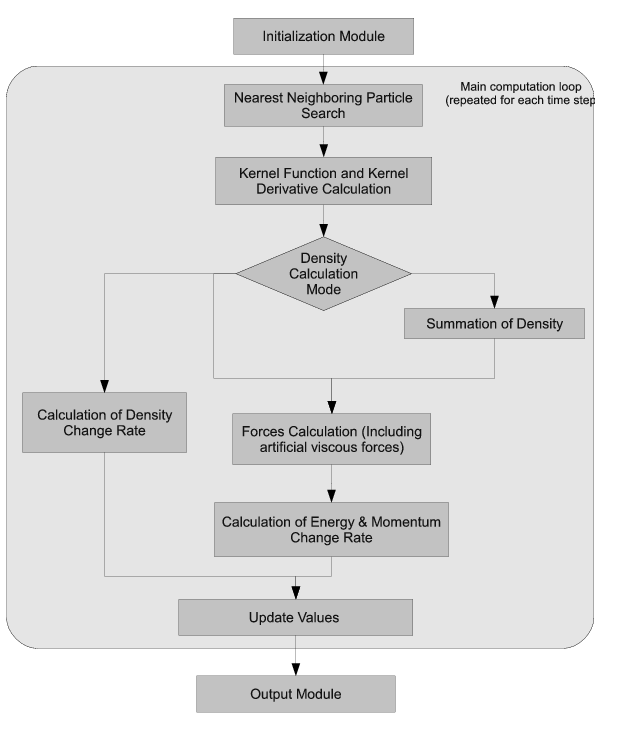
\includegraphics[width=1.0\textwidth]{Graphics/general_structure_SPH}
  \caption{A sequence of cavities: Hier eine ganze reihe von cavities reinmachen und randbedingungen erst un SIumsetup darstellen }
  \label{fig:PorositiesSequenceOfCavities}
\end{figure}


\subsection{Porosities -- flow through circular obstacles}
\label{sec:PorositiesCircularObstacles}
A further investigated 2D porosity configuration is the one of a flow through circular obstacles arranged in a rectangular lattice as illustrated in figure (\ref{}). To take advantage of the ability of the code to treat heat conduction and compressible flows, a hot flow, cold wall situation will be examined. The present porosity configuration is in no direct link with the underlying experimental setup, but it constitutes an interesting setup and thus was considered worth an investigation in this project. 

\begin{figure}[!htbp]
  \centering
     %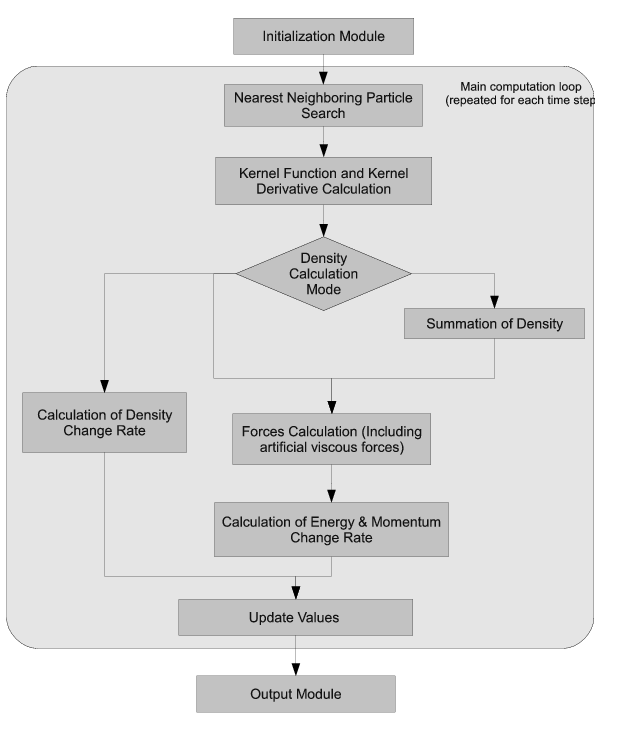
\includegraphics[width=1.0\textwidth]{Graphics/general_structure_SPH}
  \caption{A porous media as used for porosity simulation: Hier eine ganze reihe von obstacles reinmachen und randbedingungen erst un SIumsetup darstellen }
  \label{fig:PorositiesCircularObstacles}
\end{figure}


\section{1D SPH code}
\label{sec:1DSPHcode}

\subsection{Short overview}
%PERHAPS THIS SUBSECTION TITLE IS REMOVED AND THE FOLLOWING TEXT WILL FIGURE JUST BELOW THE SECTION TITLE!?!

This code has a relatively simple structure, yet it features all the components
a more sophisticated SPH computational program would incorporate and incorporates the SPH formulations of the Euler equations. The nearest neighbor particle search is conducted with the simple all pair search allgorihm with pairwise interactions (section \ref{sec:NNPS}), meaning at the same time that the smoothing length remains constant. The above introducted cubic spline kernel serves as smoothing function (setion (\ref{sec:KernelFunction})) and temporal integration is conducted with the leap--frog allgorithm (section \ref{sec:numIntegr}) and a constant manually chosen timestep. As the code simulates a problem including shocks, the Monaghan artificial viscosity is integrated (section \ref{sec:ArtVisc})).Finally, both the summation density approach and the continuity density approach are implemented (see section (\ref{sec:DensCalcMode})). 
By computing a 1D shock--tube problem, the code is used to verify the the basic compressible SPH Euler equations which are then implemented in the more complex 2D program. Beyond that, this code has no practical use. Nevertheless, it is presented herer as it facilitates a first understanding of the SPH implementation due to its simple structure.
  
%As the analytical solution for this problem is well known, the shock--tube is a very common test case for 1D compressible codes \cite{Sod1978}.
%(PERHAPS ONE MORE REFERENCE WHICH STATES THAT shock-tube IS A COMMONLY USED TEST CASE...). 
%The problem setup and the results obtained are discussed in the corresponding sections.

\subsection{Components and structure}
\label{sec:CompAndStruc1DCode}
%This section introduces all the...noch ergänzen

\subsubsection{The data structures}

To facilitate the implementation and the handling of the code, two data structures are defined. 

\paragraph{The {\tt parameters} data structure}

This data structure is defined in the header file {\tt parameters.h} and 
contains all parameters needed to set up the problem. Among those parameters are 
geometrical values, the initial conditions, simulation length and time step 
as well as parameters defining the fluid properties.

\paragraph{The {\tt simulation} data structure}

Defined in the file {\tt simulation.h}, this structure is made up of all 
variables that change in the course of the simulation. To begin with, these are the values of interest like position, velocity, density, pressure, energy, etc. Furthermore there are variables needed as intermediate results, such as the value of the smoothing function and its derivative for each interaction pair for example. 
Most of the variables contained in the simulation data structure are needed one per particle. Therefore those variables are defined as vectors with a size that corresponds to the number of particles in the domain. 

\subsubsection{The functions}

As the size of the 1D SPH program is not too big, it admits of the description of every single function used. The textual description is not complete but only comprises particularities and features that are considered worth mentioning. A Nassi-Schneidermann-Diagram (NSD)~\cite{Nassi1973} complements each description and shows the control flow for each function as well as the interdependence of the individual functions. For the sake of a clear illustration, the NSD does not display every loop of the program; frequently, loops over all particles and the interaction list are omitted. The instruction 'calculate for each particle' for example means at code level the implementation of a loop over all particles, i.\ e.\, all components of the corresponding variable's vector.  Consulting the comments in the source code is recommended if a more detailed understanding is desired.

\paragraph{Nassi-Schneidermann-Diagram -- a short introduction}
A NSD is employed in this section as it allows for a more compact description of the code structure within limited space than a conventional flow diagram and offers a range of further advantages~\cite{Nassi1973}. It is read from top to bottom, with different box symbols representing different kinds of instructions or control elements. The symbols used during the description of the functions below are the following ones:

\subparagraph{The process symbol:}

This symbol represents simple instructions for which during their execution no analysis has to be made. Examples are assignments or inputs/outputs. 
A variation of the conventional process box is the symbol for the call of an external function.
\begin{figure}
\centering
\subfigure[normal Instruction]{
\begin{struktogramm}(50,12)
  \assign[10]{\(instruction\)}
\end{struktogramm}
}
\subfigure[function call]{
\begin{struktogramm}(50,12)
  \sub[10]{\texttt{function()}}
\end{struktogramm}
}
\caption{The NSD process symbols }
\end{figure}

\subparagraph{The iteration symbol:}
The shown iteration symbol represents loops, where the condition is tested each time before entering the body. This control struct can be implemented by a while--loop or a for--loop. An example is shown in figure (\ref{NSD_whileLoop}).

\begin{figure}[H]
\centering
\label{NSD_whileLoop}
\begin{struktogramm}(50,22)
\while[10]{\(while \ condition \ true\)}  
\assign[10]{\(body\)}
\whileend
\end{struktogramm}

\caption{The NSD iteration symbol}
\end{figure}

\subparagraph{The decision symbols:}
Control structures that depending on a condition enter different branches are represented by the decision symbols. A binary decision symbol corresponding to an if-else statement in programming languages is shown in figure (\ref{fig:NSD_decision_binary}). For multi--branch control structs, such as if--elseif--else or switch--case, figure (\ref{fig:NSD_decision_multiple}) provides the corresponding symbol (in the example: 3 branches).
 
\begin{figure}[H]
\centering
\subfigure[binary decision]{
\label{fig:NSD_decision_binary}	
\begin{struktogramm}(50,22)
\ifthenelse[10]{6}{6}{\(condition \ true?\)}{Y}{N}
\assign[10]{\(subblock\ 1\)}
\change
\assign[10]{\(subblock\ 2\)}
\ifend
\end{struktogramm}
}
\subfigure[multiple decision]{
\label{fig:NSD_decision_multiple}	
\begin{struktogramm}(50,22)
  \case[10]{3}{3}{\(test\ X\ \ \ \ \ \ \ ~ \ \)}{\(cond. 1\)}
        \assign[10]{\(subblock\ 1\)}
    \switch{2}
        \assign[10]{\(subblock\ 2\)}
    \switch[r]{3~}
      \assign[10]{\(subblock\ 3\)}
   \caseend
\end{struktogramm}
}
\caption{The NSD decision symbols }
\end{figure}

Remark: The NSD flowchart language provides the possibility to describe programs at their level of implementation. In the following section however, it is used in a more abstract way and instructions or conditions are verbalized. 
 
\paragraph{The Main function}

As its name suggests, {\tt main.cpp} is the main function of the program. It is entered upon execution of the program, declares and initializes the data structures and calls the functions needed. Its structure is given in figure (\ref{fig:main_structure}).

\begin{figure}[H]
\label{fig:main_structure}
\begin{center}
\begin{struktogramm}(76,27)[MAIN]
  \assign{\(declare \ parameters\ data\ structure\)}
  \assign{\(declare \leq 4 \ simulation\ data\ structure\)}
  %\sub{\begin{verb} setupSim(param, sims) \end{verb}}
  \sub{\texttt{setupSim(param, sims)}}
  %\sub{\begin{verb} \ marchTime(param, sims)\end{verb}}
  \sub{\texttt{marchTime(param, sims)}}
  \assign{\(return\ 0  \ (program\ successfully\ ended)\)}
\end{struktogramm}
\end{center}

\caption{The structure of the main--function}
\end{figure}

\paragraph{The setupSim function}
\label{sec:1DSPHcode_functions_setupSim}

Implemented in the file {\tt setupSim.cpp} with the corresponding header {\tt setupSim.h}, this function represents the 'initialization module' shown in figure (\ref{fig:BasicSphCode}). More precisely, it first sets up the initial particle distribution for the shock--tube problem: depending on the user's selection made by setting the flag 'constspacing', which is a member of the {\tt parameters} data structure, this is done in two different ways:
\begin{itemize}
 \item 


 \item One possibility is to have an initial particle distribution with the same spacing in the high density area of the shock-tube as in the low density area (flag {\tt constspacing = true}). In this case though, the mass of the particles has then to be adapted to be coherent with the spacing and the initial value of the density.
 a\item A second possibility is a particle distribution resulting of a spatially constant particle mass (flag constspacing= false). According to the initial value of the density, the particles will then be further apart in the low density area than in the high density area.
\end{itemize}
For the further course of the program it is essential that each particle has a unique mean of identification. For more sophisticated 2D or 3D codes, this issue ican be resolved by explicitly assigning each particle an identification number. For this 1D code however, particle identification is already implicitly given due to the way, the particles and their information are stored: the position, consisting only of an $x$ value, of each particle is stored as one component of a position vector X. Therefore the particles can be clearly identified by the number of the vector component they are stored into.

Once the particles are set up, they are assigned their initial values for the shock-tube problem as chosen in the {\tt parameters.h} file.
\begin{figure}[H]
\label{fig:setupsim_structure}  
\begin{center}
\begin{struktogramm}(115,124)[SETUPSIM]
  \assign{\(calculate\ LHS \ particle\ spacing\ (dxl)\ based\ on\ constant\ mass\)}
  \assign{\(calculate\ RHS \ particle\ spacing\ (dxr)\ based\ on\ constant\ mass\)}
  \assign{\(calculate\ particle\ spacing\ (dx)\ for\ constant\ spacing\)}
  \ifthenelse[10]{6}{6}{\(constspacing\ flag==1?\)}{Y}{N}
    \assign[15]{\(place\ particles\ on\ LHS \ of \)\linebreak \( domain\ starting\ at\ center\ (x=0)\ ((with\ distance\ dx)\)}
    \assign[15]{\(place\ particles\ on\ RHS\ of\)\linebreak \( domain\ starting\ at\ x=0\ (with\ distance\ dx)\)}
  \change
    \assign[15]{\(place\ particles\ on\ LHS\ of\ \)\linebreak \( domain\ starting\ at\ x=0\ (with\ distance\ dxl)\)}
    \assign[15]{\(place\ particles\ on\ RHS\ of\ \)\linebreak \( domain\ starting\ at\ x=0\ (with\ distance\ dxr)\)}
  \ifend
  \assign{\(merge\ particle\ positions\ for\ both\ sides\ into\ one\ vector\ x\)}
  \assign{\(create\ vectors\ with\ initial\ values\ for\ u,\ \rho,\ p,\ e,\ m,\ h\ \)\linebreak \(for\ particles\ on\ LHS \)}
  \assign{\(create\ vectors\ with\ initial\ values\ for\ u,\ \rho,\ p,\ e,\ m,\ h\ \)\linebreak \(for\ particles\ on\ RHS \)}
  \assign{\(merge\ LHS\ and\ RHS\ vectors\ into\ single\ vector\ for\ each\ variable\)}
  \ifthenelse[10]{6}{1}{\(constspacing\ flag\ ==\ 1?\)}{Y}{N}
    \assign{\(calculate\ mass\ for\ particles\ on\ left\ hand\ side\)}
    \assign{\(calculate\ mass\ for\ particles\ on\ right\ hand\ side\)}
    \assign{\(merge\ mass\ values\ into\ one\ single\ vector\ \)\linebreak \((overwrite\ mass\ vector\ from\ above)\)}
  \change
  \ifend
  \assign{\(initialize\ vectors\ for\ derivatives\ \ du,\ de,\ d\rho \)}
\end{struktogramm}
\end{center}

\caption{The structure of the setupSim--function}
\end{figure}


\paragraph{The marchTime function}

The marchTime function conducts the numerical integration using the leapfrog scheme described in section (\ref{sec:numIntegr}). If the program runs in the continuity density mode (flag {\tt sumdensity = false}), the density is integrated as well, whereas if the program runs in the summation density mode ({\tt flag sumdensity = true}) the density is smoothed. The latter operation is not performed directly in this function but in one of the (sub)functions that it calls.

\begin{figure}[H]
\label{fig:MarchTime_structure}  

\begin{center}
% \sProofOn
     \begin{struktogramm}(115,134)[MARCHTIME]
  \assign{\(initialize\ vectors\ for\ intermediate\ values\ of\  \rho,\ u,\ e\)}
  \while[10]{\(while\ current\ time\ step\ \leq \ number\ of\ total\ time\ steps\)}
    \ifthenelse[10]{6}{1}{\(current\ time\ step\ \neq1\)}{Y}{~N}
      \assign{\(save\ values\ for\ u,\ e\ in\ their\ intermediate\ variables\)}
      \ifthenelse[10]{6}{1}{\(sumdensity\ flag\ \neq1?\)}{Y}{~N}
        \assign{\(save\ \rho\ value\ in\ its\ intermediate\ vector\)}
        \assign{\(calculate\ new\ \rho\ (+0.5dt)\ by\ integration\)}
      \change
      \ifend
      \assign{\(calculate\ new\ u,\ e\ (+0.5dt) \)\linebreak \(\ by\ integration\)}
    \change
    \ifend
    \sub{\texttt{calcDerivatives()}}
    \ifthenelse[10]{6}{6}{\(current\ time\ step\ ==1?\)}{Y}{N}
      \ifthenelse{6}{1}{\(s.d. \neq1?\)}{Y}{~N}
        \assign[10]{\(calculate\ new\ \rho\ (+0.5dt)\ \)\linebreak \(\ by\ integration\)}
      \change
      \ifend
      \assign[10]{\(calculate\ new\ u,\ e\ (+0.5dt)\)\linebreak\(\ by\ integration\)}
      \assign[10]{\(calculate\ new\ x\ (+1.0dt)\)\linebreak\((advance\ particles\ 1\ time step)\)}
    \change
      \ifthenelse{6}{1}{\(s.d. \neq1?\)}{Y}{~N}
        \assign[10]{\(calculate\ intermediate\ \rho\ \)\linebreak\((+1.0dt)\ by\ integration\)}
      \change
      \ifend
      \assign[10]{\(calculate\ intermediate\ u,\ e\ \)\linebreak\((+1.0dt)\ by\ integration\)}
      \assign[10]{\(calculate\ new\ x\ (+1.0dt)\) \linebreak\((advance\ particles\ 1\ time step)\)}
    \ifend
    \ifthenelse[10]{6}{6}{\(current\ time step\ \%\ printstep\ ==0?\)}{Y}{N}
      \sub{\texttt{plotShock()}}
    \change
    \ifend
    \assign[10]{\(check\ stability\ criterion\ (max\ v\ <\ certain\ limit)\ ?\ \) \linebreak\(and\ if\ necessary:\ exit\ program\)}
  \whileend
     \end{struktogramm}
%\sProofOff
\end{center}

\caption{The structure of the marchTime--function, the abbreviation s.\ d.\ in the if--statement designates the sumdensity flag.}
\end{figure}

\paragraph{The calcDerivatives function}

This function performs the calculation of the derivatives for the velocity $v$ (equation (\ref{eq:VCR_EulerInclArtVis})), the internal energy $e$ (equation (\ref{eq:ECR_EulerInclArtVis})) and, if the continuity density approach is selected, the density $\rho$ (equation (\ref{eq:DCR_Euler})). Included in equations (\ref{eq:ECR_EulerInclArtVis}) and (\ref{eq:VCR_EulerInclArtVis}) is the artificial viscosity term, which is basically calculated according to equation (\ref{eq:MonArtVis}). For the specific case of a shock-tube problem however, it is usual to apply artificial viscosity only in zones where particles are approaching each other and to set it to zero in zones where particles are receding. This ensures that the artificial viscosity is used for shocks only and not for rarefactions \cite{Monaghan2005}. As the described 1D SPH code is exclusively applied to a shock-tube problem, this fact has to be taken into account. 
The criterion for not--receding particles being 
%(as there is a $\leq$ in Monaghan05 and not a pure <)
\begin{equation}
 u_{ab}\cdot r_{ab}\leq 0
\end{equation}
the final expression for the artificial viscosity in this 1D shock-tube program is
\begin{equation}
\Pi_{ab}=\begin{cases}
\text{eq. (\ref{eq:MonArtVis})}, &  \text{for~} u_{ab}\cdot r_{ab}\leq 0 \\
0,&  \text{for~} u_{ab}\cdot r_{ab}> 0 
\end{cases}
\end{equation}


\begin{figure}[H]
\label{fig:CalcDerivatives_structure}  


\begin{center}
%\sProofOn
\begin{struktogramm}(115,112)[CALCDERIVATIVES]
  \assign{\(declare\ and\ initialize\ the\ needed\ variables\)}
  \assign{\(reset\ the\ vectors\ d\rho,\ de,\ du\ for\ the\ change\ rates\ to\ zero\)}
  \sub{\texttt{calcBuddies()}}
  \ifthenelse[10]{6}{1}{\(sumdensity==1\ or\ first\ time\ step?\ \)}{Y}{N}
    \assign{\(calculate\ \rho\ by\ smoothing:\) \\ \(-\ calculate\ self\ contribution\ for\ each\ particle\ \) \\ \( -\ calculate\ pair\ contribution\)}
  \change
  \ifend
  \assign{\(calculate\ p\ and\ c\ for\ each\ particle\)}
  \while[10]{\(for\ loop\ to\ iterate\ interaction\ list\ for\ calculation\ of\ change\ rates\)}
    \assign{\(calculate\ values\ needed\ for\ art.\ viscosity\ and\ change\ rates\)}
    \ifthenelse[10]{6}{6}{\(interaction\ pair\ in\ compression?\)}{Y}{N}
      \assign{\(calculate\ art.\ viscosity\ \Pi_{ab}\)}
    \change
      \assign{\(set\ art.\ viscosity\ \Pi_{ab}\ to\ zero\)}
    \ifend
    \assign{\(calculate\ contribution\ of\ current\ interaction\ pair\ to\ \)\linebreak\(change\ rates\ du,\ de\ for\ each\ particle\)}
    \ifthenelse[10]{6}{1}{\(sumdensity\ \neq1?\)}{Y}{N}
      \assign{\(calculate\ contribution\ of\ interaction\ pair\ to\)\linebreak\( change\ rate\ d\rho\ for\ each\ particle\)}
    \change
    \ifend
    \assign{\(add\ contributions\ of\ change\ rates\ to\ the\ change\ rate\ variables\ \) \linebreak\((in\ the\ appropriate\ component\ of\ the\ change\ rate\ vectors)\)}
  \whileend
\end{struktogramm}
%\sProofOff
\end{center}

\caption{The structure of the calcDerivatives--function}
\end{figure}

\paragraph{The calcBuddies function}
This function conducts the nearest neighboring particle search as described in section (\ref{sec:NNPS}) using the pairwise interaction method. If two particles $i$ and $j$ constitute an interaction pair, their unique particle ID (see section (\ref{sec:1DSPHcode_functions_setupSim})) is stored in the same component of the vectors {\tt pairi} and {\tt pairj} respectively. {\tt pairi} and {\tt pairj} belong to the {\tt simulation} data structure.

\begin{figure}[H]
\label{fig:CalcBuddies_structure}  

\begin{center}
%\sProofOn 
\begin{struktogramm}(115,70)[CALCBUDDIES]
  \assign{\(initialize\ or\ reset\ the\ variables\ to\ zero\)} %\)\\\((components\ of\ the\ two\ vectors\ pairi,\ pairj\ constituing\ the\ interaction\ list,\)\\ \(\ the\ counter\ for\ the\ total\ number\ if\ interactions,\ \) \\ \(the\ vectors\ containing\ w\ dW\ for\ each\ interaction\ pair,\)\\ \(...)\)}
  \while[10]{\(loop\ from\ first\ to\ penultimate\ particle:\ counter\ i \)}
    \while[10]{\(loop\ from\ second\ to\ last\ particle:\ counter\ j \)}
      \ifthenelse[10]{6}{1}{\(are\ particles\ interacting?\)}{Y}{~N}
        \assign{\(increment\ counter\ of\ total\ interactions\ niac\)}
        \assign{\(save\ the\ particle's\ IDs\ in\ vectors\ pairi\ and\ pairj\)}
        \assign{\(calculate\ kernel\ value\ W_{ab}\ and\ derivative\ dW_{ab}\)\\\( for\ interaction\ pair\)}
        \ifthenelse[10]{6}{1}{\(niac\ \geq max.\ admissible?\)}{Y}{~N}
          \assign{\(output\ message\ on\ screen,\ exit\ program\)}
        \change
        \ifend
      \change
      \ifend
    \whileend
  \whileend
\end{struktogramm}
%\sProofOff
\end{center}

\caption{The structure of the calcBuddies--function}
\end{figure}


\paragraph{The W function}
The W() function implements the smoothing kernel for the SPH method, which in this case is the cubic spline kernel (see section (\ref{sec:KernelFunction})). For implementation purposes the expression of this kernel function (eq. (\ref{eq:cubicSpline})) has been expanded resulting in

\begin{equation}
\label{eq:cubicSplineImplement}
W(x)=\begin{cases}
\frac{2}{3}-q^{2}+0,5q^{3},& \text{for 0 $\leq$ q $\leq$ 1} \\
\frac{1}{6}(2-q)^{3},&  \text{for 1 $\leq$ q $\leq$ 2} \\
O,& \text{for q $>$ 2}
\end{cases}
\end{equation}


\begin{figure}[H]
\label{fig:W_structure}  

\begin{center}
%\sProofOn
\begin{struktogramm}(100,30)[W]
  \case[15]{3}{3}{\(test\ distance ~ ~~~ ~~ ~ ~ ~ ~ ~ ~ ~ ~ \)}{\(~~is\ distance\ >2?\)}
        \assign[10]{\(W\ according\ to \ \)\\(eq: \ref{eq:cubicSplineImplement})}
    \switch{\(~~<1?\)}
        \assign[10]{\(W\ according\ to \ \)\\(eq: \ref{eq:cubicSplineImplement})}
    \switch[r]{\(else   ~ ~~ ~\)}
      \assign[10]{\(W\ according\ to \ \)\\(eq: \ref{eq:cubicSplineImplement})}
    \caseend
  \assign{\(return\ W\)}
\end{struktogramm}
%\sProofOff
\end{center}

\caption{The structure of the W--function}
\end{figure}

\paragraph{The dW function}
The derivative of the smoothing kernel $\frac{dW}{dx}$ (in 1D) is calculated by this function and is named {\tt dW} in the code. Based on the definition of the cubic spline Kernel(\ref{eq:cubicSpline}), this derivative can be determined easily as

\begin{equation}
\label{eq:cubicSplineDer}
\frac{dW(x)}{dx}=\begin{cases}
\-2q+1,5q^2,& \text{for 0 $\leq$ q $\leq$ 1} \\
-\frac{1}{2}(2-q)^{2},&  \text{for 1 $\leq$ q $\leq$ 2} \\
O,& \text{for q $>$ 2}
\end{cases}
\end{equation}


\begin{figure}[H]
\label{fig:dW_structure}  

\begin{center}
%\sProofOn
\begin{struktogramm}(100,29)[dW]
  \case[15]{3}{3}{\(test\ distance ~ ~~~ ~~ ~ ~ ~ ~ ~ ~ ~ ~ \)}{\(~~is\ distance\ >2?\)}
        \assign{\(dW\ according\ to \ \)\\(eq: \ref{eq:cubicSplineImplement})}
    \switch{\(~~<1?\)}
        \assign{\(dW\ according\ to \ \)\\(eq: \ref{eq:cubicSplineImplement})}
    \switch[r]{\(else   ~ ~~ ~\)}
      \assign{\(dW\ according\ to \ \)\\(eq: \ref{eq:ccSplineImplement})}
    \caseend
  \assign{\(return\ dW\)}

\end{struktogramm}
%\sProofOff
\end{center}

\caption{The structure of the dW--function}
\end{figure}


\paragraph{The plotShock function}
This function corresponds to the output module as shown in figure  (\ref{fig:BasicSphCode}) and writes the simulation results at a certain time step in a file named {\tt dataStepxxxxxx.txt}, where xxxxxx indicates the corresponding number of the time step. The frequency of the output can be chosen by editing the parameter {\tt printstep} of the {\tt parameter} data structure. Each output file has the following format:

$x$ | $\rho$  |  $p$  |  $u$  |  $e$
%(one line for each particle)
%(INSERT A TABLE FOR THE FILE STRUCTURE OR DIRECTLY A CAPTION OF THE TXT FILE...)
%\vspace{5mm}

\begin{figure}[H]
\label{fig:plotShock_structure}  

\begin{center}
%\sProofOn
\begin{struktogramm}(115,57)[PLOTSHOCK]
  \assign{\(create\ name\ for\ the\ output\ file\ ('dataStepxxxxxx.dat')\)}
  \assign{\(create\ outputfile\ itself\)}
  \while[10]{\(loop\ over\ all\ particles\ (i=0\ until\ i<np)\)}
    \assign{\(output\ component\ i\ of\ the\ position\ vector\ in\ file\)}
    \assign{\(output\ component\ i\ of\ the\ density\ vector\ in\ file\)}
    \assign{\(output\ component\ i\ of\ the\ pressure\ vector\ in\ file\)}
    \assign{\(output\ component\ i\ of\ the\ velocity\ vector\ in\ file\)}
    \assign{\(output\ component\ i\ of\ the\ internal\ energy\ vector\ in\ file\)}
    \assign{\(linebreak\ in\ file\)}
    \assign{\(increment\ i\ (next\ particle) \)}
  \whileend
\end{struktogramm}
%\sProofOff
\end{center}

\caption{The structure of the plotShock--function}
\end{figure}

\subsection{How to install and run the program}
\paragraph{Installation}
An actual installation is not necessary for the 1D SPH--code, but only the directory {\tt 1DSPH} has to be present on the computer which is supposed to use the code. The directory can either be copied from the attached CD or downloaded from the public git--repository 1DSPH. Git (www.github.com) is a code--hosting and collaboration management tool. The git--repository can be cloned to the local disc by typing the command (provided git is installed on the local computer):
\begin{verbatim}
git clone git://github.com/Olliinurlaub/1DSPH
\end{verbatim}



\paragraph{Running the code}
After potential changes have been made in the file {\tt parameters.h} or before the first use, the code has to be compiled from the {\tt 1DSPH/source} folder. For this purpose a makefile has been set up, in a way the compilation can be invoked by the command
\begin{verbatim}
 make
\end{verbatim}.
This creates the executable {\tt 1DSPH}, which finally can be run by the shell command
\begin{verbatim}
./1DSPH
\end{verbatim}
The simulation results are then written into the {\tt 1DSPH/outdata} folder.



\section{2D SPH code}
\label{sec:2DSPHcode}
\subsection{Short overview}
\label{sec:shortOverview2D}
The 2D SPH code is more sophisticated than the formerly introduced 1D code. Features such as different types of boundary conditions, a more complex and more efficient neighboring particle search algorithm, physical viscosity description and heat conduction, as well as an automatic time stepping control are implemented. Thus, this program is more flexible and can be used to treat problems of real scientific and practical importance. 

Just like the 1D SPH code, the 2D code is implemented in C/C++. While the 1D code is still using a functional programming approach, the 2D code follows the object-oriented programming paradigm.

But before starting to describe the structure of the code including essential classes and their interaction (subject of the following paragraphs), a short introduction on the file structure of the whole repository, which contains the code, pre-- and post--processing scripts, results etc.\\ is given.

The main folder is called {\tt sph-blitz} and contains a number of sub--folders. Those that are important for the use of the program, are briefly detailed here. The others contain different add--ins and third--party libraries for the program, but their detailed knowledge is not required.
While information on how to install and run the program is given in the corresponding section (\ref{sec:HowToInstAndRun2D}), the present description shall be considered as a first orientation guide. 
%It should help the user to get a rough idea on where to find what
\begin{itemize}
 \item {\tt src}\\
This folder contains the source code of the C++ program. It has again several subfolders, some of which with further source-files that have been grouped together.
Furthermore it might contain a folder {\tt html}. This folder hosts the code--documentation, which has automatically been created by a corresponding program. If this folder is not existing, one has to run this program to recreate the most up--to--date documentation of the code. Refer to further below in this section for more information.
Finally there is also a folder {\tt outdata}, where the simulation results are written to. This folder might not exist by default. In this case, it is automatically created during simulation. 
\item {\tt scripts}\\
Scripts necessary for pre--processing (generation of initial particle distributions) as well as for post--processing  are arranged in this folder.
\item{\tt gnuplot}\\
Gnuplot being the name of a plotting--software, this folder contains gnuplot--scripts for visualization of the results.
\item{\tt results}\\
The post--processed results for all the simulations performed and presented in the results--section (\ref{sec:2DSPHcodeResults}) can be found in this folder. 
%{\tt README}--files give additional information on post--processing and 


\end{itemize}
Some of the folders and subfolders contain {\tt README}--files, which can be consulted for more precise information and instructions on the corresponding subject. But before having a look at these, it is recommended to read section (\ref{sec:HowToInstAndRun2D}), as many issues are addressed there.

If one desires to acquire detailed understanding of this code without previous knowledge, the following road map is suggested.
\paragraph{How to approach the code without previous knowledge}
\begin{enumerate}
 \item Go through section (\ref{sec:ElementsOfSPH}) to get an idea on which parts a code principally contains and how its general structure looks like (in particular, consider figure(\ref{fig:BasicSphCode})).
\item For a first approach to this specific code, consult sections (\ref{sec:Comp2DCode}) and (\ref{sec:Struc2DCode}).
\item To broaden and deepen understanding of implementation--specific details,
an automatic source code documentation system is set up. It provides very extensive documentation (almost at source code level) of all classes, methods and attributes used in the code and even shows dependencies among them by means of call- and caller-graphs for every method (i.\ e.\ which methods call the considered method and which methods does the considered method call).
This documentation tool is called doxygen and is used in the following way:
Run doxygen in a shell placed in the {\tt sph-blitz/src}-folder to generate the documentation in form of html-files. The command, provided doxygen is installed on the computer, is:
\begin{verbatim} doxygen
\end{verbatim}
The html-files are written in a newly created folder {\tt sph-blitz/src/html}. Open the main-page of the documentation (index.html) in a browser. The corresponding command supposing one uses for example a firefox browser is:
\begin{verbatim} firefox html/index.html &
\end{verbatim}
% erwähnen dass außerdem die flow--charts im anhang aufschluss drüber geben können, was wie zusammenhängt, denn die loops (und constructors) werden durch doxygen nicht dargestellt
Now, one can navigate through the documentation.
\item The last step might be (provided such detailed knowledge of the code is desired), to directly have a look in the source files. There is additional documentation by comments which are not exported to doxygen.
\end{enumerate}

\subsection{Components}
\label{sec:Comp2DCode}
The different classes and some essential methods are briefly described, to show how the features generally introduced in section (\ref{sec:ElementsOfSPH}) are implemented. For a more complete view of the various classes, their methods and all their attributes, it is recommended to use doxygen, the automatic code documentation tool (see section \ref{sec:shortOverview2D}).

The introduction of the different classes is made from low level to top level. That means first classes incorporating basic elements are introduced and then classes that have a more complex functionality by managing these basic elements.

\paragraph{The {\tt Particle} class}
Each object of the Particle class corresponds to one SPH particle. There are different kinds of particles such as real particles or ghost particles with different constructors. Beside the various constructors the particle class contains basic methods for some manipulations on particle level.

\paragraph{The {\tt Material} class}
The material class is a remainder of the original incompressible multiphase SPH code, as there can be particles of different materials. Methods of the material class are for example the calculation of the pressure $p$ out of $\rho$ and $e$ via the equation of state, which in general is material specific. {\tt Material} is an attribute of {\tt Particle} and the properties of a material are set via the simulation setup (.tcl) file. 

\paragraph{The {\tt Kernel} class}
The Kernel class is an abstract base class which implements different kernel types as subclasses. It provides methods to calculate the value and the derivative of the smoothing function. 
The available kernel types (subclasses) are:
\begin{itemize}
\item the cubic spline kernel in 1D
\item the cubic spline kernel
\item the quintic spline kernel 
\item a harmonic kernel
\end{itemize}
 
\paragraph{The {\tt Interaction} class}
An object of type interaction consists essentially of two particles, the two interaction partners. Methods provided by the interaction class comprise the calculation of the contribution of the corresponding interaction pair to the velocity, energy and optionally density change rates . That means it is here where the actual force calculation takes place. 
As this force calculation is different for the case of the multi--phase incompressibel simulation and the single phase compressible simulation, this class is implemented as an abstract base class with the two subclasses:
\begin{itemize}
 \item {\tt Interactionin} for the incompressible case.
 \item {\tt Interactioncomp} for the compressible case.
\end{itemize}


\paragraph{The lists}
In the present SPH code lists play an important role to manage and easily address and access a high number of objects of a same type. These lists are attributes of higher level classes and enable these classes to easily manipulate the low level objects. These lists are

\begin{itemize}
\item the {\tt particle\_list} containing all real particles. This list is an attribute of {\tt Particlemanager}.
\item a list {\tt boundary\_list} containing all ghost particles used to model the boundaries at the domain edge. This list is an attribute of {\tt Boundary}.
\item a list {\tt ghost\_prtl\_SolObs\_list} for all ghost particles modeling solid obstacles within the calculation domain. This list belongs to {\tt SolidObstacles}.
\item a list {\tt cell\_lists} containing all particles, no matter what type. To be more precise, this is not a simple list, but a 2D matrix of lists and is needed for the linked list particle search algorithm (see section (\ref{sec:NNPS})) used in the 2D code. The 2D calculation domain is divided into a certain number of cells, which can be specified in the simulation setup (.tcl) file. Each of these cells corresponds to one list in the 2D matrix of lists. All particles are assigned to this list of the 2D matrix, which corresponds to the cell they are located in. Thus the 2D list matrix is an image of the particle positions and the nearest neighbor search for one particle only needs to be performed i its neighboring list elements (domain cells).
\end{itemize}
 

\paragraph{The {\tt Boundary} class} 

\paragraph{The {\tt SolidObstacles} class}

\paragraph{The {\tt Pariclemanager} class}

\paragraph{The {\tt TimeSolver} class}

\paragraph{The {\tt Output} class}

\paragraph{The {\tt Initiation} class}

\paragraph{The {\tt sph.cpp} main program}





WORK IN PROGRESS

NOTE (muss noch irgendwo anders untergebracht werden!) für output werden alle real particle werte immer auf den nächsten vollen Zeitschritt upgedated. Dies ist ohne Implementierung einer weiteren großen Methode nicht für boundary particle möglich. Deshlab sind boundary particle werte für U,e, (und bei continuity density auch rho) immer ienen halben zeitschritt hinterher. Dies ist vor allem bei größeren simulationszeiten nihct weiter tragisch, zumal boundary particle werte nei für quantitatives post-processing hergenommen werden sondern nur für visualisierungen mit rendering in splash (wofür die präzission locker ausreicht...)


\subsection{Structure}
\label{sec:Struc2DCode}


\subsection{How to install and run the program}
\label{sec:HowToInstAndRun2D}
\paragraph{Installation}
First, the project folder {\tt sph-blitz} has to be copied to the local disc, either from the attached CD or by cloning from the online repository at the code--hosting site {\tt www.github.com}. The latter is recommended as this way the latest version can continuously be obtained. The comand to copy the repository is (provided) git is installed on the local computer)
\begin{verbatim}
git clone git://github.com/slitvinov/sph-blitz
\end{verbatim}
Once the project repository is copied, the program has to be installed by running the corresponding shell--script in the {\tt sph-bltz} folder:
\begin{verbatim}
./local-install.sh
\end{verbatim}
This action also compiles the code creating the executable {\tt sph}.

\paragraph{Running the code}
Before running the code, two actions have to be done
\begin{itemize}
 \item the simulation settings have to be selected in an {\tt xxxxx.tcl} file contained in the {\tt src/cases} folder. For all the configurations simulated within this work, the folder contains such files ready for use. Alternatively new files can be created based on these examples.
\item an initial particle field including the initial particle properties has to be created. For this purpose there are programs contained in project specific folders in {\tt sph-blitz/scripts}. These folders are named after the corresponding project {\tt InitCondyyyyy} and contain a {\tt README} explaining the particle fields that can be produced. By running such a program, a file {\tt zzzzz.ivs} is created in the {\tt src/cases} folder containing the initial particle positions and properties.
The file ending .ivs stands for ``Initial Values Simulation''.
 \end{itemize}

Once these two files are ready, the program is run from the {\tt sph-blitz/src} folder with the two file names as command line arguments. For the above example, the command to run the program would therefore look as follows.
\begin{verbatim}
 ./sph ../cases/xxxxx ../cases/zzzzz.ivs
\end{verbatim}
The simulation results are written into {\tt src/outdata} and can be post--processed with scripts contained in the corresponding {\tt postProcessingyyyyy} folder of {\tt sph-blitz/scripts). Again there are {\tt README} files in these folders detailing the process.

Details on which simulation setup (.tcl) file to use with which initialization (.ivs) file are given in the corresponding paragraphs of section (\ref{sec:simuSetupTestCases})


\section{Simulation Setup and post-processing for different test cases}
\label{sec:simuSetupTestCases}
To provide users with a quick and complete overview of all the settings employed for the different test cases, they are summarized in two tables for each test case -- one with general simulation settings and one with information on the initial particle distribution and particle properties. This is all contained in the respective simulation setup paragraph. 
Furthermore, there is a paragraph entitled validation methods for each test case. It introduces the respective post--processing procedure and the logic of validation. 

\subsection{Employed Norm Definition}
\label{sec:employedNormDefinition}
Where necessary, the simulation results are compared quantitatively to a reference solution. The error for a certain scalar magnitude $B$ ($B$ might for example be the density $\rho$, the internal energy $e$, the  etc.\\) is computed using the $L_1,L_2$ and $L_\infty$ norms as used in \cite{Novak2007}. 
The local error $E_i$ for each particle $i$ is calculated by 
\begin{equation}
 E_i=(B_{\mathit{ref}}-B_{\mathit{simu}})
\end{equation}
where the subscripts $ref$ and $simu$ denote the reference and simulation solutions respectively.
Then the error norms can be calculated as
\begin{equation}
\label{eq:NormDefinition}
\begin{split}
 & L_1=\frac{1}{\norm{B_{\mathit{char}}}}\nnorm{E}_1=\frac{1}{\norm{B_{\mathit{char}}}}\left(\frac{\sum_i \norm{E_i} C_i }{\sum_i C_i}\right)\\[0.3cm]
& L_2=\frac{1}{\norm{B_{\mathit{char}}}}\nnorm{E}_2=\frac{1}{\norm{B_{\mathit{char}}}}\left(\frac{\sum_i E^2_i C_i }{\sum_i C_i}\right)^{\frac{1}{2}}\\[0.3cm]
& L_\infty=\frac{1}{\norm{B_{\mathit{char}}}}\nnorm{E}_\infty=\frac{1}{\norm{B_{\mathit{char}}}}\max \norm{E_i}
\end{split}
\end{equation}

The normalization factor $\norm{B_{\mathit{char}}}$ is  a characteristic value of the quantity $B$. This value is specific to the problem. Furthermore, the above given definition (eq. (\ref{eq:NormDefinition})) is a general formulation allowing for a weighted error norm calculation. The weight factor $C_i$ can be any reasonable variable. For example taking the particle volume ($C_i=V_i$) one obtains a volume weighted norm. Taking $C_i=1$ simply gives the ordinary norm definition.


\subsection{1D SPH code}
\label{sec:simuSetup1DSPHcode}
The simulation setup for the shock--tube test problem is already integrated in the 1D SPH--code, i.\ e.\ no pre--processing and the like has to be done before running the code. 
The parameter--setting, which is used for the simulation, from which the sample result presented in section (\ref{sec:1DSPHcodeResults}) is obtained, are the following:
\\
\\
WORK IN PROGRESS

For the 1D code no quantitative post--processing is conducted, as the shock--tube case is again simulated with the 2D code, then with quantitative analysis of the results. 
The 1D results are only compared visually to the ecact solution of the problem introduced in section (\ref{sec:TestCases_1DshockTube}). A script for this plotting task is contained in the folder {\tt 1DSPH/outdata} with detailed instructions in the corresponding {\tt README} file.

%TABLE PARAMETERS

%TABLE PARTICLES

\subsection{2D SPH code}
\label{sec:2DSPHcodeGeneralTestCaseIntroduction}

\subsubsection{Shocktube Problem}
\label{sec:2Dshock_simuSetup&Co}
Simulation setups and post-processing methods for the sock--tube problem are given both for a 1D and 2D particle distribution. As furthermore, a perturbation study to assess the influence of a initially non uniform particle distribution is conducted, the method to obtain these initial particle placements and particularities for the post--processing in this case are presented. 

\paragraph{Simulation Setup}

Table (\ref{tab:SimuSettings_Shock}) resumes the settings and parameter values used for the simulation presented in teh corresponding results section (\ref{sec:2DSPHcodeResults_Shock}). 



\begin{table}[h] % in eckigen Klammern steht die Platzierung, h steht f�r genau hier
\label{tab:SimuSettings_Shock}
\centering

\begin{tabular}[c]{|l c|l c|l c|} % die eckige Klammer steht f�r die Ausrichtung der Tabelle im Text: c steht f�r zentriert
\hline
\hline
\multicolumn{2}{|c|}{\textbf{Base Quantity}} & \multicolumn{2}{|c|}{\textbf{Base Unit}} & \multicolumn{2}{|c|}{\textbf{Base Dimension}}\\
\hline
Name & Symbol & Name & Symbol & Name & Symbol\\
\hline
\hline
length & $l$ & meter & $m$ & length & {\bf L}\\

\hline
\hline
\end{tabular}
\caption[]{Shock--tube simulation settings for the 2D--code}

\end{table}
Remark: Exactly as for the 1D code, no boundary conditions in x--direction are used, i.e the edges of the shock--tube are open. In this context, it has to be considered that the 2D SPH code only supports positive particle positions. In order to give the particles enough space to move, the shock--tube is treated in a domain ranging from $x=1$ to $x=3$ instead of $-1\leq x\leq1$. 

As far as the particle distribution is concerned, four different cases have to be distinguished for the shock--tube problem. These are either a constant spacing or a constant mass initialization (see also section (\ref{sec:1DSPHcode_functions_setupSim})) combined with either a 1D or 2D particle distribution.
Figure (\ref{fig:schematicOf_CS_CM_distribution}) resumes the two initialization options for the case of a purely 1D particle distribution.

FIGURE WITH 1D CS CM PARTICLE DISTRIBUTION

Initiation parameters for 1D constant spacing TABLE
(with parameters valid for constant spacing1D/q1D)


TABLE for 1D constant mass


For the constant mass initialization it is not obvious to find a convenient 2D particle distribution (at least not for the density ratio $\rho_l/\rho_r=8$, which is employed in the previous cases). The reason for this is the following:
To respect the initial density ratio with an constant mass approach ($m_l=m_r$) and supposing $dx=dy$ the initial particle spacings for the left and right hand side need to be in 2D: $dx_r=\sqrt{rho_l/rho_r} dx_l$.
At the same time, the number of particles in y--direction calculated by $N_{l/r}=\mathit{cell_size}/dy_{l/r}$ must 
be an integer for both sides, as particles have to be placed in the cells in a way that allows for a periodical continuation of the domain in y--direction.
For a density ratio of 8, an appropriate particle distribution could not be found. One possibility to avoid this problem, or better to diminish the effects of the conflict at the cell limit, is to increase the domain size in y--direction. But increasing the number of cells in $y$ direction would lead to a considerable increase in calculation time, which is not accepted here. So, it was decided to choose a different density ratio for the reference shock tube case; one which is a square number. As 9 is the closest square number to the original density ration of 8, I picked this one.
This way, both sides can be filled with particles in a way that allows for a periodical continuation of the domain in y--direction. And the validity of the study is not affected, as the exact solution, of course, is also calculated for this new shock tube configuration with $\rho_l/\rho_r=9$. 

TABLE 2D const mass

With the 2D constant mass particle initialization for a shock-tube though, an additional discontinuous element is added to the simulation: 2 of 3 particle lines from the high density section end at the contact discontinuity without being continued in the low density section. This is not expected to be favorable for the simulation results, in a sense that the perfect uniformity in the second direction is lost.


(MENTION SOMEWHERE that simulations are not always performed with optimum cell size in order to get reasonably small variation possibilities of support length)
\linebreak[2]                                                                                                                                                                                                                                                                  
                                                                                                                                              
 To obtain an initially perturbed particle field for the perturbation--study, essentially two questions have to be addressed: how exactly should the initial particle distribution be perturbed and how should initialization of their properties, especially their densities, work.         
                                                                                                                                              
 Inspiration on this issue is found in literature, where the effect of disordered particles on the SPH method has already been subject of some scientific publications.                                                                                                                      
 First one should keep in mind a finding by Monaghan \cite{Monaghan2005}, who observed that the actual error in an SPH simulation due to disordered particles is generally less than the one that is estimated when conducting theoretical error considerations with the SPH equations. He sees the reason for this in the fact that SPH particles do not produce short wavelength disorders during a simulation, at least if the particle spacing is much smaller than the dominant length scale. Therefore, if for the following perturbation study a randomly perturbed particle field is generated, this is supposed to be the worst case for a real SPH simulation.                                                                  
                                                                                                                                              
 Concerning the particle initialization problem, three interesting papers have been found. Rasio and Shapiro \cite{Rasio1991} calculated a 1D shock--tube problem with a randomly distributed 3D particle distribution, but it is not specified how this distribution is generated. As they further assume constant mass particles, it must be supposed that they admit density fluctuations in the initial particle configuration.          
 In a different paper \cite{Graham2007}, the influence of a random particle initialization for viscous flows is investigated. The approach is to perturb particles from their original position on a regular Cartesian grid with a uniformly distributed perturbation of a certain width - the width being a measure of randomness.                                                                                                         
 Finally Quinlan and Basa \cite{Quinlan2006} which study the truncation error of SPH, randomize the initial particle position with a normally distributed perturbation from a Cartesian grid position. In their case particles also have equal mass and the density is calculated with the SPH smoothing (IST DAS DER RICHTIGE BEGRIFF?) formula (see equation (\ref{eq:SumDensity})).                                                       
                                                                                                                                              
 The approach adopted in this project is the following. The particle position is randomized from the original regular grid position by a uniformly distributed perturbation in x--direction and for a 2D particle field also independently in y--direction . The advantage of the uniform perturbation is seen in the fact that the maximum value of perturbation is clearly determined, whereas for a normal perturbation, very high values might sporadically occur thus potentially even leading to a coincidence of two particle positions.                                             
 Thus, the uniform perturbation ensures a higher control of particle positions and for a width of the distribution $<0.5dx$ a coincidence or a overlap of two particles can never happen. As far as the mass initialization is concerned, the initial density value for the shock--tube problem should show no perturbations. The perturbations in particle spacing are therefore compensated by a different and individual mass for each particle. While for 1D particle distribution, the calculation of the respective particle mass can be easily performed by $m=\rho dx$, for the 2D perturbed particle distribution it is not trivial to assign each particle distribution an area $dx dy$. Constructing the area $dx dy$ by employing the mean distance to the neighbors in each direction ($dx=1/2(dx^-+dx^+),dy=1/2(dy^-+dy^+)$ would not (AT LEAST I THINK SO) result in the exact reproduction of the complete domain as $\sum dxdy\neq domain size$. See corresponding consideration in Appendix (REFERENCE)!
 Therefore a similar approach of Quinlan \cite{Quinlan2006} is used, only the other way round. Based on the initialized density, the mass of each particle is obtained by application of the SPH smoothing formula: First the volume associated to each particle is calculated according to
 \begin{equation}
  V_i=\frac{1}{\sum_j W_{ij}}
 \end{equation}
 and then the particle mass corresponding to the desired volume is calculated with $m_i=\rho_i V_i$. According to \cite{Espanol2003}, in this case the sum of the particle volumes is not exactly the domain volume either, but the error is very small.

 To be consistent this approach of mass initialization is adopted for the perturbation study of both the 1D and 2D particle distributions.

 These perturbed initial conditions are created by programs named according to the underlying unperturbed distribution with the suffix {\tt RAND} to indicate random particle distribution. They are located in the same folder as the initial condition generators for the unperturbed distributions. The perturbation level can be commanded by the perturbation factor {\tt fac} in the programs themselves, where {\tt fac} is the relative width of the uniformly distributed perturbation to the particle spacing: $\mathit{fac}=\mathit{pert_{max}}/dx$.


\paragraph{Validation Method}
\label{sec:Post_Processing_ShockTube}
To quantify the errors of the shock--tube simulations, the exact results of the problem are calculated according to section (\ref{sec:TestCases_1DshockTube}). Based on this reference, the $L_1, L_2,L_{\infty}$ errors are computed according to equation (\ref{eq:NormDefinition}).
The characteristic values used to normalize the results are for the density an internal energy their respective initial values on the high pressure side ($\rho_{\mathit{char}}=\rho_4, e_{\mathit{char}}=e_4$) and for the velocity the one induced by the shock ($u_{\mathit{char}}=u_2=u_3$). These errors are once calculated taking into account the whole domain ($x=-0.5$ to $x=0.5$). 
As the simulation is expected to resolve the discontinuous shock front only within two to three smoothing lengths, this will essentially influence the global error data. Monaghan \cite{Monaghan2005} therefore states that to evaluate the accuracy of an algorithm for the shock-tube problem one should rather focus on the after--shock values than on the shock resolution. Therefore two further error norm calculations are conducted: one taking into account only the area between shock and contact discontinuity (area 2 in figure (\ref{fig:shockTubeT1}), and another for the area between contact discontinuity and rarefaction (area 3 in figure (\ref{fig:shockTubeT1})). In order not to capture any inaccuracies due to low resolution of the area edges, a margin of $2h$ is given at each edge.

All this is technically realized by programs contained in the folder {\tt postProcessingShockTube} contained in {\tt sph-blitz/scripts} with slightly different procedures for simulations with 1D particle distributions and 2D particle distribution. While for the 1D particle distribution the exact solution can be evaluated directly at each particle's position, the simulation results of the 2D particle distribution cases are first averaged in the second ($y$) dimension. This way a representative 1D particle distribution, where the particles assume the averaged positions and properties of the original 2D distribution, is obtained and the exact solution can be computed. In order to quantify the difference in properties of the particles in y--direction which theoretically should be zero and which would be lost by the averaging, also the variance is computed for each couple of particles that is averaged.

The exact post-processing procedure for each case, including which exact programs to run and how to run them, is explained in a very detailed manner in {\tt sph-blitz/scripts/postProcessingShockTube/README}. If a visualization of the post-processed data is finally desired, there are appropriate scripts in the folder {\tt sph-blitz/gnuplot/shockTube\_1D} or {\tt shockTube\_q1D} depending on whether the particle distribution is 1D or 2D (q1D for quasi-1D, due to 2D particle distribution).
Again the local {\tt README} provides all necessary information on how to run the scripts and what output they produce.

For the perturbation study, the post-processing procedure is exactly the same if the particle distribution is 1D. In the case of a 2D distribution there is a slight technical difference in the program that calculates the averaged values in the second direction. For details refer to the {\tt README} in the corresponding folder, which is the same as for the post--processing in the unperturbed case.
In order to get a more reliable and less arbitrary result, the error--norms presented in the results section for the perturbation study are averaged values for 5 realizations with newly created initial particle distributions of the same perturbation factor. (I KNOW THIS is probably not enough to get rid of the randomness but given the simulation time needed for especially the 2D cases, I chose 5 as better than nothing)




\subsubsection{1D wave - stationary oscillation}
As described in section (\ref{sec:AcousticWavePropagation_GenIntro}) three different situations of acoustic wave propagation are tested to assess how dissipation affects these waves. The first configuration to be investigated is a stationary oscillating wave as described in section (\ref{sec:AcousticWavePropagation_GenIntro}) and in \cite{Monaghan2005}. The 1D problem domain has the size of $1$ and consists of 100 equi--spaced particles with periodical boundary conditions at the domain edges. The particle velocity is initialized according to equation (\ref{eq:InitialVelocityPerturbationOscillatingWave}).
 CUBICSPLINE1D

\paragraph {Initiation}
The entire set of parameters used for this simulation is summarized in the following table

The initial particle properties are
PARTICLE MASS CAN BE INITIALIZED INTERNALLY


TABLE

\paragraph{Post--processing}
Interesting quantities for this test case are the damping of the wave as well as the evolution of the periodical time $T$ during the course of the simulation. The damping is quantified by the damping factor introduced in equation (\ref{eq:DampingFactor}) and the $T$ is measured between two consecutive instants with peak amplitudes. Both quantities are determined by a post-processing program {\tt findPeakVelocitiesOscillation.cpp} which can be found in the {\tt scripts/postProcessing1DWave} folder. A {\tt README} file in the same folder provides detailed information on how to conduct the post--processing.

\subsubsection{1D traveling wave}
To obtain an infinitely continued traveling wave a 1D domain of size $1$ and periodical boundary conditions is initialized with a wave of wavelength $\lambda=1$. A number of 100 particles is used which are initialized with properties according to equations (\ref{eq:1DWaveDetla_u}) - (\ref{eq:1DWaveDisplacement}) around their mean values.
The general simulation settings are exactly the same as for the stationary oscillation (see table LFK) and the particle properties are:

TABLE!
CUBICSPLINE1D
PARTICLE MASS CAN BE INITIALIZED INTERNALLY
\paragraph{post--processing}
For the traveling wave, the damping is investigated in an equivalent way as described for the stationary oscillation.

\subsubsection{1D wave train with reflection and interference}
According to the problem description in section (\ref{sec:GenIntro_1DWaveTrainReflect}), the 1D domain has to be bounded by two solid wall boundary conditions. The acoustic wave is generated by a movement of the LHS wall during the simulation. This can be achieved by uncommenting the corresponding code passage in {\tt gastimesolverLeapFrog.cpp} line 75. 
With the initial particle properties as presented below, the numeric values for t   



\paragraph{Initialization}
The 1D particle field is initialized with a uniformly distributed constant property particle arrangement with values according to table (TABLE). 
CUBICSPLINE1D
PARTICLE MASS CAN BE INITIALIZED INTERNALLY


\paragraph{Post--processing}
Post--processing for this test case is only done qualitatively. The theoretical numerical values for the different characteristic instants mentioned in section (\ref{sec:GenIntro_1DWaveTrainReflect}) can be determined with the initial particle properties as given above to:
\begin{itemize}
 \item Starting time of the simulation: $t_0=0$
\item Time when one wave train is completely generated: $t_1=0.4226$
\item Instant where the first wave hits the opposite wall and beginning of the second wave generation: $t_2=1.6903$
\item Instant where the second wave is entirely generated and the first one entirely reflected from the wall: $t_3=2.1129$
\item At $t_4=2.5355$ the two waves start interfering
\item Maximum wave interference is at $t_5=2.7468$
\item Wave interference is over at $t=2.9580$
\item Simulation is over when both waves hit the walls: $t=3.3806$
\end{itemize}





\subsubsection{Taylor--Green}
\label{sec:SimuSetup_TG}
As already mentioned during the general introduction of the 2D Taylor--Green case in section (\ref{sec:GenIntro_TG}), the problem is periodical in every direction and can therefore be modeled by a domain with periodical boundary conditions at all edges.

\paragraph{Initialization}
The particles are initialized in a rectangular lattice in a square domain with size of one unit. Particles have spatially constant initial properties as presented in table (\ref{TABLE}) except for their velocity, which is initialized according to equation (\ref{eq:TG_analyticalSolution}) for $t=0$, and their pressure, which is determined with equation (\ref{}). The reference Mach number in this equation is taken to $M_ref=0.5$. Chaniotis \cite{Chaniotis2002} stated that compressibility effects are negligible for this value.

The particles are generated by the program {\tt create\_ICTaylorGreen.cpp} contained in the corresponding initial condition folder.

\paragraph{Post--processing}
The above initialization values allow for a comparison of the results with the incompressible reference solution with negligible error \cite{Chaniotis2002}. A common way of assessing the accuracy of the simulated results is the analysis of the temporal decay of the maximum velocity in the field \cite{Chaniotis2002, Hu2007, Ellero2007}. It is compared to the exact value at a time $t=t_{50}$, where the maximum velocity in the field $U_{\mathit{max},50}$ has reduced to $1/50$ of the initial value $U_{\mathit{max},0}$. Hence this error is defined as 
\begin{equation}
 \label{eq:TG_error_def}
L_{\infty,50}=\norm{\frac{U_{\mathit{max},50}^{\mathit{ex}}-U_{\mathit{max},50}^\mathit{simu}}{U_{\mathit{max},50}^{\mathit{ex}}}}
\end{equation}.


A post--processing program extracting the maximum velocity value for each instant and calculating the exact incompressible solution as well as the error is provided in the Taylor--Green post--processing folder contained in {\tt src/scripts}. The {\tt README} file in that folder contains additional post--processing information.

The characteristic values needed to determine the Re number are the initial maximum  velocity $U_0=1$ and the characteristic length scale $l_\mathit{char}=1$.




\subsubsection{Pure Heat Conduction -- Slab with temperature jump}
\label{sec:simuSetup_PureHeat}

The situation described in section (\ref{sec:genIntro_PureHeat}) is modeled by a 2D domain with periodical boundary conditions in the y--direction. In x--direction, which is the direction of the temperature gradient, either a symmetry condition or an isothermal boundary condition is applied at the domain edges, depending on whether the boundary is adiabatic or isothermal.

\paragraph{Initialization}
The desired temperature jump in the initial particle field cannot be assignet directly, as in the simulation program the temperature is determined form $p$ and $\rho$. Therefore, the latter values together with the isentropic exponent $\gamma$ have to be chosen in a way that the ideal gas equation of state yields the corresponding initial temperature. Keep in mind though, that this is not a flow problem and a varaible like $p$ and the ideal gas equation of state therefore have no physical sense. As the code is actually conceived for gas dynamics, they are only ``abused'' to create the right initial temperature  and are not needed for the further course of the simulation.

Thus, the particle properies are... TABLE



\paragraph{Post--processing}
The simulation results are compared to the reference solution given in (\ref{eq:Two_SemiInfBodies}). As this is the solution of two semi--infinite bodies in thermal contact, the situations are only comparable in the initial phase up to the instant where there is a non--negligible temperature change (for adiabatic boundary condition) or heat flux (for isothermal boundary condition) at the slab edges.
Scripts for post--processing, including the comparison of simulated and reference profile and the temporal evolution of the $L_\infty$ error, are contained in the corresponding folder. Again there is a {\tt README} detailling the process.

To detail the meaning of the above used therm ``initial phase'' for the present settings with $\alpha=\frac{k}{\rho c}=\frac{1}{1000\cdot 1}$, the following estimation is done. According to Cleary \cite{Cleary1999}, the expected maximum error is of the order of $1\%$. In order not to affect this value we assume that the admissible error due to temperature change at the domain edges should be another 5 orders of magnitude inferior. This leads to the condition of $erf(w)>0.9999999$ 
with $w=\frac{x-x_m}{2\sqrt{alpha*t}}$ (a temperature change of $0.01$ corresponds to an error of the order of $1\%$). Tables show that $w>3.8$ and therefore $t<4.3$. Up to a simulation time of around $t\approx 4.3$, the analytical solution can thus be taken as accurate reference. 

Furthermore, the energy content of the slab is calculated by summing the internal energy of all the particles and dividing the result by the number of particles according to equation (\ref{eq:energyContent}).
\begin{equation}
 \label{eq:energyContent_PureHeat}
e_{\mathit{domain}}=\frac{1}{N_{\mathit{prtl}}}\sum_i e_i
\end{equation}



\subsubsection{Compressible Couette}
\label{sec:SimuSetup_ComprCouette}
The compressible Couette case is simulated to test the simultaneous application of all the above investigated phenomena on the one hand and the variable viscosity on the other hand. 

\paragraph {Initiation}
A particle distribution on a rectangular lattice with uniform particle properties according to table TABLLEEE is used to initialize the simulation.
To drive the flow, the upper plate is moved with a constant velocity $u_p$. Together with the initial flow temperature this results in a certain Mach number $M$. The Mach number however is a local quantity and besides changes during the simulation as the flow temperature is in general affected by the viscous heating and the wall temperatures. %besides mach number definition hard as two different reference systems???
To vary the Reynolds number, the viscosity $\eta$ of the flow is changed with all the other quantities remaining constant. 

\paragraph {Post--processing}
The compressible Couette simulation is only evaluated qualitatively. One point to focus on, is the right curvature of the velocity and temperature profiles for non--constant values of viscosity and thermal conductivity (see section (\ref{sec:comprCouette_genIntro})). For a quantitative validation of this test case, a numerical reference solution is desirable. For some special compressible Couette cases though, analytical solutions can be found found in \cite{Rogers1992}. 


\subsubsection{Poiseuille}
The Poiseuille test case is needed to verify the boundary condition implementation that is used to generate a no--slip surface for the solid Obstacles, which model porosities. These boundary condition models are different from the ones used for the domain edges and therefore have to be tested separately. 

\paragraph {Initiation}

Method 1
\linebreak
Method 2
For the preceding method zero velocity can be reached at the solid--obstacle surface without
an actual ghost particle being placed right there. This is due to the anti--symmetrical velocity assignment for the ghost particles. With Method 2, which implements zero ghost particle velocity, the no--slip condition (i.\ e.\ zero velocity relative to wall) is only reached at the position of the first row of ghost particles. For the particle assignment according to Method 2 one has therefore to be careful with the particle placement and ensure the first row of ghost particles is placed directly at the surface of the obstacle. An immobilization of certain particles from a regular lattice has therefore to be done with care.

\subsubsection{Porosities - Cavity}
\label{sec:SimuSetup_Cavity}
On the basis of the underlying experiment of a high enthalpy flow over a porous surface, a configuration with a high temperature %(high temperature also in free flow or only in wall area???) 
flow together with an isothermal cold wall condition on the obstacle surface is applied (see figure (\ref{fig:PorositiesSequenceOfCavities})). 

For the simulation, the situation is modeled by one cavity centered in the calculation domain and by periodic boundary conditions in x--direction. A symmetry condition is applied on the upper side of the domain, which in order to imitate a free flow has to be chosen big enough in this direction. Thus the situation becomes similar to a canal flow and a pressure gradient or equivalent a body force can be applied to drive the flow until a steady state has established. This force is estimated in a way to result in a steady state flow mach number of around $M=2$ to $M=3$ and is 

The finally simulated situation is pictured in figure (\ref{fig:PorositiesCavitiesSimuDomain}).


\begin{figure}[!htbp]
  \centering
     %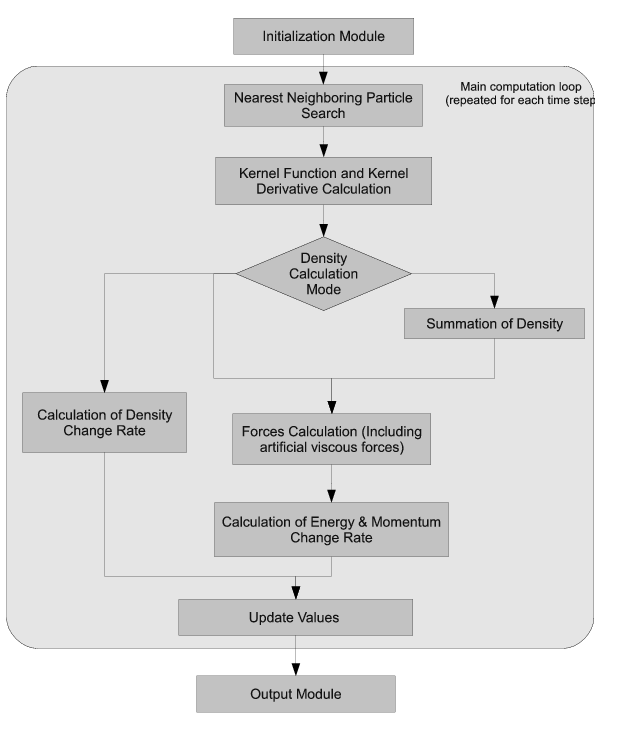
\includegraphics[width=1.0\textwidth]{Graphics/general_structure_SPH}
  \caption{Simulation domain for the cavity problem}
  \label{fig:PorositiesCavitiesSimuDomain}
\end{figure}



In a second step it is intended to send an acoustic wave over the cavity. This wave is generated by a temporally sinusoidal velocity perturbation on the left hand side domain edge. To match best the original experimental situation for optimum damping of the acoustic wave and for simulation purposes certain conditions have to be respected.
Starting with a fixed cavity diameter $d_\mathit{cavity,x}=0.3$ and a fixed domain size in x direction of $x_d=1$ the following values can be determined.
\begin{itemize}
 \item The distance $D$ from the cavity surface to the upper domain edge (symmetry line) is twice as big as the cavity diameter $d_\mathit{cavity,x}$: $D=2d_\mathit{cavity}00.6$
\item The depth $d_\mathit{cavity,y}$ of the cavity from surface to bottom is twice as big as the cavity diameter: $d_\mathit{cavity,y}=2d_\mathit{cavity,x}=0.6$. 
\item The frequency $f$ of the velocity perturbation for optimum damping obeys the condition $f=N\frac{U_\mathit{inf}}{2 D}$ with $N$ being a positive integer and $U_inf$ the steady state flow velocity at the upper domain edge.
\item In x direction the domain has to be wide enough for the acoustic wave to be fully generated at the LHS domain edge before the beginning of the wave reaches the RHS egde.
The condition for the domain width $x_d$ is therefore: $x_d=(U_\mathit{inf}+a)T$ where $a$ is the local sound speed at the upper domain edge and $T=\frac{1}{f}$ the periodical time of the acoustic wave. 
\item The sinusoidal velocity perturbation with an amplitude of 5\% of $U_\mathit{inf}$ has the form $ U_\mathit{pert}(t)=U_\mathit{pert,0}\sin(\omega t)$ with $U_\mathit{pert,0}=0.05 U_\mathit{inf}$ and $\omega=2\pi f$
 
\end{itemize}
Depending on the results of the steady state cavity flow, which are needed to obtain the values for $U_\mathit{inf}$ and $a$, the perturbation frequency $f$ is chosen in accordance with the condition on the domain size. The perturbation amplitude $U_\mathit{pert,0}$ can then be determined as well.

\paragraph {Initiation}

The particles are initialized with the following data (TABLE) and their distribution is generated on the basis of a rectangular grid for the whole rectangular domain by the program {\tt create\_ICCavity.cpp} in the {\tt scripts/InitCondPorosities} folder. It is only within the simulation program that the particles not needed for the simulation are discarded and the particles located within the solid walls are declared ghost particles. The necessary geometrical information for these operations is managed in the corresponding {\tt SolidObstacles} class called {\tt Cavity} of the simulation program.
However this information must be provided to the program by the particle initialization file (.ivs). Therefore, in the particle distribution generator {\tt create\_ICCavity.cpp} one has to specify the corresponding cavity data before the -ivs file is created. Detailed instructions on the initialization process with a schematic of the geometrical situation are contained in the {\tt README} file in {\tt InitCondPorosities}.
Note: the linear exprapolation approach for the ghost particle properties does only work for convex boundary curvatures. Besides it needs a clearly defined tangent for each point on the ghost particle surface. This is not the case in the cavity corners.
A more complex extrapolation approach conceived by \cite{Yildiz2009} would have to be implemented for this surface geometry. Therefore, the simple constant property approach is employed for the assignment of ghost particle values.
 



\subsubsection{Porosities -- flow through obstacles}
\label{sec:SimuSetup_flowThroughObstacles}

Generally introduced in section (\ref{sec:PorositiesCircularObstacles}), the configuration is modeled for the simulation by a domain with solid Cylinders at the domain corners and periodical boundary conditions at all sides as shown in figure (\ref{fig:PorositiesCircularObstacles_simuDomain}). 

\begin{figure}[!htbp]
  \centering
     %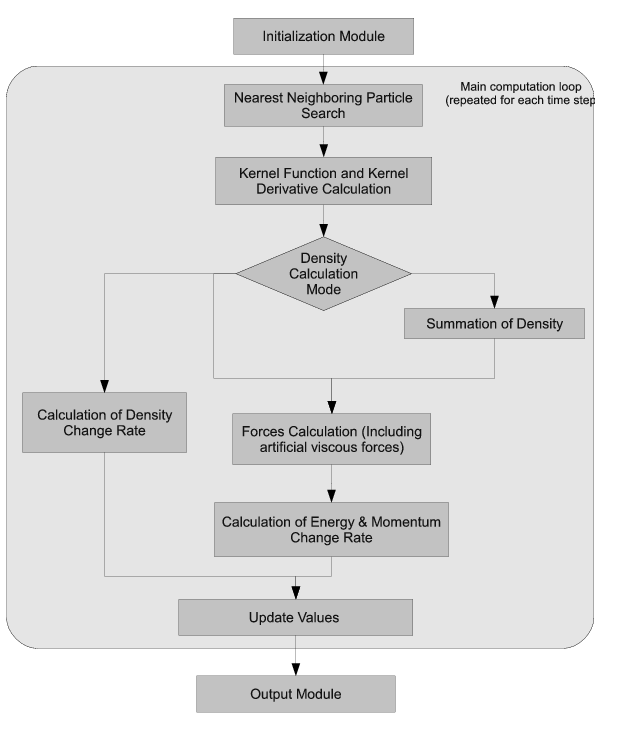
\includegraphics[width=1.0\textwidth]{Graphics/general_structure_SPH}
  \caption{Simulation domain for the cavity problem }
  \label{fig:PorositiesCavitiesSimuDomain}
\end{figure}

 The entire simulation setup is given in table TABLE and the particle properties of the real particles as created by the initialization files are summarized in the following table:
\linebreak[2]
TABLE
\linebreak[2]

Concerning the particle placement, three approaches are used, essentially inspired by Morris \cite{Morris1997, Zhu1999}. In any of the particle generator programs, one has to specify the location of the cylinders so their geometrical data can be communicated to the simulation program by the .ivs file. At the level of the .ivs file it makes no difference if a particle is a real particle or a ghost particle. For, in any case where {\tt solidObstacles} are involved, the declaration of a particle as ghost particle (and thus its immobilization) and also the removal of any ghost particles further than $l_s$ (if density evolved: $2l_s$) away from the obstacle surface is conducted within the simulation program. 

\begin{itemize}

 \item Uniform square lattice\\
  All particles are placed according to one continuous square lattice filling the entire calculation domain, no matter if there is a solid cylinder or not. This method
  models the cylinder surface very poorly for low resolutions.
(in this case mass initialization can be done within the program by interpolation)

\item Square lattice for real particles and circular layers for cylinders\\
This approach fills the cylinder areas with particles placed on concentric circles with the cylinder center as the corresponding cylinder origin.
Such a cylinder treatment was suggested by Morris \cite{Zhu1999} consists of a pseudo--hexagonal (ghost) particle arrangement within a solid cylinder of radius $R_cyl$. The domain of real particles is in a first case (not investigated by Morris) still filled with a rectangular lattice arrangement. To ensure that both the ghost particles and the cylinder particles placement result in the same density for equi-mass particles, the volume associated to a particle has to be the same for the rectangular case and the (pseudo) hexagonal case. Therefore if the particle spacing is $dx$ for the rectangular lattice, the corresponding spacing for the hexagonal case is determined by the relation $dx_\mathit{hex}^2=\frac{2}{\sqrt(3)}dx^2$. As the spacing in the cylinders is based on curved layers this is only an approximation and the value $dx_hex$, that is applied here, is selected in a way to obtain the best fit with the density in the real particles domain.

 The ghost particles are placed within the cylinder as follows:  .
  \begin{itemize}

   \item Supposing that the particle spacing on the circle representing the cylinder surface should be approximately $dx_\mathit{hex}$, the number of particles per circle or layer, which remains constant for all circles, is $N_{p,\mathit{layer}}={\mathit round}(2\pi R_\mathit{cyl}/dx)$. Here the particle distance is approximated by the arc--length between two particles.

\item Determine the angle increment in polar coordinates between two particles:
  $d\phi=2\pi/N_{p,\mathit{layer}}$. This is the same for all layers as the number of particles per layer remains constant. 
 \item Starting at a certain $\phi_0$ all particles on the first layer, which has the radius of the cylinder, are placed every $d\phi$. The actual particle positions in Cartesian coordinates are obtained by $x=r \cos(\phi)$ and $y=r \sin(\phi)$.

\item If one layer of particles is completely filled, the next circle with a new radius $R_\mathit{new}=R_\mathit{old}-\sqrt{3}dx/2$ is placed the same way as the one before. Only the starting angle for the first particle is now shifted, so a pseudo hexagonal particle placement is obtained: $\phi_{0,\mathit{new}}=\phi_{0,\mathit{old}}+d\phi/2$. This way particles on every second circle are placed at the same angle.

\item Once a distance of at least $l_s$ (if density evolved $2l_s$) away from the cylinder surface is covered, the particle placement may be stopped.
  \end{itemize}
The real particle area between the domain is filled with particles according to a regular lattice. 
The sensible point of this particle initialization is the interface between the regular lattice and the circular arrangement at the cylinder surface.
As the mass of all particles is desired to be the same, a mass initialization within the simulation program by smoothing, which would lead to mass variations of particles around the interface, is not possible. Therefore mass is initialized externally by the initialization file ({\tt .ivs}) to the same value for all particles. This is why errors in density because of the irregular transition of the particle lattices may occur around the cylinder surfaces.
One adjustment parameter is the margin in distance between the cylinder surface, which at the same time is the position of the last layer of ghost particles, and the closest real particle to this cylinder surface. A value of $\sqrt{3}dx/2$  seems to be reasonable for this margin.


\item hexagonal lattice for real particles and circular layers for cylinders
The placement of particles in the cylinder area does not differ from the above case. Instead of a rectangular lattice however, the real particles are now arranged according to a hexagonal pattern  as shown in figure (\ref{fig:HexagonalLattice}). A hexagonal lattice is more dense than a standard rectangular lattice with same minimum particle distance $dx$. This way the area around the cylinders, where there is a transition between two lattice types, can be filled in a smoother manner than with the above rectangular lattice. Furthermore, the hexagonal character the general advantage that 
it makes the particle distribution more isotropic on the micro--scale.

\begin{figure}[!htbp]
  \centering
     %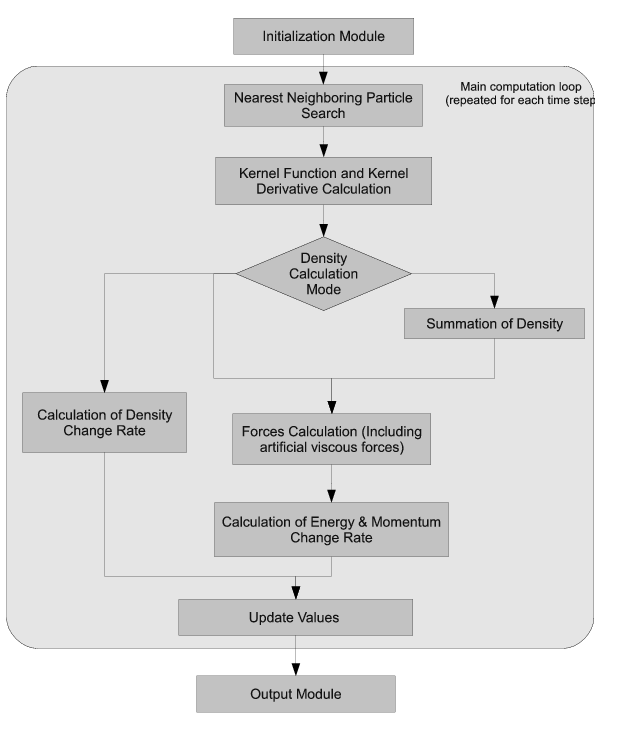
\includegraphics[width=1.0\textwidth]{Graphics/general_structure_SPH}
  \caption{Hexagonal lattice for real particle placement}
  \label{fig:HexagonalLattice}
\end{figure}

As the particle spacing is $\Delta$ (the closest particle distance) in one direction and $\Delta'=\sqrt{3}\Delta/2$ in the other, there will be in general an irregularity in particle spacing at one of the domain edges for a squared calculation domain with size $l_d$. To fill the domain with particles in a regular manner nonetheless, the particle spacing in the second direction is not chosen exactly $\sqrt{3}\Delta/2$ but the closest value which respects the condition $N \Delta'=l_d$, where $N$ is a positive integer. For a domain size of $l_d=1$ and a closest particle spacing of $dx=0.02$ as for the above cases, the chosen spacing in the second direction is $\Delta'=1/58\approx0.01724$ while the exact value to obtain a perfectly hexagonal lattice would be $\Delta'\approx0.01732$. 
Again the particle's mass is initialized externally due to the irregularities around the cylinder surfaces. The value for the mass is determined by the desired density and the volume associated to one particle. For the given geometrical situation this volume is $V=\frac{1}{50\cdot58}\approx3.448\cdot10^{-4}$.

\end{itemize}



\chapter{Results}
\label{sec:Results}
This chapter presents the results obtained with the developed codes. The focus clearly lies on the 2D code which is finally used to simulate the porosity configuration. However, as the 1D code has be introduced in the chapter before, an example of its application to the 1D shock-tube--problem is shown in the following section. It serves for a first qualitative discussion of the shock--tube results that can be obtained with SPH.
The 2D code result section mainly features the results of the previously introduced test--cases (\ref{sec:GenIntroTestCases}) and finally a simulation of the flow in a porosity.

As it is not practical to label every result with all the settings used in the simulation generating it, these settings are summarized for each test--case in the corresponding paragraph of section (\ref{sec:simuSetupTestCases}).

\section{1D SPH code}
\label{sec:1DSPHcodeResults}
As mentioned above, the 1D SPH--code, which only serves demonstration purposes and does not have any practical use, incorporates the simulation setup for the shock-tube--problem. The code is developed to get familiarized with the SPH implementation and to provide a very simple playground to experiment and find the right set of SPH equations for compressible flows. Figure (\ref{fig:1DSPHresults}) shows the results of a simulation with a constant smoothing length of $h=0.0065$ and a constant mass particle distribution, i.\ e.\ with different particle spacings on the LHS and RHS of the shock--tube problem (see paragraph (\ref{sec:1DSPHcode_functions_setupSim})) for an introduction of the two shock--tube--specific particle distributions, namely with constant mass or constant spacing. The complete simulation settings for this example can be found in section (\ref{sec:simuSetup1DSPHcode}). 

\begin{figure}[!htbp]

\centering
\label{fig:1DSPHresults}
\subfigure[]{
\label{fig:1DSPHreultsVelocity}
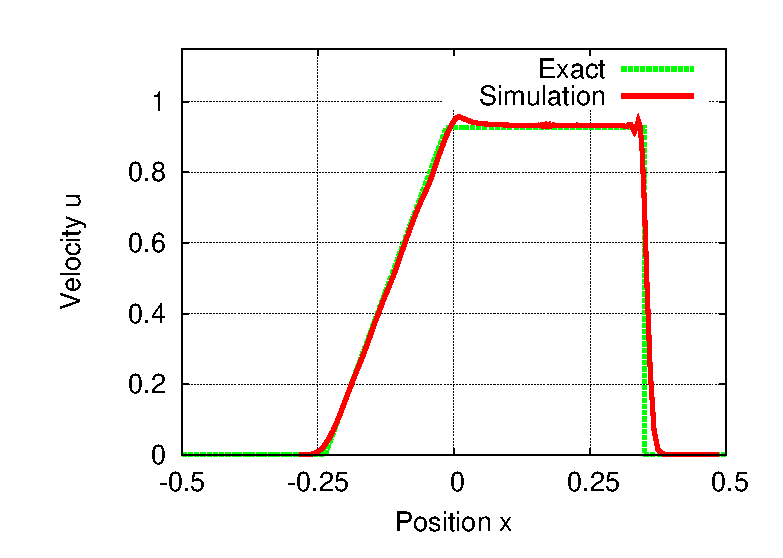
\includegraphics[width=7cm]{Graphics/results/1DCode/velocity}}
\subfigure[]{
\label{fig:1DSPHreultsDensity}
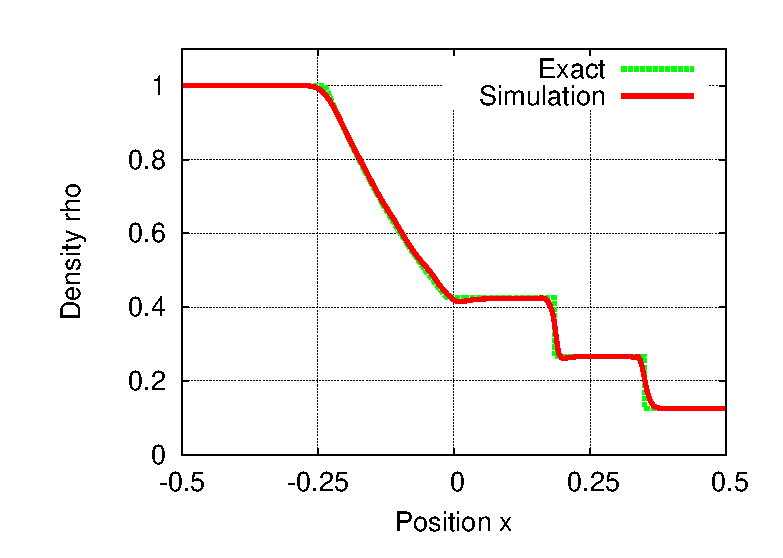
\includegraphics[width=7cm]{Graphics/results/1DCode/density}}
\subfigure[]{
\label{fig:1DSPHreultsPressure}
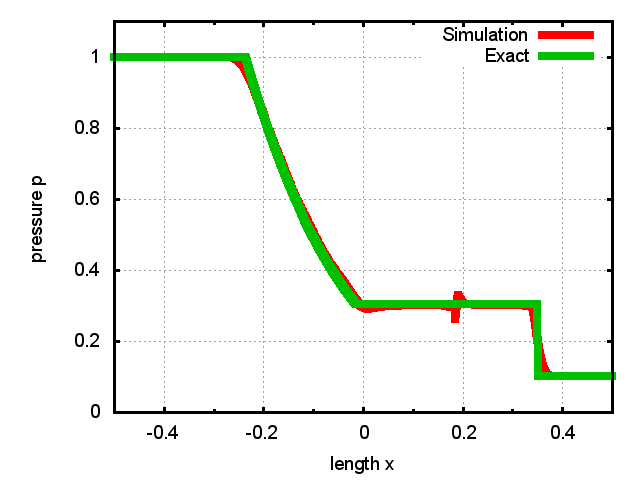
\includegraphics[width=7cm]{Graphics/results/1DCode/pressure}}
\subfigure[]{
\label{fig:1DSPHreultsEnergy}
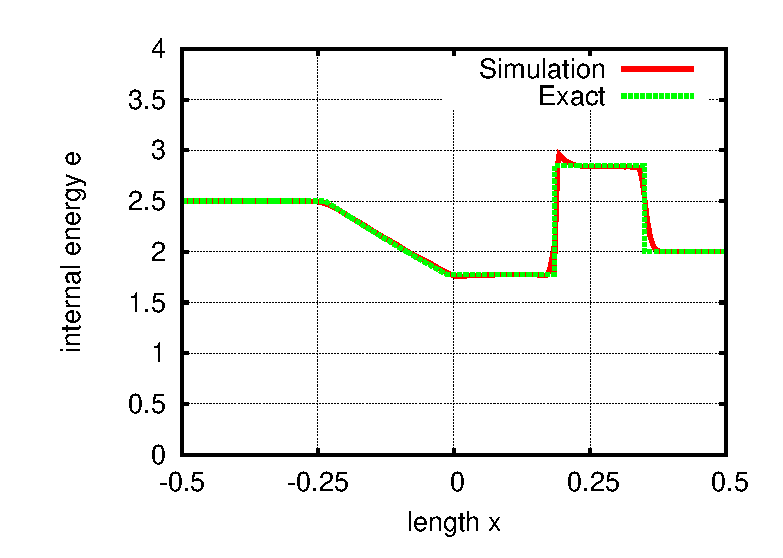
\includegraphics[width=7cm]{Graphics/results/1DCode/energy}}

\caption[Example of a shock-tube result obtained with the 1D SPH--code]{Example of a shock-tube result obtained with the 1D SPH--code for a simulation time of $t=0.2$ contrasted with the exact analytical solution (see section (\ref{sec:TestCases_1DshockTube})): \subref{fig:1DSPHreultsVelocity} velocity profile; \subref{fig:1DSPHreultsDensity} density profile; \subref{fig:1DSPHreultsPressure} pressure profile; \subref{fig:1DSPHreultsEnergy} profile of the internal energy.}

\end{figure}

While quantitative evaluation of the shock--tube results will only be done with the 2D code, some qualitative statements can already be made at this place.
Comparison with SPH--solutions from literature shows that the profiles presented in figure (\ref{fig:1DSPHresults}) are typical. Taking for example the results of \cite{Liu2003} or \cite{Monaghan1985} one can observe the same tendencies: the shock front is resolved within several (2-3) smoothing lengths. The same applies for the contact discontinuity in the variables where there are discontinuities ($\rho, e$). Furthermore the fact that the internal energy is overestimated at the high energy side of the contact discontinuity seems to be typical as well and a remedy is found by smoothing the initial energy profile before starting the actual calculation \cite{Monaghan2005,Price2004}. On the other hand by smoothing initial conditions, one looses accuracy in the resolution of the rarefaction \cite{Price2004}.  The oscillations after the shock front (notably in the velocity profile) are normal as well and by the way are one of the reasons why an artificial viscosity has to be used for shock simulations: besides preventing particles from interpenetrating at the shock front, another main function of the artificial viscosity is to dissipate these velocity oscillations \cite{Monaghan2005,Sigalotti2006}.
Finally, the little blip in the pressure profile at the contact discontinuity is known in literature as well. It can be removed by introducing a small amount of heat diffusion into the energy equation \cite{Monaghan1992}. The logic behind the use/effect of this artificial heat diffusion term is the following: the artificial viscosity, which is also taken into account in the energy equation (see section (\ref{sec:ArtVisc})), may produce excessive heating \cite{Sigalotti2006}. This phenomenon is commonly referred to as wall--heating errors (originally discovered by \cite{Noh1978}), and it can be significantly reduced by introducing an artificial heat diffusion term to the internal energy equation. The exact form of this term however, differs from author to author. Monaghan \cite{Monaghan1992} for example only suggests a constant value of heat diffusion to be added for the shock--tube case. More sophisticated, variable heat diffusion terms are proposed by Price \cite{Price2004} and Sigalotti \cite{Sigalotti2006}.
However, as the wall--heating error only occurs for strong shocks and as there are no shocks at all expected in the application of this code, which is a high enthalpy flow through porous media, this ``trick'' is not implemented. 

The first qualitative evaluation of the simulation results implies that the equations used for the compressible 1D SPH code are the good ones and encourages the integration of these equations in the more complex 2D SPH code, where extensive quantitative evaluation is performed.  

%see danial Price2004 Thesis for effect of smoothing: He smoothes rho,p and does not get the energy peak at the discontinuity for the smoothed initial conditions. (I smooth density as well, (and I think pressure is therefore smoothed as well (as recalculated from smoothed density before used anywhere in the program (BUT I HAVE TO CHECK THAT IN THE PROGRAM BEFOR WRITING THE FINAL VERSION))
%I also have to check HOW the variables are smoothed (I smooth rho just by applying the summation formula but Sigalotti2006 uses a different smoothing formula...)
 
%More exact results (falsch, peaks gehn zwar weg, aber dafür rarefaction nur verschmiert aufgelöst!!!) for the shock-tube problem can be obtained by smoothing all initially discontinuous quantities ($\rho, u, e$) at the beginnig of the calculation. This was originally proposed by \cite{Monaghan1997}. Applying a variable smoothing length also improves the results\cite{Monaghan2005}. 

%...Monaghan05 p.1739... not shock width important but pre and after shock values...

\section{2D SPH code}
\label{sec:2DSPHcodeResults}

The 2D SPH code underwent extensive testing at the various stages of development. After modification towards compressible flow capabilities, the shock--tube test case was investigated and propagation of acoustic waves was analyzed. In a subsequent step viscosity implementation has been tested by the Taylor--Green flow and independently of any flow problem the implemented heat conduction model was verified by a pure conduction test--problem. The compressible Couette flow in which different phenomena are combined concludes the testing of the flow models. For the porosity simulation a different boundary condition approach than the one used for the domain edges is implemented. Therefore this method has to be tested separately, which is done by means of a Poiseuille--flow before finally the actual porosity configurations are exemplarily simulated.

\subsection{Shock--tube test case}
\label{sec:2DSPHcodeResults_Shock}
The shock--tube case is used to conduct several series of simulations aimed at the verification of the modified code and at assessing its convergence behavior %(IST DAS NICHT ABHÄNGIG VOM TESTFALL??) 
as well as the robustness versus perturbations in particle positions. 
First, the automatic time step control is exemplarily tested. Then the influence of the two approximation parameters $h$ and $dx$ on the simulation results is shown by means of a resolution study, which consists of two parts. One part where the smoothing length $h$ is varied at constant $dx$ and another part, where the resolution is increased at a constant ratio of $h/dx$. Ultimately, the perturbation study consists of a set of simulations with increasingly perturbed initial particle positions.

All the above tests are conducted for the four cases:
\begin{itemize}
 \item 1D particle distribution with constant spacing
  \item 2D particle distribution with constant spacing
 \item 1D particle distribution with constant mass
  \item 2D particle distribution with constant mass
\end{itemize}

Unless otherwise stated the simulation time for each shock--tube simulation is $t=0.2$. Other simulation settings as well as the entire set of initial conditions can be found in section (\ref{sec:2Dshock_simuSetup&Co}).

The nature of an exemplary shock--tube simulation result including explanations is already given in section (\ref{sec:1DSPHcodeResults}). It is still the same for the 2D code and therefore is not repeated at this place. Instead focus lies clearly on the evaluation of the error norms and profiles are shown only where they exhibit a particularity. However, the complete set of figures for each simulation run constituting the following analyzes can be found in the corresponding {\tt results} folder of {\tt sph-blitz}. The path to the respective folder is given for each of the following sets of simulation.

\subsubsection{Verification of time step criteria}

In section (\ref{sec:TmeStepChoice}) the criteria for a stable time step choice have been presented. In order to be sure that for the further studies of results, all errors are due to spatial discretization, the applied time stepping criteria are tested for correctness. As the shock--simulation includes artificial, but no real viscosity and no thermal conduction, the criteria in question are equations (\ref{eq:dtForce}) and (\ref{eq:dtCourantVisc}). Figure (\ref{fig:2DSPHresults_1D_CStimeVerif}) shows the evolution of the L-errors (see section (\ref{sec:employedNormDefinition})) for $\rho, u, e$ with varying time step evaluated in the whole domain and in areas 2 and 3 only (see section (\ref{sec:2Dshock_simuSetup&Co}). 
The errors taking into account the whole domain are generally higher than the ones that only focus on the after-rarefaction (area 3) and after-shock (area 2) values. The $L_{\infty}$ error which is not an integral error measure but the maximum value of each particle-wise error is naturally the biggest one, followed by the $L_2$ and then the $L_1$ errors. For the shock--tube case the global $L_{\infty}$ error is entirely determined by the shock--front, where the errors are locally biggest due to the finite shock resolution. Evaluated only for areas 2 or 3 the $L_{\infty}$ error captures often either oscillation maxima or the hangover of the non-exact shock or rarefaction resolution (rarefaction resolution non exact due to initial smoothing of density field) which reaches into the corresponding area.

The considerable increase of the error-values in area 2, particularly in the velocity field, starting at a time step size of around $dt\geq0.0025$ shows that temporal instability is indicated first in the after-shock area. A look at the plotted velocity-profile in figure (\ref{fig:2DSPHresults_dt_variat_oscillationU}) of one of these simulations confirms this, by showing severe oscillations directly after the shock area. It will turn out that the inaccuracy observed in the rarefaction in the same figure is particular to the constant spacing particle initiation, at least in 1D, and has nothing to do with temporal resolution.

\begin{figure}[!htbp]

\centering
\label{fig:2DSPHresults_dt_variat_oscillationU}
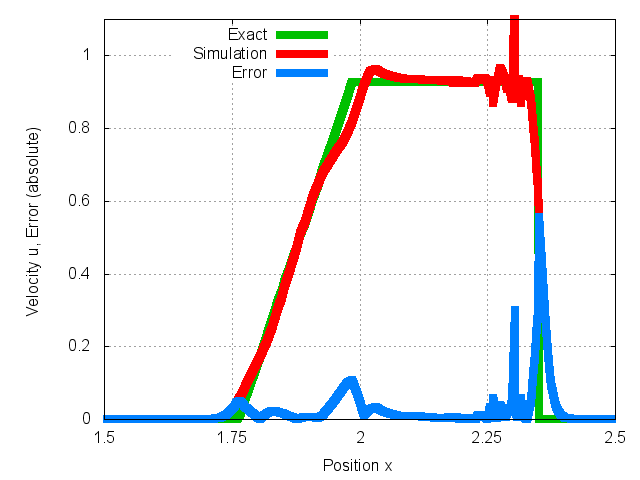
\includegraphics[width=7cm]{Graphics/results/ShockTube/1D_CS_LF_SD/dtVariat_dx005_SupLen03_dt03_Oscillations/Err_u00200000}
\caption[Velocity oscillations due to temporal instability]{Velocity profile after $t=0.2$ for a time step of $dt=0.002985$, which shows severe oscillations in the after--shock area due to a too big time step $dt$. The support length of the simulation is $0.03$ with an 1D particle distribution of constant spacing of $dx=0.005$.}

\end{figure}

Concerning the temporal resolution test again, values of $dt<0.0025$ can be considered as stable for this configuration and a look at the automatically determined time step ($dt=0.00198083$) shows it is just below this critical value, including a decent safety margin.

The residual errors in figure (\ref{fig:2DSPHresults_1D_CStimeVerif}) for $dt<0.0025$ can therefore be attributed to the spatial discretization error due to $dx$ (or better $h/dx$) and integral approximation error due to $h$. All results leading to figure (\ref{fig:2DSPHresults_1D_CStimeVerif}) can be found in {\tt sph-blitz/results/ShockTubeTestCase/1DpartDist\_constSpace\_LeapFrog/dtVariat\_dx005\_SupLen03}.

Another verification has also been conducted for a 2D constant spacing particle resolution. The time stepping criteria worked fine for this case as well. 




\begin{figure}[H]
\centering
\label{fig:2DSPHresults_1D_CStimeVerif}

\subfigure[tight][whole domain]{
\label{fig:2DSPHresults_1D_CStimeVerif_wholeRho}
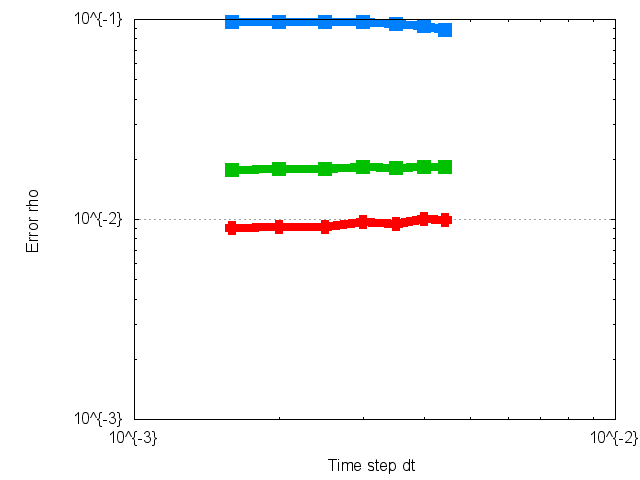
\includegraphics[width=5cm]{Graphics/results/ShockTube/1D_CS_LF_SD/dtVariat_dx005_SupLen03/WholeDomainRho}}
\subfigure[tight][area 3]{
\label{fig:2DSPHresults_1D_CStimeVerif_3Rho}
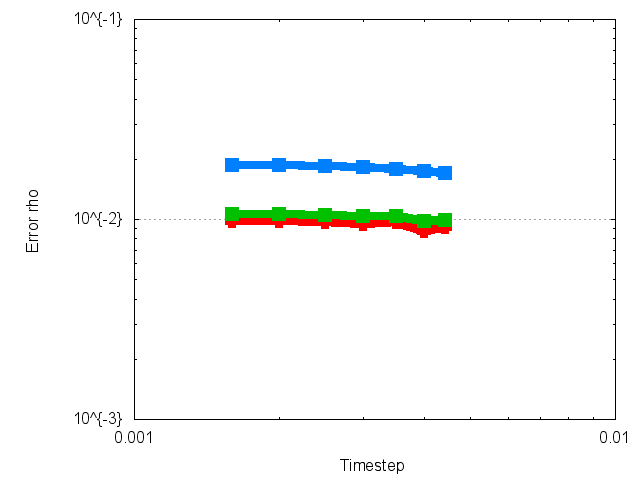
\includegraphics[width=5cm]{Graphics/results/ShockTube/1D_CS_LF_SD/dtVariat_dx005_SupLen03/Area3Rho}}
\subfigure[tight][area 2]{
\label{fig:2DSPHresults_1D_CStimeVerif_2Rho}
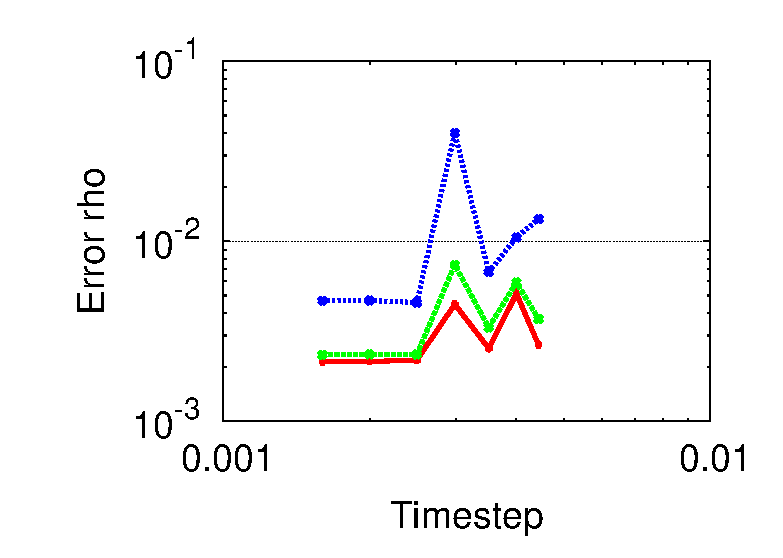
\includegraphics[width=5cm]{Graphics/results/ShockTube/1D_CS_LF_SD/dtVariat_dx005_SupLen03/Area2Rho}}
\subfigure[tight][whole domain]{
\label{fig:2DSPHresults_1D_CStimeVerif_wholeU}
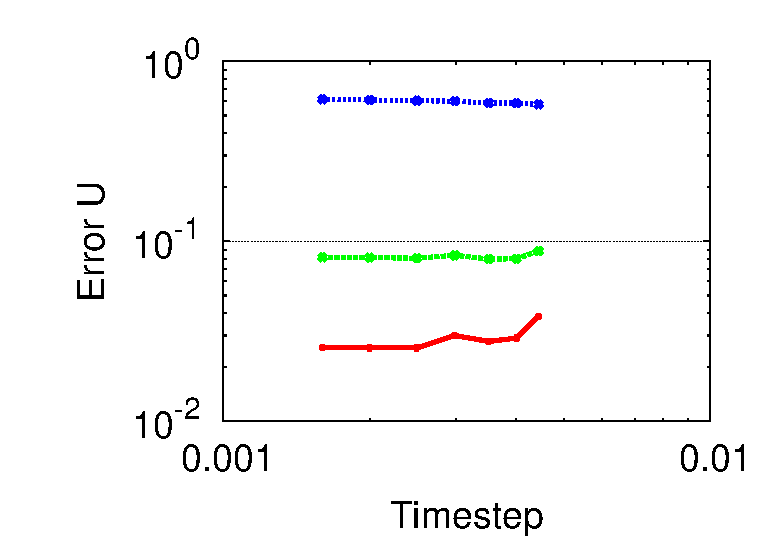
\includegraphics[width=5cm]{Graphics/results/ShockTube/1D_CS_LF_SD/dtVariat_dx005_SupLen03/WholeDomainU}}
\subfigure[tight][area 3]{
\label{fig:2DSPHresults_1D_CStimeVerif_3U}
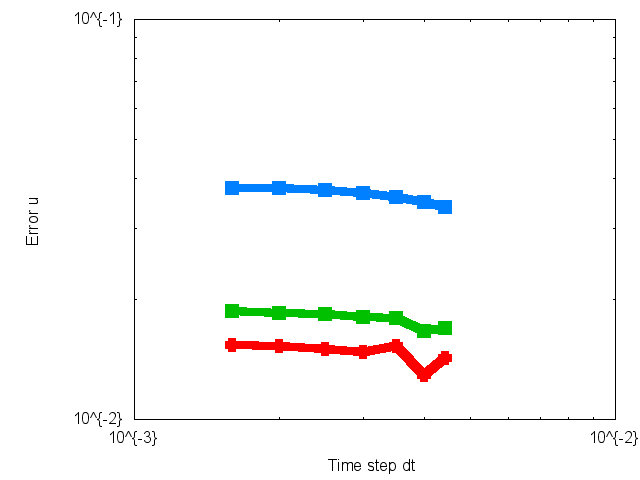
\includegraphics[width=5cm]{Graphics/results/ShockTube/1D_CS_LF_SD/dtVariat_dx005_SupLen03/Area3U}}
\subfigure[tight][area 2]{
\label{fig:2DSPHresults_1D_CStimeVerif_2U}
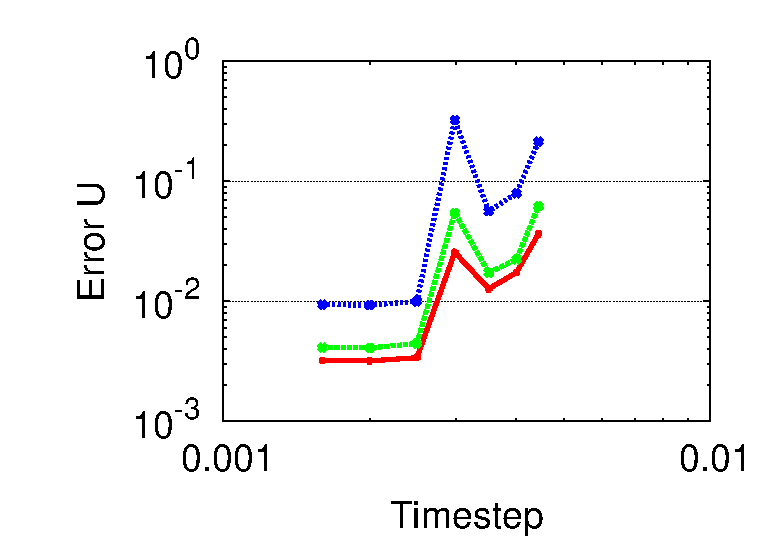
\includegraphics[width=5cm]{Graphics/results/ShockTube/1D_CS_LF_SD/dtVariat_dx005_SupLen03/Area2U}}
\subfigure[tight][whole domain]{
\label{fig:2DSPHresults_1D_CStimeVerif_wholeE}
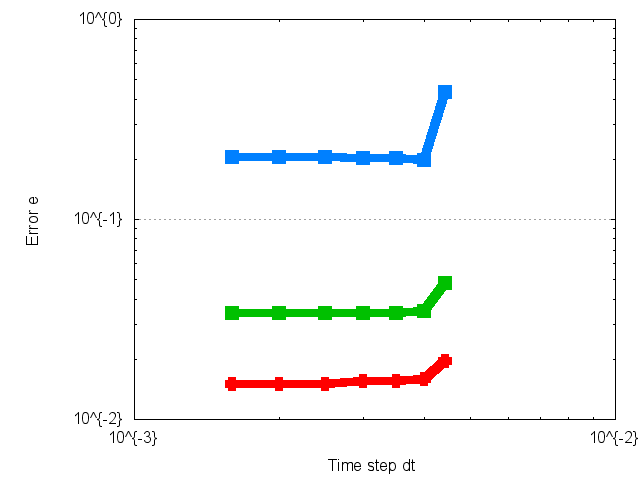
\includegraphics[width=5cm]{Graphics/results/ShockTube/1D_CS_LF_SD/dtVariat_dx005_SupLen03/WholeDomainE}}
\subfigure[tight][area 3]{
\label{fig:2DSPHresults_1D_CStimeVerif_3E}
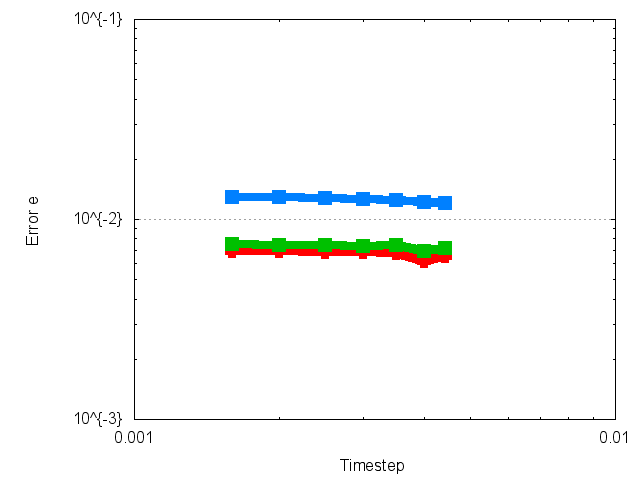
\includegraphics[width=5cm]{Graphics/results/ShockTube/1D_CS_LF_SD/dtVariat_dx005_SupLen03/Area3E}}
\subfigure[tight][area 2]{
\label{fig:2DSPHresults_1D_CStimeVerif_2E}
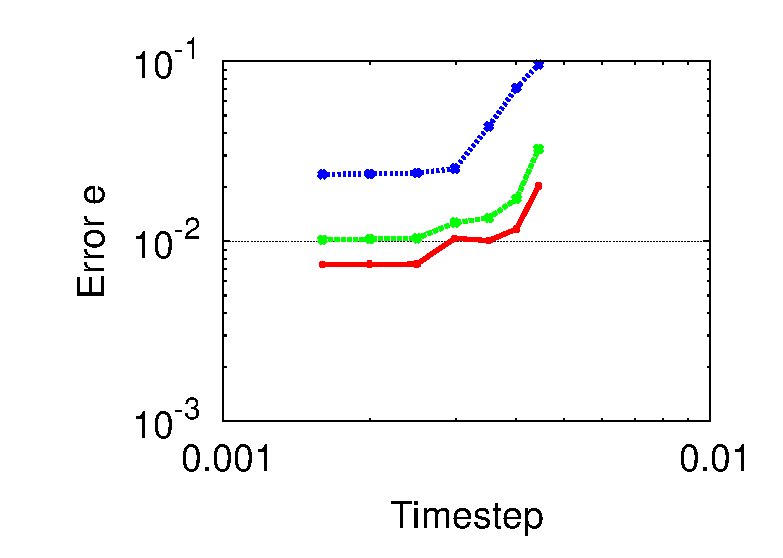
\includegraphics[width=5cm]{Graphics/results/ShockTube/1D_CS_LF_SD/dtVariat_dx005_SupLen03/Area2E}}

\caption[Convergence Shock-tube 1D constant spacing particle distribution]{L--norm errors of $\rho, u, e$ for a series of simulation with a varying time step $dt$. The support length is $0.03$ with an 1D particle distribution of constant spacing of $dx=0.005$.}

\end{figure}

\begin{figure}[H]
\centering
\label{fig:2DSPHresults_tempRes_vProfile}

\subfigure[tight][whole domain]{
\label{fig:2DSPHresults_1D_CS_dx_const_wholeRho}
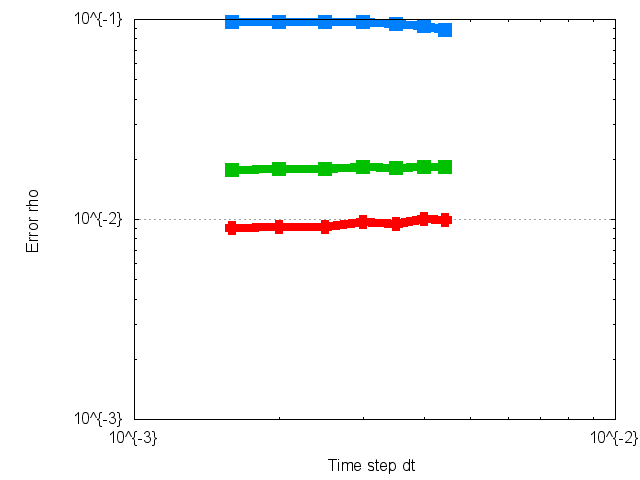
\includegraphics[width=5cm]{Graphics/results/ShockTube/1D_CS_LF_SD/dtVariat_dx005_SupLen03/WholeDomainRho}}
\end{figure}



\subsubsection{Resolution Study - spacing held constant}
\label{sec:2DSPH_results_shock_resSTudy_dx=const}
The purpose of this set of simulations is to evaluate the influence of a smoothing length variation with a constant particle distance. There is expected to be an optimum value for $h$ in this case: For small $h$, the ratio $h/dx$ and therefore the number of neighboring particles in the support domain of a certain particle will be to small to ensure a correct discrete representation of the integral interpolant. On the other hand, greater smoothing lengths mean a worse resolution of local phenomena and here especially shocks, which will increase the error considerably. 


\paragraph{1D constant spacing particle distribution}

Having a look at figure (\ref{fig:2DSPHresults_1D_CS_dx_const}), one sees the above anticipated tendency. Especially the integral errors ($L_1,L_2$) calculated for the whole domain show a clear minimum at a support length of around 0.025, which means that the number of neighboring particles is 8. 
The increase of the errors for medium support lengths in area 3 is due to a drift of the inaccuracy in the rarefaction wave into area 3. Otherwise this inaccuracy, which is always present for this set of simulations, is not taken into account for area 3 but only in the global error calculation. 
If the support length becomes too big, not only the shock resolution gets poorer, but also the after--shock velocity profile becomes bumpy.

\begin{figure}[H]
\centering
\label{fig:2DSPHresults_1D_CS_dx_const}

\subfigure[tight][whole domain]{
\label{fig:2DSPHresults_1D_CS_dx_const_wholeRho}
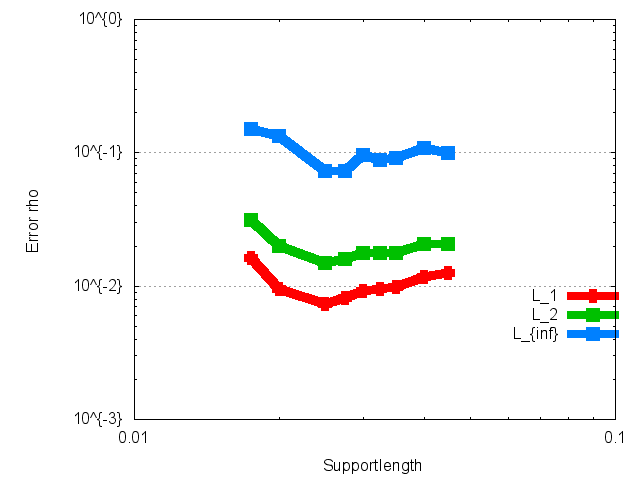
\includegraphics[width=5cm]{Graphics/results/ShockTube/1D_CS_LF_SD/SuppLenVariat_dx005_dt0025/WholeDomainRho}}
\subfigure[tight][whole domain]{
\label{fig:2DSPHresults_1D_CS_dx_const_3Rho}
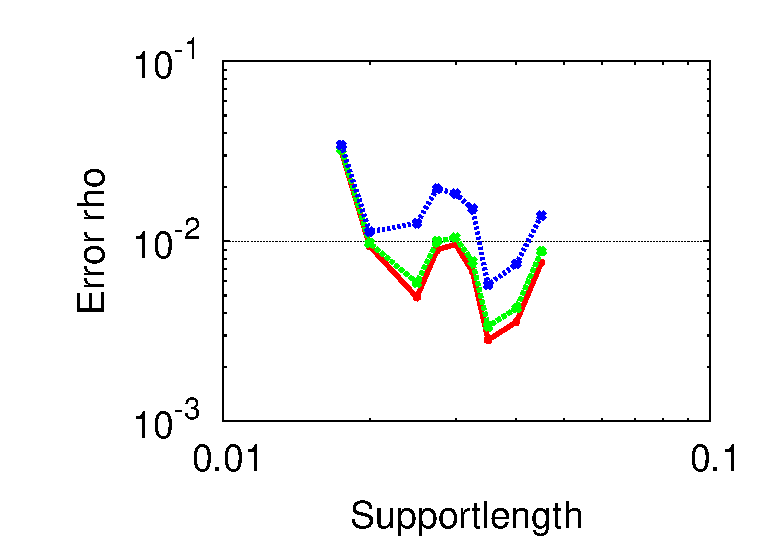
\includegraphics[width=5cm]{Graphics/results/ShockTube/1D_CS_LF_SD/SuppLenVariat_dx005_dt0025/Area3Rho}}
\subfigure[tight][whole domain]{
\label{fig:2DSPHresults_1D_CS_dx_const_2Rho}
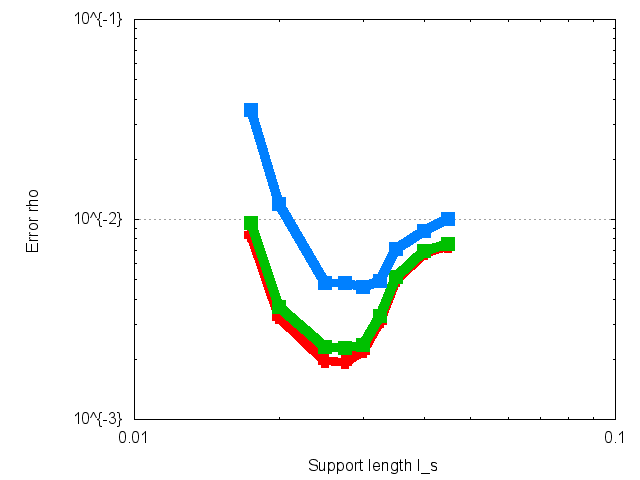
\includegraphics[width=5cm]{Graphics/results/ShockTube/1D_CS_LF_SD/SuppLenVariat_dx005_dt0025/Area2Rho}}
\subfigure[tight][area 3]{
\label{fig:2DSPHresults_1D_CS_dx_const_wholeU}
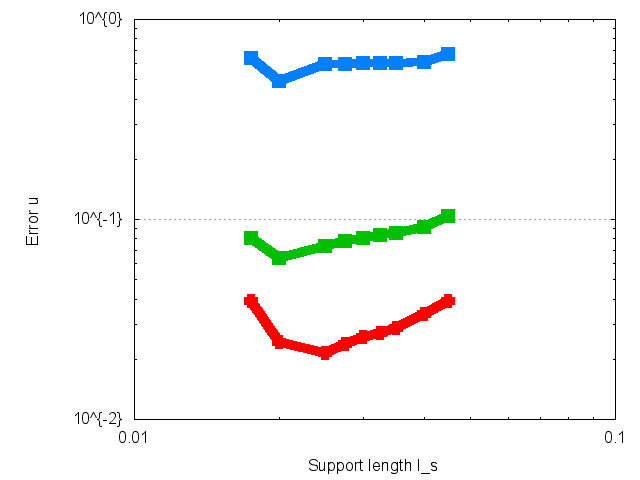
\includegraphics[width=5cm]{Graphics/results/ShockTube/1D_CS_LF_SD/SuppLenVariat_dx005_dt0025/WholeDomainU}}
\subfigure[tight][area 3]{
\label{fig:2DSPHresults_1D_CS_dx_const_3U}
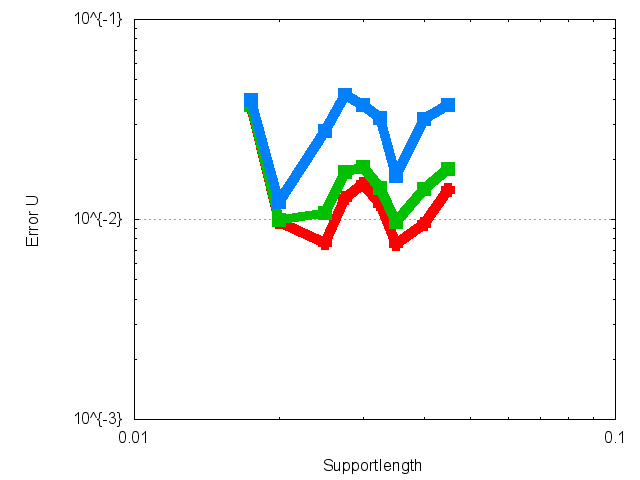
\includegraphics[width=5cm]{Graphics/results/ShockTube/1D_CS_LF_SD/SuppLenVariat_dx005_dt0025/Area3U}}
\subfigure[tight][area 3]{
\label{fig:2DSPHresults_1D_CS_dx_const_2U}
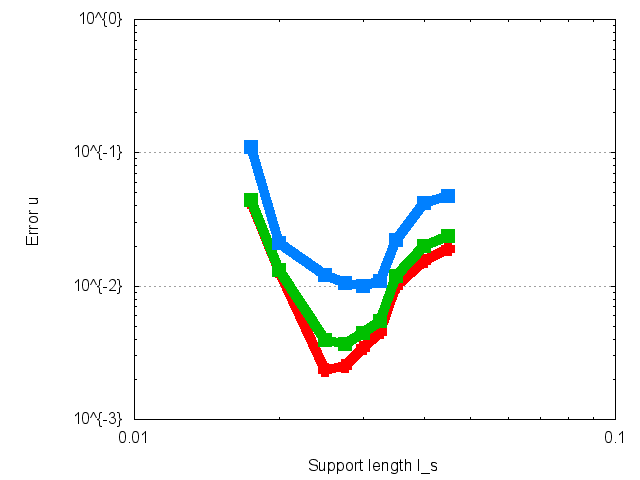
\includegraphics[width=5cm]{Graphics/results/ShockTube/1D_CS_LF_SD/SuppLenVariat_dx005_dt0025/Area2U}}
\subfigure[tight][area 2]{
\label{fig:2DSPHresults_1D_CS_dx_const_wholeE}
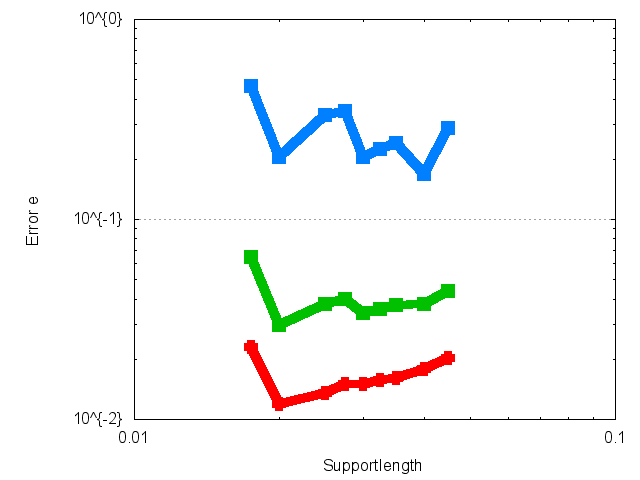
\includegraphics[width=5cm]{Graphics/results/ShockTube/1D_CS_LF_SD/SuppLenVariat_dx005_dt0025/WholeDomainE}}
\subfigure[tight][area 2]{
\label{fig:2DSPHresults_1D_CS_dx_const_3E}
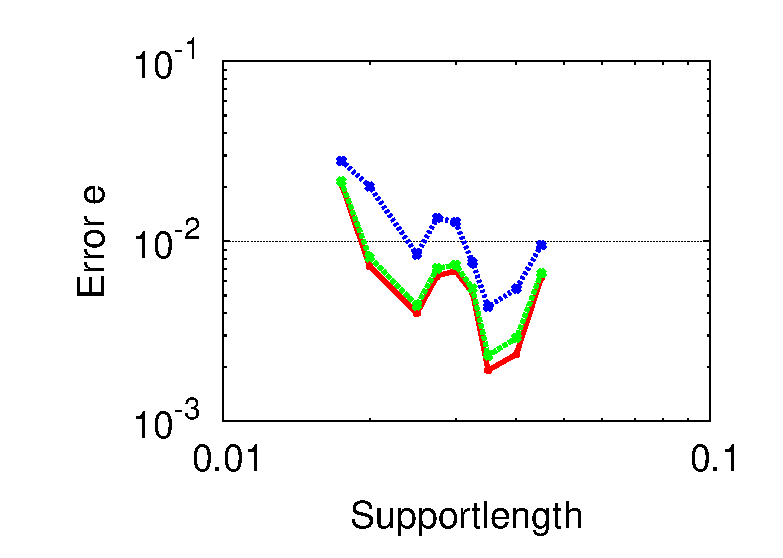
\includegraphics[width=5cm]{Graphics/results/ShockTube/1D_CS_LF_SD/SuppLenVariat_dx005_dt0025/Area3E}}
\subfigure[tight][area 2]{
\label{fig:2DSPHresults_1D_CS_dx_const_2E}
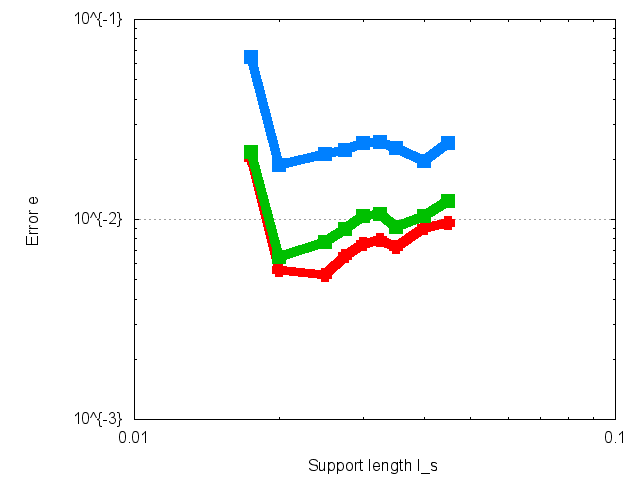
\includegraphics[width=5cm]{Graphics/results/ShockTube/1D_CS_LF_SD/SuppLenVariat_dx005_dt0025/Area2E}}

\caption[Convergence Shock-tube 1D constant spacing particle distribution]{L--norm errors of $\rho, u, e$ for a series of simulation with a varying support length and a constant particle spacing of $dx=0.0025$.}

\end{figure}



\paragraph{2D constant spacing particle distribution}

The same procedure as in the paragraph just above is now conducted with a 2D particle distribution of a spacing of $dx=dy=0.005$ and again the optimum support length is found to be around 0.025, like for the corresponding 1D particle distribution. Otherwise the results look the same as in figure (\ref{fig:2DSPHresults_1D_CS_dx_const}) and are therefore only presented in the Appendix.

When having a look at the evolution of the particle positions during a simulation, which is displayed in figure (\ref{fig:2DSPHresults_CS_drifting}) it is remarkable that the particles at the contact discontinuity drift away from their originally perfectly lined up position. However this behavior seems stable for support lengths $\geq0.02$ (at least within the simulation time of 0.2)(figure (\ref{fig:2DSPHresults_CS_drifting_suplen02}) and is visually not detectable anymore for a support length of $\geq0.35$. In the simulation with a support length of 0.015 particles around the contact discontinuity are completely drifting  away from their original position, forming a bizarre structure - it seems as if they were attracted by the symmetrically drifting particles of the next row (figure (\ref{fig:2DSPHresults_CS_drifting_suplen015}). 
The drifting is probably an expression of what Monaghan \cite{Monaghan2005} (shocks in 2D/3D can be noise - at least with current algorithms) and Rasio \& Shapiro \cite{Rasio1991} (in $>$1D there is a much bigger effect of numerical noise for shock tube simulation) state in their papers.

\begin{figure}[!htbp]
\centering
\label{fig:2DSPHresults_CS_drifting}
\subfigure[support length 0.015]{
\label{fig:2DSPHresults_CS_drifting_suplen015}
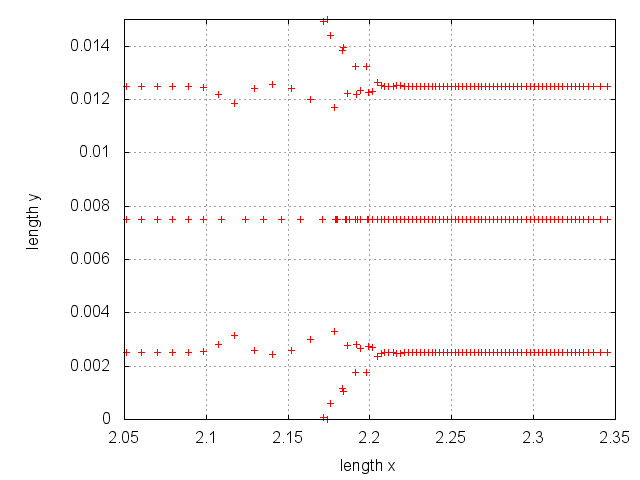
\includegraphics[width=7cm]{Graphics/results/ShockTube/q1D_CS_LF_SD/supLenVariat_dxdy005/Drifting/suplen015/x_y_plane00200653}}
\subfigure[support length 0.02]{
\label{fig:2DSPHresults_CS_drifting_suplen02}
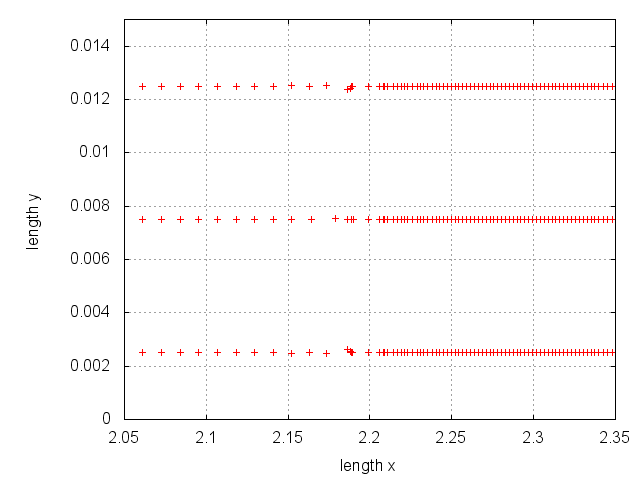
\includegraphics[width=7cm]{Graphics/results/ShockTube/q1D_CS_LF_SD/supLenVariat_dxdy005/Drifting/suplen02/x_y_plane00200841}}

\caption[Particle drifting for 2D distribution]{particle drifting originating at the contact discontinuity for different support lengths.}

\end{figure}

It is/are not only the particle positions that loose their perfect uniformity in the y- direction, but also the particle properties. This scattering is quantified by a variance calculation which shows results unequal zero in the contact discontinuity area.
Figure (\ref{fig:2DSPHresults_CS_variance}) shows exemplarily the variances of $\rho$ and $v$ along the shock--tube with significant amplitudes in the above mentioned area.

\begin{figure}[!htbp]
\centering
\label{fig:2DSPHresults_CS_variance}
\subfigure[support length 0.015]{
\label{fig:2DSPHresults_CS_variance_suplen015}
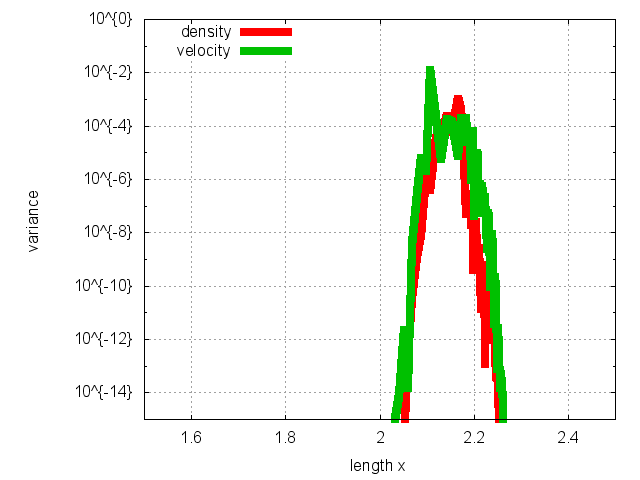
\includegraphics[width=7cm]{Graphics/results/ShockTube/q1D_CS_LF_SD/supLenVariat_dxdy005/Variance/suplen015/VarianceSupLen015}}
\subfigure[support length 0.02]{
\label{fig:2DSPHresults_CS_variance_suplen02}
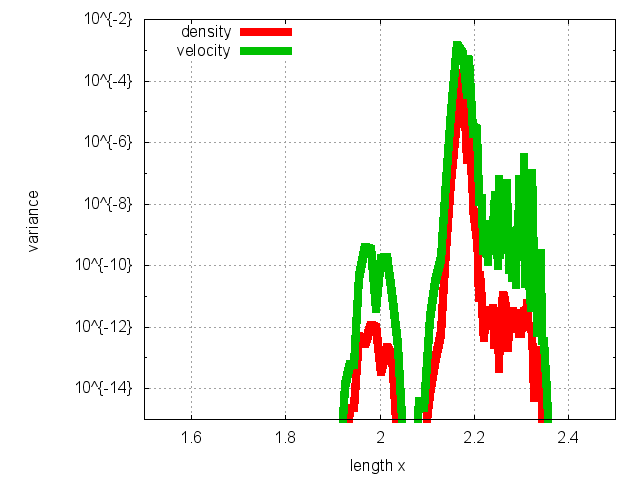
\includegraphics[width=7cm]{Graphics/results/ShockTube/q1D_CS_LF_SD/supLenVariat_dxdy005/Variance/suplen02/VarianceSupLen02}}

\caption[]{Variance evolution along the shock--tube for the averaging of velocity and density at different support lengths.}

\end{figure}

The trend, that has been observed for the drifting, namely a decreasing effect with greater support length can roughly also be observed for the scattering of the x-position as well as all particle properties (figure (\ref{fig:2DSPHresults_CS_varianceVersusSuplen})).

\begin{figure}[!htbp]
\centering
\label{fig:2DSPHresults_CS_varianceVersusSuplen}
\subfigure[part 1]{
\label{fig:2DSPHresults_CS_varianceVersusSuplenPart1}
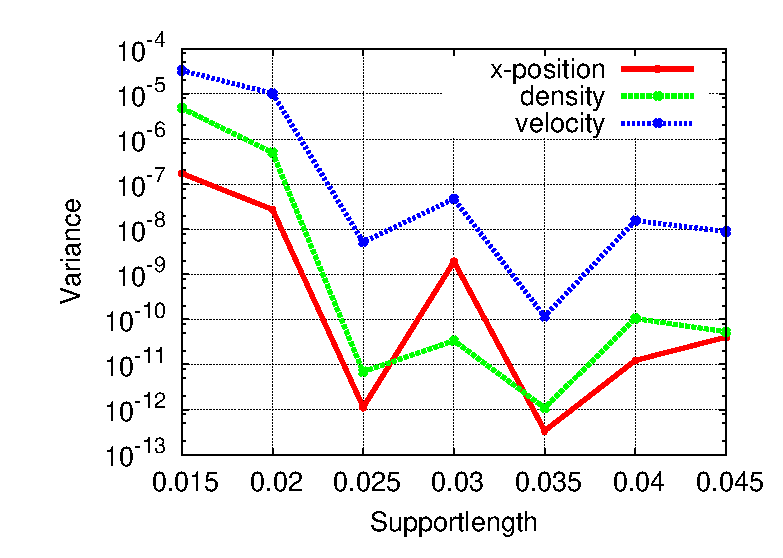
\includegraphics[width=7cm]{Graphics/results/ShockTube/q1D_CS_LF_SD/supLenVariat_dxdy005/Variance/VariancePart1}}
\subfigure[part 2]{
\label{fig:2DSPHresults_CS_varianceVersusSuplenPart2}
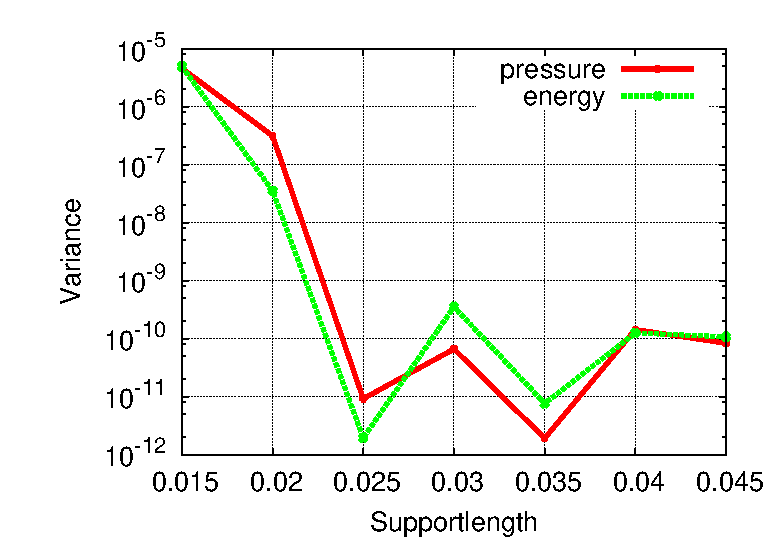
\includegraphics[width=7cm]{Graphics/results/ShockTube/q1D_CS_LF_SD/supLenVariat_dxdy005/Variance/VariancePart2}}

\caption[]{Evolution of variance with varying support length for all averaged quantities}

\end{figure}

This tendency of weakening with greater support length together with the fact that the particle drifting is symmetrical to the horizontal middle-line of the domain invokes the speculation that the non--uniformity in the second direction might be caused by the periodical boundary conditions in y--direction.


 
Despite of this change in properties in the second direction, the final results for the 1D shock--tube problem, i.\ e.\ the averaged values, are very accurate and totally comparable to the corresponding simulation simulation with purely 1D particle distribution. Sometimes (but rarely) the averaged 2D results are even more accurate.
Nevertheless the 2D particle distribution leads to slightly greater oscillations in the velocity profile than for the comparable 1D distribution.
 

   
\paragraph{1D constant mass particle distribution}
For the following set of simulations, all particles, no matter if LHS or RHS of the shock tube, have the same mass of $m=0.001875$ which results in a spacing on the LHS of $dx_l=0.001875$ and $dx_r=0.015$ on the RHS to reproduce the initial density values. 
The globally optimum support length for this configuration is 0.025 (figure (\ref{fig:2DSPHresults_1D_CM_dx_const}), but even in this case small oscillations are already present in the velocity profile after the shock--front. These oscillations get quickly bigger with even smaller support length and simultaneously the accuracy of the after shock-values deteriorates considerably, which can be seen clearly in the error evolution in area 3 in figure (\ref{fig:2DSPHresults_1D_CM_dx_const}). 
This is due to the insufficient number of neighboring particles in the RHS of the shock tube, where the particle distance is eight times higher than in the LHS. For a support length of 0.02 there are barely two neighboring particles which contribute to the interpolation on the RHS and for a support length of 0.015 there is just no neighbor any more and the interpolation is limited to the proper contribution of the particle itself, which is of course erroneous. 

The inaccuracy in the rarefaction, which was encountered for a constant spacing particle distributions both in 1D and 2D (see e.\ g.\ figure (\ref{figureBeiDT})) does not develop in the case of a 1D constant mass particle distribution. This might be the reason why 
in literature SPH shock--tube simulations are mostly found using the constant mass initialization approach \cite{Monaghan1983,Monaghan2005,Liu2003}, which also appears to be the physically more logical one.

For an example for the profiles of $\rho, p, u, e$ refer to figure (\ref{fig:1DSPHresults}) in the result section of the 1D code. 



\begin{figure}[H]
\centering
\label{fig:2DSPHresults_1D_CM_dx_const}

\subfigure[tight][whole domain]{
\label{fig:2DSPHresults_1D_CM_dx_const_wholeRho}
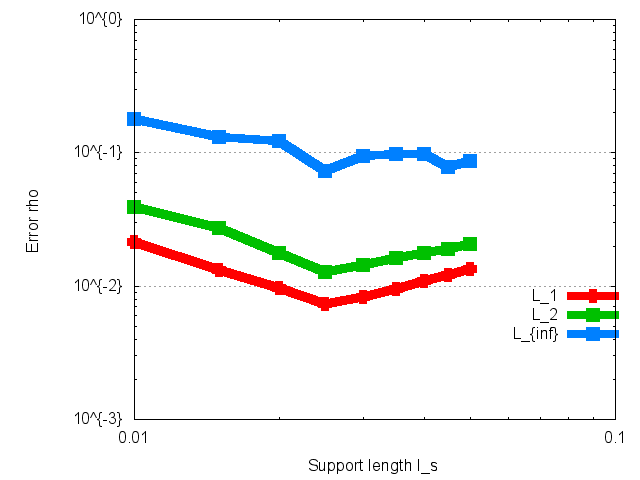
\includegraphics[width=5cm]{Graphics/results/ShockTube/1D_CM_LF_SD/supLenVariat_m001875/WholeDomainRho}}
\subfigure[tight][whole domain]{
\label{fig:2DSPHresults_1D_CM_dx_const_3Rho}
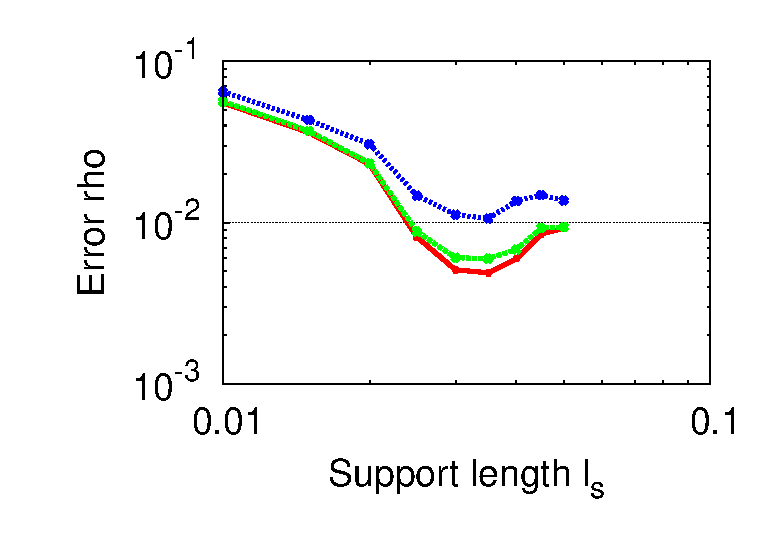
\includegraphics[width=5cm]{Graphics/results/ShockTube/1D_CM_LF_SD/supLenVariat_m001875/Area3Rho}}
\subfigure[tight][whole domain]{
\label{fig:2DSPHresults_1D_CM_dx_const_2Rho}
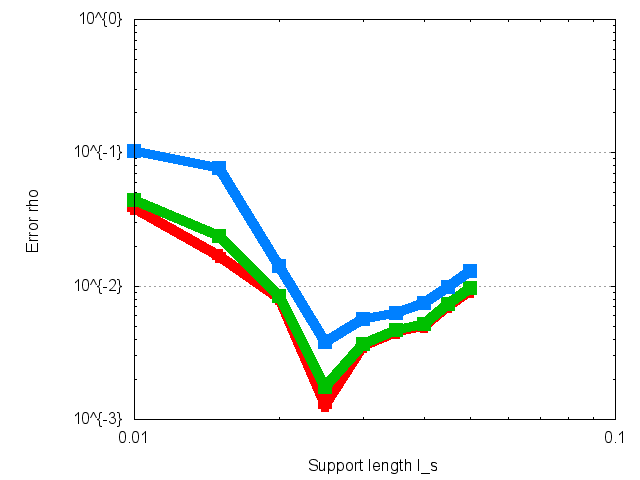
\includegraphics[width=5cm]{Graphics/results/ShockTube/1D_CM_LF_SD/supLenVariat_m001875/Area2Rho}}
\subfigure[tight][area 3]{
\label{fig:2DSPHresults_1D_CM_dx_const_wholeU}
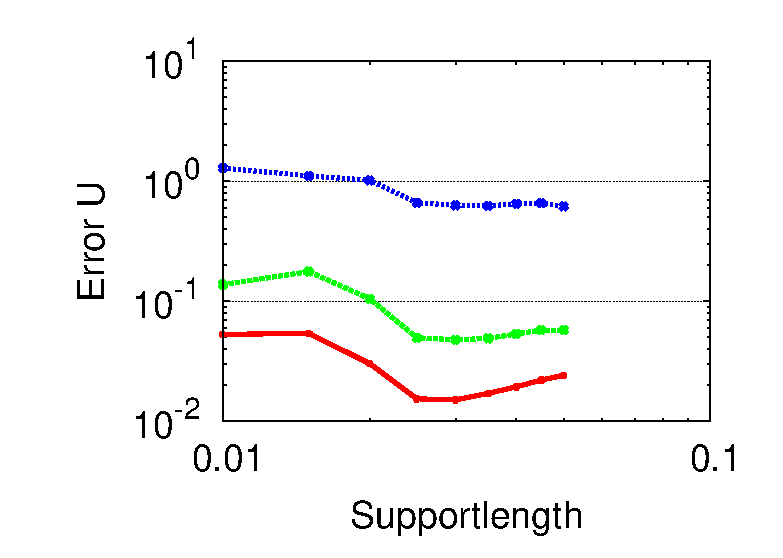
\includegraphics[width=5cm]{Graphics/results/ShockTube/1D_CM_LF_SD/supLenVariat_m001875/WholeDomainU}}
\subfigure[tight][area 3]{
\label{fig:2DSPHresults_1D_CM_dx_const_3U}
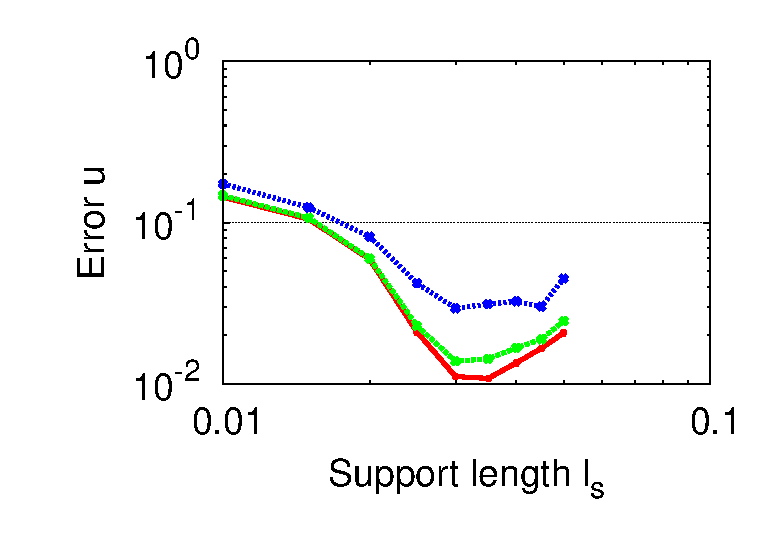
\includegraphics[width=5cm]{Graphics/results/ShockTube/1D_CM_LF_SD/supLenVariat_m001875/Area3U}}
\subfigure[tight][area 3]{
\label{fig:2DSPHresults_1D_CM_dx_const_2U}
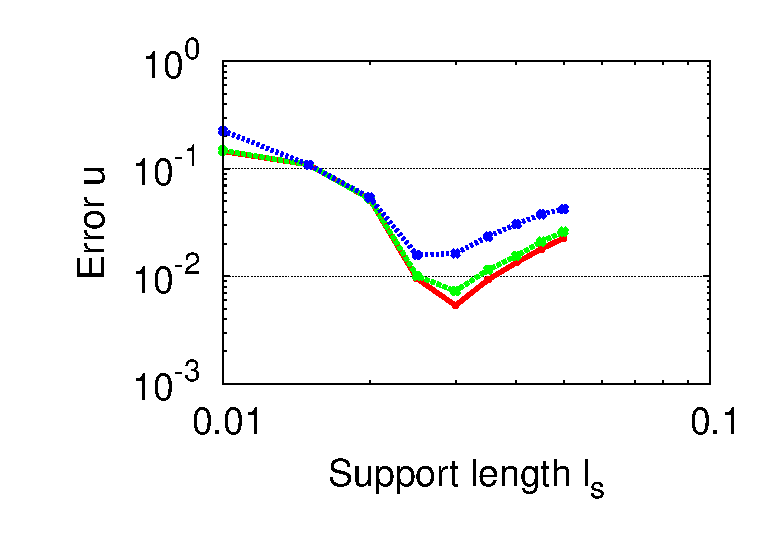
\includegraphics[width=5cm]{Graphics/results/ShockTube/1D_CM_LF_SD/supLenVariat_m001875/Area2U}}
\subfigure[tight][area 2]{
\label{fig:2DSPHresults_1D_CM_dx_const_wholeE}
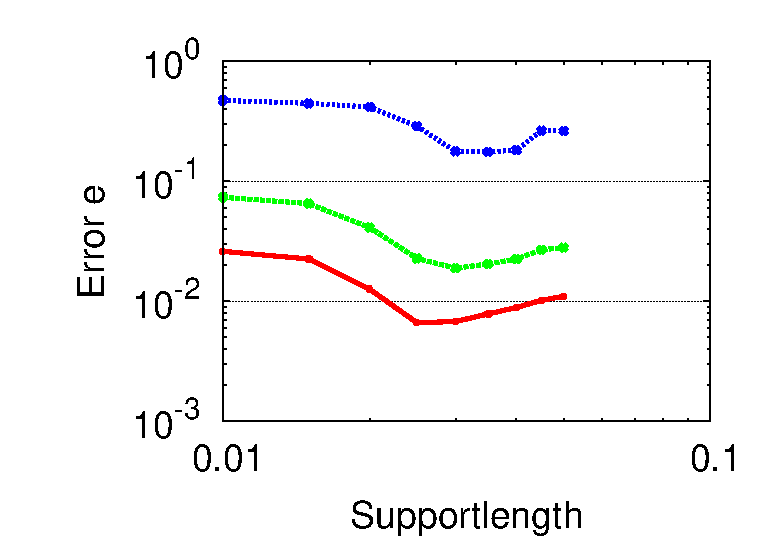
\includegraphics[width=5cm]{Graphics/results/ShockTube/1D_CM_LF_SD/supLenVariat_m001875/WholeDomainE}}
\subfigure[tight][area 2]{
\label{fig:2DSPHresults_1D_CM_dx_const_3E}
\includegraphics[width=5cm]{Graphics/results/ShockTube/1D_CM_LF_SD/supLenVariat_m001875/Area3E}}
\subfigure[tight][area 2]{
\label{fig:2DSPHresults_1D_CM_dx_const_2E}
\includegraphics[width=5cm]{Graphics/results/ShockTube/1D_CM_LF_SD/supLenVariat_m001875/Area2E}}

\caption[Convergence Shock-tube with 1D constant mass particle distribution]{L--norm errors of $\rho, u, e$ for a series of simulation with a varying support length and a constant particle spacing mass of $m=0.001875$ leading to a spacing on the LHS of $dx_l=0.001875$ and $dx_r=0.015$ on the RHS. The simulation is evaluated at $t=0.2$.}

\end{figure}

\paragraph{2D constant mass particle distribution}
The employed particle mass $m=2.5\cdot10^{-5}$ corresponds to a spacing of $dx_l=dy_l=0.005$ on the LHS and of $dx_r=dy_r=0.015$ on the RHS.
Simulations with this 2D constant mass particle distribution give the best results for a support length of $l_s=0.03$. However due to the discontinuity of the particle distribution in y--direction at the interface, there is a very weak drifting of the interface particles on the high density side in y--direction. This phenomenon increases with smaller support length - a tendency that has already been observed for the 2D constant spacing particle initialization. 
Besides, for most of the simulated cases there is again an inaccuracy in the velocity profile  within the rarefaction wave. The same has already been observed for 1D and 2D constant spacing initializations but not for 1D constant mass initializations.
The mentioned inaccuracy only disappears for support lengths  $l_s\geq0.4$.

The error evolution for the above discussed set of simulations can be found in the appendix, as there is no remarkable difference to the ones already shown. Due to the appearing inaccuracy in the rarefaction the figures look more like the ones from the constant spacing initialization than the one for 1D constant mass. 



\subsubsection{Resolution Study - ratio smoothing length/spacing held constant}
In this section, the resolution is gradually increased by simultaneously diminishing both the support length and the particle spacing in a way that their ratio remains constant. This means that the number of nearest neighbor particles remains constant. 
The convergence towards the exact solution is tested and the convergence ratio for each of the above mentioned four cases is determined. Having determined an optimum ratio of support length to particle spacing above, it is used here to obtain the highest possible accuracy for the simulation. In another set of simulations, at least for the purely 1D particle distributions, a non-optimum ratio is employed to verify the robustness of the method (kann man das sagen, ist das Robustness verification? Gibt es in der Numerik eine eigene, spezielle Definition von Robustness).

\paragraph{1D constant spacing particle distribution}
The simulations are conducted for a ratio of support length to particle spacing of 5 and the resolution is increased from a support length of 0.025 to 0.005, which corresponds to a number of particles from $N=401$ to $N=2001$. 
Figure (\ref{fig:2DSPHresults_1D_CS_ratioConst}) shows the quantitative evaluation of this set of simulation by means of the L-norm errors. The $L_1$ error shows roughly a first order convergence for all investigated quantities $\rho, u, e$ in all areas whereas the $L_2$ convergence is slightly lower.  (WARUM?)
The $L_{\inf}$ error of all quantities in the global domain are constant and caused by the non-discontinuous shock-resolution.

By the way, the inaccuracy in the rarefaction already encountered in section (\ref{sec:2DSPH_results_shock_resSTudy_dx=const}) for constant spacing particle distribution does not disappear but remains of about the same size, even for the highest resolution. 

%Außerdem, wie war das mit der Konvergenz? bei h/dx=const, convergierts dann gegen 0 oder bleibt ein resideller Fehler wegen Disktretisierungseffekt (dx). Müsste doch davon abhängen, on Diskretisierungsfehler von (h/dx) oder dx absolut abhängt!-->in verbindung dazu: kleine passage über fehler von SPH (dx, h) einfügen vorne


\begin{figure}[H]
\centering
\label{fig:2DSPHresults_1D_CS_ratioConst}

\subfigure[tight][whole domain]{
\label{fig:2DSPHresults_1D_CS_ratioConst_wholeRho}
\includegraphics[width=5cm]{Graphics/results/ShockTube/1D_CS_LF_SD/ratio_supLenDx5_dt0025/autom_dt_control/WholeDomainRho}}
\subfigure[tight][whole domain]{
\label{fig:2DSPHresults_1D_CS_ratioConst_3Rho}
\includegraphics[width=5cm]{Graphics/results/ShockTube/1D_CS_LF_SD/ratio_supLenDx5_dt0025/autom_dt_control/Area3Rho}}
\subfigure[tight][whole domain]{
\label{fig:2DSPHresults_1D_CS_ratioConst_2Rho}
\includegraphics[width=5cm]{Graphics/results/ShockTube/1D_CS_LF_SD/ratio_supLenDx5_dt0025/autom_dt_control/Area2Rho}}
\subfigure[tight][area 3]{
\label{fig:2DSPHresults_1D_CS_ratioConst_wholeU}
\includegraphics[width=5cm]{Graphics/results/ShockTube/1D_CS_LF_SD/ratio_supLenDx5_dt0025/autom_dt_control/WholeDomainU}}
\subfigure[tight][area 3]{
\label{fig:2DSPHresults_1D_CS_ratioConst_3U}
\includegraphics[width=5cm]{Graphics/results/ShockTube/1D_CS_LF_SD/ratio_supLenDx5_dt0025/autom_dt_control/Area3U}}
\subfigure[tight][area 3]{
\label{fig:2DSPHresults_1D_CS_ratioConst_2U}
\includegraphics[width=5cm]{Graphics/results/ShockTube/1D_CS_LF_SD/ratio_supLenDx5_dt0025/autom_dt_control/Area2U}}
\subfigure[tight][area 2]{
\label{fig:2DSPHresults_1D_CS_ratioConst_wholeE}
\includegraphics[width=5cm]{Graphics/results/ShockTube/1D_CS_LF_SD/ratio_supLenDx5_dt0025/autom_dt_control/WholeDomainE}}
\subfigure[tight][area 2]{
\label{fig:2DSPHresults_1D_CS_ratioConst_3E}
\includegraphics[width=5cm]{Graphics/results/ShockTube/1D_CS_LF_SD/ratio_supLenDx5_dt0025/autom_dt_control/Area3E}}
\subfigure[tight][area 2]{
\label{fig:2DSPHresults_1D_CS_ratioConst_2E}
\includegraphics[width=5cm]{Graphics/results/ShockTube/1D_CS_LF_SD/ratio_supLenDx5_dt0025/autom_dt_control/Area2E}}

\caption[Convergence Shock-tube 1D constant spacing particle distribution]{L--norm errors of $\rho, u, e$ for a series of simulation with increasing resolution and a constant ratio of support length to spacing of 5 evaluated at $t=0.2$.}

\end{figure}

\paragraph{2D constant spacing particle distribution}
Exactly like the corresponding 1D particle distribution, the 2D distribution showed optimum results for a ratio $h/dx=2.5$ ($l_s/dx=5$ KONTROLLIEREN) which is also taken for this set of simulations. The support length variation ranges from 0.025 to 0.005 which leads to a number of particles from $N=1995$ for the lowest resolution to $N=9995$ for the highest simulation. As for higher resolution not only the number of particles becomes higher but also the time step, which is coupled to $h$, becomes smaller, the time needed for the simulation increases considerably. %(2h30 on a seven year old ) computer for the highest resolution case)

The convergence behavior for this case of a 2D particle distribution with constant spacing is essentially the same as for the corresponding 1D case. i.\ e.\ about first order convergence. Therefore the graphical evaluation of the results is presented in the appendix.

In section (\ref{sec:2DSPH_results_shock_resSTudy_dx=const}), it has turned out that the 2D particle distribution result shows more velocity-oscillations in the aftershock area than one obtained with a 1D distribution. While these oscillations vanish for the 1D distribution with increasing resolution, they remain clearly visible in the velocity profile for the 2D distribution, even at the highest simulated resolution. They just become more and more confined to the area directly after the shock and at the contact discontinuity. 

 
\paragraph{1D constant mass particle distribution}
For the convergence test of the 1D constant mass particle distribution, a constant ratio $l_s/m=16$ has been taken, leading to ratios of $l_s/dx_l=RECHNEN$ on the LHS and $l_s/dx_r=RECHNEN$ on the RHS of the shock-tube problem. Again, the convergence rate is about first order as already for all cases before. The corresponding figure is shown in the Appendix. 

At the highest simulated resolution with $l_s=0.005$, corresponding to 3599 particles, the simulation result has a good quality. The shock is resolved very well, as its resolution scales with $l_s$ and the aftershock values are matched very accurately.

VIELLEICHT NOCHMAL DIE 4 BILDER VON EINER HOCHAUFLÖSENDEN SCHOCK-SIMULATION (WÄRE ABER ÄHNLICH ZU 1DSPH!!!)

AUẞERDEM KONVERGENZTEST NOCH FÜR NICHT-OPTIMALE RATIO SUPlEN/DX...->ROBUSTNESS


\paragraph{2D constant mass particle distribution}
Finally, the convergence of a 2D constant mass particle distribution has been examined using a constant ratio $l_s/\sqrt{m}=6$ found to be optimal in section (\ref{sec:2DSPH_results_shock_resSTudy_dx=const}) and a variation of $l_s$ from 0.3 to 0.1, corresponding to 3994 particles in the highest resolution.
The obtained convergence ratio is again around 1 order as can be seen from the figure in the Appendix. 

The inaccuracy in the rarefaction that has been observed in section (\ref{sec:2DSPH_results_shock_resSTudy_dx=const}) for a 2D constant mass particle distribution does not disappear with higher resolution. 
%vielleicht noch erwähnen dass eine weitere simulation durchgeführt wurde mit relativ größerer supLen (in Anlehnung an Resultate von 1D const mass distribution). i.\ e.\ ratio suplen/sqrt(m)=8 with supLen=0.01: Ergebnis: fehler in der rarefaktion ist weg! 
 

\subsubsection{Perturbation Study}
Beginning with an unperturbed particle distribution, the initial particle positions are more and more perturbed for subsequent simulations in a way explained in section (\ref{sec:2Dshock_simuSetup&Co}). To quantify the effect of this perturbation, the $L_1, L_2,$ and $L_{\infty}$ error--norms are evaluated. For each perturbation--factor, 5 different simulations with 5 newly generated particle distributions of this same perturbation factor are conducted and the error norms are averaged.


\paragraph{1D constant spacing particle distribution}
Generally a perturbed particle initialization leads to less smooth and results and profiles with many ``riffles''. As an example, the energy profiles of a heavily perturbed and an unperturbed simulation are shown in figure (\ref{fig:2DSPHresults_perturbationComparisonProfiles}).

\begin{figure}[!htbp]

\centering
\label{fig:2DSPHresults_perturbationComparisonProfiles}
\subfigure[]{
\label{{fig:2DSPHresults_perturbationComparisonProfiles_perturbed}}
\includegraphics[width=7cm]{Graphics/results/1DCode/velocity}}
\subfigure[]{
\label{fig:2DSPHresults_perturbationComparisonProfiles_UNperturbed}
\includegraphics[width=7cm]{Graphics/results/1DCode/density}}


\caption[Comparison of perturbed and unperturbed energy profiles]{Example of an energy profile obtained with a 1D constant spacing particle distribution for a simulation time of $t=0.2$: (\subref{fig:2DSPHresults_perturbationComparisonProfiles_perturbed}) initial particle distribution with a perturbation factor of $0.3$; (\subref{fig:2DSPHresults_perturbationComparisonProfiles_UNperturbed}) unperturbed particle initialization.}

\end{figure}

 The perturbation study based on a 1D constant mass particle distribution yields the following results (figure (\ref{fig:2DSPHresults_1D_CS_pertStudy})). Especially when looking at the after--shock and after--rarefaction areas, the effect of the perturbation can be noticed by principally increased  errors. In the whole domain, the general error, which is mainly due to the shock--resolution, is already so high that the additional relative error due to the perturbation is small.


\begin{figure}[H]
\centering
\label{fig:2DSPHresults_1D_CS_pertStudy}

\subfigure[tight][whole domain]{
\label{fig:2DSPHresults_1D_CS_pertStudy_wholeRho}
\includegraphics[width=5cm]{Graphics/results/ShockTube/PertStudy/basedOn1DconstSpace/WholeDomainRho}}
\subfigure[tight][whole domain]{
\label{fig:2DSPHresults_1D_CS_pertStudy_3Rho}
\includegraphics[width=5cm]{Graphics/results/ShockTube/PertStudy/basedOn1DconstSpace/Area3Rho}}
\subfigure[tight][whole domain]{
\label{fig:2DSPHresults_1D_CS_pertStudy_2Rho}
\includegraphics[width=5cm]{Graphics/results/ShockTube/PertStudy/basedOn1DconstSpace/Area2Rho}}
\subfigure[tight][area 3]{
\label{fig:2DSPHresults_1D_CS_pertStudy_wholeU}
\includegraphics[width=5cm]{Graphics/results/ShockTube/PertStudy/basedOn1DconstSpace/WholeDomainU}}
\subfigure[tight][area 3]{
\label{fig:2DSPHresults_1D_CS_pertStudy_3U}
\includegraphics[width=5cm]{Graphics/results/ShockTube/PertStudy/basedOn1DconstSpace/Area3U}}
\subfigure[tight][area 3]{
\label{fig:2DSPHresults_1D_CS_pertStudy_2U}
\includegraphics[width=5cm]{Graphics/results/ShockTube/PertStudy/basedOn1DconstSpace/Area2U}}
\subfigure[tight][area 2]{
\label{fig:2DSPHresults_1D_CS_pertStudy_wholeE}
\includegraphics[width=5cm]{Graphics/results/ShockTube/PertStudy/basedOn1DconstSpace/WholeDomainE}}
\subfigure[tight][area 2]{
\label{fig:2DSPHresults_1D_CS_pertStudy_3E}
\includegraphics[width=5cm]{Graphics/results/ShockTube/PertStudy/basedOn1DconstSpace/Area3E}}
\subfigure[tight][area 2]{
\label{fig:2DSPHresults_1D_CS_pertStudy_2E}
\includegraphics[width=5cm]{Graphics/results/ShockTube/PertStudy/basedOn1DconstSpace/Area2E}}

\caption[Perturbation influence shock-tube with 1D constant spacing particle distribution]{L--norm errors of $\rho, u, e$ for a series of simulation with increasing perturbation of initial particle position.}

\end{figure}


\paragraph{2D constant spacing particle distribution}


\paragraph{1D constant mass particle distribution}

In section (\ref{sec:2Dshock_simuSetup&Co}) it was mentioned that the mass initialization of the particles for the resolution study is done employing the SPH interpolation formula, contrary to all the shock-tube results presented in previous sections, where mass was initialized in 1D according to $m=\rho dx$ and in 2D $m=\rho dx dy$. While this makes no difference for a constant spacing initialization, the use of the 
kernel interpolation leads to a relatively strong irregularity in the mass profile close to the contact discontinuity (CD) if the particles are distributed according to a constant mass initialization. This  influences the simulation result compared to an initialization using $m=\rho dx dy$ and leads to higher errors.  

\begin{table}[h] % in eckigen Klammern steht die Platzierung, h steht f�r genau hier
\label{tab:2D_shock_m_smoothed_versus_rhodx}
\centering

\begin{tabular}[c]{|l| c|l| c|l| c|} % die eckige Klammer steht f�r die Ausrichtung der Tabelle im Text: c steht f�r zentriert
\hline
\hline
\multicolumn{2}{|c|}{\textbf{$L_1$--error}} & \multicolumn{2}{|c|}{\textbf{$L_2$--error}} & \multicolumn{2}{|c|}{\textbf{$L_{\infty}$--error}}\\
\hline
smoothed & $\rho dx$ & smoothed & $\rho dx$& smoothed & $\rho dx$\\
\hline
\hline
length & $l$ & meter & $m$ & length & {\bf L}\\

mass & $m$ & kilogram & $kg$ & mass & {\bf M} \\

time & $t$ & second & $s$ & time & {\bf T}\\

\hline
\hline
\end{tabular}
\caption[]{Comparisons of error values for simulations with an unperturbed constant mass particle distribution for the two mass initialization methods smoothing and $\rho dx$.}

\end{table}

In the case of the 1D constant mass initialization the effect of a perturbed particle position is visible in figure (\ref{fig:2DSPHresults_1D_CM_pertStudy}). 
Especially for the after--shock (area 2) and after--rarefaction (area 2) values a clear and monotonous increase in the error can be observed. Again the level of the global error, which is mainly due to the non-discontinuous shock resolution, is already relatively high compared to the error induced by the particle disorder. Thus the latter can be perceived only weakly considering the whole domain.
\begin{figure}[H]
\centering
\label{fig:2DSPHresults_1D_CM_pertStudy}

\subfigure[tight][whole domain]{
\label{fig:2DSPHresults_1D_CM_pertStudy_wholeRho}
\includegraphics[width=5cm]{Graphics/results/ShockTube/PertStudy/basedOn1DconstMass/WholeDomainRho}}
\subfigure[tight][whole domain]{
\label{fig:2DSPHresults_1D_CM_pertStudy_3Rho}
\includegraphics[width=5cm]{Graphics/results/ShockTube/PertStudy/basedOn1DconstMass/Area3Rho}}
\subfigure[tight][whole domain]{
\label{fig:2DSPHresults_1D_CM_pertStudy_2Rho}
\includegraphics[width=5cm]{Graphics/results/ShockTube/PertStudy/basedOn1DconstMass/Area2Rho}}
\subfigure[tight][area 3]{
\label{fig:2DSPHresults_1D_CM_pertStudy_wholeU}
\includegraphics[width=5cm]{Graphics/results/ShockTube/PertStudy/basedOn1DconstMass/WholeDomainU}}
\subfigure[tight][area 3]{
\label{fig:2DSPHresults_1D_CM_pertStudy_3U}
\includegraphics[width=5cm]{Graphics/results/ShockTube/PertStudy/basedOn1DconstMass/Area3U}}
\subfigure[tight][area 3]{
\label{fig:2DSPHresults_1D_CM_pertStudy_2U}
\includegraphics[width=5cm]{Graphics/results/ShockTube/PertStudy/basedOn1DconstMass/Area2U}}
\subfigure[tight][area 2]{
\label{fig:2DSPHresults_1D_CM_pertStudy_wholeE}
\includegraphics[width=5cm]{Graphics/results/ShockTube/PertStudy/basedOn1DconstMass/WholeDomainE}}
\subfigure[tight][area 2]{
\label{fig:2DSPHresults_1D_CM_pertStudy_3E}
\includegraphics[width=5cm]{Graphics/results/ShockTube/PertStudy/basedOn1DconstMass/Area3E}}
\subfigure[tight][area 2]{
\label{fig:2DSPHresults_1D_CM_pertStudy_2E}
\includegraphics[width=5cm]{Graphics/results/ShockTube/PertStudy/basedOn1DconstMass/Area2E}}

\caption[Perturbation influence shock-tube with 1D constant mass particle distribution]{L--norm errors of $\rho, u, e$ for a series of simulation with increasing perturbation of initial particle position}

\end{figure}

\paragraph{2D constant mass particle distribution}
DONE -- NOT YET INTEGRATED IN REPORT




\subsection{1D Linear acoustic waves}
\label{sec:Results_1DLinearAcousticWaves}
The ability of the SPH code to handle acoustic waves is tested by three simulation setups as introduced in section (\ref{sec:AcousticWavePropagation_GenIntro}). 



\subsubsection{1D oscillating wave}
\label{sec:Results_1DoscillatingWave}
The simulations are conducted with a domain of unit size and $N=100$ equi--spaced particles, leading to a spacing of $dx=0.01$ as used by Monaghan \cite{Monaghan2005}.
In a first step, artificial viscosity is globally included in the simulation, i.\ e.\ unlike for the shock--tube simulation it is active both in compression zones and in rarefactions. 

Different support lengths are employed to analyze a potential influence of this parameter on the quality of the results.

 Figure (\ref{fig:Results_1DoscillatingWave_supLen03}) shows the damping factor according to equation (\ref{eq:DampingFactor}) and the temporal evolution of the periodical time $T$ for a support length of $l_s=0.03$. It can be observed, that neither the damping factor nor $T$ remain temporally constant, which therefore does not correspond to an accurate solution.  

\begin{figure}[h]
 \label{fig:Results_1DoscillatingWave_supLen03}
\centering
\subfigure[Evolution of damping factor]{
\includegraphics[width=7cm]{Graphics/results/1DWave/Oscillation/WithGlobalArtVisSupLen030/DampingFactor}
}
\subfigure[Evolution of periodical time]{
\includegraphics[width=7cm]{Graphics/results/1DWave/Oscillation/WithGlobalArtVisSupLen030/Period}
}
\caption[1D Oscillation: Damping factor and periodical time for $l_s/dx=3$]{Temporal evolution of the damping factor and the periodical time for a stationary oscillation simulated with $dx=0.01$ and a support length of $l_s=0.03$. Artificial viscosity is taken into account for zones in compression and rarefactions.}

\end{figure}

In an attempt to find more accurate results, the evolution of the periodical time $T$ with varying $l_s/dx$ has been studied. It made no essential difference if $dx$ was varied with constant $l_s$ or opposite, thus confirming that the influence parameter would be the ratio $l_s/dx$ and not one of the values separately. Indeed, the results of this study yield a significant dependence of the periodical time on this parameter, as can be seen in figure (\ref{fig:Results_1DoscillatingWave_T_versus_ls/dx}). For very low ratios $l_s/dx$ the support domain is simply to small for the given particle spacing and thus, the high error is not surprising. However in the area of $l_s/dx\approx2$ to $l_s/dx\approx3.5$, where reasonable SPH simulations are possible, there are still values which produce a significantly erroneous periodical time. 
At first sight there seem to be several ratios $l_s/dx$ which lead to accurate results. This however is only in terms of the periodical time. When additionally the damping is included in the judgment, only the value $l_s/dx=2.52$ has a constant damping factor. All the other values that resulted in correct periodical times had non--constant damping factors, with partly significant variations. Besides, these cases showed a distorted wave shape %possibly due to the SPH dispersion???
after a couple of periods, while for $l_s/dx=2.52$ the shape remained essentially unchanged as well. 



\begin{figure}[h]
 \label{fig:Results_1DoscillatingWave_T_versus_ls/dx}
\centering

\includegraphics[width=7cm]{Graphics/results/1DWave/Oscillation/suplen_influence}

\caption[1D Oscillation: periodical time versus $l_s/dx$]{Influence of the ratio $l_s/dx$ on the accuracy of the periodical time. The theoretically exact value %for the linear theory
is $T=0.84515$. %the underlying simulations have been conducted with artificial viscosity globally turned on.
}

\end{figure}

The retained value for the ratio support length to particle spacing for the further acoustic wave simulations is therefore $l_s/dx=2.52$, which gives accurate and constant results both for the periodical time and the damping (see figure (\ref{fig:Results_1DoscillatingWave_supLen0252})). By the way this optimum is quite close to the value $l_s/dx02.6$ used by Monaghan for his dispersion study \cite{Monaghan2005} although even for the Monaghan value an error in the periodical time of 2.5\% was found. 

On the other hand Monaghan stated in an earlier publication \cite{Monaghan1992} that better results for acoustic waves can be obtained with integer ratios $h/dx$, that means even integer ratios $l_s/dx$. Indeed, this is true in terms of periodical time (figure (\ref{fig:Results_1DoscillatingWave_T_versus_ls/dx})) but as mentioned above, the damping, in case there is a viscosity, would not be accurate.

\begin{figure}[h]
 \label{fig:Results_1DoscillatingWave_supLen0252}
\centering
\subfigure[Evolution of damping factor]{
\includegraphics[width=7cm]{Graphics/results/1DWave/Oscillation/withGlobalArtVisSupLen0252/DampingFactor}
}
\subfigure[Evolution of periodical time]{
\includegraphics[width=7cm]{Graphics/results/1DWave/Oscillation/withGlobalArtVisSupLen0252/Period}
}
\caption[1D Oscillation: Damping factor and periodical time for $l_s/dx=2.52$]{Temporal evolution of the damping factor and the periodical time for a stationary oscillation simulated with $dx=0.01$ and a support length of $l_s=0.0252$. Artificial viscosity is taken into account for zones in compression and rarefactions.}

\end{figure}

Furthermore the influence of artificial viscosity on the damping is tested. Without any artificial viscosity, there is no observable damping, as can be seen on the velocity amplitude in figure (\ref{fig:Results_1DoscillatingWave_u_profiles_wo_artVisc}) . Thus, the SPH method does not produce any intrinsic numerical dissipation. The results without any viscosity however is very sensitive to any (even numerical) perturbation, as these are not dampened at all. Therefore the oscillating wave looses its perfectly sinusoidal shape after some periods. If the artificial viscosity is included in the simulation, these omnipresent little perturbations are immediately dampened and have no effect on the shape of the oscillating wave.

\begin{figure}[h]
 \label{fig:Results_1DoscillatingWave_u_profiles}
\centering
\subfigure[Without artificial viscosity]{
\label{fig:Results_1DoscillatingWave_u_profiles_wo_artVisc}
\includegraphics[width=7cm]{Graphics/results/1DWave/Oscillation/withoutArtVisSupLen0252/ShapeChangeV}
}
\subfigure[Including artificial viscosity]{
\label{fig:Results_1DoscillatingWave_u_profiles_w_artVisc}
\includegraphics[width=7cm]{Graphics/results/1DWave/Oscillation/withGlobalArtVisSupLen0252/ShapeChangeV}
}
\caption[Velocity profiles 1D oscillation]{Velocity profiles at the beginning of the simulation and after 10 periods: \subref{fig:Results_1DoscillatingWave_u_profiles_wo_artVisc} without any artificial viscosity, \subref{fig:Results_1DoscillatingWave_u_profiles_w_artVisc} including a global artificial viscosity, which is effective for compression zones as well as for rarefactions. Both simulations are conducted with $l_s/dx=2.52$.}

\end{figure}

The effect of the artificial viscosity on the velocity amplitude of the oscillation is significant and can be quantified by the damping factor, which is $c_d=0.107$ in the case of a globally active artificial viscosity. The effect of the damping on the velocity profile of the oscillation is presented in figure (\ref{fig:Results_1DoscillatingWave_u_profiles_w_artVisc}). One way to reduce the damping for the oscillating wave, is an artificial viscosity that is only active in compression zones, as it was used for the shock--tube simulations. Thus, the damping factor can essentially be reduced by a factor 2. As will be shown later, this does not work for traveling waves without any side effects. 
A more appropriate way of reducing artificial viscosity in zones where it is not needed is therefore suggested by \cite{Monaghan2005}.



\subsubsection{1D traveling wave}

The same optimum ratio $l_s/dx=2.52$, which has been found in section (\ref{sec:Results_1DoscillatingWave}) for the oscillating wave, also applies for the traveling wave, thus giving again virtually the exact value of $T=0.84515$. 

The influence of artificial viscosity on the traveling wave is subject of the following passage.

While the velocity profile of the stationary oscillation without any artificial viscosity became quickly perturbed as an effect of (numerical )perturbations, the traveling wave seems to be more resistant to this phenomenon. Its velocity profile only shows a slight deviation of the original shape in figure (\ref{fig:Results_1DoscillatingWave_u_profiles_wo_artVisc}). The same figure confirms again that there is no intrinsic numerical dissipation as the peak velocity remains unchanged.

Including the global artificial viscosity, the damping is clearly visible, as shown in figure (\ref{fig:Results_1DTravelingWave_u_profiles_w_artVisc}). If, as an attempt to reduce damping, the artificial viscosity is turned off for rarefactions and thus only taken into account in compression zones, there is now a side--effect as visible in figure (\ref{fig:Results_1DTravelingWave_u_profiles_w_artViscCompr}). Unlike for the stationary oscillation, the wave shape becomes seriously distorted for the traveling wave. This can easily be explained by symmetry. The sides of the antinode of a stationary oscillation consist either both of compression or both of expansion zones thus always leading to a symmetrical situation relative to the center of the antinode. It therefore does not matter for the shape of the oscillation, whether artificial viscosity only acts for compressions or for expansions as well.

 A wave crest or wave trough of a traveling wave whereas consists always of one compression and one expansion zone, thus leading to an asymmetrical situation if artificial viscosity only acts for compressions. In figure (\ref{fig:Results_1DTravelingWave_u_profiles_w_artViscCompr}) for example where the wave is traveling from left to right, the areas $0\leq x <0.25$ and $0.75\leq x \leq 1$ are zones in compression and therefore flattened due to the artificial viscosity. The zone $0.25\leq x <0.75$ is in expansion and therefore untouched by the artificial viscosity.
As already mentioned for the 1D oscillation this switching off artificial viscosity for expansion zones is therefore not an appropriate way of reducing artificial viscosity if traveling acoustic waves are present.

\begin{figure}[h]
 \label{fig:Results_1TravelingWave_u_profiles}
\centering
\subfigure[Without artificial viscosity]{
\label{fig:Results_1DTravelingWave_u_profiles_wo_artVisc}
\includegraphics[width=7cm]{Graphics/results/1DWave/TravelingWave/withoutArtViscSupLen0252/ShapeChangeV}
}
\subfigure[Including global artificial viscosity]{
 \label{fig:Results_1DTravelingWave_u_profiles_w_artVisc}
\includegraphics[width=7cm]{Graphics/results/1DWave/TravelingWave/withGlobalArtViscSupLen0252/ShapeChangeV}
}
\subfigure[Including artificial viscosity for compression only]{
 \label{fig:Results_1DTravelingWave_u_profiles_w_artViscCompr}
\includegraphics[width=7cm]{Graphics/results/1DWave/TravelingWave/WithArtViscForComprSupLen0252/ShapeChangeV}
}
\caption[Velocity profiles 1D traveling wave]{Velocity profiles at the beginning of the simulation and after 10 periods: \subref{fig:Results_1DTravelingWave_u_profiles_wo_artVisc} without any artificial viscosity, \subref{fig:Results_1DTravelingWave_u_profiles_w_artVisc} including a global artificial viscosity, which is effective for compression zones as well as for rarefactions and \subref{fig:Results_1DTravelingWave_u_profiles_w_artViscCompr} including artificial viscosity for zones in compression only.}

\end{figure}


\subsubsection{1D wave train with reflection and interference}
This test case aims at showing qualitatively the ability of the code to deal with reflections and interferences. The latter should work naturally as it only constitutes a superposition of two waves. But the reflection can be seen as a first challenge for the solid wall boundary condition method as used for the domain edges.
The simulated situation is described in detail in section (\ref{sec:GenIntro_1DWaveTrainReflect}). Figure (\ref{fig:Results_1DWaveTrainReflect_u_profiles}) presents the velocity field of the domain at various instants during a simulation without artificial viscosity.

\begin{figure}[h]
 \label{fig:Results_1DWaveTrainReflect_u_profiles}
\centering
\subfigure[at $t=\frac{t_1}{2}=0.2113$]{
\label{fig:Results_1DWaveTrainReflect_u_profiles1}
\includegraphics[width=7cm]{Graphics/results/1DWave/SingleWaveTrainReflect/Velocity00211000}
}
\subfigure[at $t=1.4790$]{
 \label{fig:Results_1DWaveTrainReflect_u_profiles2}
\includegraphics[width=7cm]{Graphics/results/1DWave/SingleWaveTrainReflect/Velocity01478999}
}
\subfigure[at $t=2.1129$]{
 \label{fig:Results_1DWaveTrainReflect_u_profiles3}
\includegraphics[width=7cm]{Graphics/results/1DWave/SingleWaveTrainReflect/Velocity02112999}
}
\subfigure[at $t=2.7468$]{
 \label{fig:Results_1DWaveTrainReflect_u_profiles4}
\includegraphics[width=7cm]{Graphics/results/1DWave/SingleWaveTrainReflect/Velocity02746999}
}

\caption[Velocity profiles 1D reflected wave train]{Velocity profiles for the simulated situation as described in section (\ref{sec:GenIntro_1DWaveTrainReflect}) at various instants and without artificial viscosity: \subref{fig:Results_1DWaveTrainReflect_u_profiles1}: half the wave train has already been generated by the moving wall \subref{fig:Results_1DWaveTrainReflect_u_profiles2}: short before the wave hits the RHS wall, \subref{fig:Results_1DWaveTrainReflect_u_profiles3}: after entire reflection at the RHS wall and after generation of a new wave train at the LHS wall. \subref{fig:Results_1DWaveTrainReflect_u_profiles4}: at maximum interference}

\end{figure}

The results look qualitatively as expected, although the wave shape degrades during the course of the simulation. This however is again due to the absence of artificial viscosity. Perturbations, here probably mainly due to the wall movement, are not dampened but can evolve and thus influence the wave shape. 
Roughly comparing the amplitudes of figures (\ref{fig:Results_1DWaveTrainReflect_u_profiles1}) and (\ref{fig:Results_1DWaveTrainReflect_u_profiles3}) shows that the amplitude is about conserved by the reflection, biased by the perturbation of the wave shape. A more accurate way of assessing the absence of dissipation would be the computing of the kinetic energy content of the wave at both instants.  
A similar rough estimation can be done for the instant of maximum interference shown in figure (\ref{fig:Results_1DWaveTrainReflect_u_profiles4}) with the result that the amplitude is about twice as big as the one of the single wave. 




A simulation including artificial viscosity has been performed as well. In this case the wave maintains its shape, confirming the above statement that the shape change for the wave without artificial viscosity is due to the non--damping of perturbations. 
The amplitude of the wave however is dampened that much that after traveling back and forth through the domain, it is dissipated almost completely.


%..\cite{Monaghan1992}: good agreement with theory if wavelength $\lambda > 2\pi h$. Besides better results (particularly in terms of propagation speed), if $\Delta x=1$ or $\Delta x=2$ than with $\Delta x=1.5$


\subsection{Taylor--Green flow}
\label{sec:Results_TG}

The Taylor--Green flow is the first real 2D simulation setup and tests the viscosity implementation. All simulations are conducted with particle properties and settings according to section (\ref{sec:SimuSetup_TG}). Unless other wise stated, the number of particles used is $N=3600$ resulting in a particle spacing of $dx=dy=0.0167$. In a first step, the support length is chosen to $l_s=2dx$ as it was done by \cite{Hu2007} for their Taylor--Green simulation. %habe gecheckt, der von denen verwendete quintic spline hat auch l_s=2h! 

Based on information found in literature \cite{Chaniotis2002, Ellero2007} the first simulation attempts are conducted for low Reynolds numbers. For, it has been reported that higher Reynolds numbers, where the particles move away from their initial positions considerably before the velocity has entirely decayed, may lead to inaccuracies in the results. $Re$ is changed by varying the viscosity value.

For a  Reynolds number of $Re=10^{-2}$ for example, the particle positions remain virtually unchanged during the entire simulation. The initial velocity field of the Taylor--Green simulation is presented in figure (\ref{fig:Results_TG_initvelocit}). The temporal decay of the simulation as well as the error relative to the incompressible reference solution are shown in figure (\ref{fig:Results_TG_VelocDecay_Re0_01_l_s_2dx}). The error in maximum velocity at the instant $t_{50}$  where the velocity has decayed to $1/50$ of the initial value is $38.9\%$. For a basic SPH code without any special corrections, this is an acceptable value as errors in the same order of magnitude were found by \cite{Hu2007}.

\begin{figure}[h]
 \label{fig:Results_TG_initvelocity}
\centering
\includegraphics[width=7cm]{Graphics/results/TaylorGreen/N3600_eta_100_suplen2dx/InitVeloc}
\caption[Velocity field Taylor--Green]{Initial velocity field for the Taylor--Green flow. Also included is the initial particle distribution for the case of $N=3600$ particles.}
\end{figure}

\begin{figure}[h]
\centering
\label{fig:Results_TG_VelocDecay_Re0_01}
\subfigure[support length $l_s=2dx$]{
 \label{fig:Results_TG_VelocDecay_Re0_01_l_s_2dx}
\includegraphics[width=7cm]{Graphics/results/TaylorGreen/N3600_eta_100_suplen2dx/VelocDecay}
}
\subfigure[support length $l_s=4dx$]{
\label{fig:Results_TG_VelocDecay_Re0_01_l_s_4dx}
\includegraphics[width=7cm]{Graphics/results/TaylorGreen/N3600_eta_100_suplen4dx/VelocDecay}
}
\caption[Velocity decay Taylor--Green at $Re=0.01$]{Temporal decay of the velocity for a Taylor--Green simulation with $N=3600$ particles, $Re=0.01$ and different support lengths. The line labeled ``Exact'' is the analytical incompressible reference solution.}
\end{figure}

A considerable improvement of the results can be achieved by using a support length of $l_s=4dx$. The higher support length seems to reduce the effective viscosity and leads to a slower decay which matches better the reference solution as can be seen in figure (\ref{fig:Results_TG_VelocDecay_Re0_01_l_s_4dx}). At $t_{50}$, the error is now $14.3\%$.



For higher Reynolds numbers, the above mentioned effect of particle movement influences the quality of the results. The particle field becomes distorted and thus causes errors. A Reynolds number of $Re=1$ still produces acceptable results with an error at $t_{50}$ of $L_{\infty,50}\approx37\%$. The particle field of this simulation is already considerably distorted, but the structured particle arrangement is maintained until complete decay of the velocity. With even higher Reynolds numbers, the structured particle arrangement dissolves completely, leading to entirely unphysical simulation results. The described phenomenon can be observed for a $Re=100$ for example, For this case, figure (\ref{fig:results_TG_Re100_Positions_distorted}) shows the distorted but still structured particle field and figure (\ref{fig:results_TG_Re100_Positions_unstructured}) the field after the structure has dissolved. The dissolved particle field shows no homogeneous disorder but bunches of particles arranged in little line fragments. The same, phenomenon, even though less intense was observed by \cite{Ellero2007}. In their case however the number of particles was $N=10000$ and therefore about three times higher, which could explain the better homogeneity.

\begin{figure}[h]
\label{fig:results_TG_Re100_Positions}
\subfigure[at $t=$]{
\label{fig:results_TG_Re100_Positions_distorted}

\includegraphics[width=7cm]{Graphics/results/TaylorGreen/N3600_eta_0_01_suplen4dx/distorted}
}
\subfigure[at $t=$]{
\label{fig:results_TG_Re100_Positions_unstructured}

\includegraphics[width=7cm]{Graphics/results/TaylorGreen/N3600_eta_0_01_suplen4dx/unstructured}
}
\caption[Particle positions for Taylor--Green at $Re=100$]{Particle positions at different instants for a Reynolds number of $Re=100$. The number of particles is $N=3600$. \subref{fig:results_TG_Re100_Positions_distorted}: distorted but still structured particle field. \subref{fig:results_TG_Re100_Positions_unstructured}: particle field after the structure has dissolved.} 
\end{figure}

One way of reducing the errors induced by the disordering of the particle arrangement is starting the simulation from a so called relaxed particle field \cite{Ellero2007}. It can be obtained by running a previous simulation to the point of complete dissolution of particle structure and then re--initializing this field with the initial properties of a Taylor--Green vortex. 



The influence of spatial resolution on the Taylor--Green results is investigated for a Reynolds number of $Re=10^{-2}$ in order to avoid the effect of particle movement. A support length of $l_s=2dx$ is chosen for this set of simulations as it showed higher errors tah a bigger value. Finally, the results of the convergence study for this configuration are surprising as can be seen from figure. (\ref{fig:Results_TG_Resolution}). There is a virtually constant residual error of around $38\%$ no matter which resolution. A first idea was that this residual error could be due to compressibility error as the simulation is compared to an incompressible reference. But even with a new simulation neglecting the viscous heating term in the energy equation no change in results have been noticed. Another reason for this residual error, which again is speculation, could be the discretization approximation error, which depends on $l_s/dx$. Perhaps this error is very predominant for this particular configuration? 


\begin{figure}[h]
 \label{fig:Results_TG_Resolution}
\centering
\includegraphics[width=7cm]{Graphics/results/TaylorGreen/Eta_100_suplen2dx_ResStudy/ErrorResolution}
\caption[Convergence Taylor--Green]{Convergence behavior of a Taylor--Green flow with a Reynolds number of $Re=100$.}
\end{figure}


\subsection{Pure Heat--Conduction  -- Slab with temperature jump}

The pure heat conduction test--case is not a flow problem but rather models a solid object where only the evolution of temperature is simulated. 

In a first step, the time step limitation criterion due to thermal conduction is verified. Subsequently the slab is tested with both adiabatic and isothermal boundary conditions. 

\subsubsection{Verification of time step--condition for conduction}
%Noch überlegen in welche sub oder subsub section dieser Schritt kommt.Denn eigentlich gehört er unter adiabatic slab, da dies die simulierte Konfiguration ist, allerdings ist die Verifikation allgemeingültig gedaxht, d.h auch z.b für isothermal slab. Dies würde dafür sprechen, ein extra kapitel aufzumachen. Und zwar am Anfang von Heatconduction wäre am logischsten (da bevor eigentlich simuliert wird, dt getestet werden müsste müsste...)

Based on a setup with adiabatic boundary condition used in the following paragraph (\ref{sec:Results_PureHeat_adiabaticBC}), the correctness of the
heat conduction-related time stepping criterion expressed in equation (\ref{eq:dt_limitation_thermal}) ist tested. The simulation errors, conducted with different time steps, are compared at a simulation time of 1. 
%although the error (due to spatial discretization) is max. at much smaller times) but I wanted to give a potental temporal error some tie to evolve. 
%EVTL. RESOLUTION STUDY DESWEGEN NCIHMAL MACHEN UND ZWAR FÜR JEDE SUPLEN MIT IHREM OPTIMALEN TIMESTEP! VIELLECIHT ERKLÄRT DISEE TATSACHE DASS DIE KONVERENZ NICHT SO ``GLATT'' IST...


\begin{figure}[h]  
  \label{fig:PureHeat_dtVerification}
  \centering
  \includegraphics[width=7cm]{Graphics/results/PureHeatConduction/ErrorTimestep}
  \caption{Evolution of the error after at $t=1.25$ with a variation of time step}
\end{figure}

Figure \ref{fig:PureHeat_dtVerification} shows that there is a real optimum, i.\ e.\ slight deterioration of the results when the employed timestep $dt$ is inferior to the optimum timestep $dt_\mathit{opt}$. %According to \cite{Cleary1999}, more details on time stepping for a pure conduction problem can be found in \cite{} (could not access article yet).%(somehow strange that results get worse if dt diminishes???, does this have to do with the initial discontinuity or is this a normal behavior?????)
It is remarkable that such an optimum exists, as this might have effects on the use of the heat conduction model in a combined flow and conduction simulation. Then, there are several time step limitations and it is not guaranteed that the one chosen is always the optimum one for thermal conduction. The results might therefore not have the optimum accuracy. In Cleary \cite{Cleary2002}, where this model is applied to a flow problem including heat conduction, this effect is not taken into account, as time is only limited by a combined Courant and viscosity condition.

%Problems also for flow simulation, when several time stepping criteria apply and in general dt $<$ (sometimes even dt$<<$) $dt_\mathit{opt}$ for heat conduction! Have a look at literature (e.\ g.\ Cleary2002, where the heat conduction model is applied to flows: nothing new: only uses CFL incl. viscosity, (which is dominant by far probably versus thermo...)).Not

\subsubsection{Slab with temperature jump and adiabatic boundary conditions}
\label{sec:Results_PureHeat_adiabaticBC}

The slab with a LHS temperature $T_l=0$ and a RHS temperature of $T_r=1$ has symmetry boundary conditions in x--direction, which lead to adiabatic slab edges.
According to Cleary \cite{Cleary1999}, a support length of $l_s=2dx$is used for all simulations in this section .

First, the correctness of the implemented conduction model is tested in the initial phase, where the solution can be compared to the reference given in (\ref{eq:Two_SemiInfBodies}) and where therefore the boundary conditions do not play any role.

Figure (\ref{fig:PureHeat_T_profilesInitialPhase}) shows the temperature profile at different instants.

\begin{figure}[!htbp]
\centering
\label{fig:PureHeat_T_profilesInitialPhase}
\subfigure[at $t=0.1$]{
\label{fig:PureHeat_T_profilesInitialPhase0.1}
\includegraphics[width=7cm]{Graphics/results/PureHeatConduction/T_profiles000000100000}}
\subfigure[at $t=1.0$]{
\label{fig:PureHeat_T_profilesInitialPhase1}
\includegraphics[width=7cm]{Graphics/results/PureHeatConduction/T_profiles000001000000}}
\subfigure[at $t=2.0$]{
\label{fig:PureHeat_T_profilesInitialPhase2}
\includegraphics[width=7cm]{Graphics/results/PureHeatConduction/T_profiles000002000000}}
\subfigure[at $t=4.0$]{
\label{fig:PureHeat_T_profilesInitialPhase4}
\includegraphics[width=7cm]{Graphics/results/PureHeatConduction/T_profiles000003999999}}

\caption[Temperature profiles at the initial phase of equalization]{Temperature profiles for the slab with initial temperature jump at varius instants. The simulation os conducted with $N=40x20$ particles and a support length of $l_s=2dx$}

\end{figure}

The temporal evolution of the quantitative errors is shown in figure (\ref{fig:PureHeat_temporalErrorEvolution}). Beyond the shown time frame, the calculated error would re--augment. This however is not due to an erroneous simulation but due to the reference solution not being applicable any more after this time (see sections (\ref{sec:genIntro_PureHeat}) and (\ref{sec:simuSetup_PureHeat}). 

The errors are biggest shortly after the beginning of the simulation due to the discontinuity in temperature \cite{Cleary1999}. But as soon as the discontinuity gets smoothed by the thermal conduction, the results become very accurate.

\begin{figure}[h]  
  \label{fig:PureHeat_temporalErrorEvolution}
  \centering
  \includegraphics[width=7cm]{Graphics/results/PureHeatConduction/temporalErrEvolution}
  \caption{temporal evolution of the L-morm errors for the initial phase (as long as alanytical reference solution is valid}
\end{figure}


Spatial accuracy and convergence of this SPH heat conduction model have been extensively demonstrated by \cite{Cleary1999}. Only a short verification is given with figure (\ref{fig:PureHeat_ErrorResolution}), where the evolution of the L-norm errors with the spacial resolution is traced. The errors are evaluated short after the beginning of the simulation, as they are biggest there (see figure (\ref{fig:PureHeat_temporalErrorEvolution})). Figure (\ref{fig:PureHeat_ErrorResolution}) confirms the second order convergence originally found by \cite{Cleary1999}.

\begin{figure}[h]  
  \label{fig:PureHeat_ErrorResolution}
  \centering
  \includegraphics[width=7cm]{Graphics/results/PureHeatConduction/ErrorResolution}
  \caption{Evolution of the L-norm errors with variation of spatial resolution at a constant ratio $l_s=2dx$. Te errors are evaluated at a simulation time of $t=0.1$.}
\end{figure}


Another interesting finding of \cite{Cleary1999} is, that adiabatic boundary conditions influence heat conduction tangential to the boundary. This is not important here, but can be kept in mind for future applications.

Althoug the analytical reference solution does not apply any more for longer simulation times, the simulation is conducted until almost entire temperature equalization. At $t\approx 650$, the temperature has approached the equilibrium state of $T=0.5$ by less than $0.1\%$ as can be seen in figure (\ref{fig:PureHeat_TProfile_t650}). The profile is santisymetric to the center of the slab, as one would expect given the initial condition. Furthermore, the temperature profile is perfectly horizontal at the edges, which is in agreement with the imposed adiabatic boundary condition.

\begin{figure}[h]  
  \label{fig:PureHeat_TProfile_t650}
  \centering
  \includegraphics[width=7cm]{Graphics/results/PureHeatConduction/T_profile000650062499}
  \caption{Temperature profile at around 650 time units}
\end{figure}

Finally, the energy content of the simulation domain is analyzed. As the slab is adiabatic, it should theoretically conserve its energy. A verification with the energy content calculated according to (\ref{eq:energyContent_PureHeat}) is shown in figure (\ref{fig:PureHeat_EnergyEvolution}).

\begin{figure}[h]  
  \label{fig:PureHeat_EnergyEvolution}
  \centering
  \includegraphics[width=7cm]{Graphics/results/PureHeatConduction/EnergyContentEvolution}
  \caption[Energy content of adiabatic slab]{Temporal evolution of the energy content (see equation (\ref{eq:energyContent})) in the adiabatic slab. The simulation was conducted with $N=40x20$ particles and a supportlength of $l_s=2dx$ and the energy content was calculated every time unit.}
\end{figure}

\subsubsection{Slab with temperature jump and isothermal boundary conditions}
\label{sec:pureHeat_Results_isothermal_slab}

With this configuration, the isothermal boundary conditions in the form implemented for the domain edges (see section (\ref{sec:BC_solid_Wall_isothermal})) are tested. More extensive testing including different types of isothermal boundary conditions is conducted in section (\ref{sec:TestSolobs_BC_Isothermal}).

The same slab as in the above section (\ref{sec:Results_PureHeat_adiabaticBC}) is used for the simulation with the only difference that the boundary conditions are now isothermal. On the cold side of the slab ($T_l=0$), the edge is now at a constant hot temperature $T_{w,l}=1$ and vice versa. The expected steady state solution for this configuration is a linear temperature profile between the two walls.

In the initial phase the temperature profile looks like presented in figure (\ref{fig:PureHeat_Isothermal_t2}). After a steady state has established, the expected linear temperature profile has developed, as visible in figure (\ref{fig:PureHeat_Isothermal_t200}).  

Having closer look at the profile around the domain edges however, one can notice that it does not exactly pass through $T=0$ and $T=1$. This is not an implementation fault, but is linked to the particle initialization. The first real particles are placed at half a particle distance from the domain edges. As the boundary particles for the wall boundary conditions are placed by mirroring at the domain edge (see section (\ref{sec:boundaryConditionImplementation})), the closest ghost particle to the edge is therefore located $\Delta x/2$ outside the domain. This means that effectively in this case, the constant temperature is not forced directly at the domain edge but only $\Delta x/2$ away, which explains this particularity in figure (\ref{fig:PureHeat_Isothermal_t200}). If one wanted to place the effective boundary exactly at the nominal domain edge, one would have to adapt the initial particle placement in a way that the first mirrored particle coincides with the domain edge. For a flow problem however, where unlike here, the particle positions are not fixed but evolving, this can not be ensured.  For more details on this issue, please refer to section (\ref{sec:TestSolobs_BC}), where additional boundary condition implementations are tested.

% (may perhaps cause problems because then, there are two particles at the very domain edge: one real and one boundary particle). Other solution: define the nominal calculation domain a bit smaller so that the effective calculation domain coincides with the desired one (this does only work for pure heat conduction, as for flow problems, the effective (kinematic) domain edge always coincides with the nominal one ...)


\begin{figure}[!htbp]
\centering
\label{fig:PureHeat_Isothermal}
\subfigure[at $t=2.0$]{
\label{fig:PureHeat_Isothermal_t2}
\includegraphics[width=7cm]{Graphics/results/PureHeatConduction/isothermal/T_profile000002000000}}
\subfigure[at $t=200.0$]{
\label{fig:PureHeat_Isothermal_t200}
\includegraphics[width=7cm]{Graphics/results/PureHeatConduction/isothermal/T_profile000200000000}}

\caption[Temperature profiles for slab with isothermal edges]{Temperature profiles for a slab with initial temperatre jump and isothermal boundary conditions of $T_{w,l}=1$ and $T_{w,l}=0$. \subref{fig:PureHeat_Isothermal_t2}: in the initial phase and \subref{fig:PureHeat_Isothermal_t200}: after a steady-state solution has established}

\end{figure}

For a conduction problem with isothermal boundary implementation, Cleary \cite{Cleary1999} stated that the convergence rate reduces from second to first order. 

%(HOWEVER THIS WAS TESTED IN MONAGHAN WITH CONSTANT TEMPERATURE BOUNDARY PARTICELS (EXCLUSIVELY ON THE WALL SURFACE) AND NOT WITH CONSTANT TEMPERATURE GHOST PARTICLES (RANGING 1 SUPPORT LENGTH AWAY FROM THE WALL SURFACE)
%SECTION SOLOBS THERMAL BC TEST TESTS THIS BEHAVIOR QUANTITATIVELY

\subsection{Compressible Couette--flow}

Like for the Taylor--Green flow, the Reynolds number $Re$ significantly affects the quality of the results. For very low $Re$ the flow simulation reaches the steady state before an important particle movement occurs meaning that the structure of the particle field stays essentially unchanged for the entire simulation. Thus, no noticeable oscillations in the steady state results occur, as these oscillations probably have their origin in a distorted particle configuration. 
In a first run, the simulation is conducted in an approximately incompressible case with a plate velocity of $u_p=0.04$, constant viscosity and no heat conduction. Starting at very low Reynolds numbers of $Re=4\cdot10^{-5}$ it was found that no visible oscillations occurred up to a Reynolds number of around $Re=4\cdot10^{-2}$. The steady state velocity profile of the corresponding simulation, which in theory has to be exactly linear (see section (\ref{sec:comprCouette_genIntro})), is shown in figure (\ref{fig:CompCouette_U_const_eta}). Due to the small $Re$ values, a small ratio $l_s/dx=2$ for a given spacing of $dx=0.025$ is sufficient in the above cases. 


\begin{figure}
 \centering
\label{fig:CompCouette_U_const_eta}
\includegraphics[width=7cm]{Graphics/results/CompressibleCouette/N2x40_supLen_dx2_eta1/U_profiles000001000019}
\caption[steady State velocity incompressible Couette]{Velocity profile of a Couette flow without heat conduction and with constant viscosity for a Reynolds number of $Re=4\cdot10^{-2}$.}
\end{figure}


At $Re=4\cdot10^{-1}$ (and higher) important low frequency oscillations in the velocity field occur on the way to a steady state solution. The shape of the velocity profile meanwhile looses any physical basis but then returns temporarily to the linear line before a new oscillation begins.

Significant improvement on the oscillation issue for higher $Re$ comes with the use of a greater ratio $l_s/dx=4$. Although the oscillations both in the transition phase towards the steady state and in the steady state regime itself can not be avoided completely, they are weakened considerably as can be observed in the case of $Re=4\cdot10^{-1}$. 
For even higher Reynolds numbers, the configuration gets eventually unstable. For $Re=4$ the velocity profile looses any physical meaning after some simulation time and for $Re=40$ and higher, the flow field becomes unphysical almost immediately after the start of the simulation.

In the following the truly compressible case is investigated, i.\ e.\ with heat conduction, isothermal boundary conditions and significant viscous dissipation. All this leads to considerable temperature gradients in the flow in a way that density, viscosity and thermal conductivity have to be assumed a function of $T$. To avoid oscillations, the simulation is conducted at a low Reynolds number of $Re=4\cdot10^{-2}$. For the plate velocity a higher value $u_p=0.4$ is taken, leading to an increased Mach number compared to the above incompressible case. The isothermal boundary conditions are chosen with $T=2$ for the upper and $T=1$ for the lower plate. To get a clear effect, the coefficients of the Sutherland low are chosen in a way that exaggerates the heat dependency of $\eta$ and $k$. For the entire simulation setup with all parameters refer to section (\ref{sec:SimuSetup_ComprCouette}). %Note: the Reynolds number must here be understood as an indication giving the ord of magnitude as eta is variable

The temperature and velocity profiles in the quasi--steady state are shown in figure(\ref{fig:CompCouette_UT}). Figure (\ref{fig:CompCouette_UT_U}) demonstrates the effect of variable viscosity on the temperature profile. According to the consideration made in section (\ref{sec:comprCouette_genIntro}), higher viscosity leads to a lower slope $\frac{\partial u}{\partial y}$ in the velocity profile, which in the figure means a steeper profile. Furthermore, according to the Sutherland law (equation (\ref{eq:Sutherland_visc})), the viscosity of gases increases with higher temperatures.
Therefore, the velocity profile becomes steeper with higher temperature, thus when going from $y=0$ to $y=1$ (see figure (\ref{fig:CompCouette_UT_T}). This leads to the curvature of the velocity profile.
The temperature profile itself is curved the same way as well. For, the temperature dependence of the thermal conduction is the same as of the viscosity. Another contribution to this curvature is made by the viscous dissipation. As viscous heat is generated in the entire domain and the steady state dictates a temporally constant temperature, this heat has to flow into the lower wall as well. The closer to the lower wall, the greater the cumulated heat flux due to viscous dissipation. The heat flux being driven by temperature gradients, a greater heat flux means a greater  $\frac{\partial T}{\partial y}$. 
Hence both the effect of the varying thermal conductivity and the viscous dissipation lead to a curvature of the temperature profile in the same sense.The temperature profile in figure (\ref{fig:CompCouette_UT_T}) is therefore a result of both effects combined.

and the heat flow goes from greater to lower $y$ values, the stead
\begin{figure}
 \centering
\label{fig:CompCouette_UT}
\subfigure[Velocity profile]{
\label{fig:CompCouette_UT_U}
\includegraphics[width=7cm]{Graphics/results/CompressibleCouette/N2x40_supLen_dx4_compressible/U_profile000000070023}
}
\subfigure[Temperature profile]{
\label{fig:CompCouette_UT_T}
\includegraphics[width=7cm]
{Graphics/results/CompressibleCouette/N2x40_supLen_dx4_compressible/T_profile000000070023}
}
\caption[steady State profiles compressible Couette]{steady state profiles (at $t=0,07$) of velocity and temperature for a Couette flow including heat conduction, hot and cold wall boundary conditions and temperature depended viscosity and thermal conductivity values. The straight line in figure \subref{fig:CompCouette_UT_U} helps recognizing the curvature of the velocity profile.}
\end{figure}

\subsection{Porosities}
Prior to the actual porosity simulations, test-cases to validate the velocity and temperature boundary conditions at a solid obstacle surface are presented. In the case of the velocity boundary condition, this is the Poiseuille flow and in case of the temperature boundary condition it is a domain at uniform temperature in contact with isothermal boundaries at different temperature. Once these tests are accomplished, two porous configurations are exemplarily simulated to demonstrate the capabilities and limitations of the 2D SPH code at the present stage. These porous configurations are the flow over a cavity on the one hand and the flow through a domain with circular obstacles on the other hand. All the above mentioned situations have been generally introduced in section (\ref{sec:2DSPHcodeGeneralTestCaseIntroduction}). 

\subsubsection{Test of boundary conditions for solid obstacles}
\label{sec:TestSolobs_BC}
The boundary conditions implemented to model the solid obstacle surface are different from the ones implemented for the boundaries at the domain edges (see section (\ref{sec:boundaryConditionImplementation})) and therefore need to be tested separately.
Tests assessing the quality of both the no--slip velocity boundary condition and the isothermal boundary condition are presented in this paragraph. 

\paragraph{no--slip velocity boundary condition}
\label{sec:TestSolobs_BC_noSlip}

The quality of the no--slip velocity boundary condition is assessed by observing the evolution of the velocity profile close to the wall in the initial phase of a Poiseuille flow. Although the focus lies on the boundary conditions, the Poiseuille flow can also be considered as an additional validation of the viscosity implementation. This has been done before by \cite{Basa2009}, but with different ghost particle approaches.
% allerdings mit immer erneuerten boundary particles... was ja für gekurvte nicht so einfach sit. deshalb hier: test mit constanten boundary particles und unterschiedlichen geschwindigkeitszuwesungen



Test for initial phase and (quasi) steady state

Simulation setup: eta=1, rho=1, p=1,$\gamma=1.4$, 2d=L=1,g=1->uCenter=0.125, $Re=U_0 L \rho/\eta=0.125$, $M=U_0/c=U_0/\sqrt{\gamma p/\rho}=0.1056$->incompressible still valid (see how much $\rho$ varies...)

Besides the two methods that will be used to model solid obstacles within the domain, the method for no--slip conditions at the domain edges is tested as well. So a quantitative comparison of all three methods can be done.

For the rest of this paragraph the following nomenclature is used (see also section (\ref{sec:boundaryConditionImplementation})):
\begin{itemize}
 \item {\bf Method 1} designates the method used for the domain edges no--slip condition, which consists of recreating ghost particles each time step by copying at the wall surface and  by assigning them a virtual velocity opposite to the corresponding real particle's velocity.
\item {\bf Method 2} consists of a fixed set of ghost particles which uniformly have zero velocity. This method is one of the options used for solid obstacles.
\item {\bf Method 3} designates the approach using fixed ghost particles with a linearly extrapolated virtual velocity.
\end{itemize}

First all three methods are run with a support length of $l_s=2dx$



\subparagraph{Method 1}


Figure (\ref{fig:Porosities_LinearWall_domainEdgeBC}) gives an example of velocity profiles obtained for a support length of $l_s=2sx$. Concerning the boundary condition, one can not observe the error visually.
The global errors however are relatively high when approaching the steady state. The $L_\infty$ error, which at $t=1$ is reached directly at the center line is $L_\infty=0.0421$, i.e the maximum error is around 4.2\%. 

A further observation, which is not shown in the above mentioned figure is that the velocity profile of the simulation oscillates with very low frequency once it has (theoretically) reached steady state. At around $t=1$ the center line velocity reaches a maximum of $U_0=0.130$ and swings back to $U_0=0.128$ at around $t=1.9$ before it reaches a new maximun of $U_0>0.13$ at around $t=3$. These oscillations seem typical for the employed viscosity model as they have been observed with the steady state of the Couette flow as well.  


%As for the Couette flow it seems as if the oscillations were not originated in the velocity field but caused by density/pressure irregularities which finally affect the velocity. This time however it is not a single layer of particles close to the wall which shows these irregularities but the area of particles around the canal center line!
%And besides in a even more severe form also for the Taylor green flow.


\begin{figure}[!htbp]
\centering
\label{fig:Porosities_LinearWall_domainEdgeBC}
\subfigure[at $t=0.01$]{
\label{fig:Porosities_LinearWall_domainEdgeBC_t0_01}
\includegraphics[width=7cm]{Graphics/results/Porosities/LinearWall/Poiseuille_DomainEdgeBC_N4x40_suplen2dx_t3sec/U_profiles000000010156}}
\subfigure[at $t=0.1$]{
\label{fig:Porosities_LinearWall_domainEdgeBC_t0_1}
\includegraphics[width=7cm]{Graphics/results/Porosities/LinearWall/Poiseuille_DomainEdgeBC_N4x40_suplen2dx_t3sec/U_profiles000000100077}}
\subfigure[at $t=0.5$]{
\label{fig:Porosities_LinearWall_domainEdgeBC_0_5}
\includegraphics[width=7cm]{Graphics/results/Porosities/LinearWall/Poiseuille_DomainEdgeBC_N4x40_suplen2dx_t3sec/U_profiles000000500332}}
\subfigure[at $t=1.0$]{
\label{fig:Porosities_LinearWall_domainEdgeBC_t1}
\includegraphics[width=7cm]{Graphics/results/Porosities/LinearWall/Poiseuille_DomainEdgeBC_N4x40_suplen2dx_t3sec/U_profiles000001000065}}

\caption[Velocity profiles Poiseuille flow]{Velocity profiles for a Poiseuille flow with no--slip boundary conditions as implemented at the domain edges (i.\ e.\ ghost particles recreated enact time step by mirroring and antisymmetric velocity assignment). The solution labeled exact is the incompressible series solution given by equation (\ref{eq:Poiseuille_Series}) and a support length of $l_s=2dx$.  \subref{fig:Porosities_LinearWall_domainEdgeBC_t1} shows the situation after a steady-state solution has essentially established with the theoretical center line velocity of $U_0=0.125$.}

\end{figure}

When dealing with the L-errors for the Poiseuille flow as done above, one has to keep in mind, that the reference solution is incompressible. Although the compressibility effect of the acceleration is relatively small ($M=0.1$), there is a much higher influence on density by viscous heating. Figure (\ref{fig:Porosities_LinearWall_domainEdgeBC_Energy}) shows that after $t=1$, the internal energy in the wall areas has risen by $8\%$ (and as heat conduction is turned off, it stays there) influencing the density in these areas (figure (\ref{fig:Porosities_LinearWall_domainEdgeBC_tDensity}). The incompressibility assumption is therefore not exactly justified any more, even with relatively low Mach number. This explains to a certain extent the discrepancy between simulation and reference solution. To test the influence of the density effect in the quality of the results, a further run is conducted, this time not taking into account the viscous heating term in the energy equation. At $t=1$ where before the energy and density variations were at their maximum 8\% and 2\% respectively, they vary now by a fraction of a percent. The $L_\infty$ error at the center line has reduced to $L_\infty=0.0385$,
which shows that the density effect accounts for about 0.0036 points i.e 0.36\% of error. Considering the accuracy which has been obtained in literature for SPH Poiseuille simulations , where for example Morris \cite{Morris1997}, with a different viscosity model, found a steady state error of $0.7\%$ for an incompressible simulation, the compressibility part would augment this error by 50\%. 

In the present case however the error is much higher and as proved above essentially not due to the compressibility.



  
\begin{figure}[!htbp]
\centering
\label{fig:Porosities_LinearWall_domainEdgeBC_EnergyDensity}
\subfigure[energy]{
\label{fig:Porosities_LinearWall_domainEdgeBC_Energy}
%\includegraphics[height=7cm,angle=-90]{Graphics/results/Porosities/LinearWall/Poiseuille_DomainEdgeBC_N4x40_suplen2dx_t3sec/Energy}
}
\subfigure[density]{
\label{fig:Porosities_LinearWall_domainEdgeBC_tDensity}
%\includegraphics[height=7cm,angle=-90]{Graphics/results/Porosities/LinearWall/Poiseuille_DomainEdgeBC_N4x40_suplen2dx_t3sec/Density}
}

\caption[Energy and Density Profiles Poiseuille]{Profiles of energy and density for the Poiseuille flow.}

\end{figure}



\subparagraph{Method 2} 
boundary condition option 1 for solid Obstacles within calculation domain
(ghost particles created once at beginning of simulation and maintained at same position, velocity of ghost particles zero) designated method 2 in the following.

For a support length of $l_s=2dx$ the simulations with boundary Method 2 do visually not differ from the ones obtained with Method 1. Therefore a figure is not shown again here. (is in appendix at the moment, perhaps I'll throw it out completely). The velocity oscillations which occurred in the simulation with Method 1 for greater simulation times reappear here in the same manner and seem therefore not linked to the boundary condition implementation. As speculated above they definitely seem to be due to the change in shape of the particle arrangement. The boundary error however, which is the actual interest of this section, occurs already at very early simulation times and therefore remains totally untouched by these velocity oscillations.


Compared to Method 1 this boundary error is not easily quantifiable as Method 1 evolves the density of ghost particles (and internal energy but as thermal conductivity is set to 0, it makes no difference what kind of temperature boundary condition there is) and Method 2 keeps the ghost particle density constant. The errors directly at the wall are therefore influenced by different density values and not exclusively attributable to the velocity boundary condition implementation. A later comparison of all three methods at a very early simulation time, where the density variation is negligible, yields that, for the given support length, Method 2 produces much more accurate results than Method 1. 

Concerning again the density and energy values close to the wall, which due to the above reasons, are expected to differ from 1 (as density also affects internal energy value), the following can be observed (see table (\ref{tab:2DSPH_LinearWall_Poiseuille_WallErrorsRho_e})) : 

There is generally a considerable relative difference in these quantities for the row of particles closest to the wall (I IMPLICITELY assume that Method 1 gives the (more) accurate density results)). As discussed for Method 1, viscous heating leads to a decrease in density towards the wall. Method 2 does not entirely represent this drop in density as the closest real particle row to the wall is influenced by the higher ghost particle density, which still has the initial value. For greater simulation times where due to the continuous viscous heating the density difference between flow and ghost particles representing the wall becomes higher, the density error for Method 2 becomes greater as well. 
This error due to the non-evolution of ghost particle density however is spatially very confined depending on the selected support length. With $l_s=2dx$, already for the second row (at $dx=0.05$) of particles, the difference between the 2 methods is very low, even for longer simulation times.
Thus an influence of the entire field by a lacking density evolution of ghost particles is not expected and its integration in the code is probably not essential, at least not for only low density variations of a couple of percent. However if later--on quantities like heat flux at the wall need to be evaluated, it is certainly of advantage if the quantities directly at the wall are as exact as possibly. Therefore a density evolution will be SHOULD BE (if time permits NO) implemented and briefly tested.

By the way even with a non-evolving density at the boundaries it makes no difference at all whether the simulation is conducted with summation density or continuity density calculation, the obtained results are exactly the same both ways

 %(Kann man das irgendwie erklären??? Auch im Zusammenhang mit der Energiegleichung und der Tatsache dass Cleary2002 sie trotz abgeschnittener domaine verwendet: für die gleichungen (drho/dt, de/dt) die nur change rates ausdrücken dürfte das particle deficiency problem  also nicht existieren?
%für summation density approach schon, mich würde interessieren,was eine simu geben würde bei der ich einfach die ghpst particles nihct in der dichtegleichung berücksichtigen würde (in impuls müssen sie ja berücksichtigt sein, da ansonste particles aus der domain versschwinden würden)).

\begin{table}[h] % in eckigen Klammern steht die Platzierung, h steht f�r genau hier
\label{tab:2DSPH_LinearWall_Poiseuille_WallErrorsRho_e}
\centering
\begin{tabular}[c]{||c||l||r|r||r|r||} % die eckige Klammer steht f�r die Ausrichtung der Tabelle im Text: c steht f�r zentriert
\hline
&&\multicolumn{2}{|c|}{\textbf{$t=1.0$}}& \multicolumn{2}{|c|}{\textbf{$t=3.0$}}\\
\hline
 &&{\bf Density} & {\bf Energy} & {\bf Density}& {\bf Density}\\
\hline
\hline
\multirow{2}{*}{{\bf Method 1}} &$x=0.025$&0.9901 & 2.6918 & 0.9305& 3.1039 \\
\hline
&$x=0.05$&0.9932 &2.6746 &0.9403 & 3.0385\\
\hline
\multirow{2}{*}{{\bf Method 2}}&$x=0.025$&0.9960 & 2.6984& 0.9580 & 3.1267 \\
\hline
&$x=0.05$&0.9926 & 2.6741 & 0.9391&3.0419 \\
\hline
\hline
\end{tabular}
\caption[]{Density and internal energy evolution close to the wall for different boundary condition approaches. The particle spacing for both simulations is $dx=dy=0.025$. As method 2 requires the ghost particles to be at the wall surface, the first real particle row is at $0.025$ away from the wall, the second at $0.05$. For method 1 the first real particle row is placed at $0.0125$, the second them at $0.0375$ and so on. Density and energy values are linearly interpolated to obtain the comparable values at $0.025$ and $0.05$.}
\end{table}




\subparagraph{Method 3}

already done for weakly compressible equation of state (and different viscosity model) in \cite{Morris1997} with good agreement at the boundaries (even for initial phase) and in general... 

This method is tested to find out if compared to Method 2 a further improvement in the no--slip BC accuracy can be achieved. Visually the results for the instants shown under 1) do not differ from the preceding ones and the oscillation appears as well starting again at simulation times $t>1$.



Comparison of results $l_s=2dx$

 A quantitative consideration is given in table (\ref{tab:2DSPH_LinearWall_Poiseuille_Errors}), which resumes the errors for the three no--slip wall implementation methods. The errors are shown in the initial phase ($t=0.01$) as this is when the potential inaccuracy in the velocity profile occurs. Differences in the error values are exclusively due to the different boundary conditions, as potential inaccuracies of the viscosity model are contained in all of them. Methods 2 and 3 do not evolve the density at the walls, and therefore, after a certain simulation time, have different density values in these areas than Method 1, which also could affect the errors. For $t=0.01$ however the viscous heating is still so low, that even for method 1, which fully evolves density and energy of the ghost particles, the variations in density are of the order of $10^{-8}$ and in energy $10^{-5}$. This is completely negligible and the error norms shown in table (\ref{tab:2DSPH_LinearWall_Poiseuille_Errors_t0_01}) can therefore definitely be considered as a valid indication of the boundary condition quality.



For Method 3 two different particle placements are examined. One where the first row of ghost particles is placed at $dx/2$ away from the solid Obstacle surface ({\bf Method 3a}) and one where the they are placed starting directly on the surface ({\bf Method 3b}).

The $L_\infty$ error in table (\ref{tab:2DSPH_LinearWall_Poiseuille_Errors_t0_01}) is significantly higher than the integral errors $L_1, L_2$ for all methods. This indicates that the maximum error occurs in a very narrow area compared to the rest of the domain and a closer look at the results confirms that this area is the one close to the wall surface, where the velocity profile evolves.


 
\begin{table}[h] % in eckigen Klammern steht die Platzierung, h steht f�r genau hier
\label{tab:2DSPH_LinearWall_Poiseuille_Errors_t0_01}
\centering
\begin{tabular}[c]{||l||r|r|r|r||} % die eckige Klammer steht f�r die Ausrichtung der Tabelle im Text: c steht f�r zentriert
\hline
\hline
 &{\bf Method 1} & {\bf Method 2} & {\bf Method 3 a}& {\bf Method 3 b}\\
\hline
\hline
$L_1$&0.000225192 & 7.21856e-05 & 0.000213864& 7.21856e-05\\
\hline
$L_2$&0.000343085 & 0.000111466 & 0.00033031& 0.000111466 \\
\hline
$L_\infty$&0.000688176 & 0.000233044 & 0.000689288& 0.000233044\\
\hline
\hline
\end{tabular}
  
  \caption[]{L-norm errors at the initial phase (at $t=0.01$) of the Poiseuille flow 
for different implementation methods of the no--slip boundary condition at $Re=0.125$ and with a support length of $l_s=2dx$.}
\end{table}


Globally the error level is by almost a factor three higher for the no--slip implementations method 1 and 3a than for Methods 2 and 3b.
Concerning Methods 2 and 3b one can state that for the used support length of $l_s=2dx$
these reduce exactly to the same: directly at the boundary surface the ghost particle velocity is zero and the second row of ghost particles, where the (virtual) velocity values differ is just not in the influence domain of a real particle any more. This explains the literally identical error values for this couple. On the other hand methods 1 and 3a are almost identical as well for a support length of $l_s=2dx$. They both have the first ghost particle placement at $dx/2$ away from the wall and the velocity assignment is done by mirroring and inverting at the wall surface (Method 1) or by linear extrapolation (Method 3) which is essentially the same in this case (es wäre verschieden wenn meherer reihen ghost particles geschwindigkeiten zugeteilt bekämen). The only difference consists of the exact particle positions (recreating at each time step versus fixed placement) which explains why the results are not exactly identical.

When a bigger ratio of $l_s/dx$ is selected, the methods should all give different results as then the second row of ghost particles also influences the real particles closest to the wall. In order to get a more distinct impression of the performance of the different methods a new set of simulations is performed with a high ratio of $l_s/dx=4$. This is the value taken in \cite{Zhu1999} for the low Reynolds porosity simulation (with a quintic spline kernel). (more common values $l_s/dx=2.5$ performed best for acoustical wave, $l_s/dx=3$ Morris1997...)


All three methods are run again with a support length of $l_s=4dx$.

\subparagraph{Method 1}
Compared to the corresponding simulation with $l_s/dx=2$ there is hardly no visible difference in the initial phase, i.\ e.\ for the no--slip implementation. A look at the numbers yields however that the local error ($L_\infty$) at the boundary has become around 2.5 times as big as before. Furthermore the increase of support length prevents totally the oscillations encountered for the smaller value. Viscosity seems to be increased artificially by the higher support length as the theoretical steady state velocity profile is now underestimated. However, the velocity profile of the simulation never becomes completely steady. In fact the evolution of the profile gets abruptly slower once steady state should theoretically have been reached  but velocity continues to increase steadily and very slowly. The assumption is, that the flow continuously gets accelerated by the viscous heating ( XXX-Rohr). This is confirmed by a simulation where the contribution of viscous heating to the energy equation is switched off. In this case the profile reaches virtually steady state at a center velocity of $U=0.1206$. There is a very tiny oscillation (the hangover of the one observed for $l_s/dx=2$ with same frequency) decreasing the velocity to $U=0.1204$ and re-augmenting it to $U=0.1206$. But this oscillation is so marginal that it can not be perceived when the viscous heating is taken into account, as the resulting acceleration is superior to this oscillation. 

The center line value now being to small, one can assume that there will be a medium support length for which the correct steady state velocity might be reached. Although this is not the actual purpose of this paragraph, this fact can be seen as an indirect further validation of the physical viscosity model.

\begin{figure}[!htbp]
\centering
\label{fig:Porosities_LinearWall_domainEdgeBC_supLen4}
\subfigure[at $t=0.01$]{
\label{fig:Porosities_LinearWall_domainEdgeBC_t0_01_supLen4}
\includegraphics[width=7cm]{Graphics/results/Porosities/LinearWall/Poiseuille_DomainEdgeBC_N4x40_suplen4dx_t3sec/U_profiles000000009999}}
\subfigure[at $t=0.1$]{
\label{fig:Porosities_LinearWall_domainEdgeBC_t0_1_supLen4}
\includegraphics[width=7cm]{Graphics/results/Porosities/LinearWall/Poiseuille_DomainEdgeBC_N4x40_suplen4dx_t3sec/U_profiles000000099999}}
\subfigure[at $t=0.5$]{
\label{fig:Porosities_LinearWall_domainEdgeBC_0_5_supLen4}
\includegraphics[width=7cm]{Graphics/results/Porosities/LinearWall/Poiseuille_DomainEdgeBC_N4x40_suplen4dx_t3sec/U_profiles000000500000}}
\subfigure[at $t=1.0$]{
\label{fig:Porosities_LinearWall_domainEdgeBC_t1_supLen4}
\includegraphics[width=7cm]{Graphics/results/Porosities/LinearWall/Poiseuille_DomainEdgeBC_N4x40_suplen4dx_t3sec/U_profiles000000999878}}

\caption[Velocity profiles Poiseuille flow]{Velocity profiles for a Poiseuille flow with no--slip boundary conditions as implemented at the domain edges (i.\ e.\ ghost particles recreated each time step by mirroring and antisymmetric velocity assignment). The solution labeled exact is the incompressible series solution given by equation (\ref{eq:Poiseuille_Series}) and a support length of $l_s=4dx$.  \subref{fig:Porosities_LinearWall_domainEdgeBC_t1} shows the situation after a steady-state solution has essentially established with the theoretical center line velocity of $U_0=0.125$.}

\end{figure} 

\subparagraph{Method 2}
For this method the support length of $l_s=4dx$ deteriorates considerably the boundary condition representation. The discrepancy is now even visible in the velocity profile in the initial phase (see figure (\ref{fig:Porosities_LinearWall_SolObsBC1_t0_01_supLen4})).
The statements made about continuous velocity development due to viscous heating made in 1) apply here as well. Only, due to the fact that the real particles close to the boundary are not slowed down enough, the steady state center line velocity at $t=1$ is now a bit higher than before with a value of $U=0.123$ (see also figure (\ref{fig:Porosities_LinearWall_SolObsBC1_t1_supLen4})). 
 

\begin{figure}[!htbp]
\centering
\label{fig:Porosities_LinearWall_SolObsBC1_supLen4}
\subfigure[at $t=0.01$]{
\label{fig:Porosities_LinearWall_SolObsBC1_t0_01_supLen4}
\includegraphics[width=7cm]{Graphics/results/Porosities/LinearWall/Poiseuille_SolObsBC1_N4x40_suplen4dx_t3sec_ghost_prtl_on_surface/U_profiles000000009999}}
\subfigure[at $t=0.1$]{
\label{fig:Porosities_LinearWall_SolObsBC1_t0_1_supLen4}
\includegraphics[width=7cm]{Graphics/results/Porosities/LinearWall/Poiseuille_SolObsBC1_N4x40_suplen4dx_t3sec_ghost_prtl_on_surface/U_profiles000000099999}}
\subfigure[at $t=0.5$]{
\label{fig:Porosities_LinearWall_SolObsBC1_0_5_supLen4}
\includegraphics[width=7cm]{Graphics/results/Porosities/LinearWall/Poiseuille_SolObsBC1_N4x40_suplen4dx_t3sec_ghost_prtl_on_surface/U_profiles000000500000}}
\subfigure[at $t=1.0$]{
\label{fig:Porosities_LinearWall_SolObsBC1_t1_supLen4}
\includegraphics[width=7cm]{Graphics/results/Porosities/LinearWall/Poiseuille_SolObsBC1_N4x40_suplen4dx_t3sec_ghost_prtl_on_surface/U_profiles000001000297}}

\caption[Velocity profiles Poiseuille flow]{Velocity profiles for a Poiseuille flow with no--slip boundary conditions according to method 2 (i.\ e.\ ghost particles created once at beginning of simulation and maintained. Ghost particle velocity is zero) and $l_s=2dx$. The solution labeled exact is the incompressible series solution given by equation (\ref{eq:Poiseuille_Series}).  \subref{fig:Porosities_LinearWall_SolObsBC1_t1_supLen4} shows the situation after a steady-state solution has essentially established with the theoretical center line velocity of $U_0=0.125$.}

\end{figure}


The consideration concerning the non-evolution of density made in Method 2 for $l_s=2dx$ remains principally valid only now there are more particle rows influenced by the constant ghost particle density.

\subparagraph{Method 3}
Again method 3 is run with both particle initializations mentioned for the corresponding $l_s=2dx$ case. The velocity profiles do not show anything new and are therefore not shown any more. As far as the boundary condition behavior is concerned, quantitative evaluation including a comparison of all methods' performances will be done in the following paragraph. The steady state behavior is principally the same as for Methods 1 and 2 and the steady state velocity value is about the same as for Method 1.


\subparagraph{Comparison of results - $l_s=4dx$}

As already mentioned before for a support length of $l_s=4dx$ there are clear differences in the accuracy of the different methods. Again the essential error value for the boundary condition quality in the initial phase is the $L-\infty$ error.  
 
\begin{table}[h] % in eckigen Klammern steht die Platzierung, h steht f�r genau hier
\label{tab:2DSPH_LinearWall_Poiseuille_Errors_t0_01}
\centering
\begin{tabular}[c]{||l||r|r|r|r||} % die eckige Klammer steht f�r die Ausrichtung der Tabelle im Text: c steht f�r zentriert
\hline
\hline
 &{\bf Method 1} & {\bf Method 2} & {\bf Method 3a}& {\bf Method 3b}\\
\hline
\hline
$L_1$&0.000261756 & 0.000608367 & 0.000236978& 0.000218436\\
\hline
$L_2$&0.000454589 & 0.00131986 & 0.000363545& 0.000285322 \\
\hline
$L_\infty$&0.00168448  & 0.00468108 & 0.000994612& 0.000592871\\
\hline
\hline
\end{tabular}

  \caption[]{L-norm errors at the initial phase (at $t=0.01$) of the Poiseuille flow 
for different implementation methods of the no--slip boundary condition at $Re=0.125$ and for a support length $l_s=4dx$.}
\end{table}
The first observation that has to be pointed out again is that the no--slip representation has globally become less accurate than for the case $l_s/dx=2$. 

 By far the most inaccurate one is Method 2 with zero virtual ghost particle velocity followed by Method 1 with only around a third of the error. Again around 40\% less in local error ($L_\infty$) is produced by Method 3a, which now confirms that linear extrapolation of velocity is more accurate than mirroring \cite{Basa2009}. Another 40\% improvement is obtained by placing the first row of ghost particles directly on the wall surface.
For a support length $\geq2dx$ method 3b is therefore preferable for the model ling of a no--slip boundary condition. 

A point where Method 3 might have potential advantages even for smaller support lengths is the prevention of particle penetration into the solid obstacle, which is not an issue for the Poiseuille case due to the flow purely parallel to the wall. For the porosity simulation however there are cases where particles approach the solid obstacle surface with a significant normal velocity component. In this case the virtual velocity assignment for ghost particles creates a higher repulsive force than a zero velocity ghost particle (due to the viscous term in the momentum equation, not the pressure term, which is independent of relative velocity)??????
And besides the performance of Method 2 for curved surfaces has not been assessed whereas Method 3 is proved and tested in this field \cite{Morris1997, Zhu1999}

%Folgendes kann wahrscheinlich auskommentiert werden:

%As the original application of method 3 has been at a Reynolds number of $Re=0.0125$, which is an order of magnitude inferior to the above simulations, a last test for the 3 no--slip methods at this Re is performed to see if the above found tendencies depend on the Reynolds number. The new Reynolds number is reached by diminishing the body force from $g=1$ to $g=0.1$, otherwise the same values as above are used. At the instants $t=0.01$ and $t=0.001$ the simulation with $Re=0.0125$ gives exactly the same errors as the corresponding simulation with $Re=0.125$ and therefore the tendencies remain the same. 


%test (visually if particle penetration occurs) if no. mention, that no need for additional repulsive forces...

\paragraph{Isothermal boundary conditions for solid Obstacles}
\label{sec:TestSolobs_BC_Isothermal}

For the solid obstacles an isothermal temperature boundary condition is implemented according to the two options mentioned in section (\ref{sec:BC_solid_Wall_isothermal}).

In this section Method 1 designates the isothermal boundary condition implementation with constant temperature ghost particles and Method 2 the one using the temperature extrapolation formula (equation (\ref{eq:IsothermalBC_T_extrapolation})).
As it turned out in section (\ref{sec:TestSolobs_BC_noSlip}) for Method 2 a placement of particles directly at the surface of the solid obstacle is advantageous and therefore Method 2 is only examined with this particle placing. Thus, both methods have the same underlying initial particle distribution in this section. 

The accuracy of the isothermal boundary condition methods is tested in a pure conduction problem as it was done in section (\ref{sec:pureHeat_Results_isothermal_slab}) for the boundary condition at the domain edges. This time the evolution of the temperature profile right at the boundary is quantitatively assessed by comparing the simulation result with the theoretical solution of a semi infinite body with constant temperature boundary condition (see equation (\ref{eq:SemiInfBodySolution})).
As the simulation setup is a uniformly initialized domain with two walls at constant temperature, the semi--infinite solution can only be applied to the instant where the temperature influence from the walls has reached the center of the domain. For the given settings (real domain size in y=1, k=1,...) this interference is definitely negligible for $t\leq 1$ (T at center $10^{-130}$). As the wall positions from Poiseuille are adopted the temperature gradient is this time in y--direction and not in x as it was for pure heat conduction.

Having in mind the test results for the analogous no--slip velocity boundary conditions, one expects that for a support length of $l_s=2dx$ no big difference in the results of both methods can be noticed (confirmed by table...). Therefore the simulations are run with $l_s=4dx$ here as well. 

Furthermore the behavior of the isothermal BC with varying resolution is examined. Cleary \cite{Cleary1999} found out that an isothermal boundary condition (implemented with constant temperature boundary particles ON the boundary surface only) reduced the order of convergence for a pure heat conduction problem from 2 to 1. It is interesting to see, if this also holds for a constant temperature boundary implementation with ghost particles (Method 1) and besides how the extrapolated temperature boundary condition (Method 2) performs.

\vspace{1cm}
{\bf Test with Method 1) }
\linebreak[2]

As already observed for the no--slip velocity condition, one can see (figure (\ref{fig:SolObs_Thermal_BC1_profile}) that for constant spacing (constant particle number) a bigger support length deteriorates generally the results.


\begin{figure}[!htbp]
\centering
\label{fig:SolObs_Thermal_BC1_profile}
\subfigure[$l_s/dx=2$]{
\includegraphics[width=7cm]{Graphics/results/Porosities/LinearWall/ThermalBC1_N2x39_suplen2dx/T_profiles000000999999}}
\subfigure[$l_s/dx=4$]{
\label{fig:SolObs_Thermal_BC1_profile_supLen4dx}
\includegraphics[width=7cm]{Graphics/results/Porosities/LinearWall/ThermalBC1_N2x39_suplen4dx/T_profiles000000999999}}
\caption[Temperature Profile at wall]{Temperature profile at $t=1$ for a pure conduction problem with isothermal boundary conditions for solid obstacles realized with Method 1. The simulation is conducted with 39 real particles in y--direction giving a distance $dx=dy=0.025$, the support length is once 0.05, once 0.1.
The solution labeled exact is the theoretical solution of a semi infinite body with constant temperature boundary condition given by equation (\ref{eq:SemiInfBodySolution}). }

\end{figure}

To examine the behavior of this boundary condition implementation with higher spatial resolution, a set of simulations is performed with a constant ratio $l_s=4dx$. Figure (\ref{fig:SolObs_Thermal_BC1_ResolutionError}) summarizes the quantitative results. One recognizes a clear first order convergence due to the isothermal boundary condition as found by \cite{Cleary1999}.


%wenn ich als Resolution-mass Partikelzahl angebe ist doch das konvergenzverhalten was anderes als mit dx ($N \propto dx^2$), oder? was nimmt man da??? Cleary1999 sowie rest der Literatur nimmt Teilchenanzahl! (bei mir: ich nehme teilchenzahl in EINE richtung: $N \propto dx$


\begin{figure}[!htbp]
\centering
\label{fig:SolObs_Thermal_BC1_ResolutionError}

\includegraphics[width=11cm]{Graphics/results/Porosities/LinearWall/ThermalBC1_Resolution/ErrorResolution}

\caption[Error resolution ]{Error evolution with increasing spatial resolution for a pure conduction problem with isothermal boundary conditions for solid obstacles realized with Method 1. The increase in resolution is achieved with a constant ratio $l_s/dx=4$.
The number of particles given corresponds to the number of particles in one direction (the particle number of the second direction was not increased and therefore $N \propto dx$). }

\end{figure}
\vspace{1cm}
{\bf Test with Method 2) } 
\linebreak[2]


The $l_s=4dx$ simulation with method 2 (\ref{})is even visually more accurate than the corresponding simulation with method 1 (figure \ref{fig:SolObs_Thermal_BC1_profile_supLen4dx})). Table (\ref{tab:2DSPH_LinearWall_ThermalBC_Errors_supLen4dx}) which presents the error norms confirms this fact by showing 70\% less error for Method 2. The same table also confirms that the simulation with a support length of $l_s=2dx$ yields globally better results for the same particle spacing.

 

\begin{table}[h] % in eckigen Klammern steht die Platzierung, h steht f�r genau hier
\label{tab:2DSPH_LinearWall_ThermalBC_Errors_supLen4dx}
\centering
\begin{tabular}[c]{||l||r|r|r||} % die eckige Klammer steht f�r die Ausrichtung der Tabelle im Text: c steht f�r zentriert
\hline
\hline
 &{\bf Method 1} & {\bf Method 2} &{\bf $l_s=2dx$} \\
\hline
\hline
$L_1$&0.00942594 &  0.00423290&0.00151539  \\
\hline
$L_2$&0.03022670 & 0.00987054& 0.00329940 \\
\hline
$L_\infty$&0.12844700 & 0.03827360& 0.01017020 \\
\hline
\hline
\end{tabular}


\caption[]{L-norm errors at the initial phase (at $t=1$) of the pure heat conduction problem with isothermal boundaries for the two boundary implementation methods at a spatial resolution of $dx=dy=0.025$ and a support length of $l_s=4dx$ and besides for a simulation with $l_s=2dx$ where both methods give identical results.}
\end{table}


 The same resolution study as for Method 1 has been conducted for Method 2 to investigate possible differences in their convergence behavior. And this time a second order convergence can be observed. This means the boundary conditions  implemented according to Method 2 do not degrade the convergence rate, unlike Method 1.

\begin{figure}[!htbp]
\centering
\label{fig:SolObs_Thermal_BC2_ResolutionError}

\includegraphics[width=11cm]{Graphics/results/Porosities/LinearWall/ThermalBC2_Resolution/ErrorResolution}

\caption[Error resolution ]{Error evolution with increasing spatial resolution for a pure conduction problem with isothermal boundary conditions for solid obstacles realized with Method 2. The increase in resolution is achieved with a constant ratio $l_s/dx=4$.
The number of particles given corresponds to the number of particles in one direction (the particle number of the second direction was not increased and therefore $N \propto dx$).}

\end{figure}

\paragraph{Boundary conditions for solid obstacles -- Conclusion}
\label{sec:TestSolobs_BC_Conclusion}


As both the no--slip velocity implementation and the isothermal boundary implementation are done in an analogous manner, the following statements apply to both of them equivalently and the term quantity is used here as a generalization of velocity and temperature. 

The tests have shown that for the boundary representation (and not necessarily for the global simulation) a support length of $l_s=2dx$ gives better results than the bigger value of $l_s=4dx$ for a same number of particles as the boundary condition representation by the ghost particles influences the flow only in a more confined area. Furthermore, in the case of $l_s=2dx$ both methods (constant quantity, linear interpolation) become the same provided that the ghost particle placement of the linear interpolation method also starts right on the solid obstacle surface and that the real particles do not approach the boundary during the simulation.

When a small ratio $l_s/dx\leq2$ is sufficient for a certain simulation configuration this ratio should be applied for the sake of a more accurate boundary representation (and a save in computational time as well). In this case the boundary condition method of choice would be the simple method with constant quantities for ghost particles (as both methods are the same anyway for $l_s/dx\leq2$), which saves some additional calculation time (compared to the more sophisticated one).
However if a simulation needs to be conducted with a support length involving more than one layer of boundary particles, then the two methods in question for solid obstacles  perform differently and one can see a clear advantage for the linear extrapolation approach. Not only is it more accurate, but also does it not deteriorate the convergence behavior with higher resolution ($l_s/dx=const.$) from originally second order to first order.
In the case of a higher ratio support length to particle spacing the linear extrapolation approach used by Morris \cite{Morris1997, Zhu1999} for the no--slip condition and its extension to the isothermal boundary condition is therefore preferable to the simple approach with constant ghost particle quantity.

Furthermore another fact, which is not related to the boundary implementation can be confirmed by the above test cases. As already observed with previous two dimensional tests (Taylor--Green, compressible Couette), for small ratios $l_s/dx$, a change in the structure of the particle arrangement during an ongoing simulation causes low frequency oscillations in velocity when the theoretical steady state is reached. It seems as if these oscillations had their origin in a distorted pressure profile, which must be caused by errors in density and/or energy. The latter are supposedly due to the before mentioned change in the particle pattern. 
These oscillations can completely be avoided by using a greater support length for the same particle distribution. A side-effect of a greater support length for viscous simulations however seems that in influences artificially the viscosity. For the poiseuille flow, the steady state velocity has been clearly overestimated by the low support length simulation (regardless of the oscillations) and the opposite was the case for the greater support length. This tendency however is the opposit of what has been observed for the Taylor--Green vortex, where a higher support length (slightly) decreased the velocity decay, i.\ e.\ reduced the viscosity.

\subsubsection{Porosities - Cavity}
The cavity configuration models the geometrical situation of the hypersonic experiment where acoustic instabilities are dampened by a porous surface for a flow over a slender cone. As mentioned in the introduction, the present work constitutes a first step towards a simulation of the entire configuration.


 


To see if the SPH code is able to reproduce the important phenomena, the behavior of an acoustic wave traveling over the cavity is simulated. First however, a simulation of the cavity flow to the point of a steady velocity profile is presented and only in a second step, it is attempted to send an acoustic wave over the cavity in the previously obtained steady state regime.


%The potential failing of this attempt is no setback for the project, as in the long term the SPH simulation is planned to be coupled with a conventional grid--based method for the external flow. In the present case the whole range from the external flow at a Mach number $M>2$ up to the flow in the cavity at very low velocity is simulated by the SPH method, while in the final application SPH is only supposed to represent the flow in the cavity. 

Due to the later acoustic wave simulation, the geometries of the cavity and the entire domain are chosen in accordance with some conditions as presented in section (\ref{sec:SimuSetup_Cavity}). 

\paragraph{Steady velocity profile}

With the later acoustic wave simulation in mind, the mach number of the steady state flow at the upper domain edge should be between $M\approx2$ and $M\approx3$ (see section(\ref{sec:SimuSetup_Cavity})). Different gravity values for the acceleration have therefore been simulated, to approximately match the desired range of $M$. However, a steady state was never reached for the ranges of gravity values leading to the desired Mach number as eventually the simulation was automatically interrupted for not respecting the pressure condition $p>0$. This is probably linked to exzessive particle penetration trhoughout the solid obstacle as will be discussed below. 
The higher the applied gravity force, the sooner the particle penetration occurrs. Therefore a simulation with a relatively low gravity force of $g=0.2$ is presented.

Figure (\ref{fig:CavityResults_Pos}) shows the temporal evolution of the particle positions for different instants. As already mentioned, the simulation cannot be conducted until the steady state profile is entirely reached. The results are therefore presented up to a simulation time of $t=25$, which corresponds to a velocity $U_inf\approx3.2 $ at the upper domain edge (see also section (\ref{sec:SimuSetup_Cavity})). Having in mind the later acoustic wave simulation, this corresponds to a Mach number of $M\approx 2.5$ given $p\approx1.2$ and $\rho \approx0.8$ (see later figure).

As can be seen in figure (\ref{fig:CavityResults_Pos_t0}) the particles are initialized on one rectangular grid, no matter if they are ghost or real particles. Figure (\ref{fig:CavityResults_Pos_t2}) shows a situation where the regular particle structure starts to dissolve around the cavity entrance. 
Due to the immensly high pressure at the east wall of the cavity, eventually the ghost particles are not sufficient any more to retain all particles within the real particle domain. It is the clock-wise rotating vortex formed in the upper half of the cavity that catapults the first real particle out of the domain. This situation can be seen in figure (\ref{fig:CavityResults_Pos_t10}) with the particle having penetrated through the solid obstacle at around $x\approx0.77$ and $y\approx1.28$. The vortex itself cannot be recognized very well in this figure yet, but it will be shown separately below. In the further course of the simulation, more and more particles leave the real particle domain through the solid obstacle -- not exclusively any more at the upper right corner of the cavity but through the entire east side wall, where the pressure grows bigger and bigger. This situation is shown in figure (\ref{fig:CavityResults_Pos_t25}). The particles visible on the left hand side of the cavity have not penetrated the west side wall, but have traveled there due to the peridoic boundary condition on the east side of the domain.

As long as they are few, the fact of particles leaving the real particle domain has no significant consequences on the quality of the results. Especially not here, as the results are only analyzed qualitatively anyway. The only drawback is the dramatically reduced timestep due to the low density of the particles having left the domain. The density namely affects the maximal admissible thermal timestep (see equation (\ref{eq:dt_limitation_thermal})). In the further course of the simulation however, the particles having penetrated the assume unphysical particle properties, thus interrupting the simulation. A temporary but anyway non--ideal solution could perhaps consist in deleting real particles as soon as they have penetrated entirely the solid obstacle. This way, at least the simulation would not be interrupted. A better solution however, which should eliminate the problem at its origin, can be found by implementing another type of boundary particles which excert an additional repulsive force as mentioned in section (\ref{sec:boundaryCond_solidWall}).




\begin{figure}[!htbp]

\centering
\label{fig:CavityResults_Pos}
\subfigure[at $t=0$]{
\label{fig:CavityResults_Pos_t0}
\includegraphics[width=7cm]{Graphics/results/Porosities/Cavity/supLen_dx_4_dx0_2_SumDens_g0_2/pos0}
}
\subfigure[at $t\approx2$]{
\label{fig:CavityResults_Pos_t2}
\includegraphics[width=7cm]{Graphics/results/Porosities/Cavity/supLen_dx_4_dx0_2_SumDens_g0_2/pos2}
}
\subfigure[at $t\approx10$]{
\label{fig:CavityResults_Pos_t10}
\includegraphics[width=7cm]{Graphics/results/Porosities/Cavity/supLen_dx_4_dx0_2_SumDens_g0_2/pos10}
}
\subfigure[at $t\approx25$]{
\label{fig:CavityResults_Pos_t25}
\includegraphics[width=7cm]{Graphics/results/Porosities/Cavity/supLen_dx_4_dx0_2_SumDens_g0_2/pos25}
}

\caption[particle positions for Cavity]{Particle positions for the simulation of a flow over a cavity at different instants. The simulation started with particles positioned according to a rectangular lattice. Ghost particles, which are used to model the cavity wall, are shown below the GREEN LINE. The simulation is conducted including heat conduction and with constant ghost particle properties to model both the isothermal ($T_w=2$) and the no--slip condition.}

\end{figure}



The qualitative results obtained at $t=25$ are shown in figure (\ref{fig:Cavities_steadyState}). One can generally state, that the upper right corner of the cavity is not modeled in a very sharp way by the ghost particles. An additional repulsive force installed on the boundary, as already suggested just above, would probably improve the corner modeling. 

The velocity field (figure (\ref{fig:Cavities_steadyState_u}) shows increasing values away from the surface, which doue to the no--slip condition is not surprising. Within the cavity, the field is not visible due to the relative small velocities compared to external flow. It is therefore shown spearately below in figure (\ref{fig:Cavity_vortex}). The density field in figure (\ref{fig:Cavities_steadyState_rho}) within the cavity is essentially an effect of the hydrodynamic pressure, which due to the compressibility leads to the positive density gradient in x--direction. The stagnation point on the front--corner of the cavity and the wake is visible in the $\rho, p$ and $e$ profiles by considerably increased values. A major part of the stagnation point however lies within the solid obstacle, which is again attributable to the ghost particle forces being too weak.



\begin{figure}[!htbp]

\centering
\label{fig:Cavities_steadyState}
\subfigure[Velocity field]{
\label{fig:Cavities_steadyState_u}
\includegraphics[height=7cm]{Graphics/results/Porosities/Cavity/supLen_dx_4_dx0_2_SumDens_g0_2/u25}
}
\subfigure[Density field]{
\label{fig:Cavities_steadyState_rho}
\includegraphics[height=7cm]{Graphics/results/Porosities/Cavity/supLen_dx_4_dx0_2_SumDens_g0_2/rho25}
}
\subfigure[Pressure field]{
\label{fig:Cavities_steadyState_p}
\includegraphics[height=7cm]{Graphics/results/Porosities/Cavity/supLen_dx_4_dx0_2_SumDens_g0_2/p25}
}
\subfigure[Energy field]{
\label{fig:Cavities_steadyState_e}
\includegraphics[height=7cm]{Graphics/results/Porosities/Cavity/supLen_dx_4_dx0_2_SumDens_g0_2/e25}
}

\caption[Property fields for Cavity]{Fields of velocity, density, pressure and internal energy for the simulation of a flow over a cavity at the steady state. The simulation is conducted including heat conduction and with constant ghost particle properties to model both the isothermal ($T_w=2$) and the no--slip condition.}

\end{figure}


Finally, there is a vortex evolving within the upper half of the cavity, which corresponds to the real situation. Figure (\ref{fig:Cavity_vortex}) shows the velocity profile in the area of this vortex.


\begin{figure}
 \centering
\label{fig:Cavity_vortex}
\includegraphics[width=7cm]{Graphics/results/Porosities/Cavity/supLen_dx_4_dx0_2_SumDens_g0_2/vortex25}
\caption[Vortex in Cavity]{Velocity profile of the upper part of the cavity shwwing a vortex.}
\end{figure}


After the above analysis, the results seem qualitatively plausible. With the integration of additional boundary particles, the particle penetration problem should be solved and simulations up to the steady state with an accururate result should be possible. 


\paragraph{Cavity with acoustic wave}

At the present state of the code a steady state solution in the desired Mach regime could not entirely be reached due to excessive particle penetration throughout the solid obstacle. The acoustic wave simulation could therefore not be conducted. By integrating an additional type of boundary particles excerting strong repulsive forces, as suggested by \cite{Liu2003}, this simulation should finally become possible, the settings being described in section (\ref{Porosities - Cavity}). 


%The potential failing of this attempt is no setback for the project, as in the long term the SPH simulation is planned to be coupled with a conventional grid--based method for the external flow. In the present case the whole range from the external flow at a Mach number $M>2$ up to the flow in the cavity at very low velocity is simulated by the SPH method, while in the final application SPH is only supposed to represent the flow in the cavity. 



\subsubsection{Porosities - Circular Cylinder Configuration}
For this configuration simulations are conducted with the three different particle initializations introduced in section (\ref{sec:SimuSetup_flowThroughObstacles}). In all cases the distance between the particles is chosen as $dx=0.02$ and the support length is $l_s=4dx$. This ratio corresponds to the one used by \cite{Zhu1999} for a similar porosity simulation and besides proved above to be more resistant to particle disorder than smaller ratios. Both for the velocity and the isothermal boundary conditions, the linear interpolation approaches are applied (unless stated otherwise), as they turned out to be more accurate than the one assigning constant properties (see section (\ref{sec:TestSolobs_BC})). As the flow through circular obstacles is investigated in the subsonic regime, there will be no significant compressibility effect due to the flow velocity. To make the case compressible nevertheless, heat conduction and a cold wall isothermal boundary condition at the porosity surfaces are integrated in the configuration. The initial fluid temperature is set to $T=2$ and the wall assumes a temperature of $T_w=1.9$. The temperature difference is not chosen too big as this would lead to a significant change in density in the fluid around the cylinder surfaces. The density of the ghost particles within the cylinder not being evolved, this variation would not be reproducible by the simulation, at least not right at the cylinder surface.

The applied body force to drive the fluid acts in positive x--direction, which is tehrefore the direction of the flow. 
%(wollte sagen konstant k, eta, wegen subsonisch, allerdinsg bleibt zu überlegen ob man nicht ne signifikantere T-RB einbaut, sodass dennoch temperaturgradienten entstehen (wenn auch nicht durch reibung...)

\paragraph{Particle placement on one continuous lattice}
Due to the continuous lattice used to place both the real particles and the ghost particles modeling the cylinder (see figure \ref{fig:PorositiesResults_Pos_UniformRegLat_t0}), this arrangement shows no initial density irregularities in the area around the cylinder surface. 
In a first step, the movement of particles within the domain and around the cylinder surfaces is examined. To have an unbiased particle movement the simulation is conducted without heat conduction and without cold wall boundary condition as the latter would ``suck'' particles towards the cylinder surface. Furthermore the constant ghost particle velocity approach is used here. 
During the simulation, the particle arrangement looses its regular structure, becoming first semi-disordered (see figure \ref{fig:PorositiesResults_Pos_UniformRegLat_t4}) and then macroscopically totally discorded (see figures (\ref{fig:PorositiesResults_Pos_UniformRegLat_t4})and  (\ref{fig:PorositiesResults_Pos_UniformRegLat_t10})). But even in this disordered state, most particles are still grouped in little clusters (or distorted line fragments) so that a ``homogeneous'' disorder at particle level can not be observed.
The trajectories of particles close to the cylinder surface are a bit ragged, especially in the initial phase. This is logical as the cylinder surface is actually modeled in steps by the ghost particle placement in a rectangular lattice. The repulsive forces due to the pressure term in the momentum equation are linked to this step-like ghost particle placement. As the virtual ghost particle velocity is constantly zero and thus no infomramtion on the exact curved geometry is used, the viscous forces apply related to the approximated step-surface as well.
By using the linearly extrapolated ghost particle velocity assignment however, at least the viscous part of the momentum equation takes into account the actual circular cylinder shape, as velocities are extrapolated with respect to the exact surface. Therefore the particle movement around the cylinder surface is slightly smoother for the case of the linearly extrapolated velocity than for the constant velocity case. 


\begin{figure}[h]

\centering
\label{fig:PorositiesResults_Pos_UniformRegLat}
\subfigure[at $t=0$]{
\label{fig:PorositiesResults_Pos_UniformRegLat_t0}
\includegraphics[width=7cm]{Graphics/results/Porosities/Cylinders/supLen_dx_4_dx0_2_UniformRegLat/pos0}
}
\subfigure[at $t=4.84$]{
\label{fig:PorositiesResults_Pos_UniformRegLat_t4}
\includegraphics[width=7cm]{Graphics/results/Porosities/Cylinders/supLen_dx_4_dx0_2_UniformRegLat/pos4}
}
\subfigure[at $t=10$]{
\label{fig:PorositiesResults_Pos_UniformRegLat_t10}
\includegraphics[width=7cm]{Graphics/results/Porosities/Cylinders/supLen_dx_4_dx0_2_UniformRegLat/pos10}
}
\subfigure[at $t=20$]{
\label{fig:PorositiesResults_Pos_UniformRegLat_t20}
\includegraphics[width=7cm]{Graphics/results/Porosities/Cylinders/supLen_dx_4_dx0_2_UniformRegLat/pos20}
}

\caption[particle positions for Porosities]{Particle positions for the simulation of a flow through circular obstacles at different instants. The simulation started with particles positioned according to a rectangular lattice. Ghost particles, which are used to model the circular obstacles, are shown within the GREEN CIRCLE. The simulation is conducted without heat conduction and with a no slip condition modeled with ghost particles having zero virtual velocity.}

\end{figure}

The above mentioned inhomogeneity in the particle field leads to oscillations in the particle properties density, pressure and energy, even in the steady state regime, which in terms of velocity is reached for $t>3.1$ with a maximum value of $u_\mathit{max}\approx 0.23$. 

To address these two encountered problems (poor representation of cylinder surface, particle clusters in steady state) two modifications in the particle placement are subsequently introduced. Remedy to the first issue can be found by arranging the ghost particles within the cylinder in circular layers resulting in a pseudo--hexagonal arrangement. Concerning the second issue, it can be temped to reduce the effect by placing the real particles initially in a hexagonal lattice, which is more isotropic than the rectangular one. Besides, a hexagonal arrangement of the real particles should also have a favorable effect on the first issue, as the hexagonal lattice with same particle distance is filled more densely.

\paragraph{Real particles rectangular, cylinder pseudo--hexagonal}

As can be seen in figure (\ref{fig:PorosResultsCylinder_prtlDiscontinuity_reglatice_pseudoHex_xy}) the surface representation by the ghost particles is more accurate compared to the previous case. However, there is now an initial density irregularity at the interface due to the abrupt change in the lattice structure (see figure (\ref{fig:PorosResultsCylinder_prtlDiscontinuity_reglatice_pseudoHex_xyRho})). 
In order for this not to affect the simulation results, a relaxation phase can be introduced prior to starting the actual simulation. In this phase, where neither the external force nor the isothermal boundary condition are applied, the particles can find their new equilibrium state with a uniform density in the entire domain. But this relaxation takes a very long time compared to the actual simulation until steady state.
Apart from the time issue, there are several other reasons why a relaxation phase prior to the actual simulation is not very useful for the present purposes: 
\begin{itemize}
 \item 	The cold wall isothermal boundary condition leads to a suction effect at the cylinder surfaces and particles therefore move in this area compensating for the initial local particle deficiency. For the applied wall temperatures, this effect is of a much shorter timescale than the particle movement. Thus, before the particles start moving considerably, the initial density irregularity is overridden by the thermal effects.
\item the density values in the wall area are not exact anyway, as the ghost particle density is not evolved.
\item finally, in this context, the results are only used for a qualitative demonstration of the ability to simulate porisities.
\end{itemize}


Another way of reducing the density irregularity is admitting even less margin between the cylinder surface and the closest real particles. For the present simulations a value of $\frac{\sqrt{3}}{2}dx$ is used, as a value of $dx$ was judged too big.
%Again, for the above reasons, it is not essential at this point to use a   

\begin{figure}[h]
\centering
\label{fig:PorosResultsCylinder_prtlDiscontinuity_reglatice_pseudoHex}
\subfigure[initial particle arrangement]{
\label{fig:PorosResultsCylinder_prtlDiscontinuity_reglatice_pseudoHex_xy}
\includegraphics[height=7cm]{Graphics/results/Porosities/Cylinders/supLen_dx_4_dx0_2_regLatCyl/InitPosRegLatCyl}}
\subfigure[initial density profile obtained by the summation equation]{
\label{fig:PorosResultsCylinder_prtlDiscontinuity_reglatice_pseudoHex_xyRho}
\includegraphics[height=7cm]{Graphics/results/Porosities/Cylinders/supLen_dx_4_dx0_2_regLatCyl/InitDensRegLatCyl}
}

\caption[Initial situation for cylinder porosities]{Initial particle distribution  \subref{fig:PorosResultsCylinder_prtlDiscontinuity_reglatice_pseudoHex_xy} and resulting initial density profile \subref{fig:PorosResultsCylinder_prtlDiscontinuity_reglatice_pseudoHex_xyRho} for the case of a pseudo-hexagonal ghost particle arrangement and a real particle arrangement according to a rectangular lattice.}
\end{figure}


When running the simulation one can notice that the real particles close to the boundary follow it smoothly now. In the vicinity of the stagnation points, some few particles might occasionally slightly penetrate the cylinder wall after a certain simulation time. However they do not penetrate the cylinders any further but start moving around the cylinder just underneath the surface and leave the obstacle once they arried at a position where the pressure on the surface has become lower.
The effect of particles re--leaving the wall can probably be seen as a benefit of non evolving density (and pressure). For, the density within the cylinder will always remain constant, even if the flow leads to a pressure reduction at the surface area on the outside. Thus, a particle that has penetrated the cylinder, is repelled once the ``outside'' pressure has become smaller. In the case of an evolving pressure, the values within the cylinder would adapt to the one on the outside. Therefore no pressure gradient would exist to prompt the particle to leave the obstacle. 
On the other hand, if the ghost particle density and pressure were evolved, there would be a higher pressure within the cylinder in the area of the stagnation point. Possibly, this would prevent particle from penetrating into the surface in the first place.

As far as the evolution of the real particle arrangement in the course of the simulation is concerned, no amelioration of the situation compared to the above case can be observed. In the steady state regime, particles are still grouped in little line fragments. Hence, the following attempt with a real particle arrangement according to a hexagonal lattice.


\paragraph{Real particles hexagonal, cylinder pseudo--hexagonal}
The first remark on this configuration is again about the initial density profile. A decrease in density around the cylinder surface can be observed here as well. Furthermore the density within the solid obstacle is higher than the one in the real particle domain. This is although the ghost particle and real paricle  placement have been conducted as suggested in \cite{Zhu1999}. %probably the radius is to small compared to dx
For the following simulation the initial particle field is maintained like this. If it is desired to adapt the ghost particle density to the real particle's values, the particle spacing for the ghost particles can be chosen slightly higher than the one used for the real particles.

\begin{figure}[h]
\centering
\label{fig:PorosResultsCylinder_prtlDiscontinuity_Hex_pseudoHex}
\subfigure[initial particle arrangement]{
\label{fig:PorosResultsCylinder_prtlDiscontinuity_Hex_pseudoHex_xy}
\includegraphics[height=7cm]{Graphics/results/Porosities/Cylinders/supLen_dx_4_dx0_2_hexCyl_SumDens/InitPos}}
\subfigure[initial density profile obtained by the summation equation]{
\label{fig:PorosResultsCylinder_prtlDiscontinuity_Hex_pseudoHex_xyRho}
\includegraphics[height=7cm]{Graphics/results/Porosities/Cylinders/supLen_dx_4_dx0_2_hexCyl_SumDens/InitDens}
}

\caption[Initial situation for cylinder porosities]{Initial particle distribution  \subref{fig:PorosResultsCylinder_prtlDiscontinuity_Hex_pseudoHex_xy} and resulting initial density profile \subref{fig:PorosResultsCylinder_prtlDiscontinuity_Hex_pseudoHex_xyRho} for the case of a pseudo-hexagonal ghost particle arrangement and a hexagonal real particle arrangement.}	
\end{figure}

During the course of the simulation the particle irregulartiy at the interface between domain and cylinders is quickly resolved by the effect of the cold wall temperature condition before any noticeable particle movement due to the gravity force occurs. As stated above, the (number) density of the ghost particles is higher than the one of the real particles. %es geht hier um die Anzahldichte da massendichte keinen einfluss auf druck kraft im impuls hat...)
The repulsive force acting from the cylinder surface is therefore higher and no particle penetration occurs in this case. Unlike for the simulation presented in the previous paragraph, now the particles even keep a certain distance to the surface, even in the stagnation point area (see figure (\ref{fig:PorositiesResults_Pos_Hex_pseudoHex2}). 

\begin{figure}[h]

\centering
\label{fig:PorositiesResults_Pos_Hex_pseudoHex2}
\subfigure[at $t=10$]{
\label{fig:PorositiesResults_Pos_Hex_pseudoHex2_t10}
\includegraphics[width=7cm]{Graphics/results/Porosities/Cylinders/supLen_dx_4_dx0_2_hexCyl_SumDens/pos10}
}
\subfigure[at $t=20$]{
\label{fig:PorositiesResults_Pos_Hex_pseudoHex2_t20}
\includegraphics[width=7cm]{Graphics/results/Porosities/Cylinders/supLen_dx_4_dx0_2_hexCyl_SumDens/pos20}
}

\caption[Particle positions for porosities]{Particle positions for the simulation of a flow through circular obstacles including heat conduction and cold wall temperature condition.}

\end{figure}

The purpose of the hexagonal lattice for the real particles was the reduction of inhomogenity in the particle distribution during the simulation and thus possibly the reduction of fluctuations.  Figure (\ref{fig:PorositiesResults_Pos_Hex_pseudoHex2_t10}) shows about the most homogeneous particle situation for this simulation, as for greater times, particles re--arrange to line fracments. Figure (\ref{fig:PorositiesResults_Pos_Hex_pseudoHex2_t20}) shows this clearly. Especially in the center of the domain, which due to the viscous heating and the upstream expansion becomes the least dense area, there is a clear structure in the particle positions. The same tendendy of particles joining together forming lines has been observed during the Taylor--Green simulations in section (\ref{sec:Results_TG})and by \cite{Ellero2007} for a Taylor--Green flow as well. 

For the previous simulations, a detailed analysis of the pressure, velocity, density and energy fields was not conducted. As the present simulation setup is supposed to give the best results, the discussion of the above fields is done here.

\begin{figure}[h]

\centering
\label{fig:Cylinders_Hex_steadyState}
\subfigure[Velocity field]{
\label{fig:Cylinders_Hex_steadyState_u}
\includegraphics[width=7cm]{Graphics/results/Porosities/Cylinders/supLen_dx_4_dx0_2_hexCyl_SumDens/steady_u}
}
\subfigure[Density field]{
\label{fig:Cylinders_Hex_steadyState_rho}
\includegraphics[width=7cm]{Graphics/results/Porosities/Cylinders/supLen_dx_4_dx0_2_hexCyl_SumDens/steady_rho}
}
\subfigure[Pressure field]{
\label{fig:Cylinders_Hex_steadyState_p}
\includegraphics[width=7cm]{Graphics/results/Porosities/Cylinders/supLen_dx_4_dx0_2_hexCyl_SumDens/steady_p}
}
\subfigure[Energy field]{
\label{fig:Cylinders_Hex_steadyState_e}
\includegraphics[width=7cm]{Graphics/results/Porosities/Cylinders/supLen_dx_4_dx0_2_hexCyl_SumDens/steady_e}
}

\caption[Property fields for Porosity]{Fields of velocity, density, pressure and internal energy for the simulation of a flow throug solid cylindric obstacles at the steady state. The simulation is conducted including heat conduction and with linearly extrapolated ghost particle properties to model both the isothermal ($T_w=1.9$) and the no--slip condition.}

\end{figure}



As already mentioned the results are verified by qualitative considerations. 
The velocity profile if figure (\ref{fig:Cylinders_Hex_steadyState_u}) shows a clear acceleration in the convergent part of the pore throat. In the divergent part the flow slows down, as expected for the subsonic regime. In the direction transverse to the main flow ($x=const.$), the maximum velocity is always reached in the center at $y=0.5$ with symetric decay in both directions. 
Essentially complimentary to the velocity profile are the pressure profile and, due to the compressibility, the density profile. They show low values where the velocity is high and vice versa. It has to be kept in mind however that the shown pressure profile also contains the hydrostatic pressure due to the garvity, which is clearly visible in the areas of low velocity.
Concerning the internal energy field, several effects can be noticed. First, the flow that started at an initial temperature of $T=2$ has generally cooled down due to the cold wall boundary condition with $T_w=1.9$. Then there is the effect of compressions and expansions which locally heat up and cool down the fluid isentropically. And finally there is the effect of viscous heating which continuously produces heat and which is the reason that the mean flow temperature at the steady state is higher than the wall temperature of $T_w=1.9$. At areas where there is no velocity close to the boundaries, and thus no viscous heating, one can see that the temperature close to the boundary reaches values near $T_w=1.9$. %The fact that $T_w=1.9$ is not reached entirely depends on teh visualization, as the ghost particles are output with $T_w=2$ and not with their actual linearly extrapolated temperature based on $T_w=1.9$. This is because the virtual temperature is no ghost particle proberty but depeding on the interaction partner.
The qualitative plausibilty of the velocity and pressure profile can be confirmed by incompressible results shown in \cite{Zhu1999} for the same setup. 
 


\subsection{Summary and conclusion on simulations}
As a first test case the 1D shock--tube has demonstrated the correct functioning of the code for a 1D compressible problem based on the inviscid Euler equations. The simulations included an artificial viscosity due to the presence of the shock. Both 1D and 2D particle initializations have been investigated, each with constant mass and constant spacing initial particle distributions. The constant mass approach turned out to be the more accurate one. It also corresponds more to the physical reality. A 2D particle distribution lead to some noise in the 2D results, but the averaged 1D solution was essentially (except for the constant mass, where in 2D the rarefaction suffered from an inaccuracy) of the same quality as the corresponding 1D case. A perturbation study showed that there is a degradation of the results with increasing randomness of initial particle distributions. However this degradation is increasing continuously and not abruptly/suddenly with higher perturbations and in no case leads to a catastrophic deterioration of the simulation results.

The propagation of an acoustic wave was the subject of the second test. Both a stationary oscillation and a traveling wave have been examined. Including artificial viscosity, there was strong damping. But with artificial viscosity switched off, no damping of the waves could be observed. The SPH code seems therefore not to have any noticeable intrinsic numerical viscosity. However without any artificial viscosity the waves started changing their shapes which is believed to be a result of the presence of little (numerical) noise/perturbations and therefore a physical effect and no error of the code. Furthermore it was found out, that the propagation speed, and particularly the periodical time of a simulated acoustic wave depend on the ratio $l_s/dx$ and the optimum value for most accurate representation of $T$ was $l_s/dx=0.252$. %theoreisch auch zu bedenken, dass wir als theor. referenz lineare welle.dh mit a=const nehmen und simulierte ja genaugenommen a!=const berücksichtigt... aber für so kleine störungen sollte das peanuts sein...!

After a physical viscosity model had been implemented, it was tested by the Taylor--Green flow, which at the same time was the first real 2D %bei 2D shock tue change rates dennoch nur in 1 richting
test case. For low Reynolds numbers, where the entire velocity dissipated before particles could significantly change their initial position, the results were accurate. For higher Reynolds numbers however, where the initial particle field became distorted, the results were not accurate any more and even became entirely unphysical...

The implemented heat conduction model was tested in a pure heat conduction problem in form of a slap with a temperature jump. Both an adiabatic and an isothermal boundary condition as implemented for the domain edges have been applied at the slab edges.
Findings from literature stating that convergence is second order with an adiabatic boundary condition and first order with an isothermal boundary condition were confirmed.

A combination of all models extended by variable viscosity and thermal conduction has been applied to the compressible Couette test case. Again, the effect of the Reynolds number was noticeable. In a first step, a quasi incompressible Couette flow was simulated, giving accurate results for low Reynolds numbers (up to around $Re=4\cdot10^{-2}$), even with a small ratio $l_s/dx=2$. For higher $Re$ values, oscillations appear, which to a certain extend can be reduced with a high ratio $l_s/dx=4$, but even with this high ratio the simulations soon become unstable for higher $Re$. In a second step the truly compressible Couette flow with hot upper plate and cold lower plate was simulated at low $Re$ to avoid oscillations. The results were validated qualitatively and showed the right curvature of both the velocity and temperature profile due to the variable $\eta$ and $k$.

At this point the flow model had been sufficiently tested to attack the porosity cases. It turned out that the boundary conditions used for the domain edges could not be applied to the generally curved surfaces of solid obstacles modeling the porosity. Therefore a different velocity and temperature boundary treatment had to be implemented,  which then was tested prior to the actual porosity simulation by means of a Poiseuille flow and a pure conduction problem respectively. Two approaches for assigning the ghost particle virtual velocity have been investigated to model the no--slip condition: uniformly zero velocity and linear velocity extrapolation. As confirmed by literature, the latter yielded the more accurate results. The idea of linear extrapolation has then been extended to the ghost particle temperature to model the isothermal boundary condition. In this case again, the linear extrapolation approach performed better compared to the constant temperature assignment. Additionally, the above mentioned degradation in convergence from second to first order when applying an isothermal boundary condition was not observed any more for the linear extrapolation.

The first real porosity simulation was then conducted with a simplified model of the geometrical situation of the experimental setup in form of a periodical arrangements of cavities. An attempt to simulate this configuration with a supersonic flow showed that the boundary condition implementation could not entirely deal with the present pressures, thus leading to particle penetration and an interruption of the simulation before the steady state could be completely reached. The results up to the point, where the the simulation stopped however, are qualitatively correct. 

Another porosity configuration consisting of a flow through an array of circular obstacles was conducted in the subsonic regime including cold wall boundary conditions. Although this situation is in no connection with the experiment, it was judged worth an investigation, as the existing code provides the features necessary for this configuration. The results showed qualitative agreement with literature.
 






%Hence, for any simulation of a single phase, particles with same mass are preferable.  

 \chapter{Conclusion}
\label{sec:conclusion}
As the project is not finished until December, it may be to early to draw a final conclusion. However, I am optimistic to be able to simulate a configuration including porosities by the end of the project. I used the time so far to become familiarized with the SPH--method and all the tools that go with an activity in numerics (including Linux and Co.). As a first step I developed a little 1D SPH--code. Then I tried to understand the 2D incompressible multiphase SPH code, which I had to modify. This accomplished, I started implementing the equations which I had identified with the little 1D code as the right ones for compressible flows and adapted the 2D code to that effect. The shock--tube test case and the acoustic wave propagation simulations showed that so far everything was correct.
Finding an appropriate formulation for the physical viscosity, i.\ e.\ compressible and for variable viscosity, turned out to be difficult for SPH. I first implemented a constant viscosity formulation and ran the Taylor--Green test--case. The results are not yet exact, but I have understood the error. Independently, I have implemented a heat conduction model in the energy equation which has already been tested and which works very well.
Besides finding the error in the viscosity implementation, one big test--case remains: the compressible Couette--flow, which combines all phenomena.
If this gives the right results, the final simulation of a porous configuration may be conducted. I am really curious if this will work out... we will know by December.

% starting from here: appendix%%%%%%%%%%%%%%%%%%%%%%%%%%%%%%%%%%%%%%%%%%%%%%%%%%%%%%%
\appendix
\appendixpage
\addappheadtotoc

\chapter{Consideration concerning domain volume}
 Let the disturbed particle distance be $dx=dx_{\mathit{orig}}+dx'$, d$y=dy_{\mathit{orig}}+dy'$ where $dx,y_{\mathit{reg}}$ is the (mean) distance to the neighbor particles in the corresponding direction for the regular distribution
 and where $dx'$, $dy'$ are the perturbations of the mean distance to the neighbor particles in the corresponding direction:
 $dx'=1/2(dx'^-+dx'^+)$,$dy'=1/2(dy'^-+dy'^+)$ with $<dx'>=<dy'>=0$ (mean is 0).
 in 1D if $\sum dx_{\mathit{reg}}=domainsize$, the averaged (denoted <>)perturbed distribution gives: $\sum <dx>=\sum <dx_{\mathit{reg}}+dx'>=\sum <dx_{\mathit{reg}}>+<dx'>=\sum<dx_{\mathit{reg}}>+0=\sum dx_{\mathit{reg}}=domainsize$
 in 2D if $\sum dx_{\mathit{reg}}dy_{\mathit{reg}}=domainsize$, the averaged (denoted <>)perturbed distribution gives:    $\sum <dxdy>=\sum </dx_{\mathit{reg}}+dx')(dy_{\mathit{reg}}+dy')>)=\sum (<dx_{\mathit{reg}}dy_{\mathit{reg}}>+<dx_{\mathit{reg}}dy'>+<dy_{\mathit{reg}}dx'>+<dx'dy>)=\sum (dx_{\mathit{reg}}dy_{\mathit{reg}})+\sum (<dx'dy'>)=domainsize+sum(<dx'dy'>)$
 and $<dx'*dy'>\neq0$ the only question is: is the sum over a big number N of $<dx'*dy'> =0$? I don't know but I don't think so...

\chapter{Additional Shock--Tube Results 2D Code}
\begin{figure}[H]
\centering
\label{fig:2DSPHresults_q1D_CS_dx_const}

\subfigure[tight][whole domain]{
\label{fig:2DSPHresults_q1D_CS_dx_const_wholeRho}
\includegraphics[width=5cm]{Graphics/results/ShockTube/q1D_CS_LF_SD/supLenVariat_dxdy005/WholeDomainRho}}
\subfigure[tight][whole domain]{
\label{fig:2DSPHresults_q1D_CS_dx_const_3Rho}
\includegraphics[width=5cm]{Graphics/results/ShockTube/q1D_CS_LF_SD/supLenVariat_dxdy005/Area3Rho}}
\subfigure[tight][whole domain]{
\label{fig:2DSPHresults_q1D_CS_dx_const_2Rho}
\includegraphics[width=5cm]{Graphics/results/ShockTube/q1D_CS_LF_SD/supLenVariat_dxdy005/Area2Rho}}
\subfigure[tight][area 3]{
\label{fig:2DSPHresults_q1D_CS_dx_const_wholeU}
\includegraphics[width=5cm]{Graphics/results/ShockTube/q1D_CS_LF_SD/supLenVariat_dxdy005/WholeDomainU}}
\subfigure[tight][area 3]{
\label{fig:2DSPHresults_q1D_CS_dx_const_3U}
\includegraphics[width=5cm]{Graphics/results/ShockTube/q1D_CS_LF_SD/supLenVariat_dxdy005/Area3U}}
\subfigure[tight][area 3]{
\label{fig:2DSPHresults_q1D_CS_dx_const_2U}
\includegraphics[width=5cm]{Graphics/results/ShockTube/q1D_CS_LF_SD/supLenVariat_dxdy005/Area2U}}
\subfigure[tight][area 2]{
\label{fig:2DSPHresults_q1D_CS_dx_const_wholeE}
\includegraphics[width=5cm]{Graphics/results/ShockTube/q1D_CS_LF_SD/supLenVariat_dxdy005/WholeDomainE}}
\subfigure[tight][area 2]{
\label{fig:2DSPHresults_q1D_CS_dx_const_3E}
\includegraphics[width=5cm]{Graphics/results/ShockTube/q1D_CS_LF_SD/supLenVariat_dxdy005/Area3E}}
\subfigure[tight][area 2]{
\label{fig:2DSPHresults_q1D_CS_dx_const_2E}
\includegraphics[width=5cm]{Graphics/results/ShockTube/q1D_CS_LF_SD/supLenVariat_dxdy005/Area2E}}

\caption[Convergence Shock-tube with 2D constant spacing particle distribution]{L--norm errors of $\rho, u, e$ for a series of simulation with a varying support length and a constant particle spacings of $dx=dy=0.005$}

\end{figure}

\begin{figure}[H]
\centering
\label{fig:2DSPHresults_q1D_CM_dx_const}

\subfigure[tight][whole domain]{
\label{fig:2DSPHresults_q1D_CM_dx_const_wholeRho}
\includegraphics[width=5cm]{Graphics/results/ShockTube/q1D_CM_LF_SD/supLenVariat_m000025/WholeDomainRho}}
\subfigure[tight][whole domain]{
\label{fig:2DSPHresults_q1D_CM_dx_const_3Rho}
\includegraphics[width=5cm]{Graphics/results/ShockTube/q1D_CM_LF_SD/supLenVariat_m000025/Area3Rho}}
\subfigure[tight][whole domain]{
\label{fig:2DSPHresults_q1D_CM_dx_const_2Rho}
\includegraphics[width=5cm]{Graphics/results/ShockTube/q1D_CM_LF_SD/supLenVariat_m000025/Area2Rho}}
\subfigure[tight][area 3]{
\label{fig:2DSPHresults_q1D_CM_dx_const_wholeU}
\includegraphics[width=5cm]{Graphics/results/ShockTube/q1D_CM_LF_SD/supLenVariat_m000025/WholeDomainU}}
\subfigure[tight][area 3]{
\label{fig:2DSPHresults_q1D_CM_dx_const_3U}
\includegraphics[width=5cm]{Graphics/results/ShockTube/q1D_CM_LF_SD/supLenVariat_m000025/Area3U}}
\subfigure[tight][area 3]{
\label{fig:2DSPHresults_q1D_CM_dx_const_2U}
\includegraphics[width=5cm]{Graphics/results/ShockTube/q1D_CM_LF_SD/supLenVariat_m000025/Area2U}}
\subfigure[tight][area 2]{
\label{fig:2DSPHresults_q1D_CM_dx_const_wholeE}
\includegraphics[width=5cm]{Graphics/results/ShockTube/q1D_CM_LF_SD/supLenVariat_m000025/WholeDomainE}}
\subfigure[tight][area 2]{
\label{fig:2DSPHresults_q1D_CM_dx_const_3E}
\includegraphics[width=5cm]{Graphics/results/ShockTube/q1D_CM_LF_SD/supLenVariat_m000025/Area3E}}
\subfigure[tight][area 2]{
\label{fig:2DSPHresults_q1D_CM_dx_const_2E}
\includegraphics[width=5cm]{Graphics/results/ShockTube/q1D_CM_LF_SD/supLenVariat_m000025/Area2E}}

\caption[Convergence Shock-tube with 2D constant mass particle distribution]{L--norm errors of $\rho, u, e$ for a series of simulation with a varying support length and a constant particle mass of $m=2.5\cdot10^{-5}$, leading to a particle spacing of $dx_l=dy_l=0.005$ on the LHS and of $dx_r=dy_r=0.015$ on the RHS}

\end{figure}


\begin{figure}[H]
\centering
\label{fig:2DSPHresults_1D_CS_ratioConst}

\subfigure[tight][whole domain]{
\label{fig:2DSPHresults_1D_CS_ratioConst_wholeRho}
\includegraphics[width=5cm]{Graphics/results/ShockTube/q1D_CS_LF_SD/ratioSupLen_dxConst5/WholeDomainRho}}
\subfigure[tight][whole domain]{
\label{fig:2DSPHresults_1D_CS_ratioConst_3Rho}
\includegraphics[width=5cm]{Graphics/results/ShockTube/q1D_CS_LF_SD/ratioSupLen_dxConst5/Area3Rho}}
\subfigure[tight][whole domain]{
\label{fig:2DSPHresults_1D_CS_ratioConst_2Rho}
\includegraphics[width=5cm]{Graphics/results/ShockTube/q1D_CS_LF_SD/ratioSupLen_dxConst5/Area2Rho}}
\subfigure[tight][area 3]{
\label{fig:2DSPHresults_1D_CS_ratioConst_wholeU}
\includegraphics[width=5cm]{Graphics/results/ShockTube/q1D_CS_LF_SD/ratioSupLen_dxConst5/WholeDomainU}}
\subfigure[tight][area 3]{
\label{fig:2DSPHresults_1D_CS_ratioConst_3U}
\includegraphics[width=5cm]{Graphics/results/ShockTube/q1D_CS_LF_SD/ratioSupLen_dxConst5/Area3U}}
\subfigure[tight][area 3]{
\label{fig:2DSPHresults_1D_CS_ratioConst_2U}
\includegraphics[width=5cm]{Graphics/results/ShockTube/q1D_CS_LF_SD/ratioSupLen_dxConst5/Area2U}}
\subfigure[tight][area 2]{
\label{fig:2DSPHresults_1D_CS_ratioConst_wholeE}
\includegraphics[width=5cm]{Graphics/results/ShockTube/q1D_CS_LF_SD/ratioSupLen_dxConst5/WholeDomainE}}
\subfigure[tight][area 2]{
\label{fig:2DSPHresults_1D_CS_ratioConst_3E}
\includegraphics[width=5cm]{Graphics/results/ShockTube/q1D_CS_LF_SD/ratioSupLen_dxConst5/Area3E}}
\subfigure[tight][area 2]{
\label{fig:2DSPHresults_1D_CS_ratioConst_2E}
\includegraphics[width=5cm]{Graphics/results/ShockTube/q1D_CS_LF_SD/ratioSupLen_dxConst5/Area2E}}

\caption[Convergence Shock-tube with 2D constant spacing particle distribution]{L--norm errors of $\rho, u, e$ for a series of simulation with increasing resolution and a constant ratio of support length to spacing of 5 evaluated at $t=0.2$. }

\end{figure}


\begin{figure}[H]
\centering
\label{fig:2DSPHresults_1D_CM_ratioConst}

\subfigure[]{
\label{fig:2DSPHresults_1D_CM_ratioConst_wholeRho}
\includegraphics[width=5cm]{Graphics/results/ShockTube/1D_CM_LF_SD/ratio_supLen_m_const16/WholeDomainRho}}
\subfigure[]{
\label{fig:2DSPHresults_1D_CM_ratioConst_3Rho}
\includegraphics[width=5cm]{Graphics/results/ShockTube/1D_CM_LF_SD/ratio_supLen_m_const16/Area3Rho}}
\subfigure[]{
\label{fig:2DSPHresults_1D_CM_ratioConst_2Rho}
\includegraphics[width=5cm]{Graphics/results/ShockTube/1D_CM_LF_SD/ratio_supLen_m_const16/Area2Rho}}
\subfigure[]{
\label{fig:2DSPHresults_1D_CM_ratioConst_wholeU}
\includegraphics[width=5cm]{Graphics/results/ShockTube/1D_CM_LF_SD/ratio_supLen_m_const16/WholeDomainU}}
\subfigure[]{
\label{fig:2DSPHresults_1D_CM_ratioConst_3U}
\includegraphics[width=5cm]{Graphics/results/ShockTube/1D_CM_LF_SD/ratio_supLen_m_const16/Area3U}}
\subfigure[]{
\label{fig:2DSPHresults_1D_CM_ratioConst_2U}
\includegraphics[width=5cm]{Graphics/results/ShockTube/1D_CM_LF_SD/ratio_supLen_m_const16/Area2U}}
\subfigure[]{
\label{fig:2DSPHresults_1D_CM_ratioConst_wholeE}
\includegraphics[width=5cm]{Graphics/results/ShockTube/1D_CM_LF_SD/ratio_supLen_m_const16/WholeDomainE}}
\subfigure[]{
\label{fig:2DSPHresults_1D_CM_ratioConst_3E}
\includegraphics[width=5cm]{Graphics/results/ShockTube/1D_CM_LF_SD/ratio_supLen_m_const16/Area3E}}
\subfigure[]{
\label{fig:2DSPHresults_1D_CM_ratioConst_2E}
\includegraphics[width=5cm]{Graphics/results/ShockTube/1D_CM_LF_SD/ratio_supLen_m_const16/Area2E}}

\caption[Convergence Shock-tube 1D constant mass particle distribution]{L--norm errors of $\rho, u, e$ for a series of simulation with increasing resolution and a constant ratio of support length to mass of 16 }

\end{figure}

\begin{figure}[H]
\centering
\label{fig:2DSPHresults_1D_CS_ratioConst}

\subfigure[tight][whole domain]{
\label{fig:2DSPHresults_1D_CS_ratioConst_wholeRho}
\includegraphics[width=5cm]{Graphics/results/ShockTube/q1D_CM_LF_SD/ratioSupLen_sqrt_m6/WholeDomainRho}}
\subfigure[tight][whole domain]{
\label{fig:2DSPHresults_1D_CS_ratioConst_3Rho}
\includegraphics[width=5cm]{Graphics/results/ShockTube/q1D_CM_LF_SD/ratioSupLen_sqrt_m6/Area3Rho}}
\subfigure[tight][whole domain]{
\label{fig:2DSPHresults_1D_CS_ratioConst_2Rho}
\includegraphics[width=5cm]{Graphics/results/ShockTube/q1D_CM_LF_SD/ratioSupLen_sqrt_m6/Area2Rho}}
\subfigure[tight][area 3]{
\label{fig:2DSPHresults_1D_CS_ratioConst_wholeU}
\includegraphics[width=5cm]{Graphics/results/ShockTube/q1D_CM_LF_SD/ratioSupLen_sqrt_m6/WholeDomainU}}
\subfigure[tight][area 3]{
\label{fig:2DSPHresults_1D_CS_ratioConst_3U}
\includegraphics[width=5cm]{Graphics/results/ShockTube/q1D_CM_LF_SD/ratioSupLen_sqrt_m6/Area3U}}
\subfigure[tight][area 3]{
\label{fig:2DSPHresults_1D_CS_ratioConst_2U}
\includegraphics[width=5cm]{Graphics/results/ShockTube/q1D_CM_LF_SD/ratioSupLen_sqrt_m6/Area2U}}
\subfigure[tight][area 2]{
\label{fig:2DSPHresults_1D_CS_ratioConst_wholeE}
\includegraphics[width=5cm]{Graphics/results/ShockTube/q1D_CM_LF_SD/ratioSupLen_sqrt_m6/WholeDomainE}}
\subfigure[tight][area 2]{
\label{fig:2DSPHresults_1D_CS_ratioConst_3E}
\includegraphics[width=5cm]{Graphics/results/ShockTube/q1D_CM_LF_SD/ratioSupLen_sqrt_m6/Area3E}}
\subfigure[tight][area 2]{
\label{fig:2DSPHresults_1D_CS_ratioConst_2E}
\includegraphics[width=5cm]{Graphics/results/ShockTube/q1D_CM_LF_SD/ratioSupLen_sqrt_m6/Area2E}}

\caption[Convergence Shock-tube with 2D constant mass particle distribution]{L--norm errors of $\rho, u, e$ for a series of simulation with increasing resolution and a constant ratio of $l_s/\sqrt{m}=6$. The simulation is evaluated at $t=0.2$.}

\end{figure}



\begin{figure}[H]
\centering
\label{fig:2DSPHresults_2D_CS_pertStudy}

\subfigure[tight][whole domain]{
\label{fig:2DSPHresults_2D_CS_pertStudy_wholeRho}
\includegraphics[width=5cm]{Graphics/results/ShockTube/PertStudy/basedOn2DConstSpaceContDensity/WholeDomainRho}}
\subfigure[tight][whole domain]{
\label{fig:2DSPHresults_2D_CS_pertStudy_3Rho}
\includegraphics[width=5cm]{Graphics/results/ShockTube/PertStudy/basedOn2DConstSpaceContDensity/Area3Rho}}
\subfigure[tight][whole domain]{
\label{fig:2DSPHresults_2D_CS_pertStudy_2Rho}
\includegraphics[width=5cm]{Graphics/results/ShockTube/PertStudy/basedOn2DConstSpaceContDensity/Area2Rho}}
\subfigure[tight][area 3]{
\label{fig:2DSPHresults_2D_CS_pertStudy_wholeU}
\includegraphics[width=5cm]{Graphics/results/ShockTube/PertStudy/basedOn2DConstSpaceContDensity/WholeDomainU}}
\subfigure[tight][area 3]{
\label{fig:2DSPHresults_2D_CS_pertStudy_3U}
\includegraphics[width=5cm]{Graphics/results/ShockTube/PertStudy/basedOn2DConstSpaceContDensity/Area3U}}
\subfigure[tight][area 3]{
\label{fig:2DSPHresults_2D_CS_pertStudy_2U}
\includegraphics[width=5cm]{Graphics/results/ShockTube/PertStudy/basedOn2DConstSpaceContDensity/Area2U}}
\subfigure[tight][area 2]{
\label{fig:2DSPHresults_2D_CS_pertStudy_wholeE}
\includegraphics[width=5cm]{Graphics/results/ShockTube/PertStudy/basedOn2DConstSpaceContDensity/WholeDomainE}}
\subfigure[tight][area 2]{
\label{fig:2DSPHresults_2D_CS_pertStudy_3E}
\includegraphics[width=5cm]{Graphics/results/ShockTube/PertStudy/basedOn2DConstSpaceContDensity/Area3E}}
\subfigure[tight][area 2]{
\label{fig:2DSPHresults_2D_CS_pertStudy_2E}
\includegraphics[width=5cm]{Graphics/results/ShockTube/PertStudy/basedOn2DConstSpaceContDensity/Area2E}}

\caption[Perturbation influence shock-tube with 2D constant spacing particle distribution]{L--norm errors of $\rho, u, e$ for a series of simulation with increasing perturbation of initial particle position}

\end{figure}


\begin{figure}[!htbp]
\centering
\label{fig:Porosities_LinearWall_SolObsBC1}
\subfigure[at $t=0.01$]{
\label{fig:Porosities_LinearWall_SolObsBC1_t0_01}
\includegraphics[width=7cm]{Graphics/results/Porosities/LinearWall/Poiseuille_SolObsBC1_N4x40_suplen2dx_t3sec_ghost_prtl_on_surface/U_profiles000000010156}}
\subfigure[at $t=0.1$]{
\label{fig:Porosities_LinearWall_SolObsBC1_t0_1}
\includegraphics[width=7cm]{Graphics/results/Porosities/LinearWall/Poiseuille_SolObsBC1_N4x40_suplen2dx_t3sec_ghost_prtl_on_surface/U_profiles000000100546}}
\subfigure[at $t=0.5$]{
\label{fig:Porosities_LinearWall_SolObsBC1_0_5}
\includegraphics[width=7cm]{Graphics/results/Porosities/LinearWall/Poiseuille_SolObsBC1_N4x40_suplen2dx_t3sec_ghost_prtl_on_surface/U_profiles000000499460}}
\subfigure[at $t=1.0$]{
\label{fig:Porosities_LinearWall_SolObsBC1_t1}
\includegraphics[width=7cm]{Graphics/results/Porosities/LinearWall/Poiseuille_SolObsBC1_N4x40_suplen2dx_t3sec_ghost_prtl_on_surface/U_profiles000001000112}}

\caption[Velocity profiles Poiseuille flow]{Velocity profiles for a Poiseuille flow with no--slip boundary conditions according to method 2 (i.\ e.\ ghost particles created once at beginning of simulation and maintained. Ghost particle velocity is zero) and $l_s=2dx$. The solution labeled exact is the incompressible series solution given by equation (\ref{eq:Poiseuille_Series}).  \subref{fig:Porosities_LinearWall_SolObsBC1_t1} shows the situation after a steady-state solution has essentially established with the theoretical center line velocity of $U_0=0.125$}

\end{figure}




\begin{figure}[!htbp]
\centering
\label{fig:Porosities_LinearWall_SolObsBC2}
\subfigure[at $t=0.01$]{
\label{fig:Porosities_LinearWall_SolObsBC2_t0_01}
\includegraphics[width=7cm]{Graphics/results/Porosities/LinearWall/Poiseuille_SolObsBC2_N4x40_suplen2dx_t3sec_ghost_prtl_dx2_from_surface/U_profiles000000010156}}
\subfigure[at $t=0.1$]{
\label{fig:Porosities_LinearWall_SolObsBC2_t0_1}
\includegraphics[width=7cm]{Graphics/results/Porosities/LinearWall/Poiseuille_SolObsBC2_N4x40_suplen2dx_t3sec_ghost_prtl_dx2_from_surface/U_profiles000000100546}}
\subfigure[at $t=0.5$]{
\label{fig:Porosities_LinearWall_SolObsBC2_0_5}
\includegraphics[width=7cm]{Graphics/results/Porosities/LinearWall/Poiseuille_SolObsBC2_N4x40_suplen2dx_t3sec_ghost_prtl_dx2_from_surface/U_profiles000000500501}}
\subfigure[at $t=1.0$]{
\label{fig:Porosities_LinearWall_SolObsBC2_t1}
\includegraphics[width=7cm]{Graphics/results/Porosities/LinearWall/Poiseuille_SolObsBC2_N4x40_suplen2dx_t3sec_ghost_prtl_dx2_from_surface/U_profiles000001000360}}

\caption[Velocity profiles Poiseuille flow]{Velocity profiles for a Poiseuille flow with no--slip boundary conditions as implemented as option 2 for solid obstacles surface (i.\ e.\ ghost particles created once at the beginning of the simulation. Ghost particles have virtual velocity assigned according to \cite{Zhu1999} ) and a support length pf $l_s=2dx$. The solution labeled exact is the incompressible series solution given by equation (\ref{eq:Poiseuille_Series}).  \subref{fig:Porosities_LinearWall_SolObsBC2_t1} shows the situation after a steady-state solution has essentially established with the theoretical center line velocity of $U_0=0.125$}

\end{figure}

\listoffigures

\bibliography{bibdata}
\bibliographystyle{plain}

\end{document}

